% !BIB TS-program = biber
% !TeX spellcheck = <en EN>
%%%% Modèle proposé par colin.avogadri@umontpellier.fr %%%%
%%%% 3 Février 2022 %%%%

\documentclass[english,12pt,a4paper,openany]{book}
% \let\cleardoublepage\clearpage

\usepackage[utf8]{inputenc}
\usepackage{mathpazo}
\usepackage[semibold]{sourcesanspro}
% \usepackage{sectsty}
% \allsectionsfont{\sffamily}
\usepackage[T1]{fontenc}
\usepackage[english]{babel}
\usepackage{amsmath}
\usepackage{amsfonts}
\usepackage{fancyhdr}
\usepackage{amssymb}
\usepackage{xcolor}
\usepackage{csquotes}
% \usepackage{color} % où xcolor selon l'installation
\definecolor{Valentia}{RGB}{233,78,82}
\definecolor{Titleblue}{RGB}{114, 146, 162}
\usepackage{mdframed}
\usepackage{multirow} %% Pour mettre un texte sur plusieurs rangées
\usepackage{multicol} %% Pour mettre un texte sur plusieurs colonnes
\usepackage{scrextend} % Forcer la 4eme  de couverture en page pair
\usepackage{tikz}
\usepackage{graphicx}
\usepackage[absolute]{textpos} 
\usepackage{colortbl}
\usepackage{array}
\usepackage{hyperref} 
% \usepackage{minitoc}
\usepackage{microtype}
%\usepackage{refcheck}
\usepackage{easyReview}
\usepackage{framed}
\usepackage{latexsym}
\usepackage{url}
\definecolor{newcolor}{rgb}{.8,.349,.1}
\usepackage{subcaption}
\usepackage{stackengine}
\usepackage{svg}
\usepackage{wrapfig}
\usepackage{pdflscape}
\usepackage{afterpage}
\usepackage{capt-of}
\usepackage{longtable}
\usepackage{makecell}
\usepackage{titlesec}
\usepackage{float}
\usepackage{booktabs}
\usepackage{tabularx}
\usepackage{siunitx}
%\usepackage{breqn}
\usepackage{bookmark}
\usepackage{etoc}
\usepackage[export]{adjustbox}
\usepackage{letltxmacro}
\usepackage{xparse}
\usepackage{listings}

\usepackage[backend=biber, backref=true, style=apa, uniquelist=false, maxcitenames=1]{biblatex} 

\usepackage{geometry}
% \usepackage[showframe]{geometry} %just to visualise the borders

\usepackage[Sonny]{fncychap} %% Pour changer le style de chapitre
\pagestyle{fancy}
%\fancyhf{}
%\fancyhead[RE,RO]{\chaptername \thechapter . \chaptermark}
\fancyhf{}
\fancyheadoffset{0.005\textwidth}
\fancyhead[LE]{\thepage}
\fancyhead[RE]{\nouppercase\leftmark}
\fancyhead[RO]{\thepage}
\fancyhead[LO]{\nouppercase\rightmark}

% No idea about this line... It removes some warnings
\setlength{\headheight}{30.0pt}
%%%%%%%%%%%%%%%%%%%%%%%%%%%%%%%%%%%%%%%%%%%%%%%%%%%%%%%%%%%%%%%

\hbadness = 99999

% Define \zzcommand for conditional commands
\def\zzcommand#1{\let#1\undefined\newcommand#1}

\DeclareCaptionFormat{capformat}{\fontsize{11pt}{13pt}\selectfont#1#2#3}
\captionsetup[figure]{textfont=it, labelfont=bf, format=capformat}
\renewcommand{\floatpagefraction}{.8}
\renewcommand{\topfraction}{.9}
\renewcommand{\bottomfraction}{.8}
\renewcommand{\textfraction}{.1}
\setcounter{totalnumber}{5}
\setcounter{topnumber}{5}
\setcounter{bottomnumber}{5}


% Macros to hold current titles
% \currentsection
\zzcommand{\currentsection}{}
% \currentsubsection
\zzcommand{\currentsubsection}{}
% \currentsubsubsection
\zzcommand{\currentsubsubsection}{}
\makeatletter

% Save original commands
\let\oldsection\section
\let\oldsubsection\subsection
\let\oldsubsubsection\subsubsection

\makeatletter
\gdef\currentsection{}
\gdef\currentsubsection{}
\gdef\currentsubsubsection{}
\zzcommand{\section}[1]{
  \gdef\currentsection{}
  \gdef\currentsubsection{}
  \gdef\currentsubsubsection{}
  \ifthenelse{\equal{#1}{*}}%
  {\@sectionstar}%
  {\@sectionnostar{#1}}%
  % \@ifstar{\@sectionstar}{\@sectionnostar}
}
\zzcommand{\@sectionnostar}[1]{%
  \gdef\currentsection{#1}%
  \oldsection{#1}%
}
\zzcommand{\@sectionstar}[1]{%
  \gdef\currentsection{#1}
  \oldsection*{#1}%
}
\zzcommand{\subsection}[1]{
  \gdef\currentsubsection{}
  \gdef\currentsubsubsection{}
  \ifthenelse{\equal{#1}{*}}%
  {\@subsectionstar}
  {\@subsectionnostar{#1}}
}
\zzcommand{\@subsectionnostar}[1]{%
  \gdef\currentsubsection{#1}%
  \oldsubsection{#1}%
}
\zzcommand{\@subsectionstar}[1]{%
  \gdef\currentsubsection{#1}%
  \oldsubsection*{#1}%
}
\zzcommand{\subsubsection}[1]{
  \gdef\currentsubsubsection{}
  \ifthenelse{\equal{#1}{*}}%
  {\@subsubsectionstar}
  {\@subsubsectionnostar{#1}}
}
\zzcommand{\@subsubsectionnostar}[1]{%
  \gdef\currentsubsubsection{#1}%
  \oldsubsubsection{#1}%
}
\zzcommand{\@subsubsectionstar}[1]{%
  \gdef\currentsubsubsection{#1}%
  \oldsubsubsection*{#1}%
}
\makeatother

% \tensor{expression}
\zzcommand{\tensor}[1]{\mathbf{#1}}
% \mtrx{matrix_name}
\zzcommand{\mtrx}[1]{\mathbf{#1}}
% \field{field_name}
\zzcommand{\field}[1]{\mathbf{#1}}

\captionsetup{width=\linewidth}

% \WarningFilter{hyperref}{Token not allowed in a PDF string} % Remove the warnings about \gls in titles or math functions in titles.

\LetLtxMacro{\OldTilde}{\Tilde}
\zzcommand{\Tilde}[1]{
  \StrLen{#1}[\temp]%
  \ifnum\temp>1
    \ThisStyle{%
      \setbox0=\hbox{$\SavedStyle#1$}%
      \stackengine{-.1\LMpt}{$\SavedStyle#1$}{%
        \stretchto{\scaleto{\SavedStyle\mkern.2mu\AC}{.5150\wd0}}{.6\ht0}%
      }{O}{c}{F}{T}{S}%
    }
  \else 
    \OldTilde{#1}
  \fi
}

% \Bar{expression}
\zzcommand{\Bar}[1]{\overline{#1}}


\LetLtxMacro{\Oldincludegraphics}{\includegraphics}
\RenewDocumentCommand{\includegraphics}{O{} m}{%
	\begin{adjustbox}{max width=\linewidth, max height=\textheight-5\baselineskip}
	    \Oldincludegraphics[#1]{#2}
	\end{adjustbox}
}
% \inset{inset_size}{path_to_main_image}{path_to_inset_image}
\zzcommand{\inset}[3][0.2\linewidth]{
    \noindent\stackinset{r}{0.1cm}{b}{0.1cm}{
        \colorbox{white}{
            \includegraphics[width=#1]{#3}
        }
    }
	{\includegraphics{#2}}
}

\let\origfigure\figure
\let\endorigfigure\endfigure

\renewenvironment{figure}[1][tbp]{%
    \captionsetup{width=\linewidth}
    \origfigure[#1]%
    \centering
}{%
    \endorigfigure
}

% \teaser{/* Inside commands of the figure* environment */}
\zzcommand{\teaser}[1]{
  \begin{figure}[ht]
    \centering
        #1
    \end{figure}
}

% \minitoc
\def\minitoc{
	\etocsettocstyle{\section*{\contentsname}}{}
	\localtableofcontents
	\noindent\textbf{\hyperlink{tocpage}{$\uparrow$ Back to summary}}
}
% \makeatletter\@addtoreset{chapter}{part}\makeatother%

\sisetup{product-units=repeat}

\emergencystretch=1em

\zzcommand{\cellalign}{cl}
\newcolumntype{H}{>{\setbox0=\hbox\bgroup}c<{\egroup}@{}}


% % "Old" citation style
% \DeclareCiteCommand{\cite}[\mkbibparens]
%   {\usebibmacro{prenote}\usebibmacro{cite:init}}%
%   {\usebibmacro{citeindex}\usebibmacro{countcite}{\thefield{entrykey}}%
%   \printtext[bibhyperref]{[\printfield{labelalpha}]}}%  \printtext[bibhyperref]{\usebibmacro{cite}}}%
%   {\multicitedelim}%
%   {\usebibmacro{postnote}}

% \newbibmacro*{citefullbody}{%
%   \printnames{labelname}%
%   \setunit{\addcomma\space}%
%   \textit{\printfield[]{title}}~(\printfield{year})%
% }

% \DeclareCiteCommand{\citep}
% {\usebibmacro{prenote}\usebibmacro{cite:init}}%
% {\usebibmacro{citeindex}\usebibmacro{countcite}{\thefield{entrykey}}%
% \printtext[bibhyperref]{\usebibmacro{citefullbody}}}%
% {\multicitedelim}%
% {\usebibmacro{postnote}}


% \DeclareCiteCommand{\citeProgram}[\mkbibparens]
%   {\usebibmacro{prenote}\usebibmacro{cite:init}}
%   {\usebibmacro{citeindex}\usebibmacro{countcite}{\thefield{entrykey}}\printtext[bibhyperref]{\mkbibemph{\printfield{title}},~\printdate}}
%   {\multicitedelim}
%   {\usebibmacro{postnote}}

% "New" citation style
\DeclareCiteCommand{\cite}[]
  {\usebibmacro{prenote}\bibopenbracket}%
  {\usebibmacro{citeindex}\usebibmacro{countcite}{\thefield{entrykey}}%
  \printtext[bibhyperref]{\printfield{labelalpha}}}%  \printtext[bibhyperref]{\usebibmacro{cite}}}%
  {\multicitedelim}%
  {\bibclosebracket\usebibmacro{postnote}}

\newbibmacro*{citefullbody}{%
  \printnames{labelname}%
  \setunit{\addcomma\space}%
  \textit{\printfield[]{title}}~(\printfield{year})%
}

\DeclareCiteCommand{\citep}
{\usebibmacro{prenote}}%
{\usebibmacro{citeindex}\usebibmacro{countcite}{\thefield{entrykey}}%
\printtext[bibhyperref]{\usebibmacro{citefullbody}}}%
{\multicitedelim}%
{\usebibmacro{postnote}}

% \zzcommand{\citeProgram}[1]{
%   \footcite{#1}
% }
\DeclareCiteCommand{\citeProgram}[]
  {\usebibmacro{prenote}}
  % {\usebibmacro{citeindex}\usebibmacro{countcite}{\thefield{entrykey}}\printtext[bibhyperref]{\mkbibemph{\printfield{title}},~\printdate}}
  {\usebibmacro{citeindex}\usebibmacro{countcite}{\thefield{entrykey}}\printtext[bibhyperref]{\printfield{title}~(\printdate)}}
  {\multicitedelim}
  {\usebibmacro{postnote}}

% \AtEveryBibitem{\clearfield{url}}
\AtEveryBibitem{\clearfield{abstract}}
\AtEveryBibitem{\clearfield{doi}}
\AtEveryBibitem{\clearfield{note}} % Notes from Mendeley
\newtotcounter{citenum}
\AtEveryBibitem{\stepcounter{citenum}}


\renewbibmacro*{title}{%
{}
{\printtext[title]{\mkbibbold{\printfield[title]{title}}}\newunit}}

\DefineBibliographyStrings{english}{
  backrefpage = {Cited on page},
  backrefpages = {Cited on pages},
}



\setlength\bibitemsep{1.2\itemsep}

\newcounter{AltTextImageCurrentSide}
\newcounter{ItemizeDepthCounter}
\newlength{\ItemizeLeftMargin}
\newlength{\ItemizeIndentPerLevel}
\newlength{\ItemizeExtraIndent}
\setlength{\ItemizeIndentPerLevel}{1em}

% \begin{Itemize}
%     \Item{$1} $2
% \end{Itemize}
\newenvironment{Itemize}
{%
  \setcounter{AltTextImageCurrentSide}{0}
  \stepcounter{ItemizeDepthCounter}
  \setlength{\ItemizeLeftMargin}{0pt}
  \setlength{\ItemizeExtraIndent}{\ItemizeIndentPerLevel}
  \multiply\ItemizeExtraIndent by \numexpr\value{ItemizeDepthCounter}-1\relax
  \addtolength{\ItemizeLeftMargin}{\ItemizeExtraIndent}
  \begin{itemize}[
    label={}, 
    leftmargin=\ItemizeLeftMargin,
    itemindent=1em,
    itemsep=0em,
    topsep=0em
  ]
}
{%
  \end{itemize}
  \addtocounter{ItemizeDepthCounter}{-1}
  \ifthenelse{\value{ItemizeDepthCounter} > 0}{}{\bigbreak}
}

% Define new command \Itemthat applies italics to the title only
% \Item{text}
\zzcommand{\Item}[1]{%
  \ifblank{#1}%
    {\item $\bullet$ }% Case when #1 is empty
    {\item \textbf{#1}}% Case when #1 is not empty
}

\newlength{\currentparindent}
\newlength{\currentparskip}
\newlength{\contentheightofalttextimage}
\newlength{\contentheightofalttextimagecaption}
\newsavebox{\alttextbox}

\ExplSyntaxOn
\newdimen\l_tmpa_img_width
\newdimen\l_tmpa_img_height
\newdimen\l_tmpa_ratio
\newdimen\l_tmpa_min_height
\newdimen\l_tmpa_final_height
\ExplSyntaxOff

\ExplSyntaxOn
% \AltTextImageR{item_content}{placeholder.pdf}{caption}{label}
\zzcommand{\AltTextImageR}[4]{% 
  \setcounter{AltTextImageCurrentSide}{1}
  \setlength{\currentparindent}{\parindent}%
  \setlength{\currentparskip}{\parskip}%
  % \newsavebox{\alttextbox}
    \sbox{\alttextbox}{\vbox{\hsize=0.55\linewidth #1}}%
    \setlength{\contentheightofalttextimage}{\ht\alttextbox}%

    \sbox{\alttextbox}{\vbox{\hsize=0.4\linewidth #3\quad}}%
    \setlength{\contentheightofalttextimagecaption}{\ht\alttextbox}%
  \noindent
  \begin{minipage}[t]{0.55\linewidth}
    \setlength{\parindent}{\currentparindent}
    \setlength{\parskip}{\currentparskip}
    #1
  \end{minipage}%
  \hfill % Add horizontal space between text and image
  \begin{minipage}[t]{0.40\linewidth}    
    \centering
    % Size: \the\contentheightofalttextimage
    % Parse comma-separated images and stack them
    \seq_set_split:Nnn \l_tmpa_seq { , } { #2 }%
    \int_set:Nn \l_tmpa_int { \seq_count:N \l_tmpa_seq }%
    \dim_set:Nn \l_tmpa_dim {
      \dim_max:nn {
        .5 \contentheightofalttextimage  - (\contentheightofalttextimagecaption / 2)
      }{
        (\contentheightofalttextimage / \l_tmpa_int) - (\contentheightofalttextimagecaption / 2)
      }
    }
    % \begin{mdframed}[leftline=false, rightline=false, topline=false, bottomline=false, linecolor=gray]
    \seq_map_inline:Nn \l_tmpa_seq {%
      \includegraphics[width=\linewidth, height=\l_tmpa_dim, keepaspectratio, valign=t]{##1}\\%
    }%
    % \includegraphics[width=\linewidth, height=\contentheightofalttextimage, keepaspectratio, valign=t]{#2}
    \ifblank{#3}{}{
      % \captionsetup{font=footnotesize}
      \captionsetup{width=\linewidth}
      \captionsetup{justification=RaggedRight}
      \captionof{figure}{#3}
    }
    % \end{mdframed}
  \label{#4}
  \end{minipage}%
  \captionsetup{width=\linewidth}
  \smallskip
}
% \AltTextImageL{item_content}{placeholder.pdf}{caption}{label}
\zzcommand{\AltTextImageL}[4]{% 
  \setcounter{AltTextImageCurrentSide}{0}
  \setlength{\currentparindent}{\parindent}%
  \setlength{\currentparskip}{\parskip}%
    \sbox{\alttextbox}{\vbox{\hsize=0.55\linewidth #1}}%
    \setlength{\contentheightofalttextimage}{\ht\alttextbox}%

    \sbox{\alttextbox}{\vbox{\hsize=0.4\linewidth #3\quad}}%
    \setlength{\contentheightofalttextimagecaption}{\ht\alttextbox}%
  \noindent
  \begin{minipage}[t]{0.40\linewidth}
    \centering
    % Size: \the\contentheightofalttextimagecaption
    % Parse comma-separated images and stack them
    \seq_set_split:Nnn \l_tmpa_seq { , } { #2 }%
    \int_set:Nn \l_tmpa_int { \seq_count:N \l_tmpa_seq }%
    \dim_set:Nn \l_tmpa_dim {
      \dim_max:nn {
        .5 \contentheightofalttextimage  - (\contentheightofalttextimagecaption / 2)
      }{
        (\contentheightofalttextimage / \l_tmpa_int) - (\contentheightofalttextimagecaption / 2)
      }
    }
    % \dim_set:Nn \l_tmpa_dim { (\contentheightofalttextimage / \l_tmpa_int)  - (\contentheightofalttextimagecaption / 2) }%
    % \begin{mdframed}[leftline=false, rightline=false, topline=false, bottomline=false, linecolor=gray]
    \seq_map_inline:Nn \l_tmpa_seq {%
      \includegraphics[width=\linewidth, height=\l_tmpa_dim, keepaspectratio, valign=t]{##1}\\%
    }%
    % \includegraphics[width=\linewidth, height=\contentheightofalttextimage, keepaspectratio, valign=t]{#2}
    \ifblank{#3}{}{
      % \captionsetup{font=footnotesize}
      \captionsetup{width=\linewidth}
      \captionsetup{justification=RaggedRight}
      \captionof{figure}{#3}
    }
    % \end{mdframed}
    \label{#4}
  \end{minipage}%
  \hfill % Add horizontal space between text and image
  \begin{minipage}[t]{0.55\linewidth}
    \setlength{\parindent}{\currentparindent}
    \setlength{\parskip}{\currentparskip}
    #1
  \end{minipage}%
  \captionsetup{width=\linewidth}
  \smallskip
}
\ExplSyntaxOff
% \AltTextImage{item_content}{placeholder.pdf}{caption}{label}
\zzcommand{\AltTextImage}[4]
{
  \stepcounter{AltTextImageCurrentSide}  % Increment the counter
  \ifodd\value{AltTextImageCurrentSide}  % Check if the counter is odd
      \AltTextImageR{#1}{#2}{#3}{#4}
  \else%
      \AltTextImageL{#1}{#2}{#3}{#4}
  \fi
}
\ExplSyntaxOff

% \AltTextImage{item_content}{placeholder.pdf}{caption}{label}
\zzcommand{\AltTextImage}[4]
{
  \stepcounter{AltTextImageCurrentSide}  % Increment the counter
  \ifodd\value{AltTextImageCurrentSide}  % Check if the counter is odd
      \AltTextImageR{#1}{#2}{#3}{#4}
  \else%
      \AltTextImageL{#1}{#2}{#3}{#4}
  \fi
}

\lstset {
    language=C++,
    backgroundcolor=\color{black!5}, % set backgroundcolor
    basicstyle=\footnotesize,% basic font setting
}

\makeglossaries
\DeclareDocumentCommand{\newdualentry}{ O{} O{} m m m m g } {
    \newglossaryentry{gls-#3}{
        name={#5},
        text={#5\if\relax\detokenize{#4}\relax\else\glsadd{#3}\fi},
        plural={\IfValueTF{#7}{#7}{#5s}},
        longplural={\IfValueTF{#7}{#7}{#5s}},
        description={#6},
        #1
    }
    \if\relax\detokenize{#4}\relax
    % nothing
  \else
    \newacronym[longplural={\IfValueTF{#7}{#7}{#5s}}, 
        see={[Glossary:]{gls-#3}},
        #2]{#3}{#4}{#5\glsadd{gls-#3}}
  \fi
    \makeglossaries
}


% \gloss{entry_name}
\zzcommand{\gloss}[1]{\ifglsentryexists{gls-#1}{\glsentryname{gls-#1}\ifcsdef{inheading}{}{{\glsadd{gls-#1}}}}{[XXXX]}}
% \glosses{entry_name}
\zzcommand{\glosses}[1]{\ifglsentryexists{gls-#1}{\glsentrylongpl{gls-#1}\ifcsdef{inheading}{}{{\glsadd{gls-#1}}}}{[XXXX]}}
% \Gloss{entry_name}
\zzcommand{\Gloss}[1]{\ifglsentryexists{gls-#1}{\Glsentryname{gls-#1}\ifcsdef{inheading}{}{{\glsadd{gls-#1}}}}{[XXXX]}}
% \Glosses{entry_name}
\zzcommand{\Glosses}[1]{\ifglsentryexists{gls-#1}{\Glsentrylongpl{gls-#1}\ifcsdef{inheading}{}{{\glsadd{gls-#1}}}}{[XXXX]}}
\zzcommand{\glsnamefont}[1]{\makefirstuc{#1}}

% \eqref{label}
\zzcommand{\eqref}[1]{\cref{#1}}
% \to 
\zzcommand{\to}{\mapsto}

% \crefAnnex{label}
\zzcommand{\crefAnnex}[1]{%
  \begingroup
  \crefname{chapter}{Annex}{Annexes}%
  \Crefname{chapter}{Annex}{Annexes}%
  \cref{#1}%
  \endgroup
}


% \subsubsubsection{title}
\zzcommand{\subsubsubsection}[1]{\bigskip\noindent\textit{#1}\nopagebreak\par}
% \subsubsubsubsection{title}
\zzcommand{\subsubsubsubsection}[1]{\bigskip\noindent\textbf{#1}~}

% \wrapFig{img_path}{width}{label}{caption}
\zzcommand{\wrapFig}[4]{
  \wrapFigL{#1}{#2}{#3}{#4}
}

% \wrapFigLR{img_path}{width}{label}{caption}{|L,R|}
\zzcommand{\wrapFigLR}[5]{
  \def\tempwidth{#2}%
  \ifx\tempwidth\empty
    \def\tempwidth{0.25}%
  \fi
  \begin{wrapfigure}{#5}{\tempwidth \linewidth}
    \includegraphics[width=\linewidth]{#1}
    \expandafter\ifx\expandafter\relax\detokenize{#4}\relax\else\caption{#4}\fi
    \expandafter\ifx\expandafter\relax\detokenize{#3}\relax\else\label{#3}\fi
    \vspace{-1 \baselineskip}
  \end{wrapfigure}
}

% \wrapFigL{img_path}{width}{label}{caption}
\zzcommand{\wrapFigL}[4]{
  \wrapFigLR{#1}{#2}{#3}{#4}{L}
}
% \wrapFigR{img_path}{width}{label}{caption}
\zzcommand{\wrapFigR}[4]{
  \wrapFigLR{#1}{#2}{#3}{#4}{R}
}

\zzcommand{\abstract}
{
    \section*{Abstract}
}

% \shortAbstract{text}
\zzcommand{\shortAbstract}[1]
{
  \noindent
  \textit{#1}
  \bigskip
}

\zzcommand{\smallConclusion}
{
  \bigskip
}
  
\zzcommand{\midConclusion}
{
  \bigskip\bigskip\bigskip
}

\ExplSyntaxOn
\NewDocumentCommand{\appendtographicspath}{m}
 {
  \tl_if_exist:cF { Ginput@path } { \tl_new:c { Ginput@path } }
  \tl_gput_right:cn {Ginput@path} { #1 }
 }
\NewDocumentCommand{\prependtographicspath}{m}
 {
  \tl_if_exist:cF { Ginput@path } { \tl_new:c { Ginput@path } }
  \tl_gput_left:cn {Ginput@path} { #1 }
 }
\ExplSyntaxOff

% \resetgraphicspath
\zzcommand{\resetgraphicspath}
{
  \graphicspath{}
}

% \hide{text}
\zzcommand{\hide}[1] {}




% Counter for citations per section
\newcounter{sectioncites}
\newcounter{subsectioncites}
\newcounter{subsubsectioncites}

% Macro to store list of citation keys used in current section
\zzcommand{\sectioncitedkeyslist}{,} % Start with a leading comma
\zzcommand{\subsectioncitedkeyslist}{,} % Start with a leading comma
\zzcommand{\subsubsectioncitedkeyslist}{,} % Start with a leading comma

% Reset at each section
\zzcommand{\resetsectioncites}{%
  \setcounter{sectioncites}{0}%
  \zzcommand{\sectioncitedkeyslist}{,}%
  \resetsubsectioncites
}
\zzcommand{\resetsubsectioncites}{%
  \setcounter{subsectioncites}{0}%
  \zzcommand{\subsectioncitedkeyslist}{,}%
  \resetsubsubsectioncites
}
\zzcommand{\resetsubsubsectioncites}{%
  \setcounter{subsubsectioncites}{0}%
  \zzcommand{\subsubsectioncitedkeyslist}{,}%
}
% Helper: checks if key is in the list, and adds if not
\zzcommand{\adduniquecite}[1]{%
  \def\currentkey{#1}%
  \IfSubStr{\sectioncitedkeyslist}{,\currentkey,}{\def\foundkey{1}}{\def\foundkey{0}}%
  \ifnum\foundkey=0%
    \stepcounter{sectioncites}%
    \xappto{\sectioncitedkeyslist}{,\currentkey,}%
  \fi%
  \IfSubStr{\subsectioncitedkeyslist}{,\currentkey,}{\def\foundkey{1}}{\def\foundkey{0}}%
  \ifnum\foundkey=0%
    \stepcounter{subsectioncites}%
    \xappto{\subsectioncitedkeyslist}{,\currentkey,}%
  \fi%
  \IfSubStr{\subsubsectioncitedkeyslist}{,\currentkey,}{\def\foundkey{1}}{\def\foundkey{0}}%
  \ifnum\foundkey=0%
    \stepcounter{subsubsectioncites}%
    \xappto{\subsubsectioncitedkeyslist}{,\currentkey,}%
  \fi%
}

% Custom bibmacro to do the tracking per entry
\newbibmacro*{countcite}[1]{%
  \adduniquecite{#1}%
}
\zzcommand{\showsectioncites}{%
  \notblank{\currentsection}{%
  \ifdef{\thesectioncites}{%
    \ifnum\thesectioncites=0%
    \else%
      \textcolor{white}{\texttransparent{0.0}{~\thesectioncites~(\currentsection)}}%
    \fi%
  }{}}{}%
}
\zzcommand{\showsubsectioncites}{%
  \notblank{\currentsubsection}{%
  \ifdef{\thesubsectioncites}{%
    \ifnum\thesubsectioncites=0%
    \else%
      \textcolor{white}{\texttransparent{0.0}{~\thesubsectioncites~(\currentsubsection)}}%
    \fi%
  }{}}{}%
}
\zzcommand{\showsubsubsectioncites}{%
  \notblank{\currentsubsubsection}{%
  \ifdef{\thesubsubsectioncites}{%
    \ifnum\thesubsubsectioncites=0%
    \else%
      \textcolor{white}{\texttransparent{0.0}{~\thesubsubsectioncites~(\currentsubsubsection)}}%
    \fi%
  }{}}{}%
}

\pretocmd{\section}{\showsubsubsectioncites\showsubsectioncites\showsectioncites\resetsectioncites}{}{}
\pretocmd{\subsection}{\showsubsubsectioncites\showsubsectioncites\resetsubsectioncites}{}{}
\pretocmd{\subsubsection}{\showsubsubsectioncites\resetsubsubsectioncites}{}{}








% Holds user-defined row width
\newcommand{\fitrowwidth}{\linewidth}
\newcommand{\fitimageoptions}{}

% autofitgraphics with [options]{img1,img2,...}
\makeatletter
\NewDocumentCommand{\autofitgraphics}{O{} m}{%
  \renewcommand{\fitrowwidth}{\linewidth}%
  \def\fitimageoptions{}%
  \def\cleanopts{}%

  \def\tempa{#1}%
  \@for\opt:=\tempa\do{%
    \IfBeginWith{\opt}{width=}%
      {\StrBehind{\opt}{=}[{\tempwidth}]\renewcommand{\fitrowwidth}{\tempwidth}}%
      {\ifx\cleanopts\@empty
         \edef\cleanopts{\opt}%
       \else
         \edef\cleanopts{\cleanopts,\opt}%
       \fi
      }%
  }%
  \edef\fitimageoptions{\cleanopts}%
  \fitNimages{#2}%
}
\newcounter{fitCapIndex}
\NewDocumentCommand{\autofitcaptions}{O{} m}{%
  \ifblank{#1}
    {\def\fitraiseamount{2ex}} % default
    {\def\fitraiseamount{#1}}  % use passed value
  \setcounter{fitCapIndex}{0}%
  \begin{adjustbox}{width=\fitrowwidth}%
    \renewcommand{\do}[1]{%
      \stepcounter{fitCapIndex}%
      \pgfmathsetmacro{\relwidth}{\csname fitRatio\thefitCapIndex\endcsname / \fitTotalRatio}%
      \raisebox{\fitraiseamount}{\parbox[t]{\relwidth\linewidth}{\centering ##1}}%
    }%
    \docsvlist{#2}%
  \end{adjustbox}%
  \vspace{-\fitraiseamount}%
}
\makeatother

\newcounter{fitImgCount}%
\newcounter{fitImgIndex}%
\newcommand{\fitNimages}[1]{%
  \setcounter{fitImgCount}{0}
  \setcounter{fitImgIndex}{0}
  \begingroup
  
  \def\fitTotalRatio{0}%
  \global\let\fitWidths\empty
  \def\fitImgList{}%

  % Copy input to a clean list for repeated processing
  \renewcommand{\do}[1]{%
    \edef\fitImgList{\fitImgList,##1}%
  }%
  \docsvlist{#1}%

  % First pass: calculate total aspect ratio and store individual ratios
  \renewcommand{\do}[1]{%
    \stepcounter{fitImgCount}%
    \sbox0{\includegraphics{##1}}%
    \edef\imgWidth{\the\wd0}%
    \edef\imgHeight{\the\ht0}%
    \pgfmathsetmacro{\imgRatio}{\imgWidth/\imgHeight}%
    \pgfmathparse{\fitTotalRatio + \imgRatio}%
    \xdef\fitTotalRatio{\pgfmathresult}%
    \expandafter\xdef\csname fitRatio\thefitImgCount\endcsname{\imgRatio}%
  }%
  \docsvlist{#1}%

  % Second pass: output images with proportional widths
  \setcounter{fitImgIndex}{0}%
  \begin{adjustbox}{width=\fitrowwidth}%
  \renewcommand{\do}[1]{%
    \stepcounter{fitImgIndex}%
    \pgfmathsetmacro{\relwidth}{\csname fitRatio\thefitImgIndex\endcsname / \fitTotalRatio}%
    \expandafter\includegraphics\expandafter[\fitimageoptions, width=\relwidth\linewidth]{##1}%
  }%
  \docsvlist{#1}%
  \end{adjustbox}%
  \endgroup
}
\newcommand{\setfitratios}[1]{%
  \setcounter{fitImgCount}{0}%
  \def\fitTotalRatio{0}%
  \renewcommand{\do}[1]{%
    \stepcounter{fitImgCount}%
    \expandafter\xdef\csname fitRatio\thefitImgCount\endcsname{##1}%
    \pgfmathparse{\fitTotalRatio + ##1}%
    \xdef\fitTotalRatio{\pgfmathresult}%
  }%
  \docsvlist{#1}%
}

% \citet{ref}
\zzcommand{\citet}[1]{\citep{#1}}

% \delete{text_to_remove}
\zzcommand{\delete}[1]
{\remove{#1}}
\zzcommand{\comment}[1]
{\par \highlight{~!~!~!~!~!~!~!~!~!~!~} #1 \highlight{~!~!~!~!~!~!~!~!~!~!~} \\}
\zzcommand{\Replace}{\replace}
\zzcommand{\Comment}{\comment}
\zzcommand{\Add}{\add}
\zzcommand{\Delete}{\delete}
\zzcommand{\revrepl}{\replace}
\zzcommand{\revnote}{\comment}

\zzcommand{\R}{\mathbb{R}}
\zzcommand{\N}{\mathbb{N}}
\zzcommand{\C}{\mathbb{C}}
\zzcommand{\Z}{\mathbb{Z}}
\zzcommand{\norm}[1]{\left\lVert #1 \right\rVert}

\zzcommand{\material}{\mathcal{M}}

\zzcommand{\mass}{m}
\zzcommand{\velFactor}{\nu}
\zzcommand{\decay}{k}
\zzcommand{\diffusion}{D}
\zzcommand{\growthRate}{\gamma}
\zzcommand{\fittingFunc}{\Gamma}
\zzcommand{\fittingFuncObj}{\fittingFunc_{obj}}

\zzcommand{\Water}{\mathcal{W}}
\zzcommand{\Wuser}{\Water_\text{user}}
\zzcommand{\Wsimu}{\Water_\text{simulation}}
\zzcommand{\Wobj}{\Water_\text{objects}}

\zzcommand{\terrain}{\mathcal{T}}
\zzcommand{\height}{\mathcal{H}}
\zzcommand{\depth}{\mathcal{D}}
\zzcommand{\objects}{\mathcal{O}}
\zzcommand{\environment}{\mathcal{E}}
\zzcommand{\Wlevel}{\mathcal{L}}
\zzcommand{\events}{\text{events}}

\zzcommand{\availableObjects}{\Tilde{\objects}}

\zzcommand{\tEvent}{t_e}

\zzcommand{\eps}{\varepsilon}


\zzcommand{\erosionRate}{ \varepsilon }
\zzcommand{\shearStress}{ \tau }
\zzcommand{\shearRate}{\theta}
\zzcommand{\criticalShearStress}{ \shearStress_\text{critical} }
\zzcommand{\velocity}{ \upsilon }
\zzcommand{\capacity}{ C }
\zzcommand{\maxCapacity}{ \capacity_\text{max} }
\zzcommand{\density}{ \rho }
\zzcommand{\particleDensity}{ \density_\text{particle} }
\zzcommand{\soilDensity}{ \density_\text{sediment} }
\zzcommand{\particleMass}{ \mass_\text{particle} }
\zzcommand{\depositionRate}{ \omega } % Not the good notation, but I don't think there is a real notation
% \zzcommand{\real}{ \mathbb{R} }
\zzcommand{\shearStressConstant}{ K }
\zzcommand{\erosionStrength}{ K_{\erosionRate} }
\zzcommand{\particleSize}{ R }
\zzcommand{\settlingVelocity}{ w_s }
\zzcommand{\fluid}{ \text{fluid} }
\zzcommand{\fluidDensity}{ \density_\fluid }
\zzcommand{\fluidVelocity}{ \velocity_\fluid }
% \zzcommand{\buoyancy}{ B }
% \zzcommand{\gravity}{ G }
\zzcommand{\erosionAmount}{ q_\text{detachment} }
\zzcommand{\depositAmount}{ q_\text{deposit} }
\zzcommand{\totalErosion}{ Q }
\zzcommand{\extForce}{ \vec F_\text{ext} }
\zzcommand{\capacityFactor}{ C_\text{factor} }


\zzcommand{\area}{a}
\zzcommand{\Area}{A}
\zzcommand{\length}{l}
\zzcommand{\Length}{L}
\zzcommand{\energy}{E}
\zzcommand{\Einternal}{\energy_{\text{internal}}}
\zzcommand{\Eexternal}{\energy_{\text{external}}}
\zzcommand{\Eshape}{\energy_{\text{shape}}}
% \zzcommand{\time}{t}
\zzcommand{\curve}{C}
\zzcommand{\absorption}{A}
\zzcommand{\deposition}{D}
\zzcommand{\p}{\textbf{p}}
\zzcommand{\q}{\textbf{q}}
\zzcommand{\domain}{\Omega}
\zzcommand{\warp}{\omega}
\zzcommand{\force}{\textbf{F}}
\zzcommand{\influence}{\lambda}
\zzcommand{\windVelocity}{\velocity_{\text{wind}}}
\zzcommand{\std}{\sigma}
\zzcommand{\temperature}{T}
\zzcommand{\dirac}{\delta}
\zzcommand{\identity}{\textbf{I}}

\zzcommand{\heightmap}{H}
\zzcommand{\implicit}{I}
\zzcommand{\densityVox}{DV}
\zzcommand{\binaryVox}{BV}

\zzcommand{\volume}{V}
\zzcommand{\gravity}{\vec g}
\zzcommand{\gravityForce}{\vec F_{\text{gravity}}}
\zzcommand{\buoyancyForce}{\vec F_{\text{buoyancy}}}
\zzcommand{\constGravity}{G}
\zzcommand{\viscosity}{\mu}

\zzcommand{\radius}{r}
\zzcommand{\Radius}{R}

\zzcommand{\noise}{\eta}

\zzcommand{\Esnake}{E_{\text{snake}}}
\zzcommand{\Eintern}{E_{\text{internal}}}
\zzcommand{\Eextern}{E_{\text{external}}}
\zzcommand{\Econt}{E_{\text{continuity}}}
\zzcommand{\Eimage}{E_{\text{image}}}
\zzcommand{\Ecurv}{E_{\text{curvature}}}




% \newdualentry[glossary-options][abbrev. options]{key}{abbr}{Full name}{Description}{Plural (opt)}
\newdualentry[][]{EnvObj}{STE}{Semantic Terrain Entity}{Geographic feature represented sparsly which describe a landscape. We represent it with a \gloss{Skeleton}, \glosses{GenRule} and \glosses{EnvMat}. }{Semantic Terrain Entities}
\newdualentry[][]{EnvVal}{}{environmental attribute}{Value of a geographic field at one point in space and time. }
\newdualentry[][]{EnvMat}{}{environmental modifier}{Description of a modification of a \gloss{EnvVal} around a \gloss{EnvObj}. It can represent the spread or the absorption of material around it, or the deformation of water currents. }
\newdualentry[][]{GeoEvent}{}{geomorphic event}{Modification of a \gloss{EnvVal} in an interval of time with or without spatial bounds. }
\newdualentry[][]{Skeleton}{}{skeleton}{Simplified shape of a \gloss{EnvObj}, as it could be symbolized in a map: as a point, a curve or a region. }
\newdualentry[][]{GenRule}{}{generation rule}{Composed of a \gloss{FitnessFunc} and \gloss{FittingFunc}, the optimisation of the \gloss{GenRule} of an \gloss{EnvObj} through the maximization of its components describe where and how new elements can be added to a semantic terrain. }
\newdualentry[][]{FitnessFunc}{}{fitness function}{Function affected to a \gloss{EnvObj} that, given the \gloss{EnvVal} at a $(x, y)$ position in the space, returns a score describing how well this \gloss{EnvObj} may survive. }
\newdualentry[][]{FittingFunc}{}{skeleton fitting function}{Function affected to a \gloss{EnvObj} that, given the local \gloss{EnvVal} and the shape of the skeleton of the \gloss{EnvObj}, returns a score describing how well this \gloss{EnvObj} fits. It may be seen as a refinement of the \gloss{FitnessFunc}. }
\newdualentry[][]{SteadyState}{}{steady state}{A system is at steady state when internal properties do not change overtime once a dynamic equilibrium has been reached. The \glosses{EnvMat} emission from \glosses{EnvObj} can be seen as a thermodynamic system which achieve thermodynamic equilibrium over time. }

%Intro
\newdualentry[][]{ParamSpace}{}{parameter space}{Set of adjustable parameters that can be modified to control and influence the generation process of content or assets. These parameters can include properties like size, shape, density, or other relevant factors, depending on the specific procedural algorithm being used. By adjusting these parameters, creators can achieve a wide variety of outcomes and patterns, enabling the generation of diverse and customizable content such as textures, levels, or 3D models.}
\newdualentry[][]{LOD}{LoD}{level of detail}{Amount of graphical data or information displayed in a scene or image. Higher LOD means more detail, while lower LOD means less detail. This concept helps manage computational resources, where less important or distant objects have lower LOD to improve performance.}

\addbibresource{references_terrain.bib}

\begin{document}

\pagenumbering{roman}

\begin{titlepage}
	
	\newgeometry{left=2.5cm, bottom=3cm, top=2cm, right=2.5cm}
	
	\tikz[remember picture,overlay] \node[opacity=1,inner sep=0pt] at (73.6mm, -124.25mm){
\includegraphics{images/PhD_Couverture_Fond.pdf}};
	
	{\fontfamily{phv}\fontseries{mc}\selectfont
		%*****************************************************
		%******************** TITRE **************************
		%*****************************************************
		\centering
		\color{Valentia}
		\fontsize{18}{13}\selectfont
		\textbf{THÈSE POUR OBTENIR LE GRADE DE DOCTEUR\\ DE L'UNIVERSITÉ DE MONTPELLIER}
		
		\normalsize
		\color{black}
		
		\bigskip
		\textbf{En informatique}
		
		\bigskip
		\textbf{École doctorale I2S}
		
		\bigskip
		\textbf{Unité de recherche LIRMM}
		
		
		\color{Titleblue}
		\fontsize{17}{20.4}\selectfont
		\vspace{2cm}
		\textbf{Génération procédurale d'environnements 3D sous-marins\\Procedural generation of 3D underwater environments}
		
		%*****************************************************
		
		\vspace{4cm}
		\fontsize{15}{18}\selectfont
		\color{black}
		\textbf{Présentée par Marc HARTLEY \\
			le [XX mois année]}
		
		\bigskip
		\fontsize{13}{15.6}\selectfont
		\textbf{Sous la direction de Christophe FIORIO, 
			Noura FARAJ \\
			et Karen GODARY-DEJEAN}
		
		\vspace{1.5cm}
		\normalsize
		\textbf{Devant le jury composé de}\\
		\bigskip
		\fontsize{10}{12}\selectfont
		\vspace{1.5mm}
		\begin{tabularx}{\textwidth}{l X r}
			% \textbf{Mme. CANI Marie-Paule} & Professeur des universités & [Affiliation] & Rapporteur \\
			% \textbf{M. GUÉRIN Éric} & Professeur des universités & [Affiliation] & Rapporteur \\
			% \\
			% \textbf{M. BOUDON Frédéric} & Maître de conférence & CIRAD-UMR AGAP-Institut & Examinateur \\
			% % \textbf{Prénom NOM} & [Titre] & [Affiliation] & [Rôle] \\
			% \\
			% \textbf{M. FIORIO Christophe} & Professeur des universités & Université de Montpellier & Directeur de thèse \\
			% \textbf{Mme. FARAJ Noura} & Maître de conférence & Université de Montpellier & Co-directeur de thèse \\
			% \textbf{Mme. GODARY Karen} & Maître de conférence & Université de Montpellier & Co-directeur de thèse \\

			\textbf{Mme. CANI Marie-Paule} & Professeur des universités & Rapporteur \\
			\textbf{M. GUÉRIN Éric} & Professeur des universités & Rapporteur \\
			\\
			\textbf{M. BOUDON Frédéric} & Maître de conférence & Examinateur \\
			% \textbf{Prénom NOM} & [Titre] & [Rôle] \\
			\\
			\textbf{M. FIORIO Christophe} & Professeur des universités & Directeur de thèse \\
			\textbf{Mme. FARAJ Noura} & Maître de conférence & Co-directeur de thèse \\
			\textbf{Mme. GODARY Karen} & Maître de conférence & Co-directeur de thèse
		\end{tabularx} 
		
		%************************************
		%**  LOGO  UNIVERSITÉ
		%*****************************************************
		\vspace{\fill}
		
\includegraphics[scale=1]{images/PhD_Couverture_LogoUM.png}
		\vspace{-15mm}}
\end{titlepage}

%%%%%%%%%%%%%%%%%%%%%%%%%%%%%%%%%%%%%%%%%%%%%%%%%%%%%%%%%%%%%%
\newgeometry{top=2cm, bottom=2.5cm, left=2cm, right=2cm}
\setcounter{tocdepth}{2}
\tableofcontents
\addcontentsline{toc}{chapter}{Table of Contents}
\addtocontents{toc}{\protect\hypertarget{tocpage}{}}
%\listoffigures \addcontentsline{toc}{chapter}{List of Figures} \mtcaddchapter
%\listoftables \addcontentsline{toc}{chapter}{List of Tables}   \mtcaddchapter

\clearpage
\pagebreak

\section*{Abstract}

This thesis, entitled \textit{"Procedural terrain generation for underwater environments"}, explores the specialised area of procedural terrain generation, specifically targeting underwater settings. Procedural terrain generation remains a vibrant research area within computer graphics, particularly as advancements in simulation, rendering, and interaction techniques have fostered increased collaboration with terrain experts across various disciplines.

Virtualising the physical world enables users to observe and interact with it in ways that enhance understanding and break down the boundaries between scientific fields. Terrain science, by its nature, brings together a diverse range of experts, including geologists, oceanologists, physicists, meteorologists, biologists, roboticists, computer scientists, and 3D artists. This thesis focuses on involving users in the creation of virtual worlds through fast and controllable algorithms, with a particular emphasis on underwater environments.

The thesis is structured into three parts, guiding the reader from the initial design of a landscape through to its 3D modelling and final refinement.

In the first part, we introduce a formal approach to terrain design, allowing environments to be conceived in semantic terms, abstracting away from the complexities of 3D geometry and data structures.

The second part focuses on translating these conceptual environments into 3D form. We present new models for generating and modelling coral reef islands and karst networks.

Finally, in the third part, we concentrate on enhancing the realism of these 3D terrains through physical simulations of erosion processes. We demonstrate a flexible and controllable method for simulating the long-term effects of water and wind on both terrestrial and marine landscapes.







% This thesis, entitled \textit{"Procedural terrain generation for underwater environments"}, as its name suggests, focuses on the topic of procedural terrain generation with the specificity to tackle the tackle underwater environments. Terrain generation is still an open research area in computer graphics as, with the emergence of simulation, rendering, and interaction techniques, the entire field is experiencing increased collaboration with terrain experts. 
% Virtualization of the physical world helps users to see and manipulate it, allowing for a better understanding of it and bringing together numerous experts, gradually breaking down the boundaries of scientific disciplines. 
% Terrain science brings together, in almost a direct manner, geologists, oceanologists, physicists, meteorologists, biologists, roboticists, computer scientists, 3D artists, and more. We focused our work on the inclusion of the user in the generation process of virtual worlds through fast and controlable algorithms, with the possibility to dive underwater.

% This thesis is divided into three parts, guiding the user from the design of a landscape, its 3D modeling, until its finalization, step by step.
% Firstly, we will propose a formalization of terrain designing, allowing for the conception of environments in a semantic sense, abstracting away from 3D geometry and data structures.

% Secondly, we will see how to give 3D form to these environments. We will propose new models for the generation and modeling of coral reef islands and karst networks.

% In the third part, we will focus on adding realism to 3D terrains through physical simulations of erosion processes. We will demonstrate a flexible and controllable method to imitate the long-term effects of water and wind on both terrestrial and marine landscapes.

\textbf{Keywords:} terrain representation, procedural generation, physical simulations, user interaction

% \section*{Résumé}
% Cette thèse porte sur le thème de la génération procédurale de terrains en milieux sous-marins. La génération de terrain est un domaine de recherche encore ouvert en informatique graphique car, avec l'emergence des techniques de simulation, de rendu et d'interaction, le domaine entier connait un accroissement de collaboration avec les experts terrains. Amener le monde physique dans un ordinateur et permettre à son utilisateur de voir et manipuler ce monde virtuel permet de mieux le comprendre et de réunir de nombreuses experts ensemble, brisant petit à petit les frontières des disciplines scientifiques. La science des terrains rassemble, de manière presque directe, géologues, oceanologues, physiciens, météorologues, biologistes, roboticiens, informaticiens, artistes, etc... 

% Cette thèse se divise en trois parties amenant l'utilisateur de la conception d'un paysage jusqu'à sa finalisation, étape par étape, en gardant le control en tout point. 
% Premièrement, nous proposerons une formalisation d'esquissage de terrains, permettant la conception d'environnements dans un sens sémantique, permettant de s'abstraire de la géometrie et de structures de données. 

% Secondement, nous verrons comment donner forme 3D à ces esquisses. Nous proposerons de nouveaux algorithmes pour la génération et modélisation d'iles coralliennes et de réseaux karstiques.

% En troisième partie, nous nous interesserons à l'ajout de réalisme sur terrains existants au travers de simulations physiques de processus d'érosion. Nous montrerons une méthode flexible et controlable pour imiter les effets de l'eau et du vents à très long terme sur un paysage terrestre et marin.

% \textbf{Mots-clés :} représentation de terrain, génération procédurale, simulations physiques, interaction utilisateur

\mainmatter
% \pagenumbering{arabic}

\chapter{Introduction}
\label{chap:introduction}
\minitoc

- ...

\section{Génération procédurale}
\label{sec:introduction_procedural-generation}
- ...

\subsection{Définition}
- ...

\subsubsection{Définition officielle}
- ...

\subsubsection{Ma définition}
- ...

\subsection{Historique}
- ...

\subsection{Modèles représentés}
- ...

\subsubsection{Bruit}
- ...

\subsubsection{Automates cellulaires}
- ...

\subsubsection{Réseaux de neuronnes}
- ...

\subsubsection{Modélisation de phénomènes physiques}
- ...

\subsection{Interaction utilisateur}
- ...

\subsubsection{Balance réalisme-rapidité-control}
- Principale problématique de la génération de terrains \\
- Explication réalisme \\
** Paysages générés sont proches de ce qui se retrouve dans la réalité \\
** La génération intègre les processus naturels pour être réaliste \\
** Demande beaucoup de simulations physiques, de connaissances experts \\
** Utile dans les applications de simulation de catastrophes naturelles, par exemple \\
- Explication rapidité \\
** Génération la plus rapide possible, l'objectif étant la génération en temps-réel \\
** J. Gain classifie: temps-réel (< 30ms), interactif (< 3s), proche de interactif (< 5min) et long terme. \\
** Utile dans les jeux vidéos "infinity-scroll", par exemple\\
- Explication control \\
** Cherche à satisfaire les demandes de l'utilisateur \\
** Grosse problématique étant les demandes "impossibles" de l'utilisateur. \\
** Utile dans la plupart des applications de la gen. proc. : accélerer le travail d'artistes, par exemple \\
- ...

\subsubsection{Régénération}
- Actions manuelles \\
- Problématiques de la régénération \\
** Quoi regénérer ? \\
** Comment régénérer ? \\
** Problèmes des interactions utilisateur ? \\
- Fichier de stockage d'actions JSON (?)
- ...



\section{Representation de terrains}
\label{sec:introduction_terrain-representations}
- ...

\subsection{Terrains 2.5D}
- ...

\subsubsection{Cartes de hauteur}
- ...

\subsubsection{Fonctions de hauteur}
- ...

\subsection{Terrains 3D}
- Besoin de notions 3D \\
** Information geologique \\
** Données volumiques \\
- ...

\subsubsection{Problématiques principales}
- Mémoire \\
- Visualisation \\
- Modifications \\
- Conversion entre representations \\
** Pertes d'informations \\
*** Propagation d'erreur sur la géométrie (approximations sur les normales, résolution Z, surface, etc...) \\
*** Perte d'informations sous-terraines \\
- ...


\subsubsection{Types, définitions, avantages, inconvéniants}
- Grilles de voxels \\
- Piles de matériaux \\
- Maillage \\
- Surfaces implicites \\
- ...

\subsection{Autres modèles}
- Notion de sémantique \\
- ...

\subsection{Paysages sous-marins}
- Données 3D \\
** Paysages coralliens remplis de vide \\
** Beaucoup de cavités (caves, grottes, reseaux karstiques) \\
- Données interdisciplinaires \\
** Plutôt commun avec generation de terrains\\
** => validation géologique avec des experts \\
** Pour sous-marin, \\
*** Moins d'experts, \\
*** Plus d'incertitudes \\
*** Plutôt basé sur des observations \\
*** Peu de données (paysages coralliens < 0.1\% des océans), pour gros impact biologique (25\% biodiversité marine) \\
** Mélange de géologie, biologie, hydrologie et physique (des fluides, notamment) \\
- Besoin de multi-échelles \\
** Pas limité au sous-marin \\
** Intégrer de gros éléments (montagnes) avec des petits éléments (végétation). \\
** LOD \\
- ... 

\subsubsection{Simulations de fluides}
- Très important dans génération procédurale de terrain \\
- Permet de justifier la géophysique d'une simulation/génération. \\
- Solutions assez rapide en 2D (PIC, FLIP, Stable Fluids, SPH, etc...) \\
- Mais devient beaucoup plus lourd et memoire intensif en 3D
- ...



\section{Paysages coralliens (partie biologique)}
\label{sec:introduction_biology}
- Historique découverte des récifs de corail \\
- Iles, barrières, atolls \\
- Théories des atolls \\
- Utilité dans la biodiversité \\
- Menaces, protection, importance de les comprendre \\
- ...

\section{Géométrie et structures de données}
\label{sec:introduction_geometry-datastructures}
- Présentation des structures utilisées \\
- ... 

\subsection{Géométrie}
- ... 

\subsubsection{Points}
- Definis dans l'espace 3D sous forme $\left( x, y, z \right)^T$. \\
- Quand projeté en 2D, $z = 0$ implicite. \\
- Représentés dans le manuscrit comme: $\p \in \R^3$ \\
- ...

\subsubsection{Courbes}
- Fonction paramétrique $\curve: [0, 1] \to \R^3$. \\
- Sauf mention contraire, utilisation de Centripetal Catmull–Rom spline [CITE CATMULL 1974]: \\
** Let $\p_i$ denote a point. For a curve segment $\curve$ defined by points $\p_0$, $\p_1$, $\p_2$, $\p_3$ and knot sequence $t_0$, $t_1$, $t_2$, $t_3$, the centripetal Catmull-Rom spline can be produced by:
\begin{align}
    \curve(t) = \frac{t_2 - t}{t_2 - t_1} B_1 + \frac{t - t_1}{t_2 - t_1} B_2
\end{align}
where
\begin{align}
    B_1(t) &= \frac {t_2 - t}{t_2 - t_0} A_1(t) + \frac{t - t_0}{t_2 - t_0} A_2(t) \\
    B_2(t) &= \frac{t_3 - t}{t_3 - t_1} A_2(t) + \frac{t - t_1}{t_3 - t_1} A_3(t) \\
    A_1(t) &= \frac{t_1 - t}{t_1 - t_0} \p_0 + \frac{t - t_0}{t_1 - t_0} \p_1 \\
    A_2(t) &= \frac{t_2 - t}{t_2 - t_1} \p_1 + \frac{t - t_1}{t_2 - t_1} \p_2 \\
    A_3(t) &= \frac{t_3 - t}{t_3 - t_2} \p_2 + \frac{t - t_2}{t_3 - t_2} \p_3
\end{align}
and
\begin{align}
    t_{i + 1} = \sqrt{ \left(x_{i+1} - x_i \right) + \left(y_{i+1} - y_i \right) +  \left(z_{i+1} - z_i \right)}^\alpha + t_i
\end{align}
in which $\alpha$ ranges from 0 to 1 for knot parameterization, and $i = 0, 1, 2, 3$ with $t_0 = 0$. For centripetal Catmull-Rom spline, the value of $\alpha$ is 
0.5. When $\alpha = 0$, the resulting curve is the standard uniform Catmull-Rom spline; when $\alpha = 1$, the result is a chordal Catmull-Rom spline. \\
** We will keep $\alpha = 0.5$ for all the work in this manuscript, as it felt like a good compromise between smoothness and control on the curve. The value of $\alpha$ has not been studied deeply. \\
- Avantages: Centripetal Catmull-Rom spline has several desirable mathematical properties compared to the original and the other types of Catmull-Rom formulation. First, it will not form loop or self-intersection within a curve segment. Second, cusp will never occur within a curve segment. Third, it follows the control points more tightly. [COPIE COLLE WIKIPEDIA] \\
- De plus, nous n'utilisons pas de "handles" (invisible control points) like for Bézier curves. At the cost of a little user control, I feel the that the use is simplified. \\
- Le calcul des derivées premières et secondes (tangeante et normale) sont rapides à calculer. \\
- ...

\subsection{Structures de données}
- ...

\subsubsection{Grilles 3D}
- Dans ce manuscrit, toutes grilles 3D définies en float32 signé. \\
- Pas optimial, notamment pour representé voxels binaires (utilisation de 32x plus de mémoire et calcul que nécessaire), mais flexible... \\
- Grilles de voxels stockées sous forme de listes de sous-grilles 3D ("modifications locales") pour naviguer en undo-redo. Evaluation d'une cellule par somme des sous-grilles. \\
- ...


\section{Création du prototype}
\label{sec:introduction_prototype}
- C++23 et Qt5.12 \\
- OpenGL 4.6 et GLSL \\
- Marching Cubes sur geometry shader \\
** Mauvaise idée, mais justifier le pourquoi \\
- Rendus :\\
** Avec le prototype : \\
*** Marching Cubes sur geometry shader \\
*** Triplanar texture \\
*** Résultats temps-réels \\
*** Textures selon matériaux \\
** Avec Unreal Engine 5 : \\
*** Maillages statiques \\
*** Ajout de végétation procédurale avec plugin [NOM DU PLUGIN] et océan avec [NOM DU PLUGIN] \\
** Avec Blender 4.1 \\
*** Maillages statiques \\
*** Utilisation de scripts plus facile \\
- ...

\section{Contributions et plan}
\label{sec:introduction_contribution-plan}
- Ordre chronologique de la génération de terrains \\
- Propose une representation abstraite à mi-chemin entre informatique et expertise terrain \\
** Offrant une généralisation du type de paysage souhaité (sous-marin, mais aussi terrestre) \\
- Proposition de nouveaux types de paysages (karsts et iles coralliennes) \\
** Conservation de la notion de parcimonie (volumes implicites) \\
- Propose une méthode de simulation d'érosion par particules \\
** Agnostique de la représentation de terrain \\
** Légère, rapide, simple d'implémentation \\
- Objectif de garder un maximum de controle pour l'utilisateur \\ 
** Dans le processus de génération, mais aussi pour rectifier en amont des détails

\subsection{Sémantique}
- Travail orienté sur la génération sous-marine \\
- Collaboration avec un biologiste marin \\
- 

\subsection{Modélisation}
- Génération de certains éléments de paysages encore nouveaux (karsts à référer à Axel Paris, mais iles coralliennes nouveau) \\
- Réseaux karstiques représentés de manière hautement user-friendly \\
** Voir les karsts comme un graphe orienté acyclique => proche de la structure arbre \\
** Augmentation de la méthode pour génération fractale avec cycles (génération en plusieurs itérations) \\
- Iles coralliennes en utilisant une interprétation de la théorie de Darwin \\
** Basée sur des observations \\
** Basé sur des carnets de voyages

\subsection{Amplification}
- Augmenter le réalisme par l'ajout de détails \\
- Méthode d'érosion basé sur l'utilisation de particules \\
** Généralisation pour flexibilité \\
** Rapidité, parallelisation \\
- Vers une méthode d'érosion continue.

% \chapter{State of the art}
% \label{chap:state-of-the-art}
% \minitoc

% - ...

\section{Terrain representations}
\label{sec:state-of-the-art_terrain-representations}

\subsection{What are we calling "terrain"?}
- ... 

\subsection{Virtual terrain representations}
A terrain can be represented in various ways, each of them suited for a given application of which we give an brief overview, more details can be found in \cite{Galin2019}.

\subsubsection{Elevation models}

Elevation models are a fundamental approach in terrain representation, widely used in procedural generation due to their simplicity and efficiency. These models define the terrain as a function $h : \R^2 \to \R$, where each point in a 2D plane is mapped to an elevation value. This approach is particularly effective for representing terrains where the elevation is the only varying factor, such as hills, valleys, and plateaus, and it is best suited for terrains without complex 3D features like overhangs or caves. While we visualize elevation models in three dimensions, they are mathematically considered two-dimensional functions. In the domain of terrain generation, we will name them 2.5D models.

Elevation models are widely used in industries where large-scale terrain representation is crucial. In video games, they provide the foundation for creating expansive open-world environments. In geographic information systems (GIS) and remote sensing, height fields are used to represent real-world terrain data, offering a practical means of visualizing and analyzing geographical features. The ability to manipulate and control terrain features procedurally makes elevation models a common choice for applications that require efficient terrain generation and rendering.

They offer a powerful method for representing terrains in procedural generation, combining simplicity with flexibility. While they have limitations in representing complex 3D structures, their efficiency and compatibility with existing algorithms make them indispensable in a variety of applications.

\subsubsubsection{Implicit height fields}
Implicit height fields represent the terrain as a mathematical function that provides a height value at any given point in the domain. These functions can be procedural or closed-form expressions, allowing for compact storage and infinite precision in theory. The elevation function allows for easy manipulation of terrain features, making it ideal for generating terrains that require smooth, continuous surfaces. However, the primary disadvantage is the computational complexity involved in evaluating the function, especially for large or highly detailed terrains. The challenge lies in constructing functions that can realistically represent large-scale terrains with complex landforms.

\subsubsubsection{Discrete height fields}
Discrete height fields, or explicit height fields, are one of the most prevalent methods for terrain representation. These models consist of a 2D grid where each cell contains a height value, representing the elevation at that point. Height fields are particularly advantageous because they are simple to implement and are directly compatible with many rendering techniques and hardware, but also due to their closeness with image processing, a domain studied for many decades now.

The main advantage of height fields is their ability to handle large datasets efficiently, providing a balance between memory usage and detail. However, they are limited by their inability to represent terrains with overhangs or caves, as each point on the grid can only hold a single elevation value. Additionally, height fields often require interpolation methods, such as bi-linear or bi-cubic interpolation, to reconstruct a continuous surface from the discrete grid points. 
% While this allows for smooth terrain surfaces, it can introduce artifacts at grid boundaries and requires careful handling to maintain realism.

\subsubsection{Volumetric models}
Volumetric models represent a more complex approach to terrain modeling, allowing for the depiction of 3D features that go beyond the simple surface-based representation provided by elevation models. These models capture not only the surface of the terrain but also its internal structure, making them ideal for representing terrains with overhangs, caves, and other subsurface features. Volumetric models are defined by a function $\mu : \R^3 \to M$, where $M$ denotes the material type at any given point in 3D space. This allows for a detailed representation of the terrain's internal composition, which can be crucial for applications requiring realistic geological simulations.

Volumetric models, including layered materials, voxel grids, and implicit models, are essential in applications where terrain complexity and detail are primordial. In geological simulations, these models allow for accurate representation of subsurface structures and processes. Voxel models are widely used in games that require dynamic terrain deformation, providing a rich interactive environment for players. Implicit models are favored in situations where smooth, continuous surfaces are needed [FIND OTHER USE CASES].

\subsubsubsection{Function volumetric models}
Implicit models represent the terrain using an implicit surface, which is defined as the zero-level set of a continuous field function $f : \R^3 \to \R$. The terrain surface is the set of points where this field function equals zero. This approach allows for the smooth representation of complex 3D shapes and is particularly well-suited for modeling continuous, organic structures like rolling hills, caves, and natural arches. Implicit models are flexible and can represent terrains with overhangs and tunnels, which are challenging for height field-based models.

One of the key advantages of implicit models is their ability to produce smooth surfaces without the need for discrete polygonal meshes, which can result in realistic and natural-looking terrains. However, the computational complexity of evaluating the implicit function, especially for large terrains, can be a significant drawback. Additionally, converting an implicit surface into a mesh for rendering can be challenging and resource-intensive.

\subsubsubsection{Layered models}
Layered models are a type of volumetric representation that encode different material layers within the terrain. Each layer is defined by its thickness or elevation, and multiple layers can be stacked to represent complex geological formations. These layers might include materials like bedrock, sand, soil, or water, each contributing to the overall structure of the terrain. Layered models are particularly useful in simulations that involve processes like erosion or sedimentation, where the interaction between different material layers are affect the physical process.

The primary advantage of layered models is their ability to represent a stratified terrain with distinct material properties, which can be manipulated individually. This makes them well-suited for simulations that require detailed geological accuracy. However, they are more complex to implement than simple elevation models and require additional computational resources to manage the interactions between layers. 


\subsubsubsection{Voxel grid models}
Voxel grids are a common method for representing 3D terrains in procedural generation, offering the ability to capture complex internal structures and features that are difficult or impossible to represent with surface-based models. In a voxel grid, the 3D space is divided into a regular grid of small, cube-shaped elements called voxels (volumetric pixels). Each voxel holds information about the material or properties of the terrain at that specific point in space. This approach allows for detailed modeling of features such as caves, tunnels, overhangs, and intricate underground networks. The regular grid structure allows for the use of image processing-oriented algorithms.

There are two primary types of voxel grids used in terrain representation: binary voxel grids and density voxel grids. Each has distinct characteristics, advantages, and limitations, making them suitable for different applications. Binary voxel grids are the simplest form of voxel representation. In these grids, each voxel is either "filled" or "empty," representing the presence or absence of material. This binary state is typically represented by a 1 (filled) or 0 (empty). Binary voxel grids are straightforward to implement and require much less memory compared to more complex voxel representations, making them ideal for applications where the primary concern is whether a space is occupied or not.

The simplicity of binary voxel grids is one of their main advantages. They are easy to understand and visualize, with each voxel requiring only a single bit of information to represent its state. Additionally, because only a binary state is stored, these grids can be memory-efficient when combined with compression techniques like Sparse Voxel Octrees (SVOs). The simplicity of the data structure also allows for quick processing, making binary voxel grids suitable for real-time applications where performance is required. However, the binary nature of these grids limits their ability to represent variations in material density or properties, or even smoothness, resulting in less detailed terrain models. This can lead to hard, blocky edges in the terrain, which may appear unnatural without additional smoothing or processing.

Binary voxel grids are commonly used in applications where simple occupancy information is sufficient. For example, voxel-based games like Minecraft utilize binary grids to create terrains composed of solid blocks with clear boundaries. These grids are also employed in scientific simulations where the primary concern is the presence or absence of materials, rather than detailed material properties. [TRANSFORM TO MATERIAL-VOXELS]

On the other hand, density voxel grids allow each voxel to store a range of values, representing varying degrees of material presence. Instead of a simple binary state, a density voxel grid assigns a scalar value to each voxel, which can represent material density, opacity, or other properties. This added complexity enables density voxel grids to represent subtle variations in terrain, such as gradual changes in material density or smooth transitions between solid and empty spaces, allowing for more realistic and natural-looking terrain models.

% The use of density voxel grids results in soft transitions and smooth surfaces, reducing the blockiness typically associated with binary voxel grids. They are versatile and can represent not only solid terrain but also phenomena like fog, fluid densities, or temperature gradients. However, the increased detail and realism come at the cost of greater complexity. Density voxel grids require more memory and computational power, making them more challenging to implement and manage. The additional data and processing required can also lead to slower performance, particularly in real-time applications.

Density voxel grids are often used in high-fidelity simulations where detail and realism are essential. They are found in applications such as medical imaging, scientific visualizations, and advanced terrain modeling for films and visual effects. These grids are also employed in procedural terrain generation systems that require smooth and natural transitions between different terrain features, such as caves, cliffs, and eroded landscapes.

\subsection{Terrain manipulation}
- ... 

% - ...

% \subsection{2.5D terrains}
% - ...

% \subsubsection{Height maps}
% - ...

% \subsubsection{Height functions}
% - ...

% \subsection{3D terrains}
% - Need for 3D concepts \\
% ** Geological information \\
% ** Volumetric data \\
% - ...

% \subsubsection{Main issues}
% - Memory \\
% - Visualization \\
% - Modifications \\
% - Conversion between representations \\
% ** Information loss \\
% *** Error propagation on geometry (approximations on normals, Z resolution, surface, etc.) \\
% *** Loss of subsurface information \\
% - ...

% \subsubsection{Types, definitions, advantages, disadvantages}
% - Voxel grids \\
% - Material stacks \\
% - Meshes \\
% - Implicit surfaces \\
% - Implicit materials \\
% - ...

% \subsection{Other models}
% - Concept of semantics \\
% - ...


\section{Procedural terrain generation}
\label{sec:state-of-the-art_procedural-generation}
Procedural generation is a method used in computer science to create data algorithmically rather than manually, enabling the automatic generation of large amounts of content with minimal human input. This approach is crucial in fields such as game development, where it helps create expansive, varied worlds, and in simulations or data generation where diverse scenarios or datasets are needed. The process typically involves defining rules and algorithms that dictate how content is generated, ensuring it meets specific criteria and patterns, often incorporating randomness through noise functions to produce unique results each time. Incorporating adjustable parameters and customizable rules in the algorithms allows users to influence the characteristics and outcomes of the generated content. This method enhances efficiency, creativity, and scalability in digital content creation, but the main challenges are ensuring the generated content from a single algorithm is both diverse and coherent and achieving a balance between speed, realism and control to satisfy the desired design and quality.

\subsection{Definition}
Procedural generation is a powerful technique for creating data algorithmically, rather than manually. This method is extensively used in areas such as computer graphics, simulations, and game development. Essentially, it involves using predefined rules or algorithms to generate complex structures or systems. For example, it can be employed to create landscapes, textures, or even entire worlds.

One of the main benefits of procedural generation is its data independence. The content generated is mainly created in real-time or on-the-fly, rather than being stored explicitly. This allows for the creation of extensive and dynamic content without the need for large amounts of storage space. Another use case of procedural generation take advantage of the diversity of resulting content, allowing to create quickly a large amount of data from which only small improvement has to be made.

In practical applications, procedural generation is commonly used in video games. It enables the creation of vast, varied, and detailed environments efficiently, without requiring extensive storage. This automated approach involves defining a set of rules or procedures that produce diverse outputs, making the content creation process both dynamic and flexible. The generated content can adapt and change in response to different inputs or conditions, which is particularly valuable for applications needing variability and adaptability. 

- INCLUDE OTHER USE CASE THAN TERRAIN GENERATION: \\
** Character animation, level generation, character texturing, ... \\
** Add examples from games \\
- INCLUDE CINEMA USE CASES \\
** Large realistic terrains gen, facial animation, crowd simulation, ... (find other use cases) \\
- INCLUDE SIMULATION:  \\
** Real-world scenes, environment variable isolation, ... 

The integration of algorithms and data is a key aspect of procedural generation. It combines mathematical models, noise functions, and other algorithms to produce both realistic and abstract content. This might involve generating natural features like landscapes or textures, or even entire ecosystems. Incorporating elements of real-world phenomena, such as erosion patterns in terrain generation, can make the environments more believable and interactive.

Moreover, procedural generation allows for user-driven customization. Users can influence or guide the content generation process, leading to user-specific outcomes. This feature, combined with the scalability and efficiency of procedural methods, means that large amounts of data can be produced with relatively low computational and storage costs compared to manually crafted content.

[STOCHASTIC v. DETERMINIST ALGORITHMS]
% Procedural generation can be categorized into deterministic and stochastic systems. Deterministic systems produce predictable and repeatable outputs given the same input parameters, while stochastic systems introduce randomness, leading to varied outputs even with identical initial conditions. 

Rule-based systems are another aspect of procedural generation, using predefined rules to generate content. This approach allows for controlled and structured outputs. Typically, procedural generation involves iterative processes, where initial results are refined or adjusted based on additional rules or parameters.

The advantages of procedural generation include efficiency, as it reduces the need for extensive manual creation, and variability, as it can produce a wide range of unique outputs from the same set of rules. Additionally, it is adaptable, easily responding to changes in requirements or user input, and it minimizes storage needs by generating content on-the-fly.

However, there are challenges associated with procedural generation. The complexity of developing and fine-tuning algorithms can be significant, requiring careful balancing of parameters. Striking a balance between realistic content and computational performance can also be difficult. Furthermore, meeting user expectations for content quality and variety, especially in interactive applications, can be a challenge.

\subsection{History}
Early developments in procedural generation can be traced back to the mid-20th century, grounded in mathematical and algorithmic theories. This period saw the introduction of key concepts like randomness and noise functions, which laid the foundation for procedural techniques. One notable advancement was the introduction of noise functions, such as Perlin noise in 1983. This method allowed for the generation of smooth, natural-looking randomness in computer graphics. [ORIGINAL USE CASE OF PERLIN NOISE + DESCRIPTION OF NOISE FUNCTION]

Building on this, Ken Perlin developed Simplex noise in 1985. Simplex noise represented a significant improvement over Perlin noise by offering a more computationally efficient and visually pleasing alternative. During the same era, fractal geometry emerged, introducing the concept of generating self-similar structures. This had a substantial impact on terrain generation and procedural modeling, providing a new way to create intricate and repeating patterns. [DESCRIPTION OF NOISE FUNCTION]

As procedural generation began to find applications in video games and interactive media, its impact became more pronounced. In 1980, the game "Rogue" showcased procedural generation in its level design, featuring randomly generated dungeons and item placements. This was followed by "Elite" in 1984, which utilized procedural generation to create unique characteristics for each planet of an entire solar system of 2048 planets, such as names, positions in space, economic models, and resource availability, for about 20Ko. This approach contributed to a diverse and expansive game universe, enhancing replayability and exploration.

The evolution continued with significant milestones in procedural content generation (PCG). "Dwarf Fortress," released in 2006, became renowned for its deep and complex world generation, which included detailed civilizations, histories, and ecosystems. "Spore," released in 2008, pushed the boundaries further by using procedural generation extensively, as the game did not store textures, music, or animations. "Minecraft," released in 2011, revolutionized procedural generation in gaming by creating vast, open worlds with a variety of biomes and features. [CITATIONS]

In addition to video games, procedural generation found applications in simulations and computer graphics. For scientific simulations, it was used in terrain generation for geological studies and virtual landscapes, as well as in fluid dynamics to simulate realistic fluid behaviors. In the realm of computer graphics and animation, procedural techniques became essential for creating complex visual effects, landscapes, and textures in films, which would be labor-intensive to model manually. The emergence of real-time graphics and game engines like Unreal Engine and Unity further leveraged procedural generation to create dynamic content and diverse environments.

Computer technology improvements have played a crucial role in the evolution of procedural generation. Improvements in noise functions, such as Worley noise and new variations of Perlin noise, enhanced both the quality and efficiency of procedural methods. Recent developments in machine learning and artificial intelligence have been integrated with procedural generation to produce more complex and adaptive content. The increase in computing power has also been pivotal, allowing for the generation of more detailed and complex procedural content in real time. Additionally, the use of parallel processing and GPUs has accelerated these processes, enabling real-time applications and high-resolution simulations.

% Looking to the future, current trends in procedural generation include hybrid approaches that combine procedural techniques with manual design to balance complexity and artistic control. User-driven content is becoming more prevalent, allowing players and users to influence procedural content generation. Moreover, procedural generation is increasingly being applied in advanced simulations for areas such as training, virtual reality, and scientific research, including climate modeling and urban planning.

\subsection{Terrain generation}
Procedural generation encompasses various models and techniques that create complex and natural-looking content. These models range from mathematical functions to advanced neural networks and physical simulations, each resulting on the generation of diverse and realistic environments.

One foundational technique in procedural generation is noise. Perlin noise, developed by Ken Perlin in 1983, is a gradient noise function designed to produce smooth, coherent patterns that mimic natural phenomena. Its continuous and smooth randomness makes it particularly suitable for generating textures, terrains, and procedural landscapes that appear natural. Building on this, Simplex noise, introduced by Perlin in 2001, offers a more computationally efficient alternative with fewer directional artifacts. It is favored for its improved visual coherence and efficiency in higher-dimensional spaces, making it ideal for procedural texture generation and terrain creation. Another variant of noise, Worley noise creates patterns based on the distance between points in a space. This technique produces cellular structures with distinct boundaries, making it useful for generating textures like stone or marble, and for modeling natural patterns such as cloud formations and cellular structures.

In addition to noise functions, cellular automata provide another approach to procedural generation. These are discrete, grid-based models where each cell evolves according to a set of rules applied to its neighbors. Originating in the 1940s with John von Neumann and Stanislaw Ulam, cellular automata have been used to model complex systems and processes using only few simple rules. They are particularly employed to generate cave systems in video games, but are also used to create various patterns and textures, including forests, vegetation, and city layouts. Notable examples include Conway's Game of Life, which demonstrates how simple rules can lead to complex, self-organizing patterns, and Langton's Ant, which showcases how basic rules can produce diverse and intricate behaviors. The mathematical formalism of cellular automata made it possible to represent real-world phenomena like avalanches, fluids, ...  in rules [CITATIONS]. Cellular automata got generalized to continuous time fields, and continuous space fields. [CITATIONS LENIA] 

Neural networks represent a more recent advancement in procedural generation. Artificial Neural Networks (ANNs), inspired by the human brain, learn patterns and generate data. Generative models, including Generative Adversarial Networks (GANs) and Variational Autoencoders (VAEs), are designed specifically for content generation. GANs use two neural networks—a generator and a discriminator—that compete with each other to produce realistic outputs. VAEs, on the other hand, encode and decode data to and from a latent space to generate new, similar instances. These models are applied to generate realistic textures, terrains, and photorealistic images, enhancing the detail and variety of content in video games and simulations.

Finally, physical phenomena modeling uses simulations of real-world processes to generate natural features and behaviors. This includes models for fluid dynamics, erosion, sediment transport, and other geological and environmental processes. These models are most often used for improve the realistism of terrains than creating them. Terrain features such as mountains, valleys, and riverbeds, as well as environmental simulations that include weather patterns, climate, and natural disaster scenarios can be modeled through simulations. Erosion models, for instance, simulate the effects of weathering and erosion on terrain, using algorithms that mimic natural processes like water flow and wind. Sediment transport models simulate the movement and deposition of sediment, contributing to the realistic formation and evolution of terrain.

% \subsection{Existing terrain generation techniques}
[UP: PREVIOUS, BOTTOM: NEW]

Procedural generation techniques in terrain generation involve creating terrains using algorithms that do not directly simulate physical processes but instead rely on mathematical models to produce realistic landscapes. These techniques are often phenomenological, focusing on reproducing the observable effects of natural phenomena like erosion, tectonic activity, and sediment deposition. The primary advantage of procedural generation is its ability to create detailed, expansive terrains with relatively little data, often without relying on real-world exemplars. 

Procedural terrain generation methods can be broadly classified into two categories: large-scale terrain generation and procedural landform generation. Large-scale terrain generation techniques focus on creating entire terrains over extensive areas, emphasizing fractal and self-similar properties to ensure that details appear consistent at various scales. These methods often offer limited direct control over the specific features of the terrain, as they are primarily concerned with creating natural-looking landscapes across large domains. Examples of such methods include subdivision schemes, faulting, and noise-based techniques, each of which brings a different approach to refining and detailing the terrain.

[CITATIONS]

Subdivision schemes iteratively refine an initial coarse terrain by subdividing it and adding detail, often guided by fractal principles. A well-known method is the diamond-square algorithm, which can produce terrains with fractal characteristics but may introduce unwanted artifacts such as local extrema. To mitigate these issues, alternative schemes like the square-square method, which uses a mix of triangle and square subdivisions, have been developed to maintain geometric consistency and reduce artifacts. However, these methods are still prone to producing directional artifacts, requiring further refinement through modified algorithms.

Faulting is another procedural technique that begins with a flat terrain and adds random vertical faults, displacing points on either side of the fault line based on their distance from it. This method is effective in simulating the effects of tectonic activity on terrain formation. The terrain's elevation is determined by summing the contributions of multiple faults, with random coefficients controlling the magnitude of displacement. The use of smooth step functions ensures that the transition between displaced and non-displaced areas is gradual, creating realistic fault lines. However, this technique requires careful selection of faults to maintain terrain consistency and avoid excessive or unnatural elevation changes.

Noise functions, particularly fractional Brownian motion (fBm), are foundational in procedural terrain generation, used to introduce turbulence and multi-scale effects that mimic the appearance of natural landscapes. By summing noise at different scales and amplitudes, these functions create terrains with a variety of features, from gentle rolling hills to rugged mountains. Specific noise functions, such as ridge noise, are designed to generate sharp features like crests and ridges, while multi-fractal noise allows for non-uniform fractal properties, enhancing the realism of the terrain. Warping techniques, such as domain warping, are applied to avoid grid artifacts and simulate erosion effects without resorting to full physical simulations, further refining the terrain's appearance.

Procedural landform generation techniques, in contrast, focus on the creation of specific terrain features like rivers, cliffs, and canyons. These methods operate on a smaller scale and provide more direct control over the resulting shapes, allowing for targeted synthesis of particular landforms. Controlled subdivision [CITATION], for example, enhances traditional fractal methods by incorporating user-defined features like river networks into the terrain generation process. This approach can be extended to simulate planetary-scale watersheds, ensuring that the generated terrain adheres to the desired topological and hydrological characteristics.

Feature-based construction techniques allow users to define terrain features through interactive sketch-based interfaces, where control curves determine the shape and extent of the landforms. These curves guide the multi-resolution deformation process, ensuring that the terrain conforms to the sketched profiles. By blending different types of curves, such as elevation and cross-sectional profiles, detailed and complex landforms can be created. Procedural generation is used to add fine details like layered terraces and isolated mesas, while shortest-path algorithms help define natural river trajectories.

[TODO]
% In volumetric procedural terrains, implicit modeling is employed to define terrains using a continuous field function. This allows for the creation of complex 3D features such as overhangs, caves, and cliffs, which are challenging to represent with surface-based models. The field function is warped to simulate overhangs and cliffs, while the terrain's surface is smoothed to achieve a realistic appearance. 
% Layer stack models represent different material layers within the terrain, and smoothing techniques ensure that transitions between layers are natural and continuous.

Procedural generation techniques offer a powerful and flexible approach to terrain generation, allowing for the creation of vast, detailed landscapes with minimal input data. However, these techniques also present challenges, particularly in balancing realism with computational efficiency. While large-scale methods excel at creating expansive terrains with fractal properties, they often lack the direct control needed to generate specific landforms. Conversely, landform generation techniques provide greater control but may require more computational resources to achieve the desired level of detail. The complexity and realism of a process is then defined by the mix of the different algorithms possible in order to create large terrains with realistic landforms.

% - Almost all rely on elevation models \\
% ** More precisely on discrete height fields \\
% *** Because of the closeness with image processing \\
% - Most algorithms are focused on alpine landscapes \\
% ** Because easier to observe, much more research on the topic, historically first geo features simulated


\subsection{Fluid simulations}

Fluid simulations are inevitable in representing natural phenomena in terrain generation, particularly in modeling water flow, erosion, and sediment transport. These simulations are used for creating realistic and dynamic environmental models that accurately reflect the interactions between fluids and terrain. The ability to simulate fluid behaviors such as river currents, coastal erosion, and sediment deposition is fundamental to producing realistic terrains.

Fluid simulations can be categorized into various methods, each with its unique applications. Techniques like Particle-In-Cell (PIC), Fluid-Implicit Particle (FLIP), and Stable Fluids are commonly used to simulate fluid dynamics. PIC combines particles with a grid to offer a straightforward approach for basic fluid simulations and visualizations. FLIP builds on the PIC method by enhancing accuracy and efficiency through a hybrid approach that merges particle and grid techniques, making it suitable for complex fluid behaviors. Stable Fluids, a grid-based method, is designed for simulating stable, incompressible fluids with minimal computational complexity, often used in interactive applications where real-time rendering is required.

More sophisticated methods include Smoothed Particle Hydrodynamics (SPH) and Marker-And-Cell (MAC). SPH is a particle-based method where fluid properties are represented by particles that interact based on smoothing kernels, useful for detailed simulations, including interactions between fluids and terrain. MAC and other grid-based approaches use a grid to simulate fluid behavior, providing detailed and accurate representations suitable for various scales of environments. Hybrid methods combine the strengths of grid and particle approaches, balancing the need for detail with performance requirements in complex simulations.

Fluid simulations are integral to terrain representation, particularly in modeling erosion and sediment transport. These simulations allow for the realistic modeling of erosion processes, which affect terrain features like riverbeds and valleys over time. By simulating how fluids interact with the terrain, these models can show how sediment is moved and deposited, contributing to the natural evolution of the landscape. Water flow and hydrology are other applications of fluid simulations in terrain generation. Simulating surface water dynamics, such as the flow of rivers, lakes, and wetlands, helps create realistic environments where water interacts dynamically with the terrain. 
% Additionally, subsurface flow simulations model groundwater movement and its interactions with surface features, adding another layer of realism to the terrain.

% In interactive environments, such as video games and virtual simulations, real-time fluid simulations are crucial for creating dynamic water interactions. These simulations enable the depiction of responsive and changing environments, where water flow can be influenced by user actions or environmental conditions, enhancing the immersive experience.

Despite their importance, fluid simulations come with significant challenges and considerations. One of the primary concerns is the computational resources required to run accurate and detailed simulations. Performance trade-offs are often necessary, especially in real-time applications where the simulation must balance accuracy with computational efficiency. Complex 3D fluid simulations require powerful hardware, including advanced processors and substantial memory, to handle the intensive calculations involved.

Another challenge lies in balancing accuracy with realism. While detailed fluid dynamics can produce highly realistic simulations, they often come at the cost of performance. Simulation artifacts, or inaccuracies, can also impact the perceived realism of the terrain, requiring careful attention to detail in the modeling process. Integrating fluid simulations with terrain models presents its own set of challenges. Ensuring that fluids interact seamlessly with the terrain, such as through fluid erosion or sediment deposition, requires sophisticated techniques to maintain consistency between the simulated fluid behaviors and the terrain features.

Recent developments in fluid simulation technology have focused on enhancing both the accuracy and efficiency of these simulations. Advancements in algorithms have led to new techniques that improve the realism and computational performance of fluid models. There has also been significant progress in real-time fluid simulation, with innovations aimed at improving interactivity.

The integration of Deep Learning and Machine Learning into fluid simulations represents a recent trend in this field. AI-enhanced simulations use machine learning to refine fluid simulation accuracy and adaptivity, enabling more realistic and responsive environments. Predictive models, powered by AI, can simulate complex fluid behaviors based on historical data, offering new possibilities for dynamic and evolving terrain representations.



% - Definition and purpose: \\
% ** Overview: explanation of fluid simulations and their role in representing natural phenomena in terrains, including water flow, erosion, and sediment transport. \\
% ** Importance: impact of accurate fluid simulations on creating realistic terrain and environmental models.\\
% \subsection{Types of fluid simulations}
% - 2D fluid simulations: \\
% ** Particle-In-Cell (PIC): \\
% *** Concept: combines particles with a grid to simulate fluid dynamics. \\
% *** Applications: used for simpler simulations and visualizations. \\
% ** Fluid-Implicit Particle (FLIP): \\
% *** Concept: a hybrid method that combines particle and grid approaches for better accuracy and efficiency. \\
% *** Applications: suitable for capturing complex fluid behaviors in 2D environments. \\
% ** Stable Fluids: \\
% *** Concept: a grid-based method for simulating stable, incompressible fluids with less computational complexity. \\
% *** Applications: often used in interactive applications where real-time performance is crucial.\\
% - 3D fluid simulations: \\
% ** Smoothed Particle Hydrodynamics (SPH): \\
% *** Concept: a particle-based method where fluid properties are represented by particles that interact based on smoothing kernels. \\
% *** Applications: useful for highly detailed simulations of fluids, including interactions with terrain. \\
% ** Grid-based methods: \\
% *** Concept: methods like Marker-And-Cell (MAC) and Navier-Stokes equations applied on a grid to simulate fluid behavior. \\
% *** Applications: used for detailed and accurate 3D simulations, including large-scale environments. \\
% ** Hybrid methods: \\
% *** Concept: combining grid and particle approaches to leverage the strengths of both methods.\\
% *** Applications: balancing detail and performance in complex simulations. 

% \subsection{Applications in terrain representation}
% - Erosion and sediment transport: \\
% ** Simulation of erosion: how fluid simulations model erosion processes affecting terrain features such as riverbeds and coastlines. \\
% ** Sediment movement: modeling the transport and deposition of sediment, contributing to realistic terrain evolution. \\
% - Water flow and hydrology: \\
% ** Surface water dynamics: representing the flow of water across terrain surfaces, including rivers, lakes, and wetlands. \\
% ** Subsurface flow: simulating groundwater movement and interactions with terrain features. \\
% - Interactive environments: \\
% ** Real-time simulations: implementing fluid simulations in interactive applications, such as video games and virtual environments, where dynamic water interactions are crucial. 

% \subsection{Challenges and considerations}
% - Computational resources: \\
% ** Performance trade-offs: balancing simulation accuracy with computational efficiency, especially for real-time applications. \\
% ** Hardware requirements: the need for powerful processors and memory to handle complex 3D fluid simulations. \\
% - Accuracy vs. realism: \\
% ** Detail vs. performance: finding the right balance between detailed fluid dynamics and the practical limitations of simulation resources. \\
% ** Simulation artifacts: addressing potential artifacts or inaccuracies in simulations that can impact realism. \\
% - Integration with terrain models: \\
% ** Interaction with terrain: ensuring fluid simulations integrate seamlessly with terrain models, including handling interactions such as fluid erosion or deposition. \\
% ** Data consistency: maintaining consistency between simulated fluid behaviors and terrain features for accurate representations. 

% \subsection{Recent developments and future trends}
% - Advancements in algorithms: \\
% ** New techniques: emerging algorithms and methods that enhance the accuracy and efficiency of fluid simulations. \\
% ** Real-time improvements: innovations aimed at improving real-time performance and interactivity in fluid simulations. \\
% - Integration with Deep Learning and Machine Learning: \\
% ** AI-enhanced simulations: using machine learning to improve fluid simulation accuracy and adaptivity. \\
% ** Predictive models: leveraging AI to predict and simulate complex fluid behaviors based on historical data. 

% - Very important in procedural terrain generation \\
% - Allows justifying the geophysics of a simulation/generation \\
% - Quite fast solutions in 2D (PIC, FLIP, Stable Fluids, SPH, etc.) \\
% - But becomes much heavier and memory-intensive in 3D \\
% - ...


\subsection{User interaction}
\subsubsection{Realism-speed-control balance}
User interaction affects how users balance realism, speed, and control over generated content.

Realism refers to the extent to which generated content accurately represents real-world characteristics, such as visual details, physical processes, and natural patterns. This is especially important in simulations, visualizations, and training environments where plausibility [FIND BETTER TERM] is critical. Techniques to enhance realism include physical simulations, which model processes like erosion and sediment transport, and the integration of expert knowledge from fields such as geology and ecology. However, achieving realism can be challenging due to the complexity of detailed simulations and the need for specialized expertise, which can demand substantial computational resources and inputs.

Speed is about the efficiency of content generation within acceptable time constraints. While no official categorisation has been set, James Gain proposed to describe levels of speed based on response time:
\begin{itemize}
    \item Real-time: generation in less than 30 milliseconds, essential for interactive applications like VR environments. 
    \item Interactive: generation in under 3 seconds, suitable for user-driven customization in games and simulations. 
    \item Near-interactive: generation in less than 5 minutes, applicable for larger-scale simulations where some delay is acceptable. 
    \item Long-term: generation that takes longer, often used for precomputed content or offline rendering.
\end{itemize}

Optimizing speed involves using efficient algorithms and parallel processing. Almost all recent works achieve fast execution time thanks to high parallelisation on GPU. Other types of algorithm may rely on a refinement paradigm, generating a coarse result at first and then iteratively adding finer details, such that the global output shape is available long time before the real final result.

Control refers to how much users can influence or direct the procedural generation process to meet their specific needs or preferences. This includes parameters fine-tuning, allowing users to modify parameters like the noise functions parameters of the simulation variables, and artistic control tools, made for artists and designers to guide the generation process with the use of masks, allowing for combination and mixing of different algorithms.

Challenges in control involve managing diverse and sometimes conflicting user expectations, and balancing the complexity of procedural systems to avoid overwhelming users or producing unrealistic results.


\subsubsection{Regeneration}
The regeneration of procedurally generated models is an issue often overlooked. As the user is almost satisfied with its generation, he may decide to adjust slightly the parameters used. The challenges of the regeneration are multiple: How to let the user explore the \gloss{ParamSpace} of the model freely? How to ensure that a small change in a variable induce a small change in the result? How to handle the edition from direct manipulations after regeneration? Those question arise directly from the realism-speed-control balance of our procedural models.

Users can manually start the regeneration process to refresh or update a model. This allows the content to reflect new parameters or conditions as specified by the user. The generation speed has a strong influence on the possibility for the user to fine tune parameters as algorithms that can be executed in real-time or interactive-time keep the user active in his work. Long execution times force him to find optimal parameters beforehand in order to create a satisfying model faster than if it was hand-made, which, when not completely explicit, may feel impossible. 

The fine-tuning speed can be improved by different strategies:
\begin{itemize}
    \item Modifications that have a local incidence on the resulting model requires only a local regeneration of the output. Limiting the spatial scope of an interaction is an efficient mean to keep in the same time a way to explore the \gloss{ParamSpace} of the algorithm while keeping the predictability of the outcome by avoiding global changes from a local edition.
    \item Live preview of the outcome can be displayed in a coarse computation, allowing to have a rough idea of the result without the full computation.
\end{itemize}

[TODO]
% Interface controls: various tools and options in the user interface enable users to initiate regeneration. 
% This may include buttons or commands designed to reload or update the generated content based on user inputs.

% Customizable parameters: \\
% Adjustment of variables: before initiating regeneration, users can adjust parameters or settings to influence the outcome. 
% This might involve changing terrain features, texture types, or simulation conditions to achieve the desired results. \\
% Preview and validation: offering preview modes or validation checks helps users understand potential outcomes before finalizing the regeneration. 
% This feature ensures that users can visualize changes and make adjustments as needed.

% Issues with regeneration \\
% What to regenerate: \\
% Selective regeneration: deciding whether to regenerate the entire model or only specific parts is crucial. 
% For example, users may choose to regenerate just the terrain features while leaving other elements intact to preserve consistency. \\
% Scope and scale: determining how extensive the regeneration should be is essential. 
% This could involve minor updates or a complete overhaul of the generated content, depending on the changes required.

% How to regenerate: \\
% Algorithmic approaches: various methods can be used for regeneration, including reapplying existing algorithms or introducing new procedural rules. 
% These methods alter or update the existing content based on user inputs or new conditions. \\

% Incremental vs. complete regeneration: \\
% Incremental: gradual updates or changes applied to only parts of the generated content to minimize disruption and maintain consistency. \\
% Complete: full regeneration from scratch may be necessary for significant changes or when previous results are no longer valid, ensuring a fresh start if needed.

% \subsubsection{Interaction mechanisms}
% Interaction mechanisms are tools and methods used to facilitate user interaction with procedural generation: \\
% Parameter adjustment: user interfaces like sliders and controls enable adjustments to parameters such as terrain height or texture type. 
% Real-time feedback ensures users see the immediate impact of their adjustments. \\
% Guided creation: templates and presets offer predefined starting points that users can modify. 
% Assistive tools or wizards help guide users through the generation process, making it easier to understand and control the outcome. \\
% Direct manipulation: interactive tools allow users to directly manipulate generated content, such as sculpting terrain or painting textures. 
% Live updates reflect changes in real-time, facilitating immediate validation and adjustment.

% \subsubsection{Challenges and considerations}
% Challenges and considerations include balancing complexity and usability to ensure that sophisticated procedural systems remain user-friendly. \\
% Performance impact is another concern, especially in real-time applications where frequent updates are required. 
% Effective feedback and iteration mechanisms are crucial for helping users understand the impact of their interactions and refine their designs.

% Problems with user interactions \\
% Consistency: ensuring that regeneration maintains or enhances the consistency and quality of generated content is vital. 
% This involves avoiding artifacts or inconsistencies that could impact the user experience or the realism of the content. \\
% Feedback handling: effectively managing user feedback and requests for regeneration, which can vary in scope and detail, is important.
% Providing clear feedback mechanisms helps users understand how their inputs affect the generation process. \\
% Performance: addressing performance implications is crucial, particularly in real-time or interactive applications where frequent updates are necessary.
% Efficiently handling resource usage and computational demands during regeneration is key to maintaining a smooth experience.

% Action Storage
% Storage Formats:

% JSON: JavaScript Object Notation (JSON) files can be used to store regeneration actions and parameters. JSON is flexible and readable, making it a suitable format for saving and retrieving procedural settings.
% Other Formats: Alternatives such as XML, binary files, or custom formats may be used depending on specific needs or systems.
% Tracking Changes:

% Action History: Maintaining a history of user actions and regeneration events allows users to revert to previous states or track changes over time. This feature supports iterative development and refinement of generated content.
% Versioning: Implementing version control for procedural generation settings helps manage different versions of generated content, allowing users to compare and manage variations effectively.
% Restoration and Undo:

% Undo Mechanisms: Providing options for users to undo recent regeneration actions or revert to previous states enhances flexibility and control. This allows users to correct mistakes or adjust their approach as needed.
% Restoration of Defaults: Allowing users to restore default settings or regeneration conditions if custom changes lead to unsatisfactory results ensures that users can revert to a baseline if needed.
% Implementation Considerations
% Efficiency: Designing algorithms and systems to handle regeneration efficiently is crucial. This involves minimizing computational overhead and ensuring that updates are responsive and timely.

% User Experience: Creating intuitive interfaces and feedback mechanisms facilitates smooth user interactions with the regeneration process. Ensuring that users can easily understand and control the regeneration helps improve their overall experience.

% Error Handling: Implementing robust error handling and recovery mechanisms addresses potential issues that may arise during regeneration, such as unexpected results or system failures. Effective error management ensures that users can continue working without significant disruptions.


\section{Underwater landscapes}
- Use "seascape" instead of "landscape" and "aerial landscapes" for above water. \\
** Not official terms, but may be very useful for the rest of this thesis..! \\
- Describe main differences with landscape generation \\
- Describe coral islands ecosystems.

\subsection{Main differences with aerial terrains}
In the field of terrain generation, particularly when it comes to modeling underwater landscapes, the challenge is to accurately represent complex environments that include both geological and biological features. The underwater world is filled with diverse structures, ranging from vast coral reefs to intricate cave systems, each requiring specialized techniques to model their unique characteristics.

\subsubsection{3D Data for underwater landscapes}

One of the most challenging aspects of underwater landscape modeling is capturing the complexity of coral reefs. These environments feature highly intricate 3D structures, including branching corals, coral mounds, and encrusting forms. These formations are not just surface-level features; they extend into the terrain with voids and cavities, such as caves, grottos, and karst networks, which add layers of complexity to their representation. Accurate modeling of coral reefs demands that the porous and irregular nature of these formations is represented in high detail, which is a significant challenge due to the variability of their structures.

In addition to biological features, underwater landscapes are shaped by geological processes that must also be accurately represented. For example, sedimentary layers and underwater geological formations like seamounts and ridges are important components of the terrain. Furthermore, volcanic activity, including underwater volcanoes and hydrothermal vents, significantly impacts the landscape and ecosystem, necessitating their inclusion in any comprehensive model of underwater environments.

To gather the data needed for such detailed modeling, advanced measurement techniques are employed. Sonar, including multi-beam echo sounders, and LIDAR (Light Detection and Ranging) are commonly used to capture detailed 3D data of underwater terrains. These technologies allow for the mapping of areas that are otherwise difficult to access, providing the foundational data necessary for accurate terrain generation. Remote sensing technologies also play a major role, enabling the collection of data over large and remote areas, further enhancing the model's accuracy.

\subsubsection{Interdisciplinary data integration}

Accurately modeling underwater landscapes requires more than just geological data; it necessitates an interdisciplinary approach that integrates biological and ecological data. Geological validation is an important step in this process, involving collaboration with geologists and marine scientists to ensure that the models are not only scientifically accurate but also reflective of real-world conditions. This validation process ensures that the generated models accurately depict the geological and biological features present in underwater environments.

Biological data is also essential, particularly when modeling coral reefs and other marine ecosystems. Incorporating data on coral species, marine biodiversity, and ecosystem dynamics allows for the creation of realistic and biologically accurate representations. Additionally, the impact of biological processes, such as coral growth patterns and marine erosion, must be considered, as these factors significantly influence the terrain shape over time.

However, one of the major challenges in modeling underwater landscapes is the scarcity of high-resolution data, especially in remote, protected or less studied areas. This data scarcity makes it difficult to create detailed and accurate models. Another challenge lies in the integration of diverse data types, geological, biological, hydrological, etc, into a cohesive and comprehensive model. Effective integration requires complex techniques to ensure that all aspects of the underwater environment are accurately represented.

\subsubsection{Multi-scale modeling}

Underwater landscapes are characterized by features that vary greatly in scale, from vast underwater mountains and ridges to small-scale elements like individual coral polyps and marine vegetation. This diversity in scale necessitates multi-scale modeling techniques that can accommodate both large and small features within the same model.

Large-scale features, such as underwater mountains and ridges, define the macrostructure of the landscape. These must be integrated seamlessly with micro-scale features, such as detailed sedimentary textures and small coral formations, to ensure that the terrain is represented accurately across different scales.

One of the key techniques used in multi-scale modeling is \gloss{LOD}, which involves adjusting the level of detail in the model based on factors like user interaction or viewing distance. Adaptive LOD techniques help balance the need for visual fidelity with the performance demands of rendering complex terrains. The goal is to preserve detail across scales, ensuring that both macro and micro features are represented without losing important details when the model is scaled or zoomed.

Visualization techniques also play a crucial role in representing underwater landscapes accurately. Hydrographic mapping is one such technique, providing specialized methods to visualize underwater features clearly. Additionally, the use of textures and lighting that simulate underwater conditions, such as light absorption and scattering, enhances the realism of the model. These techniques help create visually accurate and scientifically meaningful representations of underwater environments.

The procedural generation of underwater landscapes involves the integration of advanced 3D data collection techniques, interdisciplinary collaboration, and multi-scale modeling approaches. The unique challenges of modeling underwater environments, ranging from the complex structures of coral reefs to the accurate representation of geological and biological features, require new solutions that combine geological plausibility with visual realism. 


% - 3D data: \\
% ** Coral landscapes: addressing challenges in modeling coral reefs and underwater features. \\
% ** Cavities: representing underwater caves and karst formations. \\
% - Interdisciplinary data: \\
% ** Geological validation: integrating expert knowledge for accurate modeling. \\
% ** Challenges: fewer experts and more uncertainties in underwater environments. \\
% ** Data scarcity: limited data availability for detailed underwater landscapes. \\
% - Need for multi-scale: \\
% ** Integration of large and small elements. \\
% ** Level of Detail (LOD): Techniques for managing detail across different scales.

% \subsubsection{3D data}
% - Coral landscapes: \\
% ** Complex structures: coral reefs feature complex 3D structures with intricate patterns including branching corals, coral mounds, and encrusting forms. These structures often have a high degree of variability and detail. \\
% ** Void spaces: coral reefs contain many voids and cavities such as caves, grottos, and karst networks, adding to the complexity of modeling these environments. \\
% ** Challenges: modeling coral reefs requires accurately representing the porous and irregular nature of coral formations, which can be challenging due to the high level of detail and variability. \\
% - Geological features: \\
% ** Sedimentary layers: representing sedimentary layers and underwater geological formations such as seamounts and underwater ridges. \\
% ** Volcanic activity: incorporating features such as underwater volcanoes and hydrothermal vents, which affect the landscape and ecosystem. \\
% - Measurement and data collection: \\
% ** Sonar and LIDAR: using sonar (e.g., multi-beam echo sounders) and LIDAR (Light Detection and Ranging) to collect detailed 3D data of underwater terrain. \\
% ** Remote sensing: utilizing remote sensing technologies to map and model underwater landscapes, especially in areas that are difficult to access.

% \subsubsection{Interdisciplinary data}
% - Geological validation: \\
% ** Expert consultation: collaborating with geologists and marine scientists to validate and refine models based on real-world observations and data. \\
% ** Data accuracy: ensuring that the generated models accurately reflect real underwater geological and biological features. \\
% - Biological data: \\
% ** Coral and marine life: integrating data on coral species, marine biodiversity, and ecosystem dynamics to create realistic and biologically accurate representations. \\
% ** Ecological impact: considering the impact of various biological factors on the terrain, such as coral growth patterns and marine erosion. \\
% - Challenges: \\
% ** Data scarcity: limited availability of high-resolution data for some underwater environments, especially in less studied or remote areas. \\
% ** Integration: combining geological, biological, and hydrological data effectively to create comprehensive and accurate models. 

% \subsubsection{Multi-scale modeling}
% - Large vs. small scale elements: \\
% ** Macro features: incorporating large-scale features such as underwater mountains, ridges, and large coral formations. \\
% ** Micro features: modeling small-scale elements such as individual coral polyps, marine vegetation, and detailed sedimentary textures. \\
% - \Gloss{LOD} (LOD): \\
% ** Adaptive LOD: using techniques to adjust the level of detail based on user interaction or view distance to balance performance and visual fidelity. \\
% ** Detail preservation: ensuring that both macro and micro-scale features are accurately represented without losing important details during scaling or zooming. \\
% - Visualization techniques: \\
% ** Hydrographic mapping: employing specialized visualization techniques to represent underwater features clearly and accurately. \\
% ** Texture and lighting: using textures and lighting models that simulate underwater conditions, such as light absorption and scattering in water.

% - 3D Data \\
% ** Coral landscapes filled with voids \\
% ** Many cavities (caves, grottos, karst networks) \\
% - Interdisciplinary Data \\
% ** Rather common with terrain generation \\
% ** => Geological validation with experts \\
% ** For underwater, \\
% *** Fewer experts, \\
% *** More uncertainties \\
% *** Based more on observations \\
% *** Few data (coral landscapes < 0.1\% of oceans), for significant biological impact (25\% marine biodiversity) \\
% ** Mix of geology, biology, hydrology, and physics (especially fluid dynamics) \\
% - Need for multi-scale \\
% ** Not limited to underwater \\
% ** Integrate large elements (mountains) with small elements (vegetation) \\
% ** LOD \\
% - ...

\subsection{Coral reefs (biological aspects)}
\label{sec:state-of-the-art_biology}
[BLA BLA BLA TODO]

% Coral reefs are among the most vibrant and biologically diverse ecosystems on Earth. Understanding their formation, structure, and the critical roles they play in marine environments requires an interdisciplinary approach that spans historical, biological, and geological perspectives. This article delves into the biological aspects of coral reefs, exploring their historical discovery, structural formation, importance in biodiversity, the threats they face, and ongoing conservation efforts.

% \subsection{Historical discovery of coral reefs}

% The knowledge of coral reefs has evolved significantly over centuries, beginning with early observations by ancient civilizations such as the Greeks and Romans, who were among the first to document coral structures. During the Age of Exploration, figures like Captain James Cook and naturalist Alexander von Humboldt contributed to the early documentation of coral reefs, highlighting their biodiversity and unique structures. The scientific understanding of coral reefs took a major leap forward in the 19th century, particularly with the work of Charles Darwin, who developed influential theories on the formation of coral reefs, including the concept of atoll formation. The 20th century saw further advances in marine biology and oceanography, deepening our understanding of coral reef ecosystems and their role in the marine environment.

% \subsection{Coral reef structure and formation}

% Coral reefs are formed by the accumulation of calcium carbonate, primarily secreted by coral polyps, which are tiny, soft-bodied organisms. These polyps live in colonies and work together to build the massive structures we recognize as coral reefs. There are several types of coral reefs, each with distinct characteristics. Fringing reefs are directly attached to coastlines and extend outward into shallow waters, often featuring a narrow reef crest and slope. Barrier reefs run parallel to the coastline but are separated from it by a lagoon or deep channel, typically forming in deeper waters and with more pronounced lagoons. Atolls are circular or oval reefs that encircle a lagoon, often forming around a submerged volcanic island, creating a ring-like structure with no central landmass.

% The process of reef building is complex and involves both the deposition of calcium carbonate by living organisms and bioerosion, where marine creatures such as parrotfish and sea urchins erode the reef structure. This natural balance between construction and erosion is essential for the maintenance and growth of coral reefs over time.

% \subsection{Importance in biodiversity}

% Coral reefs are critical hotspots of marine biodiversity, supporting thousands of species, including fish, invertebrates, and algae. The structural complexity of coral reefs provides numerous niches and habitats, fostering high levels of species diversity and endemism—many species found in coral reefs exist nowhere else in the world. Beyond their ecological significance, coral reefs play crucial roles in ecosystem services. They provide essential habitats for a wide range of marine species, including those that are commercially important. Coral reefs also play a vital role in nutrient cycling, which is crucial for the productivity and health of the broader marine ecosystem.

% Economically, coral reefs are invaluable. They support fisheries that millions of people depend on for food and livelihood, and they are major attractions for tourism, generating significant revenue. Moreover, coral reefs hold cultural and spiritual significance for many coastal communities, forming an integral part of their traditions and practices.

% \subsection{Threats to coral reefs}

% Despite their importance, coral reefs are under severe threat from a variety of factors. Climate change is one of the most significant threats, with rising sea temperatures leading to coral bleaching, where corals expel the symbiotic algae that provide them with energy, often resulting in widespread coral mortality. Ocean acidification, driven by increased levels of carbon dioxide, further impacts coral growth by reducing calcification rates, weakening reef structures.

% Pollution also poses a grave danger to coral reefs. Nutrient runoff from agriculture and urban areas can lead to algal blooms that smother corals, while marine debris, particularly plastics, can cause physical damage and harm marine life. Overfishing exacerbates the problem by depleting fish stocks that are crucial for maintaining the ecological balance of reef ecosystems. Destructive fishing practices, such as blast fishing and cyanide fishing, cause direct physical damage to coral reefs, further threatening their survival.

% Coastal development contributes to the degradation of coral reefs through habitat destruction and increased sedimentation. Activities such as dredging, land reclamation, and construction can destroy or degrade coral habitats, while sediment runoff from deforestation and construction reduces light availability, which is essential for coral health and growth.

% \subsection{Conservation efforts}

% In response to these threats, numerous conservation efforts are underway to protect and restore coral reefs. Marine Protected Areas (MPAs) are designated zones where human activities are regulated or restricted to protect coral reefs and promote their recovery. There are several success stories where the implementation of MPAs has led to significant improvements in reef health and biodiversity.

% Restoration projects are also playing a vital role in coral reef conservation. Techniques such as coral gardening, where corals are grown in nurseries and then transplanted to damaged reefs, have shown promise in restoring reef structures. Artificial reefs, created by sinking ships, placing concrete structures, or using other materials, provide new habitats for marine life and can help jumpstart reef recovery.

% Community involvement is crucial for the success of these conservation efforts. Engaging local communities through education, stewardship, and sustainable practices helps ensure that conservation measures are culturally appropriate and effective. Citizen science initiatives, where members of the public participate in monitoring and research, have also been instrumental in gathering data and raising awareness about the importance of coral reefs.

% At the policy level, international agreements like the Convention on Biological Diversity and national regulations play a critical role in safeguarding coral reefs. These policies aim to address global issues such as climate change and marine pollution, which are central to the long-term survival of coral reefs.

% \subsection{Future research and monitoring}

% Looking ahead, ongoing research and monitoring are essential for understanding and mitigating the impacts of environmental changes on coral reefs. Innovative technologies, such as remote sensing using satellite imagery and drones, are increasingly being used to monitor reef health and track changes over time. Genomics is another promising area, offering insights into coral resilience and adaptation to environmental stressors, which could inform future conservation strategies.

% Adaptive management strategies are needed to respond dynamically to changing conditions and emerging threats. This requires collaboration among scientists, policymakers, and local communities to develop and implement effective conservation measures. Public education and awareness are also key components of this effort, as they help foster a broader understanding of the importance of coral reefs and the actions individuals can take to support their preservation.

% Coral reefs are vital ecosystems that require a multifaceted approach to conservation. By integrating historical knowledge, scientific research, and community engagement, we can work towards safeguarding these critical environments for future generations.

% - Historical discovery: evolution of knowledge about coral reefs. \\
% - Types of coral reefs: \\
% ** Islands, barriers, atolls: different forms and structures of coral reefs. \\
% - Atoll theories: historical and scientific theories explaining the formation of atolls. \\
% - Importance in biodiversity: coral reefs as critical ecosystems with high marine biodiversity. \\
% - Threats and protection: current threats to coral reefs and conservation efforts.

% \subsection{Historical discovery of coral reefs}
% - ... 
% \subsubsection{Early observations}
% - Ancient knowledge: initial observations by ancient civilizations (e.g., Greeks, Romans) and their interpretations of coral structures. \\
% - Exploration era: the role of early explorers and naturalists (e.g., Captain James Cook, Alexander von Humboldt) in documenting coral reefs and their biodiversity.
% \subsubsection{Scientific discovery}
% - 19th century advances: key contributions from scientists such as Charles Darwin, who developed theories on coral reef formation. \\
% - 20th century developments: advances in marine biology and oceanography that improved understanding of coral reef ecosystems.

% \subsection{Coral reef structure and formation}
% - ... 
% \subsubsection{Coral anatomy}
% - Coral polyps: basic building blocks of coral reefs, their structure, and function. Each polyp is a tiny, soft-bodied organism that secretes calcium carbonate to form the reef structure. \\
% - Coral colonies: how individual polyps form colonies and contribute to the growth of the reef structure. 
% \subsubsection{Types of coral reefs}
% - Fringing reefs: \\
% ** Definition: reefs that are directly attached to a coastline, extending out from the shore. \\
% ** Characteristics: shallow waters, often with a narrow reef crest and slope. \\
% - Barrier reefs: \\
% ** Definition: reefs that run parallel to the coastline but are separated by a lagoon or deep channel. \\
% ** Characteristics: typically found farther from the shore, with a more pronounced lagoon and deeper water. \\
% - Atolls: \\
% ** Definition: circular or oval reefs that encircle a lagoon, often formed around a submerged volcanic island. \\
% ** Characteristics: reefs form a ring around a central lagoon, with no land in the center. 
% \subsubsection{Reef building processes}
% - Calcium carbonate deposition: the process by which corals and other organisms secrete calcium carbonate to build the reef structure. \\
% - Bioerosion: the natural process by which reef structures are eroded by marine organisms such as parrotfish and sea urchins.

% \subsection{Importance in biodiversity}
% - ... 
% \subsubsection{Species diversity}
% - Marine life: coral reefs are among the most diverse ecosystems in the world, supporting thousands of marine species including fish, invertebrates, and algae. \\
% - Endemism: many species are found exclusively in coral reef environments, contributing to global biodiversity.
% \subsubsection{Ecosystem services}
% - Habitat provision: coral reefs provide essential habitats for a wide range of marine species, including commercially important fish and invertebrates. \\
% - Nutrient cycling: reefs play a critical role in nutrient cycling, supporting the productivity of marine ecosystems. 
% \subsubsection{Economic and cultural value}
% - Fishing and tourism: coral reefs support important fisheries and generate significant revenue through tourism and recreational activities. \\
% - Cultural significance: many coastal communities have cultural and spiritual connections to coral reefs, incorporating them into traditions and practices.

% \subsection{Threats to coral reefs}
% - ... 
% \subsubsection{Climate change}
% - Coral bleaching: caused by elevated sea temperatures, leading to the expulsion of symbiotic algae (zooxanthellae) and subsequent coral bleaching. \\
% - Ocean acidification: reduced calcification rates due to increased \ch{CO2} levels, impacting coral growth and reef structure.
% \subsubsection{Pollution}
% - Nutrient runoff: increased nutrient levels from agricultural and urban runoff can lead to algal blooms that smother corals and disrupt reef balance. \\
% - Marine debris: pollution from plastics and other debris that can damage coral reefs and harm marine life.
% \subsubsection{Overfishing}
% - Depletion of fish stocks: overfishing can lead to the loss of key reef species and disrupt ecological balance. \\
% - Destructive fishing practices: practices such as blast fishing and cyanide fishing cause direct physical damage to reefs and harm marine biodiversity. 
% \subsubsection{Coastal development}
% - Habitat destruction: development activities such as dredging, land reclamation, and construction can destroy or degrade coral reef habitats. \\
% - Sedimentation: increased sedimentation from coastal construction and deforestation can smother corals and reduce light availability.

% \subsection{Conservation efforts}
% - ... 
% \subsubsection{Marine Protected Areas (MPAs)}
% - Designated zones: areas where human activities are regulated or restricted to protect coral reefs and promote recovery. \\
% - Success stories: examples of successful MPA implementations and their positive impacts on reef health and biodiversity.
% \subsubsection{Restoration projects}
% - Coral gardening: techniques for growing and replanting corals to restore damaged reef areas. \\
% - Artificial reefs: creation of artificial structures to provide new habitats for marine life and promote reef recovery.
% \subsubsection{Community involvement}
% - Local engagement: involving local communities in reef conservation through education, stewardship, and sustainable practices. \\
% - Citizen science: encouraging public participation in monitoring and research efforts to support reef conservation. 
% \subsubsection{Policy and legislation}
% - International agreements: global and regional agreements aimed at protecting coral reefs and addressing climate change impacts (e.g., the Convention on Biological Diversity). \\
% - National policies: policies and regulations at the national level to safeguard coral reefs and manage marine resources sustainably. 

% \subsection{Future research and monitoring}
% - ... 
% \subsubsection{Innovative technologies}
% - Remote sensing: use of satellite imagery and drones to monitor reef health and track changes over time. \\
% - Genomics: applying genetic research to understand coral resilience and adaptation to environmental stressors. 
% \subsubsection{Adaptive management}
% - Dynamic strategies: developing flexible management approaches that can adapt to changing conditions and emerging threats. \\
% - Collaboration: promoting collaboration among scientists, policymakers, and local communities to address complex challenges facing coral reefs.
% \subsubsection{Education and awareness}
% - Public outreach: raising awareness about the importance of coral reefs and the actions individuals can take to support conservation efforts. \\
% - Training programs: providing training for scientists, managers, and local stakeholders to enhance reef management and restoration practices.



\section{Prototype creation}
\label{sec:introduction_prototype}
- C++23 and Qt5.12 \\
- OpenGL 4.6 and GLSL \\
- Marching Cubes on geometry shader \\
** Bad idea, but justify why \\
- Renderings: \\
** With the prototype: \\
*** Marching Cubes on geometry shader \\
*** Triplanar texture \\
*** Real-time results \\
*** Textures based on materials \\
** With Unreal Engine 5: \\
*** Static meshes \\
*** Added procedural vegetation with plugin [PLUGIN NAME] and ocean with [PLUGIN NAME] \\
** With Blender 4.1: \\
*** Static meshes \\
*** Easier script usage \\
- ...

% \part{Semantic Representation}
% \label{part:semantic-representation}

% \chapter*{Abstract}
% \label{chap:semantic-representation_abstract}
% % - Terrain generation usually focus on geometry processing \\
% % - Some works include soil materials in their process \\
% % - But no semantic information is preserved \\
% % - Many fields use topologic maps to describe the environment \\
% % ** see Travel books \\
% % - Our method to abstract the geometry and focus on the symbolic \\
% % - ... 
% This chapter introduces a novel method for procedural terrain generation, which leverages a sparse representation of environmental features to produce landscapes that are lightweight, plausible and adaptable to user desires. The method differs from traditional terrain generation approaches by emphasizing multi-scale user interaction and incorporating expert knowledge to model the evolution of terrain features over time. By representing terrain features as discrete entities, or "\glosses{EnvObj}", the method enables dynamic interaction between these entities and their surrounding environment, represented through continuous scalar and vector fields. The generation process is iterative and allows for user-guided modifications at any iteration, including the introduction of environmental events that can influence the terrain's evolution. The proposed approach is particularly flexible, capable of generating both terrestrial and underwater landscapes with a focus on large-scale plausibility and detailed, localized feature representation. 


% Automated terrain generation is a key component of natural scene digital modeling for animated movies and video games. Many landscapes have been studied and are synthesised with more and more realism. 
% Different processes can be used and combined to achieve these scenes: fractal terrains \cite{Musgrave1989,Prusinkiewicz1993a}, erosion simulation \cite{Cordonnier2023, Mei2007}, manual modeling \cite{DeCarpentier, Guerin2022}, geological simulation \cite{Cortial2019,Cordonnier2017a}, ... The high quality of synthesis for such environment is due to the possibility to observe these environments from many point of views: long-distance gazing, hiking on mountains, remote sensing, aerial imaging, ... 
% Thanks to the quality of the digital modeling, the entertainment industry display often breathtaking land scenes.

% Underwater scenes are rarely created in these media for multiple reasons: these environments are not completely understood and mastered as much as land environments because they are difficult to access, we lack the capacity to see them at a larger scale (unlike mountains for example) and the underlying process that forms these landscapes are much more complex to simulate.

% These limitations cause animated movies and video games studios to avoid as much as possible underwater environments. 

% However, these environments are important for the study of biology, geology, and, by extension, robotics. Due to the complexity, limitations and danger of underwater human operations, underwater robots are more and more used for marine environment monitoring\cite{Maslin2021, Williams2016, Dunbabin2020, Palmer2021}. Yet the validation process of such underwater robot is expensive, with heavy logistic, and it is often  impossible to find the appropriated environment to test the system. Thus, underwater robotics requires simulation capacities, to be able to test the robot's algorithms in very specific environment and conditions. But for now, roboticians are lacking the capacity to test on realistic virtual scenes, and so only test them on synthetic scenarios that do not correlate with real world terrains. For that, they need to manipulate more precisely the characteristics of the underwater environment, at different scales.

% The difficulties to visualize and study the underwater environments on a large scale at the same time as a small scale is an obstacle to the procedural generation and simulation of scenes that are coherent in these two different scales. 
% A solution to this problem could be a bottom-up approach, simulating at the smallest scale the behaviour of all the elements of the environment. Computing such a simulation in order to generate an entire ecosystem is an near-impossible task due to time and memory complexity. 

% The method we propose provides a way to procedurally generate environments on multiple scales without introducing such complexity by using a sparse representation of the environment using \glosses{EnvObj}.
% The \glosses{EnvObj} only have access to local values of the environments to spawn, grow and die. The use of local interaction with environment values removes the need for complex interconnections between all elements of the terrain, providing a parallelisable generation process at large to small scales.
% Defining \glosses{EnvObj} of the terrain as parametric models based on point, curve or region skeletons provides a lightweight representation of the terrain that the user can interact with. The interaction with the simulation process is still a difficult task \cite{Smelik2014}.
% Our method does not aim for a visually realistic generation, but for a plausible terrain depending on geological and biological constraints, guided by the user. Using state of the art modeling of the geometry of the \glosses{EnvObj} of the terrain could achieve realistic results. We illustrate the method through the generation of coral reef islands and reefs.

% Our main contribution are the introduction of a sparse representation of the terrain elements as \glosses{EnvObj}, the use of fitting functions to incorporate biological rules in the simulation process avoiding physic simulation and an interactive simulation based on geological \glosses{GeoEvent} for underwater landscapes.




% Simulating underwater landscape growth is complex due to the interplay of biological, environmental, physical, geological, and human factors. Our method addresses this complexity by introducing a sparse representation of the terrain elements using environmental objects, defined as parametric models based on point, curve, or region skeletons, which interact locally to spawn, grow, and die. This approach removes the need for complex interconnections, enabling a parallelizable and scalable generation process. By using fitting functions to incorporate biological rules and focusing on geological plausibility, our method enables interactive underwater landscape simulations. The main contributions of this work are the introduction of sparse terrain element representation, the use of fitting functions to simulate biological processes without complex physics, and the development of an interactive simulation framework based on geological events.

\graphicspath{ {./figures/cGAN_figures/} }

\chapter{Automatic generation of coral reef islands}
\label{chap:coral-island}
\teaser{
	\centering
	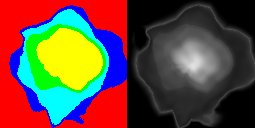
\includegraphics[width=0.6\linewidth]{terrainGAN.png}
	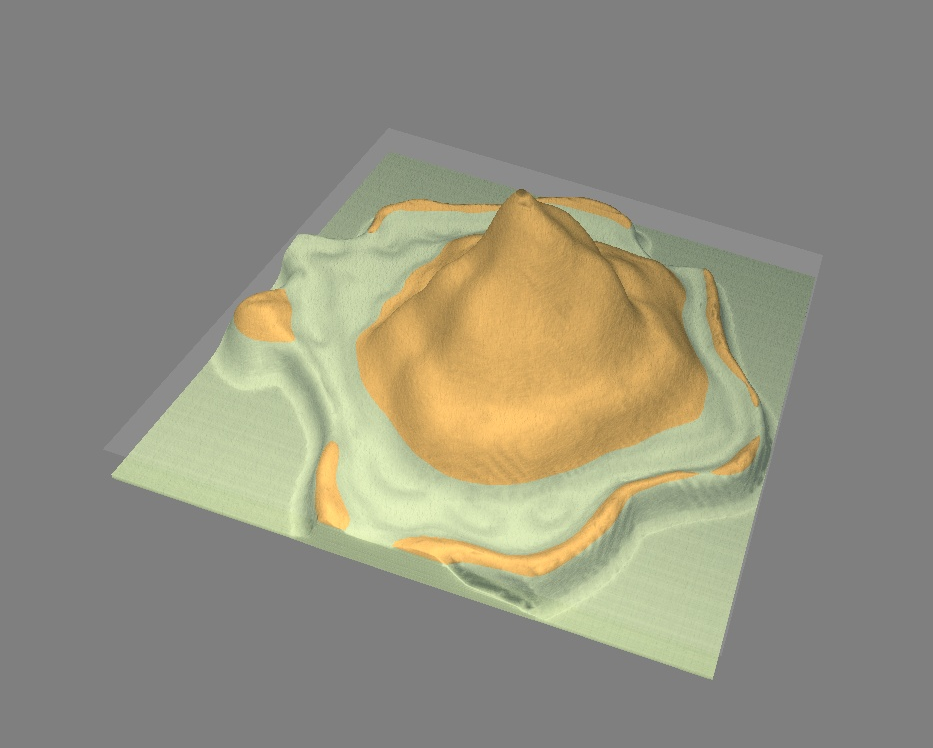
\includegraphics[width=0.3\linewidth]{terrainGAN_result.png}
	\caption{Caption.}
	\label{fig:teaser_cGAN}
}

\abstract 
In this chapter, we propose a procedural method for generating single circular volcanic islands using user sketching from two perspectives: a top view, which defines the island's shape (horizontal dimensions), and a profile view, which outlines its elevation and terrain (vertical dimensions). These perspectives, commonly used in geological and remote sensing domains, are complemented by a user-defined wind field, applied as a distortion field to deform the island's shape, mimicking the effects of wind and waves. Based on these inputs, our method generates a height field of the island. This algorithm is capable of creating many different island models, and we have generated thousands of exemplars to compose the dataset used for training a conditional Generative Adversarial Network (cGAN). By applying data augmentation, the cGAN allows for even greater variety in the generated islands, providing users with more control over the shape and structure of the final output.
\pagebreak 

\minitoc

\section{Introduction}
\label{sec:coral-island_introduction}

Coral reef islands are formed through a dynamic interplay of volcanic activity, coral growth, and long-term geological processes. These islands begin as volcanic landmasses, created when magma from the Earth's mantle erupts through the ocean floor and builds up layers of volcanic rock, eventually rising above sea level. In tropical waters, these volcanic islands create ideal conditions for coral reefs to develop. Corals, thriving in the shallow, sunlit waters around the island, initially form fringing reefs attached to the island's coastline.

As time passes, the volcanic island undergoes subsidence, a slow sinking process caused by the cooling and contraction of the Earth's crust beneath the island. In response to this subsidence, corals continue to grow upward, maintaining their position within the photic zone, where sunlight supports their survival. This upward growth leads to the formation of barrier reefs, which become separated from the island by a lagoon as the island sinks further.

Eventually, the volcanic island may submerge completely beneath the ocean's surface, leaving only the coral structure visible above water. This process results in the formation of atolls, which are ring-shaped reefs encircling a central lagoon. Over geological time, the physical structure of the island evolves from a prominent volcanic peak to a coral-dominated reef system, shaped by the combined forces of subsidence, coral growth, and erosion.

% 
Charles Darwin's subsidence theory, developed from his observations during the voyage of the HMS Beagle, remains one of the most widely accepted explanations for the formation of coral reef islands. Darwin proposed that coral reefs form around volcanic islands that slowly subside over time due to geological processes. As the volcanic island sinks, coral reefs grow upward, maintaining their position near the surface of the ocean. This theory explains the transition from fringing reefs attached to the island's coast, to barrier reefs separated by a lagoon, and finally to atolls, where the volcanic island has completely submerged, leaving only the coral structure visible above water.

While other theories, such as John Murray's growth on submerged mountains and Reginald Daly's sea level change theory, have also been proposed to explain coral reef formation, Darwin's subsidence theory remains the most widely supported due to its ability to account for the full evolution of coral islands, from volcanic landmasses to atolls. Its simplicity and focus on the relationship between subsidence and coral growth make it especially well-suited for computational modeling.

In our approach, we translate the core principles of Darwin's theory into a procedural generation model, simulating the gradual sinking of volcanic islands while coral reefs grow to keep pace with changing sea levels. This allows us to realistically model the transformation of islands from volcanic landmasses to coral-dominated atolls. By capturing this interplay, we can procedurally generate a wide variety of island structures that reflect real-world geological processes.

%

Simulating the formation of coral reef islands presents significant challenges due to the complex interplay of geological, environmental, and biological factors. One major difficulty lies in capturing the long-term subsidence of volcanic islands, which occurs over millions of years, while simultaneously modeling the upward growth of coral reefs that rely on environmental conditions such as water depth, temperature, and sunlight. This combination of slow geological processes and dynamic biological growth is difficult to replicate in a computational model.

Additionally, the biological aspects of coral growth are inherently tied to environmental factors. Coral reefs grow only within a specific range of water depth and sunlight, and their growth patterns are affected by the health of the reef ecosystem and the availability of resources. Accurately modeling these biological dependencies in a procedural system is challenging, as the factors governing coral reef development are difficult to generalize.

Existing terrain generation methods, such as Perlin noise-based algorithms or uplift-erosion models, are often ill-suited for these processes. While they can generate natural-looking landscapes, they do not account for the unique geological and biological interactions that govern coral island formation. Capturing these dynamics requires a balance between realism and procedural flexibility, allowing for both accurate simulation of natural processes and intuitive user control.

%

To address these challenges, we present a procedural generation tool that simulates the formation and evolution of coral reef islands by integrating both geological and biological processes. Our approach allows users to control the island's shape and structure through intuitive sketching interfaces, while the tool handles the complex dynamics of subsidence, coral growth, and environmental deformation.

The generation process begins with two user-defined inputs: a top view to outline the island's overall shape and a profile view to define its elevation and terrain contours. These inputs serve as the foundation for creating a height field of the island. Additionally, a wind deformation field allows the user to simulate the effects of wind and waves, reshaping the island's structure in a way that mimics natural erosion processes.

To enhance flexibility and allow for more complex, non-circular island structures, we incorporate a conditional Generative Adversarial Network (cGAN) into the generation process. The cGAN is trained on a dataset of islands generated by the initial algorithm, augmented to introduce a wider variety of shapes and features. This machine learning component allows for the automatic generation of diverse island models, removing some of the constraints of the initial procedural algorithm such as strictly radial symmetry while maintaining user control over key aspects of the design.

By combining user input with the adaptive power of the cGAN, our tool generates realistic coral islands that evolve from volcanic landmasses to coral-dominated atolls, capturing both geological and environmental processes.



\section{Overview}
Our system for generating coral reef islands combines user-driven sketching, procedural techniques, and deep learning to create realistic and varied island terrains. The process begins with the user sketching key features of the island, such as its overall shape and profile. This sketching process allows the user to define the layout of the island in an intuitive way, providing control over the placement of important elements like the island borders, beaches, lagoons, and coral reefs.

Once the user's sketch is complete, the system converts these high-level features into a labeled map, where each pixel is assigned to a specific region of the island. This map serves as the input to a conditional Generative Adversarial Network (cGAN), which is responsible for generating the fine details of the terrain. The cGAN has been trained on a dataset of island examples generated by the initial procedural algorithm, allowing it to produce realistic terrains that reflect the user's design while introducing natural variation and complexity.

By conditioning the cGAN on the user-defined map, the system maintains the overall structure and regions specified in the sketch, while generating realistic transitions between different areas (such as beaches, lagoons, and the island's interior). The use of deep learning, in combination with procedural techniques, allows the system to create coral islands that are both geologically plausible and tailored to the user's input.

This method provides a flexible yet powerful approach to island generation, enabling the creation of diverse island structures that reflect real-world geological processes, such as volcanic subsidence and coral reef growth.



\section{Related works}
Procedural generation of terrain has been a well-researched area in computer graphics and simulations, where the goal is to create large, realistic landscapes with minimal manual input. Various methods have been developed over the years to generate terrains automatically, from noise-based approaches to physically-based erosion simulations, sketch-driven methods, and more recently, deep learning techniques.

However, each of these techniques has its strengths and limitations, particularly when it comes to modeling coral reef islands. Coral islands present unique challenges due to the combination of long-term geological processes (such as subsidence and coral reef growth) and environmental interactions (like erosion caused by wind and waves). In this section, we review the key techniques that have been applied to terrain generation, highlight their limitations for coral island formation, and position our work as an approach that addresses these challenges.

\subsection{Noise functions}
% Noise functions
Noise-based procedural generation remains one of the most widely used techniques for creating natural-looking terrains. Introduced by Ken Perlin, the Perlin noise and Simplex noise are foundational algorithms that generates pseudo-random yet continuous variations across a grid, producing terrain features that resemble organic landscapes \cite{Perlin1985,Perlin2001}.

Beyond basic noise functions, more advanced techniques, such as Fractal Brownian Motion (FBM), are commonly used to add additional detail to terrains. FBM combines multiple layers, or "octaves," of noise at different frequencies, creating terrains with finer details and more realistic features. Noise functions are often paired with falloff maps to generate island-like terrains, where the height of the terrain gradually decreases toward the edges, mimicking the appearance of coastlines and providing a simple way to create basic island shapes.

Despite their widespread use, noise-based methods have significant limitations when applied to the simulation of coral reef islands. While these techniques excel at producing large, varied landscapes quickly, they lack the geological accuracy needed to model real-world processes like volcanic subsidence and coral growth. These approaches generate random patterns, but are disconnected from the actual physical processes that govern coral island formation.

Our approach goes beyond the randomness of noise-based generation by incorporating real-world geological and biological processes into terrain formation. Specifically, we model the gradual subsidence of volcanic islands and the upward growth of coral reefs, which are essential for representing the long-term evolution of coral reef islands. By integrating these processes into the generation algorithm, we create terrains that are not only more realistic but also allow for user control. This blend of user input and geological grounding provides a more accurate and flexible approach to modeling coral reef islands, addressing the limitations inherent in traditional noise-based techniques.

\subsection{Erosion simulation}
% Erosion simulation
While noise functions generate random, natural-looking terrain, they often fail to capture the physical processes that shape real landscapes over time. To address this limitation, erosion simulations model how natural forces such as water flow and gravity wear down terrain features, creating valleys, river networks, and other detailed landforms. These simulations are particularly effective at representing mountainous landscapes, where erosion gradually sculpts the terrain over long periods of time, typically on the scale of thousands to millions of years.

Erosion simulations often use models like the Stream Power Law to describe how water erodes higher elevations and deposits sediment in lower areas. The rate of erosion depends on factors such as slope steepness and water flow, with steeper slopes and greater water volumes leading to faster erosion. Over time, these processes create detailed and realistic terrain features like river valleys and erosion channels. Erosion models are iterative, simulating the gradual shaping of landscapes by continuously balancing forces like erosion and uplift, as seen in the work of \cite{Cordonnier2016,Cordonnier2017a}. Their model simulates how tectonic forces uplift terrain, which is then eroded away over thousands of years. Similarly, \cite{Schott2023} and \cite{Tzathas2024} refined the Stream Power Law to generate realistic slopes and ridges through these long-term geological processes.

Despite their effectiveness in modeling large-scale terrain evolution, erosion simulations are limited when it comes to representing environments that are shaped by dynamic biological processes. Coral reefs, for instance, grow and adapt to changing environmental conditions on a much shorter timescale than geological erosion. While erosion models simulate terrain changes over millennia, coral growth responds more dynamically to factors like water depth, light availability, and temperature on scales ranging from years to decades. These biological factors are difficult to incorporate into traditional erosion models, which are designed to simulate the slow, steady forces of water and gravity.

Our approach builds on the concept of terrain evolution by integrating the geological and biological dynamics that shape coral reef islands. Instead of focusing solely on erosion, which is primarily a surface-level process, we model the subsidence of volcanic islands over geological time and the simultaneous growth of coral reefs that adapt to the changing sea levels. Coral reefs must grow upward to remain within the photic zone, a process that unfolds on shorter timescales than those captured by standard erosion simulations. Furthermore, we introduce wind deformation to simulate the effects of environmental forces like wind and waves, which dynamically reshape the island's structure over time. This combination of long-term geological processes and short-term biological responses provides a more comprehensive simulation of coral reef island formation, capturing both the slow subsidence of volcanic landmasses and the rapid adaptability of coral ecosystems.

\subsection{Sketching}
% Sketching

In procedural terrain generation, sketch-based approaches allow users to directly interact with and shape landscapes through intuitive sketching interfaces. These methods enable users to define key terrain features such as mountains, valleys, and coastlines by drawing them in a two-dimensional canvas, which are then translated into 2.5D terrains. Sketching provides a high level of artistic control, making it especially popular in creative applications such as video games and simulations, where user-defined terrain features are prioritized.

Sketch-based systems offer great flexibility, allowing users to directly define specific elements of the landscape according to their needs or preferences. For instance, \citep{Gain2009} introduced a multi-perspective sketching system that allows users to generate detailed landscapes by sketching from different angles. This method provides more control over the terrain's shape than traditional noise-based generation methods. Similarly, \citep{Tasse2014} explored sketching from the player's viewpoint, allowing users to dynamically define height information from within the virtual environment, creating an interactive terrain design experience.

Sketching has also been extended to geological modeling. \citep{Patel2021} proposed a system where users can interactively model underground layers by sketching subsurface structures. This provides a powerful tool for geologists and designers who need to model complex, multi-layered terrains, offering more control over both the surface and the subsurface.

In our work, we leverage the flexibility of sketching to define the key features of coral reef islands, such as the island shape, lagoons, and coral reefs, in a vectorized format. This is particularly important for modeling underwater and island landscapes, where these features are not simply surface elements but part of an evolving geological structure. By using sketches, we retain the semantic information of where the island and coral regions are located, which allows us to later apply our simplified model of Darwin's subsidence theory.

Rather than focusing on detailed long-term or short-term evolution, our method adapts sketching to the unique requirements of island and underwater landscapes. Once the user defines the terrain layout through sketching, we apply a simplified subsidence model, where the volcanic island gradually sinks and coral reefs grow in response, remaining close to the water surface. This process provides a framework for simulating the evolution of the landscape in a geologically plausible manner.

The key advantage of sketching in our system is that it combines the artistic control provided by traditional sketching methods with the ability to handle the geological processes specific to coral reef islands. By preserving the vectorized information from the sketch, we can accurately place and evolve features like lagoons and coral reefs, ensuring that the resulting terrain reflects both the user's design intent and the geological dynamics at play.

\subsection{Deep learning}
% cGAN

In recent years, deep learning has become a transformative tool in computer graphics, image processing, and procedural content generation. Deep learning refers to a class of machine learning techniques that use artificial neural networks with multiple layers to model complex patterns in data. By training these networks on large datasets, deep learning models can learn to generate new, realistic data by identifying the underlying relationships between inputs and outputs.

In terrain generation, deep learning is particularly well-suited to tasks that require the creation of complex, natural-looking landscapes. Traditional procedural generation techniques like noise functions and erosion simulations can be powerful, but they often struggle to produce the complexity and realism of natural terrains due to their reliance on predefined rules and algorithms. In contrast, deep learning models, especially Generative Adversarial Networks (GANs), can learn from data, enabling them to generate realistic terrains that mimic the diversity and complexity found in nature.

GANs are a particularly effective deep learning architecture for terrain generation. A GAN consists of two neural networks: a generator, which creates new data samples, and a discriminator, which evaluates whether the generated samples are real or fake compared to a set of training data. Through this adversarial process, the generator gradually improves its ability to produce realistic examples, while the discriminator becomes better at distinguishing real from fake data. This feedback loop allows GANs to generate highly realistic and detailed terrain features by learning from large datasets of existing terrains.

In terrain generation, GANs have been applied to generate diverse landscapes by learning the patterns and features found in real-world terrains. For example, \citep{Guerin2017} demonstrated how GANs can be used to transform 2D sketches into 3D terrains by training the network on a dataset of terrain features, allowing the system to generate new landscapes based on simple user input. GANs are particularly well-suited for this task because they can capture the subtle details of terrain that would be difficult to model explicitly, such as the natural flow of elevation or the transitions between different terrain types.

A variant of GANs, known as Conditional Generative Adversarial Networks (cGANs), takes the power of GANs one step further by allowing the generated data to be conditioned on additional inputs. In a cGAN, both the generator and the discriminator receive additional information such as a class label, a sketch, or an image, that guides the generation process. This makes cGANs particularly useful for terrain generation tasks where users want to control specific aspects of the output while still relying on the model to generate realistic details.

In the case of terrain generation, a cGAN allows the user to specify high-level constraints (such as the outline of an island or the regions where different terrain types should be) while the generator fills in the finer details based on what it has learned from the training data. This makes cGANs particularly effective in applications where a mix of user input and data-driven generation is required, as the user can control the broad layout of the terrain while the model ensures that the resulting terrain looks natural and plausible.

In our approach, we use a cGAN to generate coral reef islands, providing a balance between user control and realistic terrain generation. After the initial algorithm outlines the regions of the island such as the island itself, beaches, and lagoons, these regions are transformed into a single image, where each pixel represents a different region ID. This image is used as the input for the cGAN, which conditions the generation process on this initial layout.

The cGAN is trained on a dataset of island examples, which are created by the initial procedural generation algorithm and further augmented to introduce a wide variety of shapes and features. This training allows the cGAN to generate coral reef islands that follow the high-level layout provided by the user while introducing natural variations and details that reflect real-world island characteristics. By conditioning the cGAN on the user-defined region map, we ensure that the generated islands maintain structural coherence while still exhibiting realistic features like smooth transitions between regions, varied terrain, and non-circular shapes.

One of the key advantages of using a cGAN in our system is its ability to overcome procedural constraints. Traditional procedural generation methods often impose limitations like radial symmetry or require islands to follow overly simplified geometries. With the cGAN, these constraints are lifted. The model can generate irregular, non-circular islands that adhere to the user's input but introduce a level of complexity and realism that would be difficult to achieve with purely procedural methods.

Additionally, the cGAN ensures that the generated island terrain aligns with the geological processes modeled in the system, such as subsidence and coral reef growth. By training the cGAN on thousands of examples that reflect these processes, we ensure that the final generated island models are both flexible and geologically plausible. The combination of user-driven design and data-driven generation through the cGAN allows for the creation of coral reef islands that are not only tailored to the user's input but also realistic in their form and structure.



\section{Example generation}
\label{sec:coral-island_example-generation}

Generating synthetic coral reef island terrains involves a combination of user input, procedural techniques, and simplified geological simulations. The process begins with the creation of a base terrain using user-defined sketches, followed by a simulation of coral reef growth and subsidence. These two steps, although interconnected, can also be used independently, providing flexibility in how the system is applied. In this section, we describe the example generation process in detail.

\subsection{Assumptions}
In generating synthetic coral reef islands, we adopt a set of simplifying assumptions that are grounded in geological and biological observations. These assumptions streamline the process while producing plausible terrains. Below, we outline the key characteristics of our model:

% \begin{itemize}
    \textit{Radial symmetry:} Volcanic islands often begin as circular landmasses due to the radial uplift of magma from beneath the Earth's mantle. Erosion processes further smooth out sharp edges over time, reinforcing this initial symmetry. In our approach, we assume islands start with an approximately circular shape, providing a straightforward basis for terrain generation.
% This assumption reflects real-world volcanic islands, such as those in the Pacific, where erosion gradually shapes the initial circular form. Starting with a radial structure simplifies the generation and serves as a solid foundation for further deformation.

    \textit{Coral growth at constant depth:} Coral reefs require sunlight to thrive, which limits their growth to depths where light penetrates the water. In our model, coral growth is constrained to this depth range, with corals maintaining their proximity to the water surface as the volcanic island subsides.
% Coral growth follows biological principles, growing upward in shallow waters. This assumption simplifies the process of modeling coral features and reflects the observed behavior of real coral reefs.

    \textit{Radial arrangement of features:} The key island features like the island body, beaches, lagoons, and coral reefs, are arranged in concentric regions around the island center. This radial arrangement aligns with natural geological progression from the island to the surrounding reef.
% This simplifies the generation process by organizing features in a predictable order, similar to coral atolls where lagoons and reefs form protective rings around the island.

    \textit{Wind and wave deformation:} Over time, wind and wave forces shape islands by introducing concave regions, carving out lagoons, and deforming coastlines. To simulate these effects, we apply a wind deformation field that allows users to introduce natural variations that break the radial symmetry, resulting in more realistic island shapes.
% Wind and wave erosion play a significant role in shaping real coral islands, and simulating this erosion adds natural-looking variation. The wind field gives the user control over how much deformation is applied, creating non-uniform, dynamic island coastlines.

    \textit{Independence of islands:} In this model, each island is treated as an independent entity, meaning its terrain does not influence neighboring islands. This allows multiple islands to be generated and placed freely without concern for terrain overlap or interaction. 
% This assumption reflects the typical formation of islands in archipelagos, where individual islands are geographically separate. It simplifies the generation of multi-island scenes by avoiding unnecessary inter-island interactions.

    \textit{Uniform profile shape:} We assume that the vertical profile of the island remains relatively uniform, meaning that the terrain's cross-section from the center outward is similar in every direction. This allows for consistent scaling of the profile in all directions, ensuring that the island's shape remains coherent and plausible.
% Although real-world islands can have local variations in their profile, this uniformity makes the generation process more manageable and produces consistent terrain features.

    \textit{Subsidence and coral growth:} As the volcanic island subsides, coral reefs grow to keep pace with the sinking landmass, maintaining their height near the water surface. In our model, the island subsides as a whole, while coral features are preserved by growing vertically. This separation allows the coral regions to remain unaffected by the subsidence of the island itself.
% This assumption is based on Darwin's subsidence theory, which explains the formation of coral atolls. Modeling coral growth independently of the island's subsidence ensures the coral regions stay at the water surface as the island sinks.
% \end{itemize}

These assumptions, while simplified, provide an effective foundation for generating coral reef islands. They balance computational efficiency with geological plausibility, ensuring that the generated terrains are both flexible and realistic. Furthermore, the system allows users to break the radial symmetry and introduce more natural variations through wind deformation, adding another layer of flexibility to the model.


\subsection{User Input}

The generation of coral reef islands in this system begins with two intuitive sketch-based inputs from the user: a top-view sketch and a profile-view sketch, which define the islands horizontal layout and vertical elevation profile. In addition to these sketches, the user can further refine the terrain by applying wind deformation strokes, which simulate the effects of wind and waves on the islands shape. This combination of sketches and wind inputs gives users precise control over both the islands structure and its natural variations, such as irregular coastlines or concave features.

\subsubsection{Top-view Sketch}

The top-view sketch defines the islands outline as seen from above. Using a simple drawing interface, the user can delineate the boundaries between key regions of the island, including the island itself, the beaches, the lagoon, and the surrounding abyss. The system assumes that these regions are arranged concentrically around the center of the island, with each boundary defined by a radial distance from the center.

Each region's boundary is represented in polar coordinates, with $\radius_\p$ indicating the radial distance from the islands center and $\theta_\p$ representing the angular position. This polar representation allows the system to map the users sketch onto a circular framework, ensuring smooth transitions between regions and maintaining a coherent layout for the island.

In this sketch, the user defines the overall horizontal layout of the island, including the size and shape of each feature. Variations in the outline can be introduced by allowing the radial distances to vary with angle, ensuring that the island is not strictly symmetrical and introducing more natural, irregular shapes.

\subsubsection{Profile-view sketch}

The profile-view sketch defines the vertical elevation profile of the island along any radial direction, offering control over the islands height. In this view, the user specifies the elevation of different regions of the island, such as the island peak, beach, lagoon, and abyss, by marking a set of milestones along the profile.

These milestones correspond to key terrain transitions: the highest point of the island (center), the island border, the beach, the lagoon, and the deep-sea abyss. The system uses these milestones to interpolate a continuous 1D height function $\heightProfile(x)$, where $x \in [0,1]$ represents the normalized radial distance from the islands center, and $h = \heightProfile(x)$ gives the height at each point. This continuous profile ensures smooth elevation transitions across the island.

By combining the top-view and profile-view sketches, the system can generate a full 3D terrain model that accurately reflects the users design.

\subsubsection{Wind velocity field}
In addition to the sketches, the user can influence the shape of the island by defining a wind velocity field. This field simulates the effects of wind and wave erosion on the island's surface, introducing natural deformations such as coastline indentations, concave features, or variable lagoon shapes.

The wind field is represented as a series of wind strokes drawn by the user on a 2D canvas. Each stroke represents a parametric curve, where the direction and strength of the wind are encoded as a vector field. The user controls the wind's direction by drawing these curves, and the system interprets the strokes to create a velocity field that defines how the terrain should be deformed.

As the user draws a wind stroke, the system generates a set of control points along the curve, with the option to adjust the stroke's width. The width of each stroke determines the area of influence around the curve, where wider strokes result in broader deformations of the terrain.
The deformation strength decreases with distance from the wind curve using a Gaussian falloff function using the stroke width as standard deviation, ensuring that the terrain transitions smoothly from deformed regions to non-deformed areas.
Once the wind strokes are applied, the system processes the wind velocity field by displacing the terrain points accordingly. The height field, originally generated from the user's sketches, is modified by the wind field to create non-radial features, breaking the initial radial symmetry and producing a more organic island shape.

\subsubsection{User interaction}

As users draw the top-view and profile-view sketches, the system provides real-time feedback on the resulting terrain. The top-view sketch influences the horizontal layout of the island, while the profile-view sketch defines its vertical structure. These sketches can be adjusted independently, allowing the user to fine-tune both the outline and elevation of the island.

After sketching the basic shape, users can apply wind deformation strokes to modify the island's features further. These strokes represent wind and wave influences, distorting the island's shape to introduce more natural, non-radial features such as indentations along the coastline, variable lagoon shapes, or concave formations. The system automatically applies these deformations, providing real-time feedback as the user interacts with the terrain.

This interactive process, combining sketches and wind deformation, allows users to quickly iterate on their designs, refining the terrain to meet specific aesthetic or functional goals.




\subsection{Generation process}
The generation of coral reef island terrains involves a structured process that takes the user's sketches and produces a complete 3D terrain model. This process begins with the creation of the initial height field based on the user's input, followed by the application of wind deformation to introduce natural variations, and concludes with the integration of coral reef features through subsidence and coral growth modeling.

\subsubsection{Initial height field generation}
The generation of the coral reef island terrain begins by transforming the user-defined top-view and profile-view sketches into a coherent 3D height field. This process combines the radial layout of the top-view sketch with the elevation information provided by the profile-view sketch, creating a terrain that accurately represents the desired features, such as the island, beaches, lagoons, and abyss.

For any point $\p$ on the terrain, the system first computes the polar coordinates $(\radius_\p, \theta_p)$, where $\radius_\p$ is the radial distance from the island's center, and $\theta_p$ is the angular component. The radial distance $\radius_\p$ is used to determine which region the point belongs to (island border, beach, lagoon, or abyss). The user-defined milestones in the profile sketch specify the radial boundaries between these regions.

Each point's height is determined by the profile function $\heightProfile(x)$, where $x$ represents the normalized radial distance from the island's center. The function $\heightProfile(x)$ is continuous and defines the height of the terrain at any point along the profile, from the island's center (at $x = 0$) to the outer boundary of the abyss (at $x = 1$).

The system first identifies which region the point $\p$ falls into by comparing $\radius_\p$ with the radial boundaries defined by the milestones. These milestones divide the terrain into sections, such as:
\begin{itemize}
    \item Island: $\radius_\p \leq \radius_{\text{island}}$,
    \item Beach: $\radius_{\text{island}} < \radius_\p \leq \radius_{\text{beach}}$,
    \item Lagoon: $\radius_{\text{beach}} < \radius_\p \leq \radius_{\text{lagoon}}$,
    \item Abyss: $\radius_{\text{lagoon}} < \radius_\p \leq \radius_{\text{max}}$
\end{itemize}

For any point between two milestones (e.g., between the island border and the beach), the system computes the normalized distance $x_\p$ using linear interpolation between the radial distances of the two milestones. For example, if $\radius_\p$ is between the beach boundary $\radius_{\text{beach}}$ and the lagoon boundary $\radius_{\text{lagoon}}$, the value of $x_\p$ is computed as:

\begin{align}
    x_\p = \frac{\radius_\p - \radius_{\text{beach}}}{\radius_{\text{lagoon}} - \radius_{\text{beach}}}
\end{align}

This normalized distance $x_\p$ represents the position of point $\p$ relative to the region's boundaries.

Once the correct value of $x_\p$ is determined, the height of the point $h(\p)$ is computed directly using the profile function $\heightProfile(x)$, which smoothly defines the height for any given value of $x$. The height function $\heightProfile(x)$ is continuous across all regions, ensuring that transitions between the island, beach, lagoon, and abyss are smooth.

For any point $\p$, the height is computed as:
\begin{align}
    h(\p) = \heightProfile(x_\p)
\end{align}

This approach ensures that the height field accurately follows the elevation profile specified by the user while maintaining smooth transitions between different regions of the island.

By using the profile function $\heightProfile(x)$ to directly compute the height for any point on the terrain, the system guarantees smooth transitions between regions (e.g., from the island to the beach or from the lagoon to the abyss). This method eliminates the need for separate interpolation between regions, as the function $\heightProfile(x)$ is defined continuously across all regions of the island.

The result is a height field that captures both the radial structure of the island (from the top-view sketch) and the vertical elevation profile (from the profile-view sketch), producing a realistic representation of coral reef islands with smooth transitions between the key terrain features.



\subsection{Wind deformation}

After generating the initial height field based on the top-view and profile-view sketches, the next step in the process introduces wind deformation. This step simulates the long-term effects of wind and wave erosion, breaking the radial symmetry of the terrain and adding natural variations such as concave coastlines and irregular island shapes.

% \subsubsection{User-defined wind field}

The wind deformation can be controlled through a user-defined vector field, which represents the direction and strength of wind flows across the terrain. Users interact with the system by drawing strokes on a 2D canvas, which are then interpreted as parametric curves $\curve$ representing wind patterns. Each stroke defines a wind flow in the curve's direction $\curve'$ and an effect width $\std$, and these wind flows are used to displace the terrain, simulating the gradual reshaping of the island due to wind and wave erosion.

The strokes are represented as Catmull-Rom splines, a type of parametric curve that allows for smooth, continuous wind paths. For any point $\p$ on the terrain, the deformation vector $\warp(\p)$ is calculated based on the proximity of $\p$ to the nearest wind strokes. The strength of the displacement is controlled by a Gaussian scaling function, which ensures that points closer to the wind strokes experience stronger displacement, while points farther away are less affected.

The displacement $\warp(\p)$ is computed as a sum of the influences from all nearby wind strokes. For each stroke, the deformation vector is scaled by a Gaussian function that decreases with the distance from the closest point $\q$ on the parametric curve $\curve$, as follows:

\begin{align}
    \warp(\p) = \sum_{\curve \in \text{curves}} \curve'(\q) \cdot e^{-\frac{\norm{\p - \q}^2}{2 \std^2}}
\end{align}


% \subsubsection{Deformation process}
Once the deformation vector $\warp(\p)$ is computed, the terrain height at point $\p$ is adjusted by displacing $\p$ to a new point $\warp(\p)$.
We can then compute the final height $h(\warp \circ \p) = \heightProfile(t_{\p})$, or, as the implicit modeling community would write it, 
\begin{align}
    \Tilde{h}(\p) = \warp^{-1} \circ h
\end{align}

This process introduces variations in the terrain, distorting the coastline, creating concave regions, and breaking the original radial symmetry defined by the top-view and profile-view sketches.

\subsubsection{Resistance to deformation}

To ensure that certain regions of the terrain, such as deep-water areas, remain relatively unaffected by the wind, a resistance function $\rho(x)$ is applied. The resistance function modulates the effect of the wind deformation based on the radial distance $\radius_\p$ from the island's center, which is normalized to a value $x \in [0, 1]$.

The resistance function $\rho(x)$ is defined similarly to the profile function, and it controls the magnitude of the displacement at each point. For example, regions near the coastline (such as the beach and lagoon) might have lower resistance, allowing for more significant deformation, while regions farther away (such as the abyss) have higher resistance, limiting the wind's impact.

The deformation vector is scaled by the resistance function at each point $\p$, such that the final deformation vector becomes:

\begin{align}
    \Tilde{\warp}(\p) = \rho(x_\p) \cdot \warp(\p)
\end{align}

Where $\rho(x_\p)$ is the resistance value corresponding to the point's normalized distance $x_\p$. This ensures that the wind deformation has the greatest impact on areas like the coastline and beach, where erosion naturally plays a larger role, while deeper regions like the abyss remain stable and relatively unchanged.

\subsubsection{Deformation and height field update}

The wind deformation process results in a modified height field where the terrain has been warped according to the user-defined wind strokes. This deformation introduces non-radial features, such as concave coastlines or irregularities along the beach and lagoon, making the island appear more natural and varied.

Both the height field and the labeled map (which tracks the terrain regions like island, beach, and lagoon) are updated to reflect the wind deformation. This ensures that the semantic information of the terrain remains consistent even after the terrain has been warped. The labeled map is deformed in the same way as the height field, preserving the logical structure of the island for further post-processing, such as texturing.

For instance, consider a simple circular island generated from the initial height field. By applying wind strokes along one side of the island, the deformation process can create concave regions along the coastline, making the shape more irregular and mimicking the effects of real-world wind and wave erosion. The resistance function ensures that while the beach and lagoon areas are deformed, the abyss remains largely unaffected as they are far from the wind and wave effective areas, preserving the island's overall structure.




\subsection{Coral reef modeling}

Once the terrain has been generated and deformed by the wind, the system simulates the subsidence of the volcanic island and the growth of coral reefs. These processes reflect the long-term geological evolution of coral reef islands, where the volcanic island gradually sinks (subsides) while coral reefs grow upward to keep pace with the sinking landmass.

\subsubsection{Subsidence}

The subsidence of the island is modeled by scaling the initial height field downward, simulating the effect of the volcanic island slowly sinking into the ocean. The user provides a subsidence rate $\lambda$, which represents the proportion by which the island has sunk over time. The subsidence is applied uniformly to the terrain, meaning all points on the island sink by the same factor.

The subsided height field $h_{\text{subsided}}(\p)$ is computed by scaling the original height field $h_0(\p)$ with the subsidence factor $\lambda$:

\begin{align}
h_{\text{subsided}}(\p) = (1 - \lambda) \cdot h_0(\p)
\end{align}

Where:
- $\lambda \in [0, 1]$ is the subsidence rate (e.g., $\lambda = 0.2$ means the island has subsided by 20% of its original height),
- $h_0(\p)$ is the height at point $\p$ from the initial height field.

This scaling reduces the overall height of the island, simulating how volcanic islands sink over time due to tectonic activity and erosion. The subsidence factor $\lambda$ is applied uniformly across the terrain, meaning that all points on the island experience the same degree of subsidence, regardless of their original height or location.

\subsubsection{Coral reef growth}

As the volcanic island subsides, coral reefs grow upward to remain close to the water surface, following the “keep-up” strategy observed in real-world coral formations. Coral growth is restricted to regions where the depth is within the optimal range for coral development, typically from the water surface to around 30 meters below.

The coral reef features (reef crest, back reef, and fore reef) are modeled separately from the subsidence process. The system generates a coral feature height field $h_{\text{coral}}(\p)$, which remains unaffected by the island's subsidence. This height field ensures that coral regions remain near the water surface, even as the island sinks.

Coral reef growth is entirely independent of the subsided terrain. Even as the volcanic island sinks, coral growth is driven only by the proximity of terrain to the water surface, ensuring that coral features always remain near the surface, irrespective of how much the island subsides.

The coral reef height field is generated using predefined depth values for the various coral regions:
- The reef crest is modeled near the water surface, typically just below sea level,
- The back reef and lagoon are slightly deeper but remain within the range where corals can grow,
- The fore reef slopes downward into the deep ocean, transitioning into the abyss.

The system uses these predefined regions to assign heights to coral reef points based on their proximity to the reef crest. For example, the height of a point in the fore reef is interpolated between the reef crest height and the deeper abyss regions.

\subsubsection{Blending the height fields}

The final step is to blend the subsided height field $h_{\text{subsided}}(\p)$ with the coral feature height field $h_{\text{coral}}(\p)$ to produce the final terrain. The goal is to ensure that coral features remain near the water surface while allowing the rest of the island to subside.

To achieve this, the system uses a smooth max function, which smoothly blends the two height fields. The smooth max function ensures that the coral regions dominate where coral growth is present, while the subsided island terrain dominates in other regions. This blending method ensures that the transition between the coral and subsided regions is smooth and visually consistent.

The smooth max function adapted from Ingo Quilez's smooth min function is defined as:

\begin{align}
    \smoothmax(a, b, k) = a + \frac{(b - a)}{1 + \exp\left(-k \cdot (b - a)\right)}
\end{align}

Here, $a = \heightSubsid(\p)$ is the height from the subsided island, $b = \heightCoral(\p)$ is the height from the coral reef feature, and $k$ controls the smoothness of the transition.

This smooth max function guarantees visual continuity by preventing abrupt height differences between the coral regions and the subsided terrain, creating a smooth, gradual transition that mimics the natural blending of coral reefs with deeper areas. The coral feature height field takes precedence where coral can grow, typically in shallow regions up to around 30 meters below the water surface. In deeper regions, such as the abyss, the subsided height field naturally dominates, ensuring that the final terrain accurately reflects both subsidence and coral growth processes.

\subsubsection{Output}

The resulting terrain represents a realistic coral reef island, where the volcanic island has subsided, and coral reefs have grown upward to keep pace with the water level. The smooth blending between the subsided terrain and the coral features ensures a natural transition between regions like the island, lagoon, and coral reefs.

One of the key strengths of this method is its flexibility: 
- The subsidence and coral reef growth processes are modeled independently, allowing for a wide range of configurations. Users can generate plausible island terrains with or without coral features, or apply the coral reef growth simulation to existing height fields from other sources.
- Additionally, the coral reef growth simulation can be fine-tuned by adjusting the predefined depth values for different coral regions, allowing for further customization of the terrain's appearance.





\section{Conditional Generative Adversarial Networks}

In this section, we introduce the use of a Conditional Generative Adversarial Network (cGAN), specifically the pix2pix model, to enhance the island generation process by increasing the variety and flexibility of terrains. While the initial procedural algorithm can create numerous island examples, cGAN provides additional flexibility in generating more complex terrain without the rigid constraints of the first algorithm.

\subsection{Introduction to cGAN}

A Generative Adversarial Network (GAN) consists of two competing neural networks: a generator that attempts to produce realistic data, and a discriminator that tries to distinguish between real and generated data. In the conditional GAN (cGAN) variant, both the generator and discriminator are conditioned on some input, meaning the generated output is influenced by additional information, such as a labeled map or image.

For island generation, we use the pix2pix model, a specific cGAN designed for image-to-image translation. In this case, the input to the generator is a labeled map which is a 2D image where each pixel is assigned an ID representing a different region of the island (e.g., island body, beach, lagoon, coral reef). The output is an image where each pixel corresponds to the elevation of the terrain at that point, ie. a height field.

\subsection{cGAN for island generation}

The cGAN model was chosen for this task because it allows us to overcome some of the constraints of the initial procedural algorithm. While the first algorithm generates island terrains based on radial symmetry and a limited set of input parameters, cGAN can generate more complex and varied terrains by learning from a large dataset of examples. Specifically, the use of cGAN addresses the following challenges:

1. Increased Variety: The cGAN model can generate a wide range of island shapes and terrains by learning from the dataset. This allows for the creation of terrains that go beyond the predefined structures of the initial algorithm, introducing more natural variation in island features.

2. Overcoming Constraints: In the initial algorithm, islands are always centered in the image and adhere to a radial symmetry. Using cGAN, we apply data augmentation (translation, scaling, and combining multiple islands in one sample) to remove these constraints, allowing islands to take more irregular shapes and positions.

3. Flexibility: Once trained, the cGAN model acts as a black box that generates island terrains based on the labeled input. While this limits user control during the generation process, the model can produce a variety of terrains that still respect the underlying structure of the labeled map. This enables a flexible, rapid generation process without requiring the user to fine-tune parameters manually.

\subsection{Training}

The cGAN model is trained using a dataset of island terrains generated by the initial algorithm. To create this dataset, the algorithm randomly generates top-view shapes for the island's features, adds noise (such as fractional Brownian motion, or fBm), and introduces random wind velocity fields. The profile function remains consistent in determining the relative positions of the island, beach, and lagoon, but the top-view shapes vary through noise and deformation.

\subsubsection{Data augmentation}

To enhance the variety of the dataset and improve the model's ability to generalize, we apply several data augmentation techniques:
- Translation: Since the original algorithm always centers the island, we translate the islands within the image to remove this constraint. This ensures that the cGAN can generate islands in any position within the frame.
- Directional Scaling: By scaling the terrain in one direction, we create elongated islands that resemble corridors or archipelagos, adding another layer of diversity to the dataset.
- Multiple Islands per Sample: In some cases, we combine multiple islands into a single sample, ensuring they do not overlap. The regions not covered by any island are assigned the abyss ID. Although this approach ensures non-overlapping regions, future work could explore using blending techniques to position islands more closely without the risk of overlap.

All augmentation techniques are applied both to the height field and the labeled map simultaneously to ensure consistency between the input (labeled map) and the output (height field).

\subsection{Model output}

Once trained, the cGAN model generates a height field from a given labeled map. The output is a complete 2D height map representing the terrain's elevation at each point. Although the cGAN works as a black box, the labeled map remains available after inference and retains valuable information for the user.

The labeled map can be used for post-processing tasks, such as:
\begin{itemize}
    \item Texturing: Different regions of the terrain (e.g., beach, lagoon, coral reef) can be textured based on their region ID from the labeled map, allowing for detailed terrain decoration.
    \item Material Information: The labeled map can provide cues about the underlying ground material in each region, which can be useful for additional simulations, such as erosion or weathering.
\end{itemize}

However, it's important to note that the current implementation of the cGAN does not allow for user control during the generation process itself. The model takes the labeled map as input and outputs a height field without any additional parameters that the user can adjust in real-time. While this limits user interaction, the resulting terrains are still varied and flexible thanks to the data diversity learned during training.

\subsection{Limitations}

While the cGAN model provides increased flexibility and variety in island generation, it does come with certain limitations:

\begin{itemize}
    \item Biases from the synthetic dataset: Since the cGAN model is trained entirely on a procedurally generated dataset, it inherits the biases present in the initial algorithm. For example, while the model can break free from the radial symmetry constraint and center positioning, it still relies on the synthetic data's structure and patterns. This can limit the true diversity of the generated terrains, as the cGAN cannot generate terrains that deviate too far from the examples in the training set.
    \item Lack of user control: Another limitation of using cGAN in this context is the lack of real-time user control during terrain generation. While traditional procedural generation methods allow users to tweak parameters (e.g., island size, beach width) during the generation process, the cGAN model operates as a black box, providing no mechanism for direct user interaction beyond the initial labeled map. This reduces the level of customization available to the user.
    \item Data-driven dependence: The quality of the generated terrain depends entirely on the quality and variety of the training dataset. Since the dataset is synthetically generated, any limitations or biases in the initial dataset directly affect the cGAN's output. This dependence on data quality makes it crucial to design a well-augmented and varied dataset to ensure diverse and realistic outputs.
\end{itemize}



\section{Conclusion}

This work has presented a novel approach to generating coral reef island terrains by combining traditional procedural methods with deep learning techniques. We first developed a procedural generation algorithm capable of creating a wide variety of island terrains through a combination of top-view and profile-view sketches, wind deformation, and subsidence and coral reef growth simulation. By applying these methods, we were able to produce realistic terrains based on geological processes, capturing key features of coral reef islands such as beaches, lagoons, and coral reefs.

To further enhance flexibility and realism in the generation process, we incorporated a Conditional Generative Adversarial Network (cGAN), using the pix2pix model to generate height maps from labeled maps of island features. The cGAN model allowed us to overcome some of the constraints inherent in the procedural algorithm, such as radial symmetry and fixed island positioning. With data augmentation techniques, we were able to train the cGAN on a synthetic dataset, generating varied and realistic island terrains.

\subsection{Advantages of the approach}

One of the main strengths of this approach is its ability to produce a wide variety of island terrains, even in the absence of real-world data. The procedural generation methods allow for high flexibility in designing both the shape and features of the island, while the use of cGAN enables further refinement and the generation of terrains that are not bound by the original constraints of the procedural model. By combining these two methods, we leverage the advantages of both: the structured control of procedural techniques and the pattern-learning capabilities of deep learning.

A key advantage of this approach is the retention of semantic information about the terrain throughout the generation process. The labeled map, which serves as the input to the cGAN, can also be used after terrain generation to provide a detailed representation of the different regions of the island (such as the beach, lagoon, coral reef, and island body). This labeled map can guide post-processing operations, such as applying different textures based on terrain features or adding other environmental elements like vegetation. The preservation of semantic information provides a useful connection to the next stage of terrain manipulation, making the process more versatile and adaptable to different use cases.

Furthermore, the use of an out-of-the-box cGAN model highlights the feasibility of employing existing neural network architectures with minimal modifications in the field of procedural generation. This is particularly important in domains where real-world data is scarce, such as coral reef islands, allowing synthetic data to be effectively used for training purposes.

\subsection{Limitations}

While this approach brings significant advantages, there are also some limitations to consider. The reliance on a synthetic dataset means that the cGAN inherits the biases and limitations of the original procedural algorithm. This could limit the true diversity of the terrains that the model can generate, as the output is confined by the patterns present in the training data. Additionally, the cGAN model functions as a black box, offering limited user control over the generation process once the model has been trained. This contrasts with traditional procedural methods, which typically allow for real-time tweaking of parameters.

\subsection{Future works}

There are several directions for future research and improvements. One promising avenue is to incorporate the wind velocity field more directly into the cGAN training process, potentially as an additional input condition. This would allow the model to better capture wind-driven terrain features such as cliffs or other deformations influenced by wind patterns.

Another area for exploration is improving user interaction during the terrain generation process. While the current model allows for rapid terrain generation, adding more options for users to interact with the cGAN, such as tweaking parameters like wind strength or island size, could enhance the flexibility of the system.

Finally, further improvements could be made to the synthetic dataset. Incorporating more complex geological processes, such as wave erosion or tidal influences, could lead to even more realistic terrains. Additionally, refining the way islands are blended in multi-island samples, or adding more diverse input conditions (e.g., different geological settings), could help the model generalize better and produce more varied and dynamic landscapes.


One possible future improvement could involve incorporating the wind velocity field into the cGAN training process. While the labeled map is the only input used in the current implementation, the wind field could be added as an additional condition. This would be especially useful if the initial algorithm were augmented to include wind-driven features, such as cliffs or specific terrain deformations influenced by wind patterns. Adding the wind field as an input could help the cGAN generate more realistic terrains that better reflect the influence of wind on the landscape.

Additionally, further development could explore improving how multiple islands are combined in a single sample. For example, using blending techniques to handle overlapping regions could allow islands to be positioned closer together, enabling the generation of more complex archipelagos without sacrificing the integrity of the height field.


\graphicspath{ {./Chapter 1/} }

\chapter{Semantic terrain representation}
\label{chap:semantic-representation}
\teaser{
    \includegraphics[width=0.9\linewidth]{Figures/Render/figureTeaser.png}
	%  % \centering
    \caption{Our method can produce different scenes including coral reef islands and canyons at multiple scales using \glosses{EnvObj} to represent terrain features.}
	\label{fig:semantic-representation_teaser}
}
\abstract
\label{chap:semantic-representation_abstract}
% - Terrain generation usually focus on geometry processing \\
% - Some works include soil materials in their process \\
% - But no semantic information is preserved \\
% - Many fields use topologic maps to describe the environment \\
% ** see Travel books \\
% - Our method to abstract the geometry and focus on the symbolic \\
% - ... 
This chapter introduces a novel method for procedural terrain generation, which leverages a sparse representation of environmental features to produce landscapes that are lightweight, plausible and adaptable to user desires. The method differs from traditional terrain generation approaches by emphasizing multi-scale user interaction and incorporating expert knowledge to model the evolution of terrain features over time. By representing terrain features as discrete entities, or "\glosses{EnvObj}", the method enables dynamic interaction between these entities and their surrounding environment, represented through continuous scalar and vector fields. The generation process is iterative and allows for user-guided modifications at any iteration, including the introduction of environmental events that can influence the terrain's evolution. The proposed approach is particularly flexible, capable of generating both terrestrial and underwater landscapes with a focus on large-scale plausibility and detailed, localized feature representation. 
\pagebreak 

\minitoc

% topography
% Representing an environment as a topographic map
% A method that uses new objects, EnvObjs, to represent the landmarks of a terrain
% Our method represents the different landmarks of a terrain using a geometric (as "without 3D repr") representation. To avoid cycles in the interactions between objects, we use the environment as a proxy. EnvObjs are independant, like cellular automata. Each object affects locally the environment by modifying EnvVals. This modifications are applied by the EnvObjs spreading EnvMat around them. They also absorb EnvMat from the other EnvObjs. We can consider that the diffusion is bounded thanks to a decay rate, meaning the system becomes stable after some time. Because it is stable, it is plausible. We break the stability by adding new EnvObjs following \glosses{GenRule}. New EnvObjs are placed in the environment where they may be the most probable, following a fitness function using the EnvVals. Then the shape of the skeleton is defined following a skeleton \gloss{FitnessFunc}. We wait for the environment to stabilize. It can take some time, and some EnvObjs might die (if fitness function fall below 0), but it will converge. The user can guide this process by defining EnvObjs that can spawn. Also, because it is simple skeleton, he can modifie shapes. The diffusion process is deterministic so no abrupt changes in the landscape. Also, the stability of the system can be broken by influencing EnvVals. So user can affect them through \Glosses{GeoEvent}. \Glosses{GeoEvent} affect one or more EnvVal over time, but we reduce the number of evaluation to the begining and end of the \glosses{GeoEvent}. Each EnvObj has a probability of chance to spawn each day, which can be computed as an amount per month, years, etc... (Probability Distribution Function of $p(X) = p^t$).  

\section{Introduction}

\begin{figure}%[ht]
    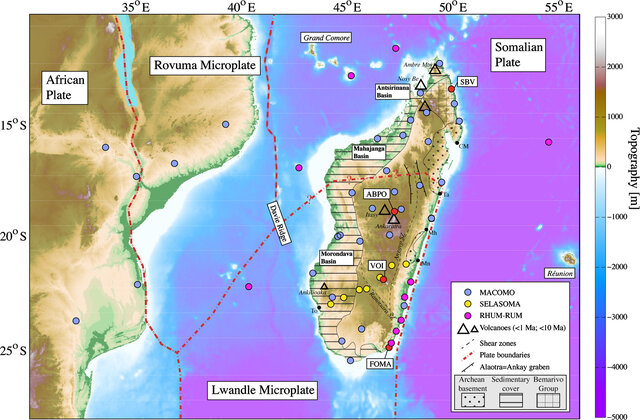
\includegraphics[width=0.5 \linewidth]{./Figures/TopologicMaps/geologyMadagascar.jpeg}
    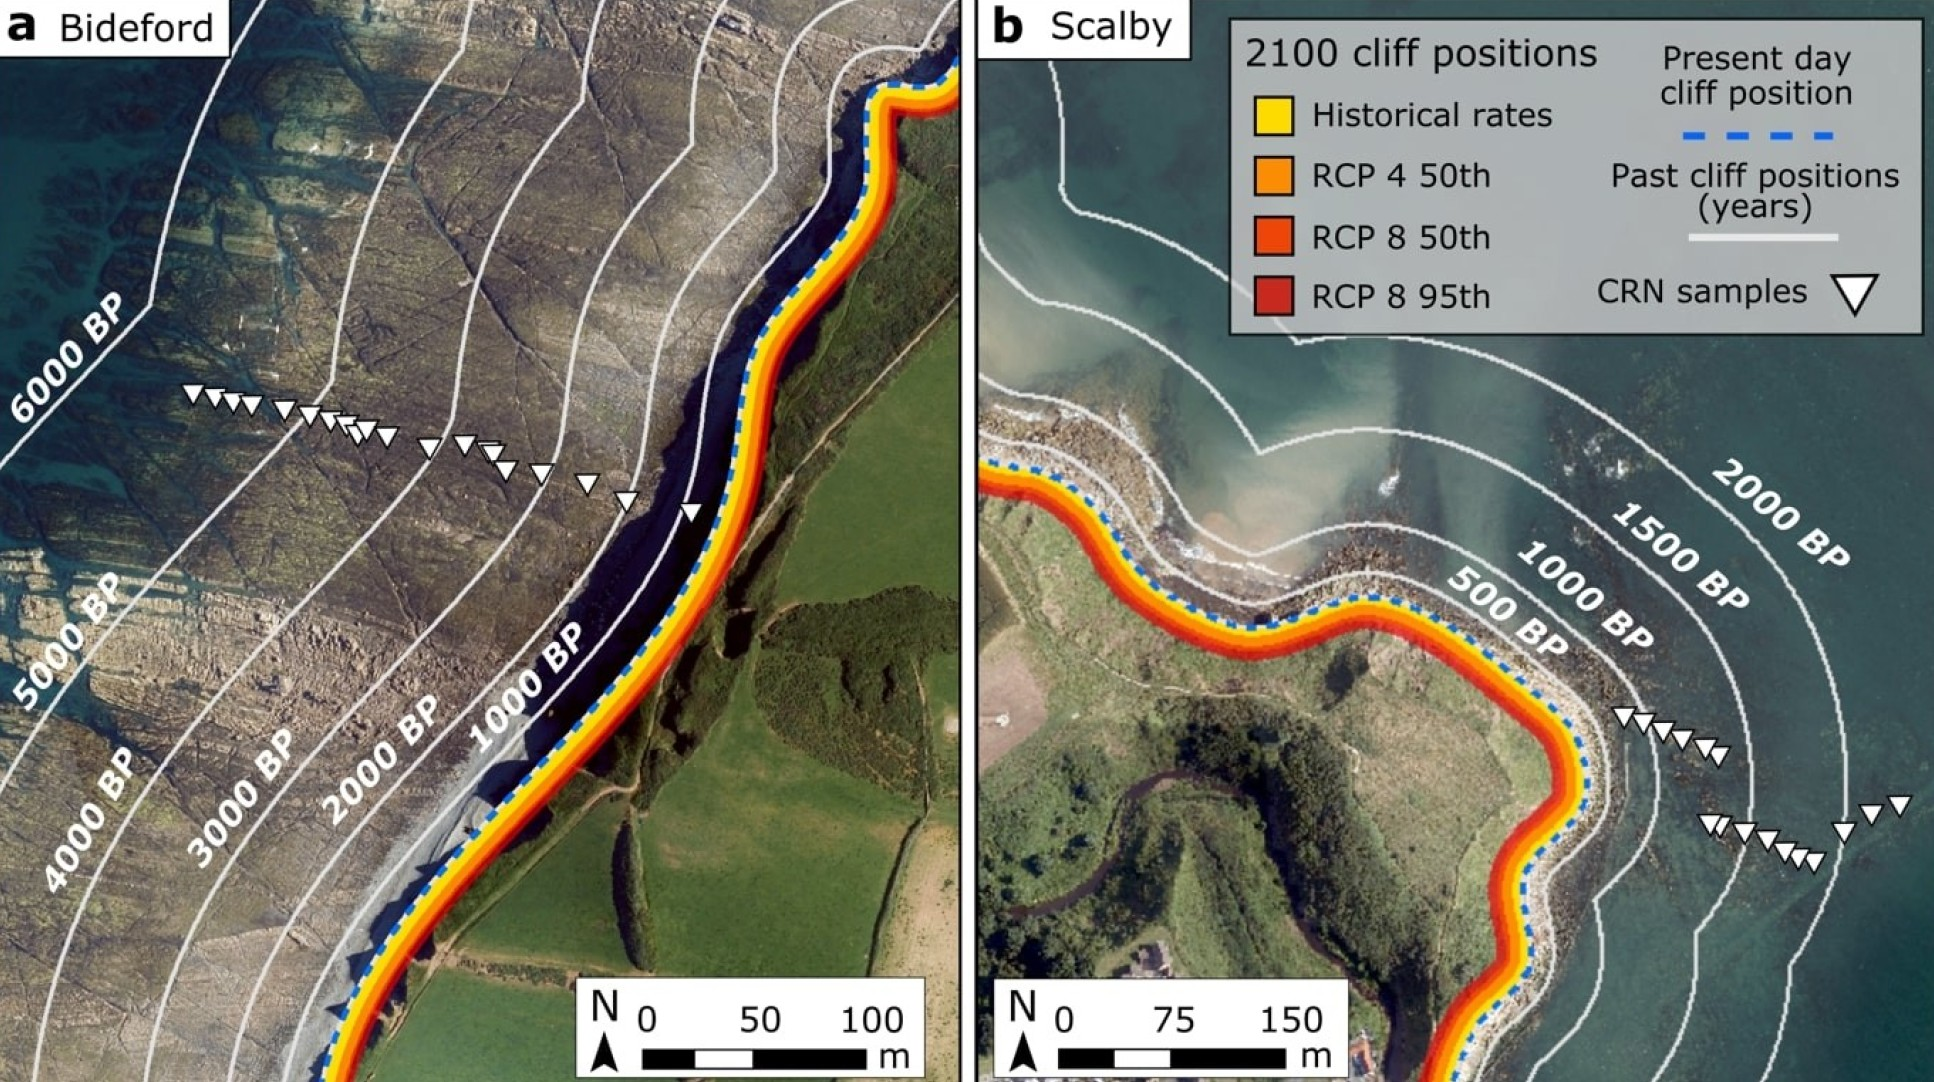
\includegraphics[width=0.5 \linewidth]{./Figures/TopologicMaps/CliffErosionBidefordAndScalby.jpg}
    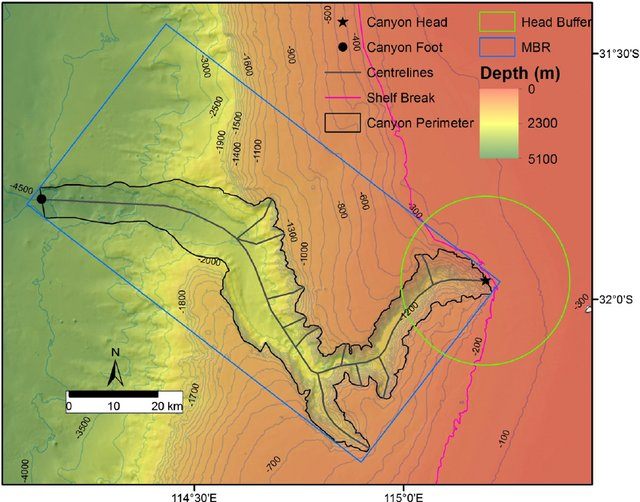
\includegraphics[width=0.5 \linewidth]{./Figures/TopologicMaps/PerthCanyon.jpg}
    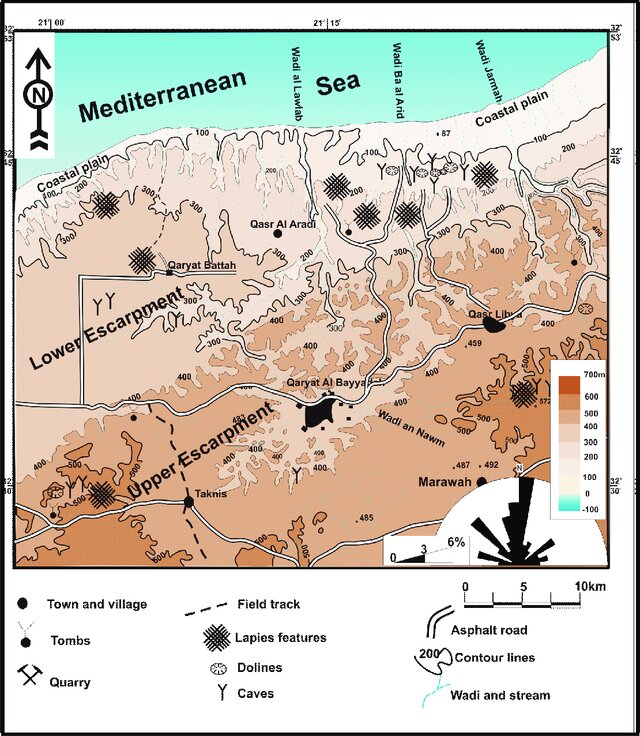
\includegraphics[width=0.5 \linewidth]{./Figures/TopologicMaps/QasrLibya.jpg}
    \caption{Four examples of topographic maps used in earth science. From left to right and top to bottom: Sedimentary distribution other Madagascar island \cite{Pratt2017}, evolution of coastlines at Bideford, UK and Scalby, UK over the last 6000 years and 2000 years respectively (BP = Before Present) \cite{Shadrick2022}, localization of key parameters of Perth Submarine Canyon, Autralia \cite{Huang2014}, and geological features distribution of karstic landscape at Qasr Lybia, Libya \cite{ElAmawy2009}}
    \label{fig:semantic-representation_presentation}
\end{figure}

% Slight introduction
Topographic maps are very useful tools for biologists, geologists or even oceanologists (which would call them "bathymetric charts"). These maps are displayed in 2D but provide 3D information about the altitude (or depth), but can also use symbology to represent the important elements that need to be visible. Map symbols are important in order to extract as much information as possible from a 2D object. In cartography, map symbols are defined as geometric primitives such as points, polylines, polygons, and (more rarely) polyhedrons. These symbols are a simplification of the content of an environment, or an abstraction of the 3D nature of the terrain features as we can see in the examples in \cref{fig:semantic-representation_presentation}. This is useful to understand the relationship between the different features, which may enable to deduce physical rules in the evolution of a terrain. 

% WHo would want it, and why?
In such way, geologists can study the distribution of peaks in a mountain range, the location of soil types in an area, which in turn allow to deduce possible locations of karst networks, for example. Using the same tools, a biologist may interpret the effect of natural or artificial reefs on coastal erosion, or understand more clearly the interactions inside an ecosystem. Oceanologists may also deduce, using the same strategy, the formation of canyons and fans from old river systems. [A REDIRE]

By simplifying the surface details in maps or models, we can concentrate more effectively on gaining a deep understanding of the underlying processes that shape the terrain. This focused understanding allows us to apply the insights we gain to a wide variety of terrain types. Essentially, this approach enables us to generalize our findings and apply them across diverse geographical landscapes, facilitating broader and more versatile applications of our knowledge.

Parallelly, terrain artists most of the time sketch the global shape of the terrain they will model beforehand, such that they can check, before the modeling part, that the consistency and plausibility of the terrain will be valid. Looking at a simplified map before starting the modeling step allows the designer to modify the overall shape of the terrain, at a large scale, before the 3D geometry comes into play, generating too much control points or vertices to be able to deal with.

Starting from an initial configuration or providing conditions on the desired output terrain, the algorithm we propose will let the different terrain features evolve as a multi-agent system in which the user can apply modifications or new constraints on the state of the environment. The resulting configuration is an environment conform to the constraints given by the user over the distribution of features present in the scene.

% Why it does not already exists?
As described in the previous chapter, most terrain generation algorithm use the geometry of an initial terrain surface to iteratively apply changes such as noise-based algorithms or erosion simulation. While the introduction of information about some environment variables or properties of the ground may influence the result of an algorithm, the control of the global shape of the terrain is lost as it treat locally the surface, without knowing which feature a certain point on the surface lies on.

% Personal motivation
The question which led to our solution is the multi-scale user interaction: "Is it possible to provide an interaction mean for terrain generation allowing the user to interact with a small structure like a rock in the same manner as with a large structure like a mountain?". 
In this work, we want the user to be able to have a large scale representation of the terrain in order to generate a landscape that satisfies his needs while keeping the possibility to apply large modifications.
In discussion with robotician users, we realise that we want to create a large landscape that can contain interesting configurations, select a smaller region that may have features in a disposition that fits its requirements and then refine again the given region.
In the optic of generating a large scale terrain in which we could focus the generation effort in a certain region, we wished to be able to see a coarse representation that can be computed quickly.

We aim for our terrain generation method to be versatile enough to handle both terrestrial and aquatic environments. This dual capability would allow the method to be applicable to landscapes above the water level, such as mountains and valleys, as well as to submerged terrains, such as oceanic canyons and coral landscapes.

Because many geographical terms and computer science terms are deceptive cognates, we will try to find middle ground in the naming of our introduced structures to avoid as much as possible any ambiguity between the research fields.
% Because many geographical terms would become ambiguous in computer science terms, in which this thesis lie in, we will translate some vocabulary in a way that may be disapproved by geologists, but we are doing our best to keep it as acceptable for each field as possible.


% \subsection{Nomenclature}
% % Geographical feature/entity -> Semantic Terrain Entity
% A geographical feature, also known as a feature, object, or entity, is a discrete phenomenon located at or near the Earth's surface, relevant in geography and geographic information science. It represents geographic information that can be depicted in maps, geographic information systems (GIS), and other forms of geographic discourse. The term "feature" includes both natural and human-made objects, ranging from tangible items like buildings to intangible concepts like neighborhoods. Features are distinct entities with defined boundaries, differentiating them from continuous geographic masses or processes occurring over time. They can be categorized as natural features, such as ecosystems, biomes, water bodies, and landforms, or artificial features, such as settlements, administrative regions, and engineered constructs. Geographic features are described by characteristics including identity, existence, classification, relationships with other features, location, attributes, and temporal aspects. Information about these features is stored in geographic databases using models like GIS datasets, which organize and represent these features in structured formats.
% % A geographical feature, also referred to as a feature, object, or entity, is a discrete phenomenon located at or near the Earth's surface, relevant in geography and geographic information science. It is an item of geographic information that can be represented in maps, geographic information systems (GIS), remote sensing imagery, statistics, and other forms of geographic discourse. The term "feature" is broad and inclusive, encompassing both natural and human-made objects. It includes tangible items like buildings as well as intangible concepts like neighborhoods. Features are discrete entities with distinct identities and locations, characterized by defined boundaries that differentiate them from other objects, distinguishing them from geographic processes, which occur over time, and geographic masses or fields, which are continuous. In geographic information science, "feature," "object," and "entity" are often used interchangeably, although some formal distinctions exist, such as seeing a feature as an abstraction of a real-world phenomenon. Geographical features can be categorized into natural and artificial types. Natural features include ecosystems, which are communities of organisms interacting with their environments; biomes, which are large areas with ecologically similar communities defined by plant structures, climate, and ecological patterns; water bodies, which are significant accumulations of water like oceans and lakes, either distinct or conceptual in nature; and landforms, which are physical structures such as mountains and valleys defined by surface form, location, and topography. Artificial features encompass settlements, which are human communities ranging from small villages to large cities, including infrastructure like roads and buildings; administrative regions, which are social constructs like states and neighborhoods used for organizational purposes; engineered constructs, which are man-made structures such as highways and airports; and cartographic features, which are abstract map representations, such as grid lines and boundaries, that do not physically exist. Geographic features are represented by descriptors of their characteristics, including identity, existence, kind, relationships, location, attributes, and time. Each feature is unique, often identified by names or codes, and its existence refers to its presence in the real world, including features that are proposed or planned. The kind refers to its classification, such as a building or river, while relationships describe spatial, meronomic (part-whole), and genealogical (parent-child) connections with other features. The location provides a description of where a feature is, including its shape and extent, and attributes describe other characteristics, such as population or size, often expressed as text or numbers. Time relates to the temporal aspects of a feature's characteristics, describing changes over time. Information about features is stored in geographic databases, often using vector data models, including GIS datasets, which help represent these features and their various descriptors in a structured format.

% % Field -> Environmental Attribute
% In geography, the term "field" refers to a continuous spatial phenomenon defined across a region, where each point in that region has a specific value of some variable. Unlike discrete objects, which have distinct boundaries and identities, fields represent variations of phenomena occurring over a continuous space, such as temperature, elevation, or precipitation. Fields can be either scalar or vector quantities: scalar fields represent a single value at every point, like temperature, humidity, or elevation, while vector fields represent quantities with both magnitude and direction, such as wind velocity or ocean currents. Examples of fields in geography include topographic fields, where elevation values are distributed across a landscape; climatic fields, where temperature or precipitation values are mapped over a geographic area; and magnetic fields, which capture the intensity and direction of magnetic forces at various points on the Earth's surface. Fields are often represented mathematically using functions or equations that define how the field's value varies over space, including interpolation or modeling techniques to estimate field values at unsampled locations. In Geographic Information Systems (GIS), fields are typically represented as raster data, where a grid of cells captures the continuous variation of a field across a landscape, with each cell holding a value representing the field's magnitude at that location. Fields are crucial for spatial analysis and modeling, allowing geographers to study patterns and processes that vary continuously across space, such as climate change, land surface modeling, and resource distribution. Thus, in geography, a field is a method of representing continuous spatial phenomena, enabling the analysis of patterns and trends across geographic spaces.

% % Event -> Geological Event
% In philosophy, an "event" is defined as an occurrence or happening that takes place at a specific time and location, characterized by its temporal nature and involvement in change or transition. Unlike static objects, events are dynamic and are often considered fundamental constituents of reality. They typically involve transformations from one state to another, such as a tree falling, and are central to discussions about causality, as they can serve as causes or effects within causal chains. Philosophers debate whether events are basic entities or reducible to other kinds of entities, like properties of objects or states of affairs. They also explore how events are individuated and identified, what distinguishes one event from another, and how events relate to objects. Linguistic and logical analyses focus on how events are described in language, often through verbs and predicates, and how they relate to entities involved. Various philosophical theories, such as process philosophy, emphasize events over static entities, offering different frameworks for understanding the nature of events and their role in the structure of reality. Overall, events are crucial for understanding change, causality, and our perception of the world.

% % Visualization

% \subsection{Features on field experts maps}
% - ... 
% \subsection{Topographic/Planimetric maps}
% - ... 

% \subsection{Analogy}
% - Compare our nomenclature with introduction \\
% - ... 

\section{State of the art}
\label{sec:semantic-representation_related-works}

\subsection{Vector modeling}
...
\subsubsection{Implicit modeling}
...
\subsubsection{Diffusion models}
...

\subsection{Ecosystems simulation}
...
\subsubsection{Environment modeling}
...
\subsubsection{Individual process}
...
\subsubsection{Multiple entity simulation process}
...
\subsubsection{Cellular automata}
...

Procedural terrain generation has been heavily studied for the last 40 years \cite{Galin2019}. Researches in this topic try to find new solutions to compromise between realism, user control and efficiency \cite{Gain2009}. Using fractal noise parametrized to resemble real landscape has been an important first step \cite{Musgrave1989} as it's a fast and light solution to generate procedurally the appearance of mountains. The lack of user control pushed newer works toward the use of controlled noise by including real DEM in the process through learning \cite{Kapp2020, Brosz2007}, while the rise of deep learning technologies gave higher control to the user through sketches \cite{Guerin2017, Talgorn2018}.

All the algorithms aim to reproduce plausible relief in terrestrial landscapes, mostly limited to alpine landscapes, but a lack of research can be found in almost all other biomes \cite{Smelik2014}. Underwater landscapes generation, for example, has been almost completely absent from literature for many reasons: the difficulty of accessing the area, the lack of visibility under water and the complex physics of underwater geology and biology make the algorithms adapted for this environment scarce. 

While stochastic noise can be sufficient to model coarsely the ocean floor \cite{Mareschal1989}, this process won't cover areas with the biggest biomass, near shallower waters such as near coasts and islands. These areas, that represent a very small portion of the oceanic surface, are much more complex as many interactions between biolife, air and water are in action.

Due to the impossibility to observe the large-scale and the small-scale of underwater environments, some works related to geology model large structures like the profile shape of the coral reef \cite{Bosscher1992}, simulate its surface growth \cite{Li2021}, or use procedural algorithms for single coral colonies' growth simulation \cite{Abela2015}. We however don't have a mix of the different scales, and neither methods take into account the environment such as the topography or the interaction of different terrain features. This is mainly due to the fact that the evolution time for each scale varies from a span of weeks to thousands of years.

Recent works have been presenting "feature tools" to correct landscapes from unaccurate DEM (2.5D) using vector-based features that modifies the geometry of the ground and water bodies to fit thir respective 2D satellite images, by explicitely defining the position of natural features like rivers and mountains \cite{Ketabchi2016}. Visible 3D features like vegetation and buildings can also be added in the final result as meshes affected to a single point. This leads to sketch-based applications where features are represented like topographic maps. This solution allows for the manipulation of an existing terrain, guided by a real-world satellite image, but lacks the possibility to completely generate an unseen landscape or for the terrain features to interact between them. Feature tools have been proposed to generate terrains from scratch \cite{Smelik2010a}, but usually require to define in advance the interactions between each feature like a automatically displaying a bridge when a river crosses a road.

In an ecosystem, every element within the system has an impact on its surroundings, and accurately simulating physical properties like shading, heat, and humidity can require immense computational power. To address this, instead of simulating these properties individually for each object, they can be represented as scalar fields that span the entire scene. These scalar fields, which may represent temperature, humidity, or occlusion, are locally influenced by nearby objects and terrain features, such as trees casting shadows or buildings radiating heat. This approach, as described in \cite{Grosbellet2016, Guerin2016a}, allows for the environment's physical properties to be computed in a more efficient manner. By simplifying the complex interactions into these localized scalar fields, they called environmental objects, their method provides a scalable system that can handle large and detailed scenes. This system effectively renders scene details, such as snow accumulation or leaf distribution, in a way that is visually plausible, ensuring realistic results without the need for exhaustive simulations. 
%In a similar way, other works represent the wind flow as a composition of local vector fields \cite{Wejchert1991}, avoiding complex fluid simulation while providing user control in a lightweight model. We extend these works by incorporating a time-evolution system such that the scene can be dynamic.
In a similar approach, parallely Wejchert and Haumann \cite{Wejchert1991} and Sims \cite{Sims1990} represent wind flow as a composition of local vector fields, known as "flow primitives", which can be combined to simulate complex fluid behavior. This method simplifies the computation by avoiding full fluid simulations, instead offering a lightweight model that allows for intuitive user control over the flow dynamics.
By combining these approaches, we can create dynamic ecosystems where environmental effects and fluid flows interact in a plausible manner, while requiring a low computation effort and preserving a high user control.


\section{Description of the method}
\label{sec:semantic-representation_pipeline}

In this section, we present the pipeline and processes that underpin our method. Our approach introduces the concept of \glosses{EnvObj}, simplified terrain features that interact with their surroundings to simulate complex ecosystem dynamics. These \glosses{EnvObj}, which can represent natural features such as trees, rivers, or rocks, influence and are influenced by scalar fields like temperature, humidity, and elevation. The method is structured into several key phases: initialization, where the foundational elements of the terrain and \glosses{EnvObj} are set up; an iterative generation process, where these \glosses{EnvObj} are instantiated and interact with their environment; and finally, the production of a sparse representation of the scene's features. This section details each of these phases, explaining how the system dynamically adapts to user input and environmental changes.

\subsection{Pipeline}

\begin{figure*}
    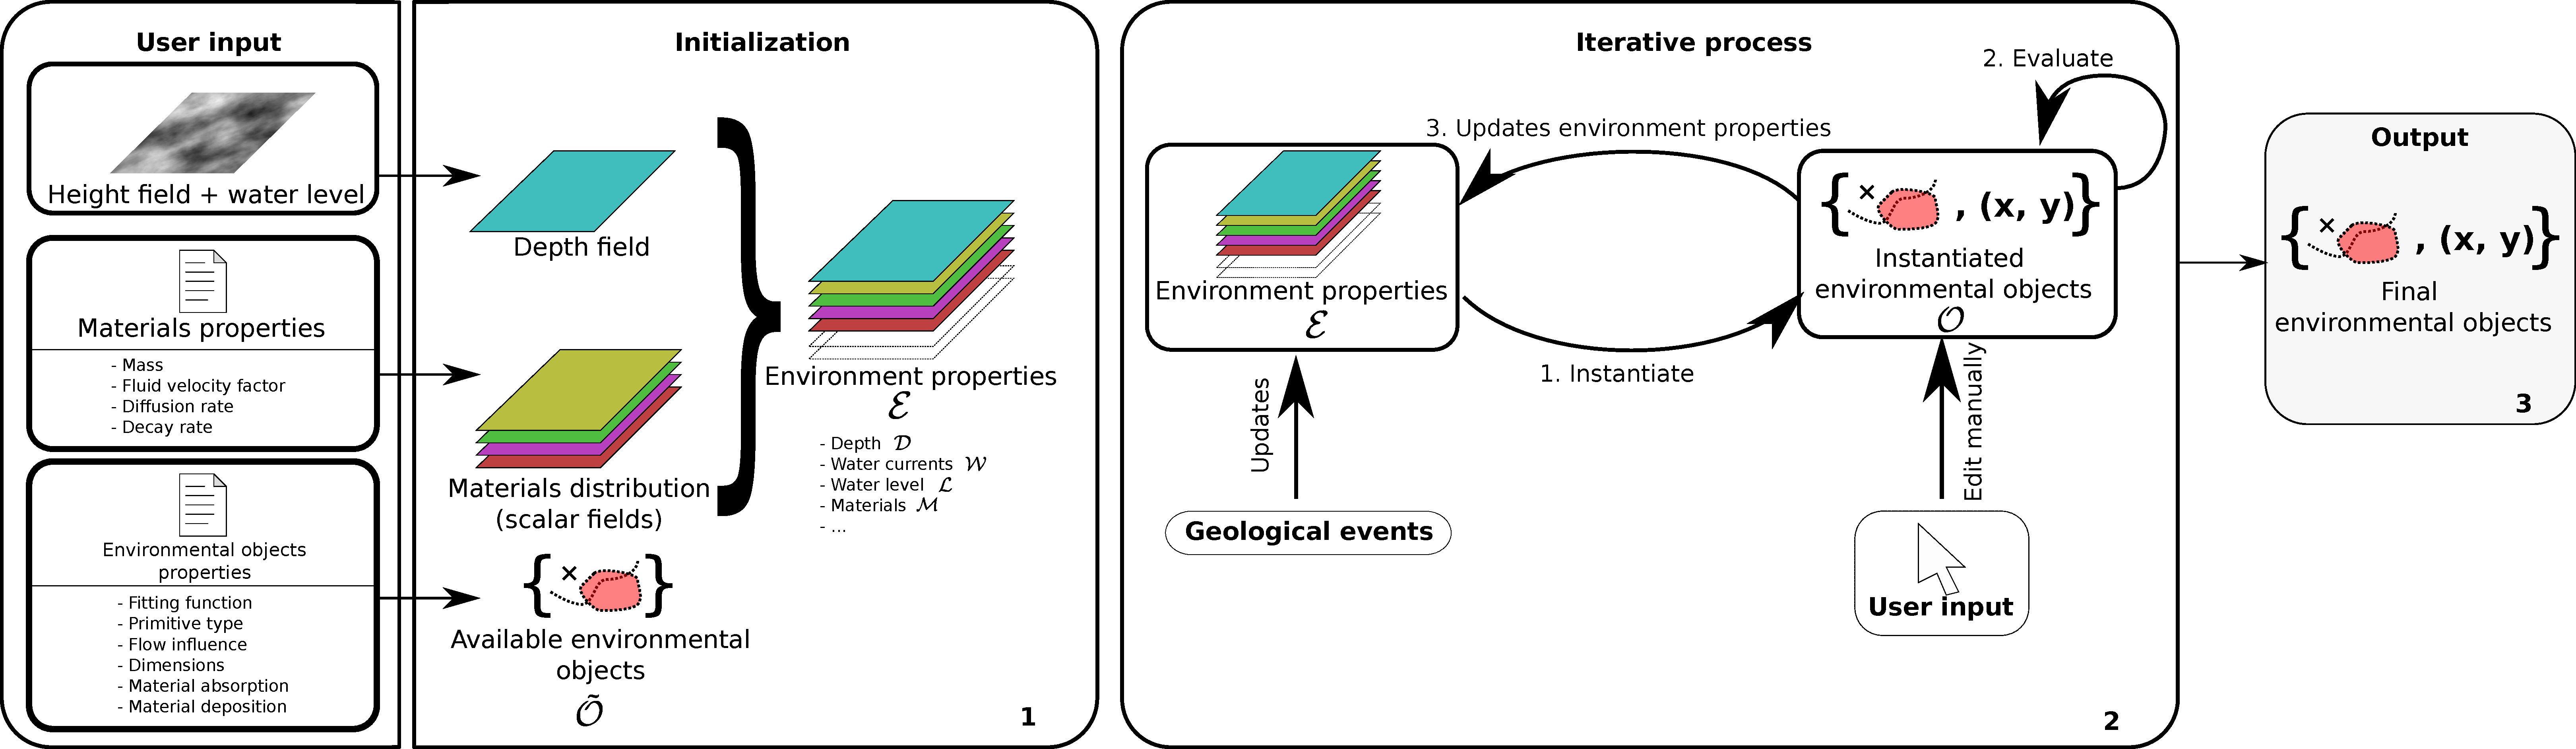
\includegraphics{Figures/pipeline.pdf}
    \caption{Overview of the pipeline of the method. The user provides as input an initial height field and sets the water level, as well as a definition of the \glosses{EnvMat} properties and \glosses{EnvObj} properties that will be used in the iterative process. These inputs are initialized as an initial set of \glosses{EnvObj} and scalar fields that represents the \glosses{EnvVal}. In the iterative loop, new \glosses{EnvObj} are instantiated using the current state of the environment at their optimal position. The existing \glosses{EnvObj} in the terrain reevaluate their \gloss{FitnessFunc} to grow or die and update the \glosses{EnvVal} locally. At each iteration, \glosses{GeoEvent} can update the \glosses{EnvVal}, while the user can interact directly with the \glosses{EnvObj}. The result of the whole process is a set of \glosses{EnvObj} which is a sparse representation of the features of the scene. }
    \label{fig:semantic-representation_pipeline}
\end{figure*}

\subsubsection{Initialization}

The generation of the terrain is initialized using an initial height field $h$ and an initial water level $\Wlevel$. 
During this chapter we will include many features depending on altitude or depth, so we will use the shorthand notations $\height = h - \Wlevel$ and $\depth = -\height$. The height field provides variation on the altitude, which can influence the generation process of the scene.

The list of available \glosses{EnvObj} $\availableObjects$, representing the different features that can be present in the scene, are provided with their properties: type, size, \glosses{GenRule} and effects on the \glosses{EnvVal} (\cref{sec:semantic-representation_environmental-objects}). A target list of \glosses{EnvObj} $\targetObjects$ can be defined to control the final result of the generation.

Finally, different \glosses{EnvMat} are defined with their properties such as diffusion speed, mass, decay rate and influence from the water currents. An initial environment configuration resulting from the initial height field $\height$ and water level $\Wlevel$, the \glosses{EnvMat} distribution $\material$ (represented as scalar fields $\material: \R^2 \to \R$) and water currents $\Water$ (as a vector field $\Water: \R^2 \to \R^2$) will be used by the \glosses{EnvObj} of the scene to simulate their growth and spawn at the most probable position. The \glosses{EnvVal} are noted $\environment = (\depth, \Water, \Wlevel, \material)$ (\cref{sec:semantic-representation_communication}).

The definition of \glosses{EnvObj}' properties and \glosses{EnvVal} is done with field experts, providing the pertinent parameters required to model the evolution of the terrain features using expert knowledge (\cref{sec:semantic-representation_biology}). 

The generation phase starts with an initial set of \glosses{EnvObj} present in the scene, which can optionally be pre-filled.

\subsubsection{Generation process} 

%- Main loop
Once the initialization phase is done, the generation begins. The generation process is incremental and its main loop is composed of two different steps: the instantiation of new \glosses{EnvObj} then the update of the environment. This loop is repeated until the user is satisfied with the look of his environment or following rules like a number of features threshold or a targeted list of \glosses{EnvObj} as described in the layout planner defined in \citep{Tutenel2009}.


\subsubsubsection{Instantiation}
% - Object instantiation
At each iteration, new \glosses{EnvObj} can be created at their most fitting locations if possible. The \glosses{GenRule} provided in the initialization phase are used to find an optimal position from stochastic sampling (\cref{sec:semantic-representation_generation-rules}). 
All \glosses{EnvObj} are evaluating their state analytically using a \gloss{FitnessFunc} and a \gloss{FittingFunc} provided as input (\cref{sec:semantic-representation_generation-rules}).

\subsubsubsection{Environment update}
% Once the new objects are instantiated, the process can continue.
% - Environment update
Once the instantiation step is done, the \glosses{EnvVal} are updated by each \gloss{EnvObj} through \glosses{EnvModif}, which depose and absorb some of the \glosses{EnvMat} $\material$ (\cref{sec:semantic-representation_materials}) while modifying the water currents $\Water$ (\cref{sec:semantic-representation_water-currents}) and the height field $\height$ around them. Finally, water currents and terrain slope displace \glosses{EnvMat} of the terrain until reaching a dynamic equilibrium in the environment at each iteration.

% We consider the water currents to be a steady-state flow, allowing us to remove the variation from time in the flow equations.
% The water currents are updated locally by each \gloss{EnvObj} using an analytical form $W^*(\p) = W(\p) + \omega(\p)$.
During the generation process, the user can alter directly the distribution and shapes of the \glosses{EnvObj} (\cref{sec:semantic-representation_manual-interaction}) and perturb the generation process by planning \glosses{GeoEvent} that have impacts on the \glosses{EnvVal} (\cref{sec:semantic-representation_events}).


\subsubsection{Output}
% - Output result
The output of our system is a set of \glosses{EnvObj} disposed in the plane. We do not provide the 3D representation of the \glosses{EnvObj} in this chapter, letting the user define the rendering method. The figures used in the chapter use a mix of implicit surfaces and triangular meshes.

\subsection{\Glosses{EnvObj} $\objects$}
\label{sec:semantic-representation_environmental-objects}
A geographical feature, also called object or entity, is defined as a discrete phenomenon located at or near the Earth's surface, relevant in geography and geographic information science (GIScience). It represents geographic information that can be depicted in maps, geographic information systems (GIS), and other forms of geographic media. This term includes both natural and human-made objects, ranging from tangible items like buildings or trees to intangible concepts like neighborhoods or savana. Features are distinct entities with defined boundaries, differentiating them from continuous geographic masses or processes occurring over time. They can be categorized as natural features, such as ecosystems, biomes, water bodies, and landforms, or artificial features, such as settlements, administrative regions, and engineered constructs. Geographic features are described by characteristics including identity, existence, classification, relationships with other features, location, attributes, and temporal aspects. Information about these features is stored in geographic databases using models like GIS datasets, which organize and represent these features in structured formats. As the term "feature" is overused in computer science, we will use the term \gloss{EnvObj} in this work.

Each \gloss{EnvObj} is shaped with a simple geometric shape called a "skeleton" that defines where it is located and how it fits into the environment. The \gloss{Skeleton} can either be, as used in cartography, a point, a curve or a region. We will then refer to our \glosses{EnvObj} as point-based, curve-based or region-based, respectively.  
These \glosses{EnvObj} interact with the environment $\environment$ by changing local conditions using the \glosses{EnvModif}. For example, the presence of a river might increase the moisture in the surrounding area, while a mountain might induce more rockiness in the soil composition. They can also absorb changes from the environment, such as a forest taking in humidity from the air.
The placement of \gloss{EnvObj} is determined by a \gloss{FitnessFunc} $\fitnessFunc$, which evaluates how suitable a location is based on the \glosses{EnvVal}. Once a suitable location is found, the \gloss{FittingFunc} optimizes the shape and position of the entity to fit as best as possible into the environment $\fittingFunc$.

%This approach allows us to "spawn" new entities based on rough altitude estimates, ensuring that their placement is contextually appropriate while deferring the detailed computation of their final shape to a later stage, if required by the user.
% The coarse height function thus acts as a middle between the semantic modeling of terrain and the precise 3D modeling. It provides enough information to make informed decisions about \glosses{EnvObj} placement and \glosses{EnvMat} while preserving the flexibility to integrate more detailed modeling techniques. This method ensures that the terrain generation remains interactive and scalable, allowing for the dynamic and realistic placement of entities in complex landscapes without being tied to the immediate computation of detailed topography.

% \Glosses{EnvObj} are rule-based objects following rules depending on their local environment for evaluation their state in their life cycle. We can see them as a life form in the way that they are created and eroded with time. During their lifetime, they influence their local environment by depositing and absorbing \glosses{EnvMat} around them and influencing the water currents. The environment objects are described spatially as a single point, a parametric curve or a region.


\subsection{\Glosses{EnvVal} $\environment$}
\label{sec:semantic-representation_communication}

In geography, a "field" refers to a continuous spatial phenomenon across a region where each point has a specific value of a variable, unlike discrete objects with distinct boundaries. Fields can be scalar, representing a single value at every point (like temperature or elevation), or vector, representing quantities with magnitude and direction (like wind velocity). Examples include topographic fields for elevation, climatic fields for temperature or precipitation, and magnetic fields for magnetic forces. Because of the ambiguous nature of the term "field" with mathematics and computer science, we will define the geographic fields as \gloss{EnvVal}.

In an ecosystem simulation, each actor of the ecosystem has an impact on all other actors, which results in an exponentially growing computation effort as the number of elements of the terrain increase. We avoid this problem by considering the \glosses{EnvVal} as a proxy to allow any \gloss{EnvObj} to interact with any other one. Each of the \gloss{EnvObj} have a local impact on the \glosses{EnvVal} without knowledge of neighboring \glosses{EnvObj}. This modification of the \glosses{EnvVal} are presented as the effect of \glosses{EnvModif} defined for each \gloss{EnvObj}. % can be due to an absorption and deposition of some material $\material$ or an influence on the water currents.

In this work, we have integrated vector \glosses{EnvVal} (e.g., water currents $\Water$) and scalar \glosses{EnvVal} (e.g., altitude $\height$, water level $\Wlevel$, and various material properties $\material$) under the unified term "environment," denoted as $\environment = \left( \height, \Water, \Wlevel, \material \right)$. The \glosses{EnvMat} represent abstract quantities such as the availability of sand, salt, moisture, or rocks at each point. It is important to emphasize that these materials are not to be visualized as physical layers stacked on the terrain surface. Instead, they should be understood as conceptual resource distributions that influence the environment and the behavior of \glosses{EnvObj}, rather than as something directly observable in the scene.

\subsubsection{\Glosses{EnvModif} $\environmentModif$}
The environment determine if a \gloss{EnvObj} does belong at a certain position. When a \gloss{EnvObj} is placed, its surrounding \glosses{EnvVal} can be affected though \glosses{EnvModif} noted $\environmentModif = (\heightModif, \waterModif, \nothing, \materialModif)$ defining a change of height $\heightModif$, changes in the water currents $\waterModif$ and \gloss{EnvMat} alteration $\materialModif$. 

\Glosses{EnvObj} are subject to altitude conditions. However, to maintain a clear distinction between semantic modeling and 3D modeling, we do not compute the exact physical shape or detailed height field of each \gloss{EnvObj}. Instead, we define a \gloss{CoarseHeight}, a parametric representation derived from the \gloss{Skeleton} to provide a rough estimate of the changes in elevation around it. This simplified model of how the \gloss{EnvObj} influences the surrounding terrain's altitude allows us to cheaply evaluate the potential presence of new entities that have altitude-dependent conditions without the need to perform expensive computations to generate a detailed height map of the entire terrain. 

Altering the vector field of the water currents $\Water$ is done by the composition of the effect $\waterModif$ of each object at a position $\p$ as introduced in \citep{Wejchert1991}, while we use the formulation of Kelvinlets \cite{DeGoes2017} in the computation of effect of each \gloss{EnvObj}.

Each \gloss{EnvObj} has intrinsic \glosses{EnvMat} that can be seen as "spreading" and "absorbed" around its skeleton over time. A coral reef may produce coral polyps and at the same time reduce the water currents. It grows thanks to the deposition of limestone from coral colonies. In our model, the colonies affect the \glosses{EnvVal} through the deposition of \gloss{EnvMat} $\materialModif_\text{limestone}$, which in turn, is absorbed by the coral reef, without a direct exchange between the two \glosses{EnvObj}.

The alteration of a scalar \gloss{EnvVal} is done by adding or removing some amount around the \gloss{Skeleton} of the \gloss{EnvObj} and diffusing it in the space, influenced by the water currents. We consider the system to be \gloss{SteadyState}, garantied by the introduction of a decay rate $\decay > 0$ in the computation of the diffusion and advection.



\section{Placement of \glosses{EnvObj} in an environment}
\label{sec:semantic-representation_generation-rules}

At each iteration of our algorithm, we want our \glosses{EnvObj} to be at plausible positions. We do not guaranty a temporal continuity between iterations as in \citep{Ecormier-Nocca2021}, so the objective is to add new \gloss{EnvObj} in order to satisfy the users wishes, while conserving the plausibility of the scene. Rather than "forming" these \glosses{EnvObj}, our method "reveals" them, much like a paleontologist uncovers fossils during an excavation. A paleontologist does not dig randomly across the Earth to find fossils; instead, they analyze the geological context to identify the most likely locations. Similarly, our method observes the environment and estimates where certain elements are likely to exist. For example, in hydrology, if a river appears to originate from nowhere, it might suggest the presence of a karstic river system upstream. In urban planning, if many roads converge at a certain point, it is reasonable to expect that a city is located there. This approach ensures that Semantic Terrain Entities are revealed in positions that are contextually appropriate and coherent within the landscape.

We will follow the same intuition using a \gloss{FitnessFunc} for each of the \gloss{EnvObj} that may be spawn in the terrain. The \gloss{FitnessFunc} defined $\fitnessFunc: \environment \to \R$ provides a score indicating how well the \gloss{EnvObj} may fit in this position. Evaluating this function at multiple position results in an approximation of the fitness map of the entity. Once the most probable position is found, we can find the most plausible shape of the \gloss{EnvObj} using the \gloss{FittingFunc} $\fittingFunc$.

For this task, we place a new elements required at the most plausible position using the analysis of the \gloss{FitnessFunc} of each \gloss{EnvObj}. We know that each \gloss{EnvObj} will modify the environment surrounding, which may make previously instantiated \glosses{EnvObj} unfitted. Knowing this,the goal is to add the new element at the position that will change the least the stability of the system. 

Genetic algorithms or Depth First Search algorithms could be used to try many possibilities until a local or global minimum could be found, but this would require a large processing power. Naive genetic algorithms would place a \gloss{EnvObj} at a certain position at each iteration and evaluate the stability of the environment, repreating this operation while varying slightly the position of the \glosses{EnvObj} or the type of \gloss{EnvObj} instantiated at each iteration, resulting in way too much computation to stay interactive. The Depth First Seach algorithms would require to compute all the possible combinations of \glosses{EnvObj} and positions which, given the fact that we want a continuous position in order to work multi-scale, would require to compute an incredibly high amount of possible configurations in order to find a plausible situation, on average. We will work with an evolutionary algorithm to find a compromise between fast computation and a satisfying result.

Our placing algorithm is done in two steps: first, it identifies the global location where a \gloss{EnvObj} best fits within the environment $\environment$ using its \gloss{FitnessFunc} $\fitnessFunc$, which evaluates the suitability of each point $\p$ based on the \glosses{EnvVal} $\environment_p$, including factors such as altitude $\height(\p)$, water current velocity and direction $\Water(\p)$, water level $\Wlevel(\p)$, and the availability of \gloss{EnvMat} $\material(\p)$. Second, once the most suitable location is identified, the algorithm determines the most plausible shape of the \gloss{EnvObj} using the \gloss{FittingFunc} $\fittingFunc$.

To ease the reading the functions $\fitnessFunc(\environment(\p))$ and $\fittingFunc(\environment(\p))$ with $\environment(\p)$ the \glosses{EnvVal} at the point $\p$ of the terrain are simplified to $\fitnessFunc(\p)$ and $\fittingFunc(\p)$ respectively.

% Our placing algorithm is done in two steps: first we estimate at which global location the \gloss{EnvObj} fits the most given an environment $\environment$ using its \gloss{FitnessFunc} $\fitnessFunc$, secondly we estimate the shape of the skeleton of this \gloss{EnvObj} should take given a \gloss{FittingFunc} $\fittingFunc$.

% \Glosses{GenRule} provides, for each \gloss{EnvObj}, a \gloss{FitnessFunc} $\fitnessFunc$ defining the most probable location for an \gloss{EnvObj} to be found. \Glosses{FitnessFunc}' parameters contains, for every point $\p$, the \glosses{EnvVal} $\environment_p$ (the altitude $\height(\p)$, the velocity and direction of the water currents $\Water(\p)$, the water level $\Wlevel(\p)$ and the amount of each \gloss{EnvMat} available $\material(\p)$).

\subsection{\Gloss{FitnessFunc} $\fitnessFunc$}
"Darwinian fitness" refers to an organism's ability to survive and reproduce in its environment. It is a measure of how well-suited an organism is to its surroundings, and those with higher fitness are more likely to pass on their genes to the next generation. In a similar vein, the \gloss{FitnessFunc} of a \gloss{EnvObj} evaluates its suitability at a location in the terrain, extending the meaning to living features like forests and corals and non-living elements such as rivers, mountains, karsts, etc.

The fitness function is constructed by evaluating several environmental variables at a given location $\p$. These include altitude ($\height(\p)$) and its gradient ($\nabla \height(\p)$), the availability and gradient of various materials ($\material_i(\p)$ and $\nabla \material_i(\p)$), water current characteristics ($\Water(\p)$), and water level ($\Wlevel(\p)$). Altitude and its gradient can influence the placement of objects like rivers, which may prefer lower elevations, or forests, which might thrive on slopes. Each material, such as limestone, sand, or clay, is considered separately, and their availability and gradients at a location are crucial for determining the suitability of different \glosses{EnvObj}, such as a coral reef requiring specific substrates. The velocity and direction of water currents are essential for placing aquatic features or determining where erosion might occur, while the proximity to water influences the likelihood of placing wetlands, lakes, or other hydrological features.

These environmental variables are typically combined in the fitness function, often expressed as a weighted sum, but not restricted to this form:

\begin{align*}
    \fitnessFunc(\p) = w_1 \cdot \height(\p) + w_2 \cdot \nabla \height(\p) + \sum_{i} \left( w_{3,i} \cdot \material_i(\p) + w_{4,i} \cdot \nabla \material_i(\p) \right) + w_5 \cdot \Water(\p) + w_6 \cdot \Wlevel(\p)
\end{align*}

Here, $w_1, w_2, w_{3,i}, w_{4,i}, w_5, w_6$ are weights that reflect the relative importance of each factor for the specific \gloss{EnvObj} being considered.

Different types of \glosses{EnvObj} require different criteria for their fitness evaluation. For example, a river might prioritize lower altitude and proximity to water currents, while a forest might prioritize higher altitude and specific material availability. The flexibility of the fitness function allows it to be customized for each \gloss{EnvObj}, ensuring that the generated terrain remains coherent and realistic.

\subsection{\Gloss{FittingFunc} $\fittingFunc$}
The seed point of a spawning \gloss{EnvObj} is defined at the point $\p$ satisfying $\arg \max_\p \fitnessFunc(\p) $.
% a stochastic sampling of the plane. We propose different optimization means to find the optimal fitting position, depending on the \gloss{EnvObj} shape.

\subsubsection{Point-based \gloss{Skeleton}}
The spawning position of a punctual \gloss{EnvObj} is found at the local maxima of the \gloss{FittingFunc} from the seed point. While the \gloss{FittingFunc} doesn't have to be identical to the \gloss{FitnessFunc}, we usually use $\fittingFunc = \fitnessFunc$ for point-based \glosses{EnvObj}. If the two functions are different, the optimisation process simply follows the field's gradient $\nabla \fittingFunc$ until the local maxima is reached.

\subsubsection{Curve-based \gloss{Skeleton}}
% A curve can have different \glosses{GenRule}, making the definition of the functions easier depending if the \gloss{EnvObj}'s \gloss{Skeleton} has a notion of direction. It can either:
% \begin{itemize}
%     \item follow the gradient of the \gloss{FittingFunc} $\nabla \fittingFunc$, useful when the direction of the \gloss{Skeleton} has an importance like a river that has to run downhill,
%     % \item follow the isocontour $\nabla \fittingFunc^\perp$, [WAIT, IS THAT NEEDED?]
%     \item or optimize the energy of the function over its curve, like a coral reef that has to cover as much coral colonies as possible. % follow the heat points.
% \end{itemize}

% \subsubsubsection{Following the gradient}
% Following the gradient of the \gloss{FittingFunc} $\nabla \fittingFunc$ is done by extending a curve from the seed point towards $\nabla \fittingFunc$ until reaching a local maximum while also following $-\nabla \fittingFunc$ until finding a local minimum. We stop the building process when our curve reaches a length limit $\Length$. 

% This \gloss{FittingFunc} strategy is efficient to describe rivers as we can set $\fittingFunc(\p) = \height(\p)$ to force it to always run downstream. 

% \subsubsubsection{Energy optimization}
The skeleton of a curve-based \gloss{EnvObj} is determined by the shape that fits the most given the environment it is added to. 
Using a modified version the Active Contours algorithm \cite{Kass1988}, we can minimize the energy $\energy$ for the parametric curve $\curve$ given $\energy(\curve) = \Einternal + \Eexternal + \Eshape + \Egradient$ with  
\begin{align}
    \label{eq:internal-energy-equation}
    \Einternal &= \Ainternal \left( \int_{\curve}{ \norm{\curve'(s)}^2 \, ds} + \int_{\curve}{ \norm{\curve''(s)}^2 \, ds}  \right) \\
    \Eexternal &= \Aexternal \int_{\curve}{ \fittingFunc(\curve(s)) \, ds } \\
    \Eshape    &= \Ashape \left( \Length - \int_{\curve}{ \, ds } \right)^2 \\
    \Egradient &= \Agradient \int_{C}{ \dot{C'(s)}{\Delta \fittingFunc(C(s))} \, ds }
\end{align}
In this configuration, $\Einternal$ induce a smooth continuity of the curve by reducing the spacing of each point while reducing the curvature. Another energy, $\Eexternal$ integrate the \gloss{FittingFunc} over the curve, often seen as an attractor of the points, that tries to descent the gradient to find local minima. At the same time, $\Eshape$ apply constraints on the curve shape, which, in this case, is to target a specific length $\Length$. As such, the curve search for an optimized shape given constraints in $\Eshape$ for minimizing $\Eexternal$. We introduced a new term $\Egradient$ in the energy computation that push the points of the curve in the direction of the slope of the \gloss{FittingFunc}, also providing an orientation for the curve.

If a steep coast can be found where the terrain slope is important near the water level, we can define $\fittingFunc = \abs{\height + 1} / \norm{\Delta \height}$, but no orientation is needed, thus we set $\Agradient = 0$. In this case, the curve will follow a path at the water level and spread its extremities over areas with a steep slope. A river may also be symbolized as a parametric curve, but we need to add information about the direction and magnitude of the slope.  As such, we can use $\fittingFunc = \height$ which forces the direction of the curve to fit with the terrain slope. The introduction of the gradient component provides also an orientation to shapes.

\subsubsubsection{Internal energy}
The internal energy, already introduced in \citep{Kass1988} is composed of two components imposing penalities on the local properties of the points of the curve. The first derivative forces the points along the curve to be evenly spaced by minimizing the curve tension, while the second derivative restrict it from forming sharp corners. As our aim is to represent natural elements, we rarely find sharp elements and thus, keep the original definition from the Snake formulation.

\subsubsubsection{External energy}
The external energy is also present in the original work. Using an external scalar field, each point of the curve is forced to follow the steepest slope of the field. The external field can be seen as an attractor for the curve.

\subsubsubsection{Shape energy}
We introduced the shape energy, an energy defined on the whole curve to apply constraints on its final shape. As many natural features have a given dimension, we may add a constraint on the lenght of the \gloss{Skeleton}. 

\subsubsubsection{Gradient energy}
In our application, having information about the orientation of \glosses{EnvObj} may be essential. For this purpose, we introduced a gradient energy component in the formulation. The equation impose that the direction of the curve at any point should be directed towards the gradient of the scalar field. As the external energy pushes points toward the lowest point of the scalar field, the gradient field restrict the gradient descent for the global curve into a specific way, which may feel more natural.

During the optimization process, the gradient of the scalar field is already evaluated by the external energy optimization, so the addition of the gradient component is almost free.

% \subsubsubsection{Position constraint}
% As the curve minimize its energy, it may fly far away from the initial seed point. We added a last constraint about the positioning of the curve such that the distance between t

% The internal energy $\Einternal$ force the shape continuity while the shape energy $\Eshape$ force the shape into a specific target length $\Length$, and finally $\Eimage$ that use the definition of the \gloss{FittingFunc} to attract the points of the curve toward a local minimum.

% While the first two possibilities are trivial, the later can also be optimized using the Active Contours algorithm by optimizing the energy $\energy = \Einternal + \Eshape$ with \eqref{eq:internal-energy-equation}. We applied a length constraint on the curves : 
% \begin{align*}
%     \Eshape = \left( \Length - \length \right)^2
% \end{align*}
% with $\length$ the curve's length and $\Length$ the target length. This algorithm is sensible to the initial shape of the curve, so we start with a straight line following the isolevel at the seed point.

\subsubsection{Region-based \gloss{Skeleton}}

Region-based \glosses{EnvObj} follows the same process than curve-based \glosses{EnvObj} to define their \gloss{Skeleton}, at the exception of the gradient energy $\Egradient$ which have null value on closed shapes. 

The resulting energy $\energy$ to minimize for a closed region whose borders are defined by the curve $\curve$ can then be expressed as $\energy(\curve) = \Einternal + \Eexternal + \Eshape$.

The internal energy is expressed identically as for curve-based \glosses{EnvObj}. The extenal energy however, has to be modified to take into account the interior of the region instead of only the borders. We will use the idea of the Chan-Vese algorithm, differentiating the energy value for the inside $\domain$ and the borders $\curve$ of the region \cite{Chan2001, Getreuer2012}.

By adding a factor for the inside $\lambda_1$ and a factor for the borders $\lambda_2$, we can add weight depending on the required optimization. We can then define the external energy component $\Eexternal$ as:
\begin{align}
    \Eexternal = \lambda_1 \int_{\domain}{ \fittingFunc(s) \, ds } + \lambda_2 \int_{\curve}{ \fittingFunc(\curve(s)) \, ds }
\end{align}
We see that the definition of the energy formulation of the curve-based \glosses{EnvObj} is a specialization of the region-based, with $\lambda_1 = 0$ and $\lambda_2 = \Aexternal$

The use of external forces on the \gloss{Skeleton} can be useful as some landscape features are easier to define by what they contain, while other by what they separate. For example, a lagoon is formed by coral reefs surrounding it, while a forest is formed by the climatic conditions inside it that are propice for trees. A lagoon may then be defined with $\lambda_1 = 0$ and $\fittingFunc_{\text{lagoon}} = -\material_{\text{coral limestone}}$ while a forest sets $\lambda_2 = 0$ and $\fittingFunc_{\text{forest}} = -\material_{\text{humidity}} + \material_{\text{shade}} + \abs{\material_{temperature} - 10}^2$.

Finally, the shape constraint energy $\Eshape$ can target an area $\Area$, for example.
\begin{align}
    \Eshape = \left( \Area - \int_{\domain}{ \, ds } \right)^2
\end{align}

In our implementation, each \gloss{EnvObj}'s \gloss{Skeleton} is a connected component as we define the boundaries by the connected curve $\curve$, but can be convex or concave. An infinite penality is added for the curve self-intersection.


% A region is defined as an isocontour of the field for which the target area $\Area$ is found. From the seed point, we follow the isolevel of the \gloss{FitnessFunc} $\nabla \fittingFunc^\perp$ until a loop is created to define the initial condition of the shape. Using the Active Contours algorithm, we can optimize the region's energy defined as $\energy = \Einternal + \gamma \Eshape$ with  
% \begin{align}
%     \label{eq:internal-energy-equation}
%     \Einternal = \frac{1}{2} \left( \alpha(t) \norm{\frac{d v}{d t}(t)}^2 + \beta(t) \norm{\frac{d^2 v}{d t^2}(t)}^2  \right).
% \end{align}
% The internal energy $\Einternal$ force the shape continuity while the shape energy $\Eshape$ force the shape into a specific target. For the \glosses{EnvObj} generated in the following examples, we used a constraint on a target area.
% \begin{align}
%     \label{eq:area-target-equation}
%     \Eshape = \left( \Area - \area \right)^2
% \end{align}
% with $a$ the current area of the shape and $\Area$ the target area, provided by the user for each shape, with some randomness.

At each iteration, \glosses{EnvObj} are interrogated to verify if they are still fitted to belong at their position. We first check that the fitness is above a given threshold  $\fitnessFunc > T_{\fitnessFunc}$. If not, we remove the \gloss{EnvObj} from the scene. On the other case, we can improve the shape of the \gloss{Skeleton} by minimizing again their \gloss{FittingFunc}. As the number of \glosses{EnvObj} become important in the scene, the reajustment time for the \glosses{Skeleton} becomes important. For \glosses{EnvObj} that have been present for multiple iterations, we consider less iterations and an increased convergence threshold up to a point where the features are static.

% \section{Life cycle of \gloss{EnvObj}}
% We consider that all \glosses{EnvObj} follow a life cycle of spawning, growing and dying. While many \glosses{EnvObj} of a terrain is not a living being, we assume that evolution of relief, for example, starts at one point in time, grow as the geological factors force it to and is eroded until a point where this \gloss{EnvObj} can not be distinguished from the rest of the environment. 

% \Glosses{EnvObj} are spawn stochastically in the terrain at the optimal fitting position. This position is determined from a \gloss{GenRule} given by the user for each of the \glosses{EnvObj}, which is dependant on the environment state.
% Once the \gloss{EnvObj} is present in the scene, it will continuously evaluate its \gloss{FitnessFunc} to determine its state in the life cycle. If the evaluation results as less than zero, the \gloss{EnvObj} dies and it is removed from the list of \glosses{EnvObj} present in the scene. While the \gloss{EnvObj} remains, it will continue influencing its environment, by absorbing and depositing material around it and by influencing the water currents. 


% \subsection{Hard constraints vs. soft constraints}
% - ... 


\section{\Glosses{EnvModif}}
\label{sec:semantic-representation_materials}
Each \gloss{EnvObj} once present in the scene has an impact on the environment $\environment$ through their modifiers $\environmentModif$. We list three types of influence, which are the \gloss{EnvMat} modifiers $\materialModif$, the height modifiers $\heightModif$ and the water modifiers $\waterModif$. These modifiers are direct impact and can be computed as 
\begin{align*}
    \environment^* = \environment + \sum_{o \in \objects}{ \environmentModif_o }
\end{align*}

\subsection{\Gloss{EnvMat} modifiers}
The environment is composed of a scalar field for each of the possible material that can be found in the terrain. The scalar fields represents the availability of the material at any point, but not a height field. Each material is defined with a mass $\mass$, a fluid velocity factor $\velFactor$, a diffusion rate $\diffusion$ and finally a decay rate $\decay$.

Each \gloss{EnvObj} in the terrain is a source and a sink of \glosses{EnvMat}. It is the main mean of communication between \glosses{EnvObj} as it allows them to interact with their surrounding environment. We define the amount of deposed material with $\deposition_\material$ and $\absorption_\material$ the amount of material deposed and absorbed by the \gloss{EnvObj} and $\growthRate(t) \in [0, 1]$ a factor related with the current state of the \gloss{EnvObj}, which state that more material will be displaced when the \gloss{EnvObj} is fully formed than when it was just spawn:
\begin{align*}
    \int_{0}^{t} {\growthRate(t) \left( \deposition_\material - \absorption_\material \right) \,dt}
\end{align*} 
The deposition and absorption around an \gloss{EnvObj} is defined using the Gaussian kernel distance computation from the skeleton.

The scalar field for the material $\material$ is displaced by using a warp operator $\warp$, taking into account the water flow $\Water$ and the terrain slope $\nabla \height$. We unified the warp with $\mass$ the mass of the material and $\velFactor$ a influence factor of the fluid on the material: 
\begin{align*}
    \warp(\p, t) = \mass \nabla \height(\p, t) + \velFactor \Water(\p, t)
\end{align*}
 
% \Glosses{EnvMat} are not seen as particles but more as a probabilistic distribution, so we allowed us to simplify the transport rate equations in this simpler version.
The \glosses{EnvMat} are also dispersed at a diffusion rate $\diffusion$, for which we can use the advection-diffusion-reaction equation to evaluate the distribution after a time $t$
\begin{align} 
	\label{eq:material-displacement-equation}
    \frac{\partial \material}{\partial t} \warp \nabla \material = \diffusion \nabla^2 \material - \decay \material
\end{align}

We solve \eqref{eq:material-displacement-equation} numerically using Euler integration
\begin{align}
    \material(\p, t + dt) &= \material(\p, t) + dt ( \diffusion \nabla^2 \material(\p, t) - \decay \material(\p, t) \\ & - \warp(\p, t) \nabla \material(\p, t) ) \nonumber
\end{align}

The introduction of the decay rate $\decay \in ]0; 1]$ in the equation allows for the reach of a steady-state, where we can consider the simulation stable. As the user updates the state of the simulation manually, we observe the reach of this steady state before continuing the iterative steps.

\subsection{Height modifiers}
The computation of the height $\height(\p)$ is done using the \gloss{CoarseHeight} of each \gloss{EnvObj} affecting a point $\p$. We can then simplify the shape of a mountain to a cone, a reef as a curved cylinder or a coral boulder as a sphere. As we consider surface height and not surface volume, we use the top-view height field projection, which ignore overhangs and cavities.

The \gloss{CoarseHeight} is an implicit height field that is used for estimating the shape of the \gloss{EnvObj} while providing a hint of the surface normal at each point. Using implicit surfaces allows us to evaluate the altitude and the slope at any point analytically, without requiring the computation of the whole field. The analytical solution induce the multi-scale aspect of the method. 

We divide the \glosses{CoarseHeight} in three categories: 
\begin{itemize}
    \item $\mathcal{G}$: \glosses{EnvObj} whose shape is defined from an absolute zero of the terrain,
    \item $\mathcal{A}$: \glosses{EnvObj} whose shape is defined using a notion of altitude, typical of coral-related elements as the depth from the water surface is prevalent,
    \item $\mathcal{F}$: \glosses{EnvObj} that are defined at the terrain surface. They represent objects that can be seen as bumps or carves from an aerial view. 
\end{itemize}

% The implicit surface formulation defines a binary tree whose leaves are primitives and nodes are operators \cite{Wyvill1999,Bernhardt2010}. In our implementation, we use the associative property of addition, minimum and maximum binary functions to flatten the trees and bypass the binary restriction that deepen the tree. 

We compute the depth change given for each category:
\begin{align*}
    \heightModif_{\mathcal{G}} (\p) = \max_{o \in \mathcal{G}}{ \heightModif_o(\p) } \\
    \heightModif_{\mathcal{A}} (\p) = \min_{o \in \mathcal{A}}{ \heightModif_o(\p) } \\
    \heightModif_{\mathcal{F}} (\p) = \sum_{o \in \mathcal{F}}{ \heightModif_o(\p) }
\end{align*}

The final altitude is computed as
\begin{align}
    \heightModif = \max(\heightModif_{\mathcal{G}}, \heightModif_{\mathcal{A}}) + \heightModif_{\mathcal{F}}
\end{align}

\subsection{Influence on water currents}
\label{sec:semantic-representation_water-currents}
We define our water currents as a vector field defined as 
\begin{align*}
    \Water(\p) = \Wuser(\p) + \Wsimu(\p) + \Wobj(\p)
\end{align*}
With $\Wuser$ a user-defined vector field, $\Wsimu$ an analytical solution directly inspired by a wind flow simulation \cite{Paris2020}, and $\Wobj$ the water flow alteration computed from the \glosses{EnvObj}. 
The component $\Wsimu$ is influenced by terrain surface level. Starting with an initial flow direction $a$, the vector field is adjusted by applying a warp influenced by the terrain gradient at various scales:
\begin{align*}
    \Wsimu(\p) = \sum_{i=0}^{i=n}{c_i \warp_i \cdot v}
\end{align*}
Here, $v$ is calculated as $v = a \left(1 + k_w \abs{\height(\p)} \right)$, where $\abs{\height(\p)}$ represents the distance to water level at point $\p$, and $k_w$ is a scaling factor that accounts for Venturi effects. The term $\warp_i \cdot v$ denotes the warping process at scale $i$, with $c_i$ as the associated coefficient, defined as follows:
\begin{align*}
& \warp_i \cdot v = (1 - \alpha) v + \alpha k_i \nabla \Tilde{\height_i}^{\perp}(\p) & \alpha = \norm{ \nabla \Tilde{\height_i}(\p) }
\end{align*}
In this formulation, $k_i$ serves as the deviation coefficient, $\alpha$ represents the gradient of the smoothed terrain, and $\nabla \Tilde{\height_i}^{\perp}(\p)$ is the vector orthogonal to the smoothed terrain. Consistent with the original paper, two scaling levels were employed ($n = 2$) using Gaussian kernels with radii of 200 m and 50 m. The weights were set to 0.8 and 0.2, with corresponding deviation coefficients $k_0 = 30$ and $k_1 = 5$.

$\Wobj$ is a deformation field defined as the accumulation of flow primitives \cite{Wejchert1991}. Kelvinlets are applied on each \glosses{EnvObj} to deflect the water flow. We use the scale and grab formulations of the regularized Kelvinlets brushes \cite{DeGoes2017}, denoted as $s_\eps(r)$ and $g_\eps(r)$ respectively to simulate obstruction and diversion, are defined as
\begin{align*}
    s_\eps(r) &= (2b - a) \left( \frac{1}{r_\eps^3} + \frac{1}{2r_\eps^5} \right)(s r) \\
    g_\eps(r) &= \left[ \frac{a - b)}{r_\eps}I + \frac{b}{r_\eps^3} r r^t + 
\frac{a \eps^2}{2 r_\eps^3} \identity \right] \force
\end{align*}
with $a = \frac{1}{4 \pi \mu}$ and $b = \frac{a}{4 (1 - \upsilon)}$ provided $\mu$ a shear modulus and $\upsilon$ a Poisson ratio provided for each Kelvinlet, $r = \p - \q$ for $\p$ the evaluation position and $\q$ the center point of the Kelvinlet, $r_\eps = \sqrt{\norm{r}^2 + \eps^2}$ the regularized distance, $\eps$ a radial scale for the deformation field, $s$ a scaling factor and $\force$ the force vector of the grab operation.
Deformations defined on curves use $\q = \closestCp$ with $\closestCp$ the closest point on the curve from the point $\p$ and $f = C'(\p)$. We can then define $u_o(\p) = s_\eps(\q - \p) + g_\eps(\p - \q)$.
Finally, we can retrieve the velocity field from the objects:
\begin{align*}
    \Wobj(\p) = \sum_{o \in \objects}^{}{\lambda_o u_o(\p)}
\end{align*}


\subsection{Environment stability}
\Glosses{EnvObj} and \glosses{EnvMat} are inspired by the ecological concept of biogeocoenosis, which describes the relationship between living organisms (biotic) and their non-living environment (abiotic). These interactions closely mirror the processes observed in natural ecosystems, where biotic and abiotic components continuously influence each other, leading to a balanced and stable environment. Gubanov and Degermendzhy [CITATION] describe biogeocoenosis as almost-closed systems, with many parallels possible with thermodynamics such as the concept of dynamic equilibrium. In a biogeocoenosis, the various processes, such as the spread of nutrients, the growth of vegetation, or the erosion of soil, tend toward a state of balance. 

Similarly, in our method, the interaction between \glosses{EnvObj} and \glosses{EnvMat} is modeled using a reaction-diffusion-advection framework. This model captures how \glosses{EnvMat} are spread and absorbed within the terrain. Thanks to the decay rate of the \glosses{EnvMat}, the system progresses toward a dynamic equilibrium, where the distribution of \glosses{EnvMat} stabilizes. This stabilization reflects a state of balance where the rates of spreading and absorption and decay are equal, and the \glosses{EnvVal} become coherent across the landscape. For example, a river might spread sediments downstream, which are gradually absorbed by the surrounding terrain, leading to a stable sediment distribution over time. Similarly, moisture emitted by a forest will eventually reach a balance with the surrounding soil and atmosphere, creating a stable, humid environment.

The only factor that can disrupt this equilibrium is a change in the \glosses{EnvVal}. Changes such as an increase in temperature, a shift in wind patterns, or the introduction of a new \gloss{EnvObj} can alter the balance, leading to a new phase of interaction and stabilization.


\section{User interactions}
\label{sec:semantic-representation_interaction}
The user can guide the generation process. The use of simple shapes as \glosses{EnvObj} facilitate the edition of the simulation, as we can interactively add, remove or modify \glosses{EnvObj}, or focus the generation process in a restricted area. Interaction with the \glosses{EnvVal} is also provided as \glosses{GeoEvent}, that the user can invoke during the simulation. While the direct interactions on the \glosses{EnvObj} are instantaneous, as a the \glosses{GeoEvent} are active on a given duration.

\subsection{Direct interactions with the \glosses{EnvObj}}
\label{sec:semantic-representation_manual-interaction}
The interactive nature of our simulation enables the user to modify the state of the terrain by manipulating directly the \glosses{EnvObj} of the scene. We assume the modifications applied between two iterations of the simulation.

Translating an \gloss{EnvObj} is trivial, we simply requires to evaluate the state of the \glosses{EnvObj} at a translated position. The deformation of \glosses{EnvObj} can be applied on curve and region \glosses{EnvObj} by updating the control points of the skeleton and recomputing the resulting implicit surfaces. The evaluation positions used for region \glosses{EnvObj} are displaced by applying a cage deformation of the 2D shape using the Green coordinates of points in the shape. After the alteration of the region, evaluation points should be keeping a similar distribution than before, avoiding unexpected results during the interaction.
By modifying an \gloss{EnvObj}, the \glosses{EnvVal} may change, which can result in the destruction of the now incompatible environment objects in the scene (\cref{fig:semantic-representation_user-interaction}).

\begin{figure}
    % \centering
    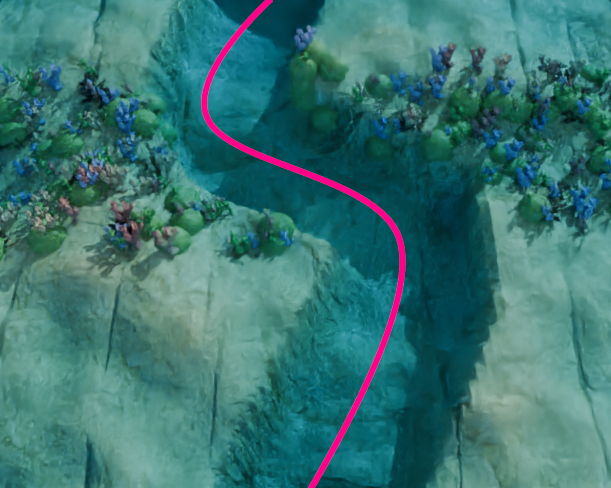
\includegraphics[width = 0.3 \linewidth]{Figures/Interactions/InteractionEdition1.png}
    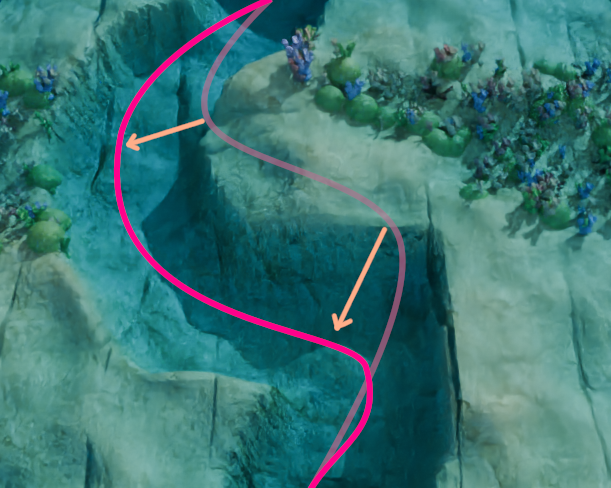
\includegraphics[width = 0.3 \linewidth]{Figures/Interactions/InteractionEdition2.png}
    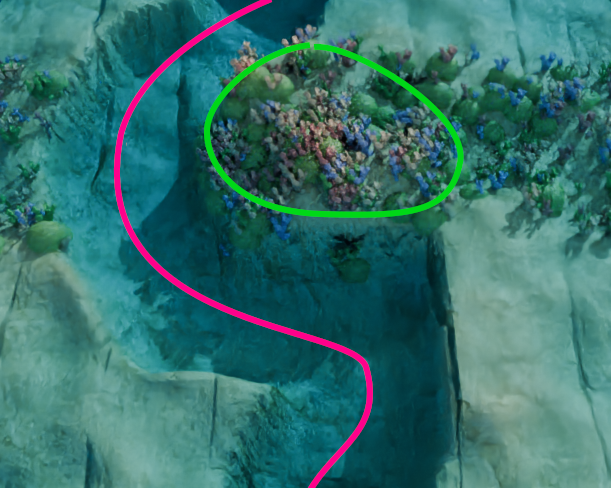
\includegraphics[width = 0.3 \linewidth]{Figures/Interactions/InteractionEdition3.png}
    \caption{Starting from a coral colony developed around a canyon (\textit{left}), the user edits the shape of the canyon, resulting in a different configuration of the scene, killing the corals that ends too deep in the water (\textit{center}) and the development and growth of new corals at the previous location of the canyon (\textit{right}). }
    \label{fig:semantic-representation_user-interaction}
\end{figure}

As long as a non-zero \gloss{FitnessFunc} is defined in the terrain, new \glosses{EnvObj} can be forced by the user at any point of the simulation. 

% \subsection{Guiding the simulation}
Control over the region of the terrain that should be updated can be given by adjusting all \glosses{FitnessFunc} through a scalar field $\influence: \R^2 \to \R $ such that the \gloss{FitnessFunc} $\fitnessFunc(\p)$ of any new \gloss{EnvObj} is evaluated as $\fitnessFunc^*(\p) = \influence{\p} \fitnessFunc(\p)$. This is especially useful in the planning of robotic simulations as we can first generate the overall shape of our terrain and secondly focus the generation process around the areas that may be visited by the robot, avoiding useless simulations and computer power. 
\cref{fig:semantic-representation_coral-colonization-scene} shows an example of colonization of the coral polyps that we limited manually into an annulus.
% \cref{fig:semantic-representation_focus-area-example} shows an example of colonization of the coral polyps that we limited manually.

% \begin{figure}
%     % \centering
%     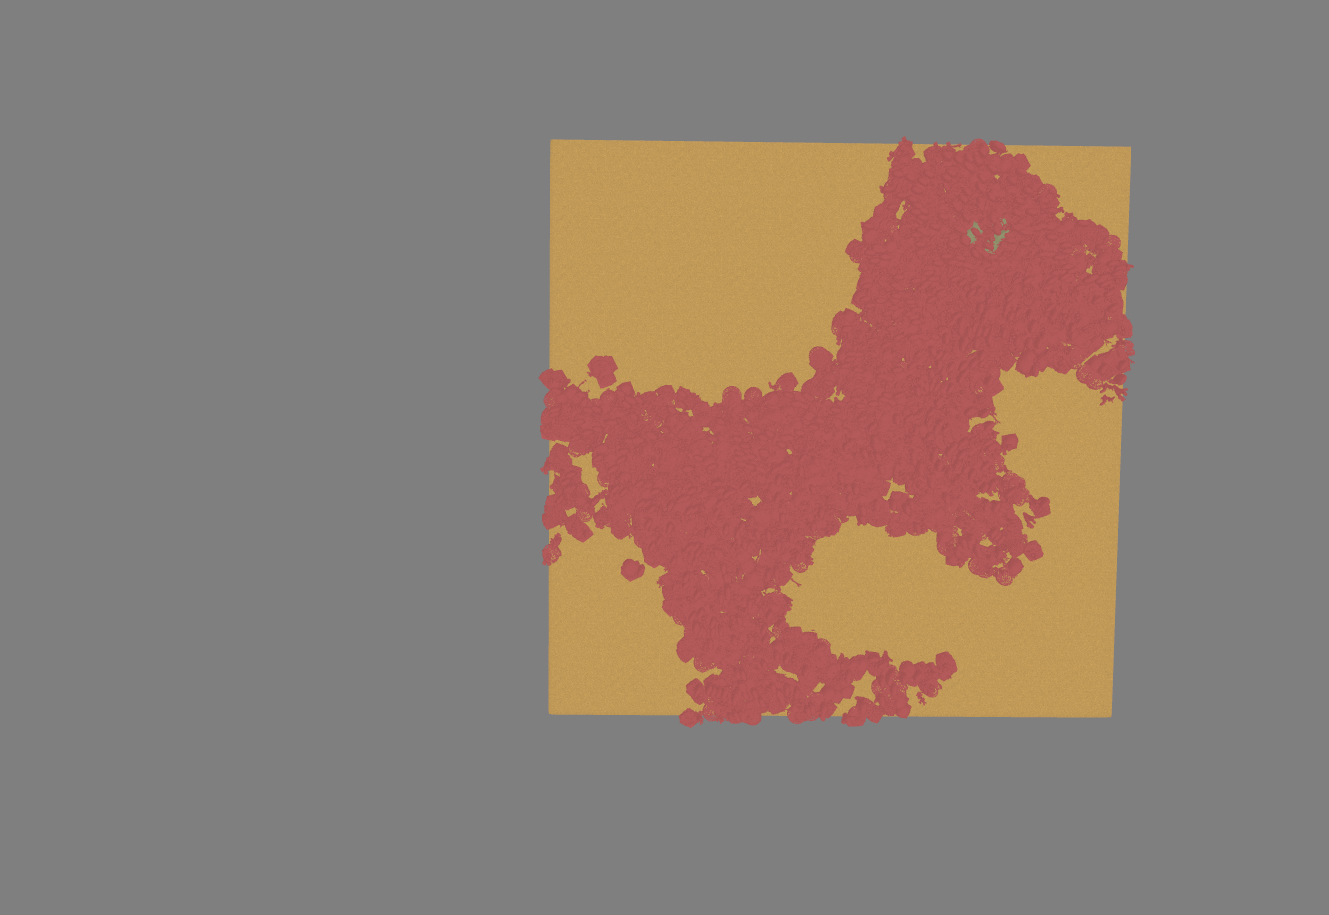
\includegraphics{Figures/UserControl/guidedGeneration1.png}
%     \caption{Controlling the generation area can produce a user-defined focused shape.}
%     \label{fig:semantic-representation_focus-area-example}
% \end{figure}

% - Changing the water currents

Our water current simulation is modeled as a simple vector field. As such, the user is able to interact with it at any moment of the simulation, allowing for the death of sensible \glosses{EnvObj} while it will guide the simulation into a new landscape. By modifying the water currents, the user also modifies the transport rate of \glosses{EnvMat} at this position. The modification of currents is given as a stroke, a parametric curve $\curve$ for which we evaluate $\Delta \Wuser(\p)$ just as for curved environment objects (\cref{sec:semantic-representation_water-currents}).

\subsection{Indirect interaction with \glosses{EnvObj}}
\label{sec:semantic-representation_events}
A configuration file can define in advance the different \glosses{GeoEvent} that should be triggered during the simulation. This can be useful to generate landscapes that are close to some existing locations. 
Multiple \glosses{GeoEvent} can be triggered either as sudden or continuous environmental changes. These changes play a huge role in the morphology of landscapes.
We define \glosses{GeoEvent} with a starting point and an ending point, such that at any time of the simulation we can compute the progress of the \gloss{GeoEvent} as $\tEvent \in [0, 1]$.

Water level changes are important \glosses{GeoEvent} that shape the underwater landscapes. As previously submerged \glosses{EnvObj} get elevated above water level, flora and fauna terrain features dry and die. Deprived from the living part of the features, everything is more affected by terrestrial erosion. By updating the value of the depth $\depth$ evaluated in the \glosses{FitnessFunc}, any \gloss{EnvObj} that is sensible to the depth will be impacted automatically, that may be causing death (\cref{fig:semantic-representation_water-event}). The modification of the water level is defined as 
\begin{align*}
    \depth(\p) = \depth_0(\p) + \sum_{e \in \events} \Delta \depth_e \tEvent
\end{align*}
with $\Delta \depth_e$ the amount of water rising or lowering during an \gloss{GeoEvent}. We assumed a linear evolution of the water level during an \gloss{GeoEvent}. This allows to evaluate the depth at any point in space and in time.

\begin{figure}
    % \centering
    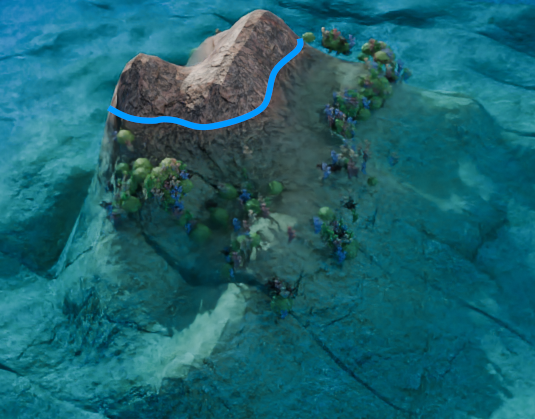
\includegraphics[width = 0.45 \linewidth]{Figures/Interactions/InteractionWater1.png}
    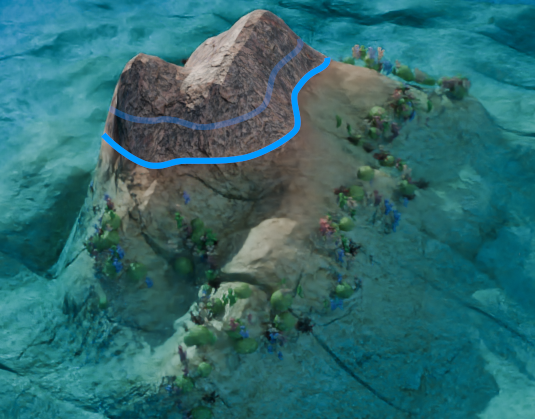
\includegraphics[width = 0.45 \linewidth]{Figures/Interactions/InteractionWater3.png}
    \caption{Lowering the water level by a few meters caused most of the coral objects to satisfy $\fitnessFunc \leq 0$, causing their death. Since the water level (blue) decrease slowly, new coral objects spawn progressively at a lower altitude.}
    \label{fig:semantic-representation_water-event}
\end{figure}

Subsidence and uplift are the main \glosses{GeoEvent} that create or destroy islands in the long term. These \glosses{GeoEvent} are simulated as a simple factor on the height field of the generated terrain (\cref{fig:semantic-representation_subsidence-event}). Subsidence is not always uniform in the terrain. As such, the user can provide a position $\q$ at which the subsidence is the strongest, the amount of subsidence applied $\Delta \height_e$ and a standard deviation $\std$ for which we can then compute at any point in space and time of the simulation the height of the terrain
\begin{align*}
    \height(\p) = \height_0(\p) \cdot \sum_{e \in \events}{G(\norm{\p - \q})} \Delta \height_e \tEvent 
\end{align*}
with $G(x)$ the Gaussian function
\begin{align*}
    G(x) = \exp \left(-\frac {x^{2}}{2 \std ^{2}}\right)
\end{align*}

\begin{figure}
    % \centering
    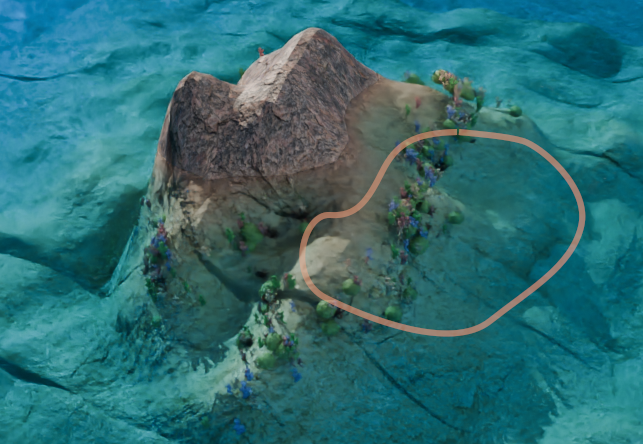
\includegraphics[width = 0.45 \linewidth]{Figures/Interactions/InteractionSubsidence1.png}
    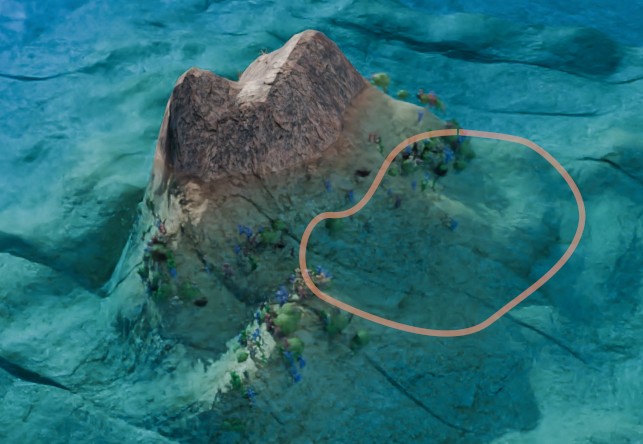
\includegraphics[width = 0.45 \linewidth]{Figures/Interactions/InteractionSubsidence2.png}
    \caption{Simulating subsidence on a part of the terrain (brown area) cause the depth value to change locally, resulting in the death of coral objects that find themselves too deep to survive. Here two subsidence \glosses{GeoEvent} are triggered in parallel. }
    \label{fig:semantic-representation_subsidence-event}
\end{figure}

Storms are factors of the geomorphology of coral reefs \cite{VilaConcejo2016, Oron2023} and coasts \cite{Dominguez2005, Cowart2010}. Due to the extreme wind and wave velocities coasts are highly eroded in a short time period and the more fragile corals near the water surface are broken, possibly causing breaches in the reefs and spreading polyps in the currents direction. While there are many factors at play to understand the apparition of storms and the hydrodynamics affecting it, we simplified the model of storms to the user as a single epicenter $\q$ with a wind velocity $\windVelocity$ and a standard deviation $\std$ representing the spread around the epicenter (\cref{fig:semantic-representation_storm-event}). The computation of water currents are then computed as 
\begin{align*}
    \Wuser(\p) = \Wuser^*(\p) + \sum_{e \in \events} {\windVelocity \frac{G(\norm{\p - \q}}{G(0)}}
\end{align*}
In this case, we did not include the linear factor $\tEvent$ as storms are usually conserving a constant force for the time of the few weeks or months of their occurrence. 

\begin{figure}
    % \centering
    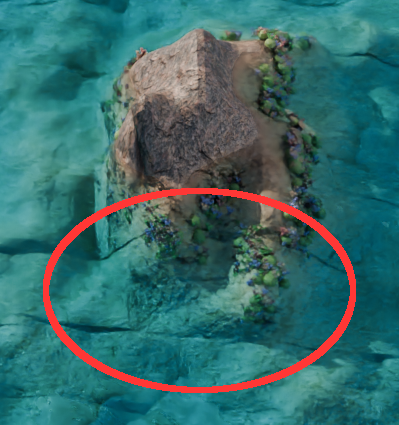
\includegraphics[width = 0.45 \linewidth]{Figures/Interactions/interactionStorm1.png}
    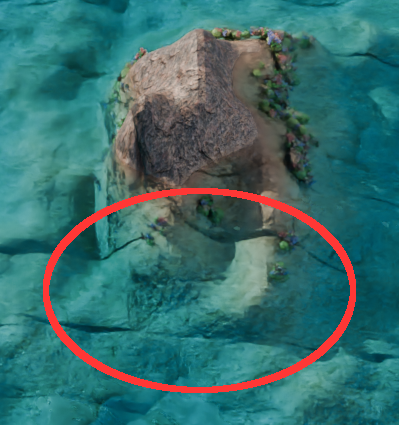
\includegraphics[width = 0.45 \linewidth]{Figures/Interactions/interactionStorm2.png}
    \caption{The result of a storm localized on one side of the island (red area) modifies the result of the evaluation of \glosses{EnvObj} around its epicenter for a short period of time. Most of the coral objects died from the \gloss{GeoEvent}, except few \glosses{EnvObj} less sensible to water currents strength. }
    \label{fig:semantic-representation_storm-event}
\end{figure}

% Just as for the rise and lowering of water level, the heat is modeled as a simple value of the environment. For shallow areas (<100m) we assume a linear relation between depth and temperature, and a constant value for the terrestrial environment. As such, we can model a heat wave by a change of the \glosses{EnvVal}. \Glosses{EnvObj} who are sensible to temperature may die instantly. The modification of the temperature is defined as 
% \begin{align*}
%     \temperature(\p) = T_0(\p) + \sum_{e \in \events} \Delta \temperature_e \tEvent + c \depth(\p)
% \end{align*}
with $\Delta \temperature_e$ the change of heat during an \gloss{GeoEvent}, $\temperature_0$ the temperature at the water surface, and $c$ a very small factor.

The framework can easily be extended as the \gloss{GeoEvent} system stays similar for all \glosses{GeoEvent}. Including higher level simulations in the \gloss{GeoEvent} system can be added, such as the simulation of tectonic activity, the use of fluid dynamics for tsunami \glosses{GeoEvent}, the integration of human activity, ...

\section{Results and discussion}
\label{sec:semantic-representation_results}
Our method provides a way to generate scenes at different scales. We demonstrate this capacity with the generation of a large scene of an island (\cref{fig:semantic-representation_teaser}) after what we focused the generation process in a canyon (\cref{fig:semantic-representation_canyon-scene}), then a small-scale visualization of coral colonies (\cref{fig:semantic-representation_coral-colonization-scene}).
In the examples, we rendered the \glosses{EnvObj} as a implicit tree or as individual meshes. The island, lagoons, reefs, canyons and sand ripples as implicit surfaces

% \subsection{Mid-scale}
% \label{sec:semantic-representation_mid-scale}
A canyon scene can be generated using our method. The water flow is affected by the curve of the canyon such that the currents are oriented in the direction of the curve's tangent.In this example, we force the position of arches to be inside the canyon. The arches deposits a material "rock deposit", which is the main element of the \gloss{FitnessFunc} of the Rock object. The "rock deposit" is slightly affected by water currents, but its mass make it highly affected by gravity. As such, rocks will spawn underneath arches. In reality, an arch is often created as part of a large coral boulder that sees the calcareous bottom part detached by the water currents, often resulting in an arch surrounded by big rocks and smaller rocks from the erosion of the first rocks.
As such, we define an \gloss{EnvObj} "Arch" with a \gloss{FitnessFunc} $\fitnessFunc_{arch}(\p) = 5 - d(canyon - \p) * \norm{\Water(\p)}$, an \gloss{EnvObj} "Rock" using $\fitnessFunc_{rock}(\p) = \material_{rock\_deposit}(\p)$ and Pebble using $\fitnessFunc_{pebble}(\p) = \material_{smaller\_rock\_deposit}(\p)$. Finally, sand ripples are simply described as curves appearing where there is a lot of sand available: $\fitnessFunc_{ripple}(\p) = \material_{sand}(\p)$.
Following these simple rules, \cref{fig:semantic-representation_canyon-scene} shows the emergence of details in the scene. 

% \subsection{Small-scale}
% \label{sec:semantic-representation_small-scale}
In this example we defined three different types of corals, coralA, coralB and coralC, to illustrate the possibility to model behaviours from the choice of \glosses{FitnessFunc}. Each of the coral types deposits a material "coral polyp" and "coral polyp A" ("coral polyp B" and "coral polyp C" respectively). By considering a \gloss{FitnessFunc} that minimize the ratio $\frac{\text{coral polyp}}{\text{coral polyp A}}$, we can see an emergent behavior of the three types of coral fighting for the space colonization.
\cref{fig:semantic-representation_coral-colonization-scene} shows the result of this simulation at three different interations. At the border between two colonies, none of the colonies make progression due to the amount of coral polyp specific from the other colony.

\begin{figure*}
    % \centering
    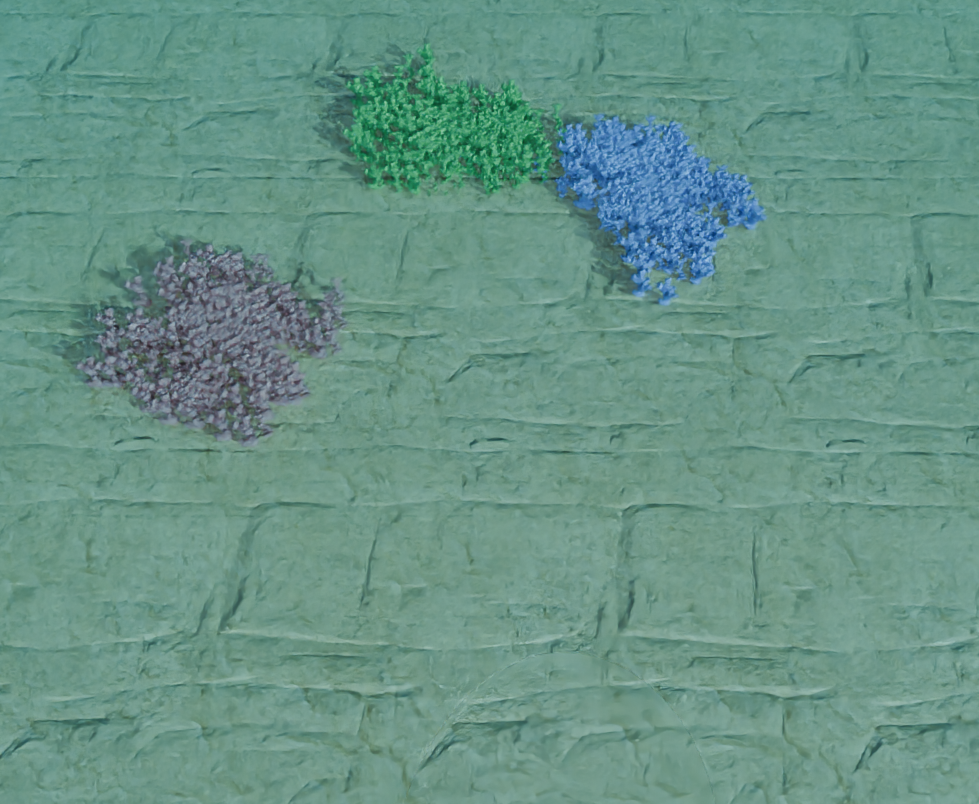
\includegraphics[width=0.24 \linewidth]{Figures/Colonization/col0.png}
    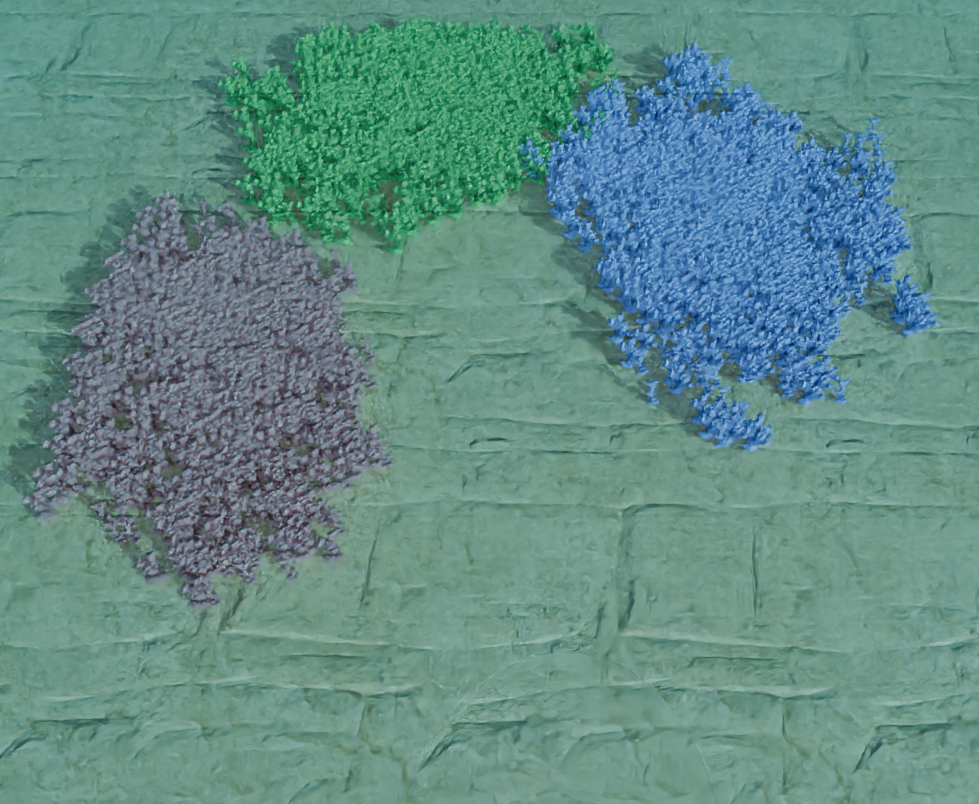
\includegraphics[width=0.24 \linewidth]{Figures/Colonization/col1.png}
    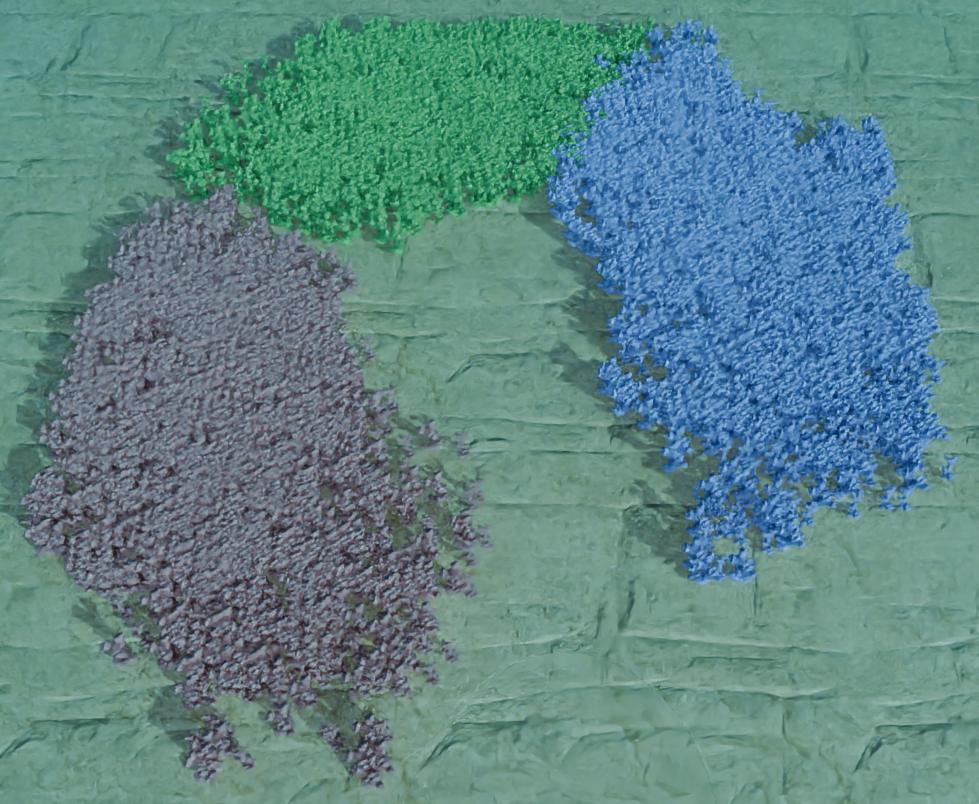
\includegraphics[width=0.24 \linewidth]{Figures/Colonization/col2.png}
    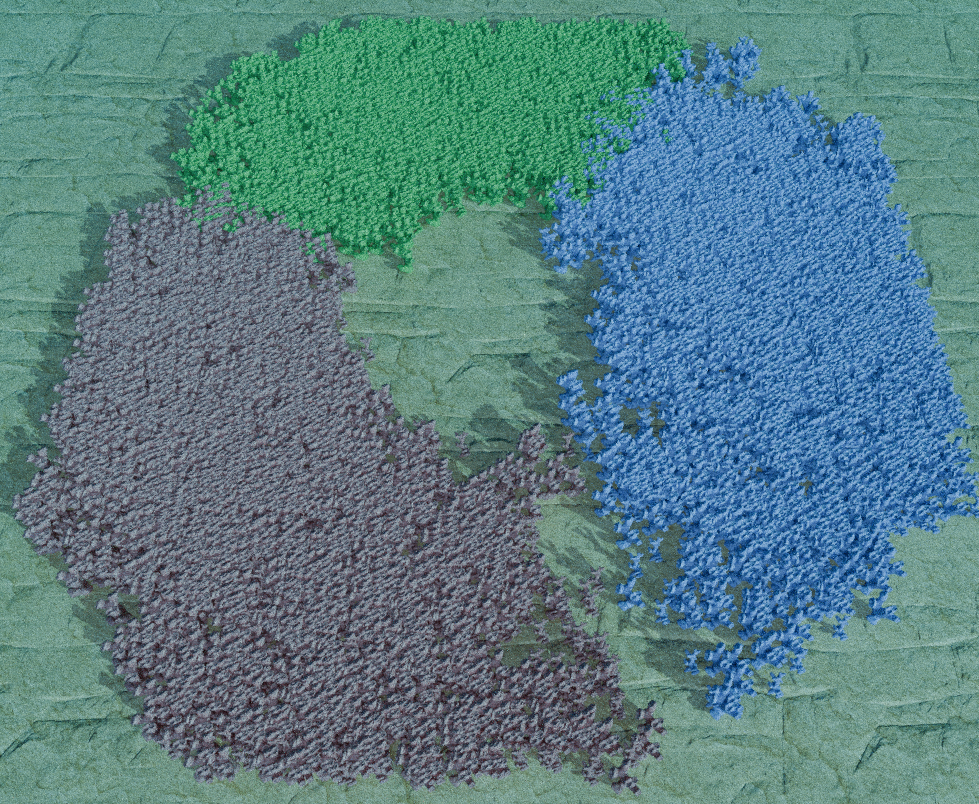
\includegraphics[width=0.24 \linewidth]{Figures/Colonization/col3.png}
    \caption{Three colonies of coral (red, blue, green) restricted to an annulus the middle section of the terrain fighting for the space.}
    \label{fig:semantic-representation_coral-colonization-scene}
\end{figure*}

\begin{figure*}
    % \centering
    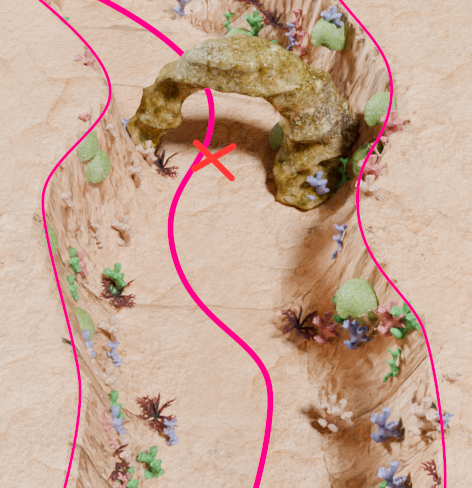
\includegraphics[width = 0.24 \linewidth]{Figures/Canyon/Canyon2.png}
    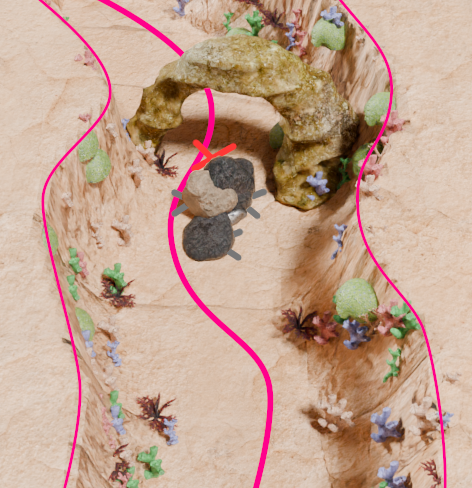
\includegraphics[width = 0.24 \linewidth]{Figures/Canyon/Canyon3.png}
    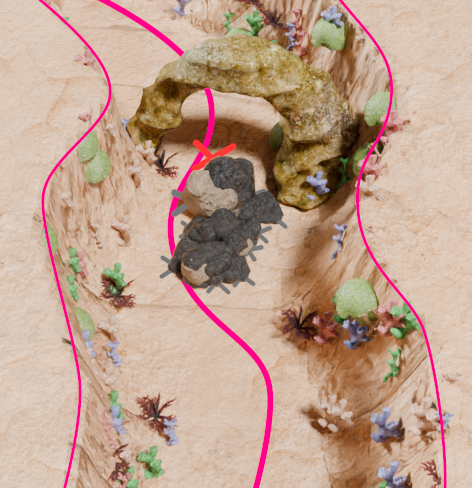
\includegraphics[width = 0.24 \linewidth]{Figures/Canyon/Canyon4.png}
    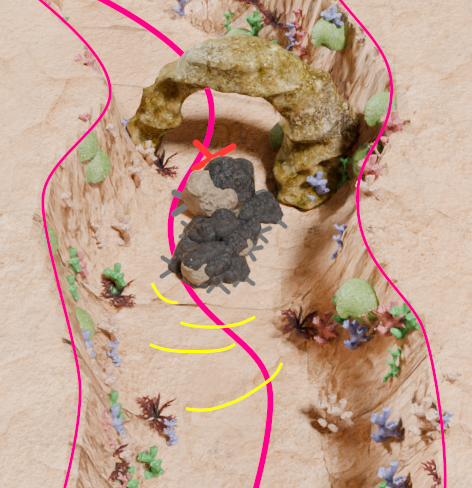
\includegraphics[width = 0.24 \linewidth]{Figures/Canyon/Canyon5.png}
    \caption{Evolution of a canyon scene at different iterations of the simulation. The apparition of an arch causes the spawning of rocks, pebbles, and finally some deposition of sand at the bottom of the canyon, spawning ripples. }
    \label{fig:semantic-representation_canyon-scene}
\end{figure*}


The proposed method aims to generate plausible landscapes using simplified versions of the evolution of an ecosystem and of the 3D representation. The biological realism of the result is highly correlated to the amount of simplification and assumptions, while the visual realism is completely dependent to the geometric functions used for the 3D modeling of the \glosses{EnvObj}. While proposing a flexible method that propose a generic approach for terrain generation, a close collaboration with fields experts and with graphists is needed to achieve optimal results.

Most simulation algorithm's quality depends on the size of the time step used, but with the introduction of a decay rate in the \glosses{EnvMat} properties, we limit the influence of time steps by considering that steady-state are reachable. The material deposition and absorption on punctual \glosses{EnvObj} can be seen as a Dirac function $\dirac$ centered at their position resulting in the advantage that material displacement function can use the definition of the diffusion equation instead of the advection-diffusion-reaction equation. This equation allowing us to evaluate the state of the material $\material$ without intermediate steps, but this is not applicable with curve- and region-based \glosses{EnvObj}. 

\section{Conclusion}
\label{sec:semantic-representation_conclusion}
We have proposed a method to generate terrains procedurally using sparse representations. This representation, the \glosses{EnvObj}, enables to introduce expert knowledge by the mean of the \glosses{FitnessFunc} that rule the \glosses{EnvObj} life cycle, but also to integrate the user in the loop during the generation process. We reduced the terrain resolution limitations by defining the environment objects as parametric features. Thanks to the sparse representation based on single points, curves and regions, we allow for direct manipulation of the \glosses{EnvObj} of the scene by the user which, thanks to the environment steady state consideration, also enables to include these interactions in the automatic simulation process.
Integrating environmental properties in the \gloss{FitnessFunc} of \glosses{EnvObj} allows the user to guide the generation through \glosses{GeoEvent}. Our method enables each \gloss{EnvObj} of the scene to influence the environment locally, reducing the need of computations while also retrieving \glosses{EnvVal} locally, which result in a parallelizable life-like simulation process. The genericity of the environment properties definitions should be sufficient for plausible generation of other landscape types as long as expert knowledge can be translated to \gloss{EnvObj}'s formalism.


We limited our work to the use of 2D scalar fields as they are more easily differentiable, interpretable and lighter than volumetric representations. However, future works include using 3D representations of the terrain and the environment to generate 3D terrains, including cavities, sub-terrestrial areas and the interior of coral structures. 
% The different possibilities to explore for this would be: the use of 3D particles to represent the state of the \glosses{EnvMat} in the environment, or voxel grids or flatten representation of the terrain's surface (but would not allow a different morphological shape than the height field...).

\begin{figure*}
    % \centering
    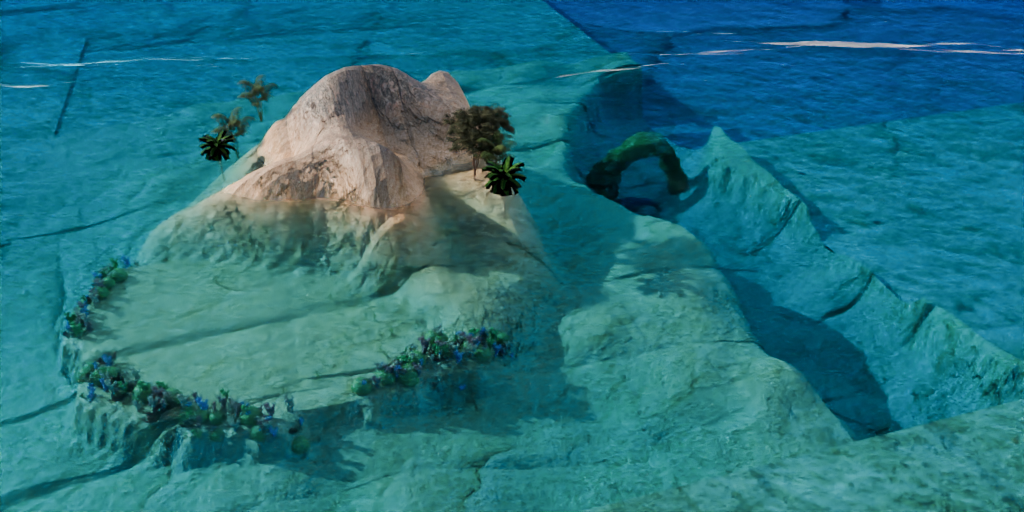
\includegraphics{Figures/CoralIsland/multiScene1 v2 final 1.png}
    \caption{A simple coral reef island is generated using an island, a lagoon, reefs coral polyps, beaches, trees and algae \glosses{EnvObj}. Trees appear on beaches and algae grow in the lagoon's sand. }
    \label{fig:semantic-representation_coral-island-scene}
\end{figure*}














% \section{Method}
% \label{sec:semantic-representation_method}
% The overall pipeline of the method is based on simple incremental generation like most rule-based systems. In this type of system, the final state is defined either by reaching equilibrium, or by verifying specific conditions, such as a maximum number of iterations. 
% We define our pipeline in three phases (\cref{fig:semantic-representation_pipeline}): the initialization phase that describe the generation and simulation rules, the iterative phase generating populating the terrain with our \glosses{EnvObj} and finally the output.


% \subsection{Pipeline overview}





















% \section{Expert knowledge integration}
% \label{sec:semantic-representation_biology}
%   The definition of the \glosses{FitnessFunc} of the \glosses{EnvObj} are inspired by the biological and geological factors that rule the evolution of underwater landscapes. The main factors are depth, light, water currents and biodiversity. External \glosses{GeoEvent} have direct and indirect repercussions on the biodiversity of underwater environments. Coral reef islands are complex bio systems in which fauna, flora and geology are mixed together. 

% \subsection{\Glosses{EnvObj} description}
% \label{sec:semantic-representation_represented-objects}
% We have represented with \glosses{EnvObj} some geologic features, animal features and flora features. The low island is most often raised in a circular shape as the process mainly appear around a hot spot under the ground. The evolution of an island into a coral reef island requires that the environmental conditions are sufficient for coral development: corals will grow slightly below the water surface as waves will break its growth and at a shallow depth (around 3m to 30m deep) in order for light to reach it. As coral grow and die, the skeleton is transformed into porous limestone, providing shelter to surrounding animals and reducing the impact of water erosion on the island. Corals drop polyps that are transported by the water flow and when they stick to a hard surface, as a rock or the reef itself, the coral may grow and colonize the area. As subsidence cause the island to lower, the living part of the coral reef keep growing toward light, which lead to a reef that is constantly close to the water level without reaching it due to wave erosion. The survival of reefs depends on the equilibrium between coral growth and and erosion. Eroded parts of the reef falling in the sheltered part of the reef accumulates, ending up by forming a lagoon. An island formed by a hot spot will inevitably subside in time, until it is completely flatten. As the coral reefs keep growing, only the lagoon remain, resulting in an atoll. \\
% In this work we we integrate the biological and geological knowledge in the \glosses{FitnessFunc} of the \glosses{EnvObj} we want to generate. We represent the islands as regions that can be appearing with a uniform distribution. From the formulation of the region description \eqref{eq:internal-energy-equation}, we mostly create circular islands. The coral features, \glosses{EnvObj} described as a single point, have a \gloss{FitnessFunc} that take into account the depth of the ground, the amount of sand, fresh water and polyps in their environment, as well as the strength of water currents. Each coral species have different living conditions, but we reduced our work to soft coral which are sensible to water strength and stony corals that are more resistant to erosion. Reefs are formed as coral's skeleton are transformed into calcareous stone, describing then as an \gloss{EnvObj} representing multiple others. 

% \subsection{Simplifications}
% \label{sec:semantic-representation_simplifications}
% The environmental factors simulated are greatly simplified as the real processes are in a very small time scale, that computer simulation are not able to simulate in interactive time. The use of \glosses{EnvObj} aim to represent a plausible results, while avoiding modeling the smaller scale \glosses{GeoEvent}. Examples of simplifications are the geometry and material of each \gloss{EnvObj}, which have an influence on the water currents through friction, the water currents represented as stationary flows, while the water flow dynamics are a complex system that may change completely at two different times of the day, the animal influence on the reefs that they transform by the ingestion and deposition of sediments, ...

%
%- What is semantic representation? \\
%** Linguistic definition + Image definition + Our definition \\
%- Why use semantic representation? \\
%** Sharing knowledge with biologists, geologists, etc. \\
%** Data from travel journals, labeled maps, ... \\
%- Advantages and disadvantages of semantic representation \\
%** Advantages: \\
%*** Interpretation \\
%*** User control \\
%*** 3D representation abstraction \\
%** Disadvantages: \\
%*** Need for expert knowledge (+ interdisciplinary communication issues) \\
%*** Necessary simplifications in physics / natural phenomena \\
%- 3D representation of semantic terrains \\
%** Possible combinations of methods (implicit functions + meshes)
%
%\section{Sparse terrain representation}
%- Landscape contains structures of very varying sizes: \\
%** Mountains covering several km² but rivers a few meters wide, for example \\
%- Proposal for sparse terrain representation \\
%** Definition of terrain elements as simple objects: environmental objects \\
%** Implicit geometry, offering 2D or 3D display \\
%** "Easy" LOD possibility \\
%- Iterative method for generating sparse terrain \\
%** Reduce computation time from $O(n^2)$ to $O(n)$ by using the environment as a proxy \\
%** Method based on material deposition \\
%** Iterative stochastic process
%
%\section{Environmental objects}
%- Symbolism of the environmental object \\
%- Reference to "Environmental Objects" \\
%- Comparison to biotopes
%
%\subsubsection{Definition}
%- Skeleton \\
%- Parametric shape \\
%- Living conditions
%
%\subsubsection{Implementation}
%- Instantiation of objects \\
%** Definition of the skeleton \\
%*** Points, curves, regions \\
%*** Use of Snake \\
%** Definition of geometry \\
%- Modifications to the environment \\
%- ...
%
%% \chapter{Snake - Active Contour Model}

We want to symbolize a dead coral area as a \gloss{EnvObj} "reef." To do this, the coral objects continuously deposit a quantity of "dead coral" material. This material, stored in a discrete scalar field, contains high intensities where a reef should supposedly exist. 
We need to draw a curve to represent this new object. The constraints of this curve are that it must pass through the points of highest intensity while maintaining a given length.

The Snake algorithm, or Active Contour Model, approaches this application. The algorithm proposes to give an energy to the curve, which then tries to minimize it through gradient descent.

The energy, in the initial paper, is defined by
\begin{align}
    \Esnake^{*} = \int \limits _{0}^{1} { \Esnake(\mathbf {v} (s))\,ds } = \int \limits _{0}^{1} { \Einternal (\mathbf {v} (s)) + \Eexternal (\mathbf {v} (s)) } \,ds
\end{align}

The internal energy represents the properties of the curve while the external energy represents properties of the field it lies in. In the original paper they are described as: 
\begin{align}
    \Einternal &= \alpha \Econt + \beta \Ecurv \\
    \Eexternal &= \gamma \Eimage
\end{align}

The continuity cost $\Econt$, originally defined as the minimization of the spacing between the points $\left\|{\frac {d{\bar {v}}}{ds}}(s)\right\| ^{2}$, does not make much sense in the discrete form of the algorithm. In its discrete form, we seek to maintain a regular interval between the points by applying $\Econt = \left(\tilde{d} - \left\|p_i - p_{i-1} \right\| \right)^2$ with $\tilde{d}$ being the average distance between each point.

The curvature cost $\Ecurv$ seeks to minimize the oscillations of the curve and can thus be defined as the squared second derivative $\left\|{\frac {d^{2}{\bar {v}}}{ds^{2}}}(s)\right\| ^{2}$.

The discrete form $\Ecurv^{*} = \left\| p_{i-1} - 2 p_i + p_{i+1} \right\| ^2$ is not necessary with splines, due to their closed form.

The image cost $\Eimage$ tries to attract the points of the curve to a local maximum of the image gradient. It is defined as $\Eimage = - \left\| \nabla I \right\| $.

We want to see our curve maintain a given length $L$. We then modify the formulation of the continuity cost to become $\Econt = \left(\tilde{l} - \left\|p_i - p_{p-1} \right\| \right)^2$ with $l = \frac{L}{n - 1}$, knowing $n$ is the number of vertices of the curve. Additionally, we want a curve that follows points of high intensity rather than the gradient, which leads to modifying the image cost $\Eimage = -I$.

The calculation of the gradient $\nabla \Esnake$ remains trivial in parts:
\begin{align}
    \frac{\partial \Eimage}{\partial p_i} &= - \nabla I(p_i) \\
    \frac{\partial \Ecurv^{*}}{\partial p_i} &= -\frac{2 \left( p_{i-1} - 2 p_i + p_{i+1} \right) }{ \left\| p_{i-1} - 2 p_i + p_{i+1} \right\| } \\
    \frac{\partial \Econt^{*}}{\partial p_i} &= 2 \left(l - \left\|p_i - p_{i-1} \right\| \right) \cdot \frac{p_i - p_{i-1}}{ \left\| p_i - p_{i-1} \right\| }
\end{align}

We then have
\begin{align}
    \Esnake &= \alpha \left(l - \left\|p_i - p_{i-1} \right\| \right)^2 + \beta \left\| p_{i-1} - 2 p_i + p_{i+1} \right\| ^2 - \gamma I \\
    \nabla \Esnake &= 2 \alpha \left(l - \left\|p_i - p_{i-1} \right\| \right) \cdot \frac{p_i - p_{i-1}}{ \left\| p_i - p_{i-1} \right\| } - \beta \frac{2 \left( p_{i-1} - 2 p_i + p_{i+1} \right) }{ \left\| p_{i-1} - 2 p_i + p_{i+1} \right\| } - \gamma \nabla I(p_i)
\end{align}

It should be noted that the calculation of $\Econt^{*}$ uses the distance $\left\|p_i - p_{i - 1} \right\|$. For $i = 0$, the distance $\left\| p_i - p_{i + 1} \right\|$ is used.

If all the points of the curve are at a distance greater than $l$, the optimization will push each of these points to get closer to its predecessor. Point $p_0$, itself, will move very little, so the entire curve aligns towards point $p_0$. By using the distance to the successor $\left\| p_i - p_{i+1} \right\|$, the curve moves towards point $p_N$.
It is then possible to converge towards the median point by alternating the use of the distance with the predecessor and with the successor, at the cost of slower convergence.

The active contour model algorithm is highly sensitive to the initial curve placement. In cases where a portion of the curve is in an area with a very low gradient on $\Eimage$, the vertices of the curve will simply optimize $\Einternal$, resulting in a straight segment in a low-intensity area, while the rest of the curve optimizes correctly.

To mitigate this problem, we propose adapting the Snake algorithm into Caterpillar: throughout the gradient descent, the target length $L$ is artificially reduced and then increased. In this way, a portion of the curve blocked in a region without possible optimization on external energy will be attracted by the optimized curve until it falls on a strong gradient. The dead portion can take the place of optimized vertices. By returning the target length $L$ to its initial value, the optimization continues with fewer vertices in the dead zone. Repeating this process gradually brings all points into an optimizable area. However, a too-rapid change in the target length can prevent the vertices from optimizing $\Eexternal$ by amplifying $\Einternal$ too much. Additionally, this algorithm can lead to numerical errors and slower convergence.

%
%\subsection{Communication between objects}
%- Comparisons with reality \\
%** No direct communication between elements \\
%- ...
%
%\subsubsection{Interactions through the environment}
%- Modifications to the environment \\
%** Absorption \\
%** Deposition \\
%** Modification of currents \\
%- Impact of the environment on objects \\
%- ...
%
%\subsubsection{Lifecycle of environmental objects}
%- ...
%
%\section{Results}
%- ...


%\subsection{Implemented tools}
%- Cost function parser \\
%- ...

%\section{Other attempts}
%\subsection{Direct interactions}
%\subsubsection{Graph generation}
%\subsubsection{Delaunay triangulation}


%
%\section{Continuous erosion}
%[POSSIBLY TO BE MOVED TO EROSION] \\
%- ...
%
%\subsection{Problem description}
%- Erosion process is a dynamic system \\
%- Very large number of variables \\
%- Impossible to simulate at different time steps and/or different scales/resolutions
%
%\subsection{Proposed solutions}
%- ...
%
%\subsubsection{Lifecycle of environmental objects}
%- ...
%
%\subsubsection{Use of deep learning}
%- ...




%\chapter{Influence sur la génération}
\label{chap:influence-on-env-objects}
\minitoc


\section{Introduction}
\label{sec:influence-on-env-objects_introduction}
This document aims to formalize a terrain generation method developed during my thesis.

The main issue this method seeks to address is the difficulty for a user to describe the environments they want to generate. By proposing a hierarchical structure in the description of elements to define, the environments exhibit adaptive representation granularity, catering both to the user's needs and hardware capabilities.

The key element of the method is the "biotope," defined as "a habitat defined by relatively uniform physical and chemical characteristics." (Source: Wikipedia)

In this context, we define the characteristics of a geographical region as well as the sub-biomes included within it.

Although this method was conceived with the aim of generating underwater environments, many examples given in this document will use elements present in surface environments, purely for simplification purposes.

\section{Glossary}
\label{sec:influence-on-env-objects_glossary}
Initially, this document will present definitions of various terms used in the description of the method. By doing so, we hope to eliminate any ambiguity in the upcoming explanations. Definitions may appear in certain sections of this document if deemed too specific.

\textbf{Biotope}: The main element of the method used. The biotope (or, as I might often write, the biome) is a geographical region defined by topographic and geomorphological characteristics. The notion of biotope used does not distinguish between different scales (the biosphere and the ecosystem of a rock are represented uniformly), nor does it distinguish between living and mineral elements. The biotope is represented in two different ways in the terrain generation process: the model and the instance.

\textbf{Model (of biotope)}: The model (or biotope model, if the context requires) is a biological description of the geographical area. It remains an abstract, or literary, form of the biotope. It is defined by a list of characteristics related to topography (description of the relief, description of the shape of the region) and geology (type of soil, for example). One can also list the sub-biomes that compose it, specifying the quantity, proportion, chances of appearance, etc., of each sub-biome. This form is the user input into the system, but during the terrain generation process, the model's role is to create instances of itself to concretize the structure to be generated. In the document illustrations, if a model is represented in a graph, it will be symbolized by its name in quotation marks (e.g., "Forest," "Lagoon").

\textbf{Instance (of biotope)}: The instance is the concrete form of the model. Unlike the model, the instance takes place in space with fixed characteristics (unlike the probabilistic characteristics of the model). Through generation rules and living conditions defined by the user and the system, the biotope instance has a geometric shape and neighboring relationships with other instances. An instance, like its original model, consists of sub-biomes. The instance remains linked to its original model. To distinguish the instance from the model in the document illustrations, if represented in a graph, the instance will be symbolized by the model's name followed by a hash and an instance number (e.g., Forest \#1, Lagoon \#28).

\textbf{Generation Rule}: Generation rules represent a list of obligations or prohibitions, including living conditions and adjacency rules.

\textbf{Living Condition}: In our definition, a biotope can only exist under certain environmental conditions in a specific place. The conditions can be multiple and will be listed in a subsequent chapter of this document. Vegetative elements, for example, have strong constraints in terms of sunlight exposure, the "snow" biotope requires a low temperature condition, and some biotopes like sand cannot exist on steep terrain. Living conditions are therefore important properties to express in biotope models. These conditions can be expressed probabilistically.

\textbf{Adjacency Rules}: Adjacency rules define how biotope instances can be arranged. There are three types of rules to express adjacency between two biotopes: prohibition, possibility, and obligation. Two models linked by an adjacency prohibition cannot generate instances with a common border. Conversely, a model linked to another by an obligation constraint can only generate an instance if it shares a border with an instance of the linked model. The possibility constraint is the default, where the instance is indifferent to the presence or absence of a common border. It is conceivable that the notion of "possibility" could be associated with a probability in the future, allowing for example, a lake to often be adjacent to an urban area, but an urban area to rarely be near a desert. For now, adjacency rules are bilateral: a rule that applies from biotope A to biotope B also applies from B to A. In the rest of the document, adjacency rules will mainly be represented by graphs (undirected) with the nodes as the models to be generated, solid edges representing the possibility of adjacency, dotted edges symbolizing an adjacency obligation (rarely used), and the lack of an edge indicating an adjacency prohibition.

\textbf{Adjacency Graph}: The adjacency graph, although similar to the representation of adjacency rules, this time represents the concrete topological adjacency between the generated instances (not the models). The adjacency graph consists of nodes representing each instance generated by the models and the edges representing the existence of a common border. Edges can only be present if the two biotope instances see their model linked either by an obligation or possibility of adjacency constraint. By definition, this graph must be planar. In this document, adjacency graphs will therefore be represented by graphs where the nodes are biotope instances (following the instance graphic convention), and an edge represents a topological adjacency.

\textbf{Region (of biotope)}: The region is the space occupied in a geometric sense by a biotope instance once represented in space. Among the important properties, one can note that a region has a shape and an area.

\textbf{Boundaries}: The boundary is the geometric adjacency of two regions representing biotope instances.

\textbf{Adjacent Regions}: Two regions are adjacent if they share a common edge. In a successful generation, a region shares a common boundary with regions represented by instances linked to the current region instance in the adjacency graph. We can then distinguish three types of connections between instances: correctly adjacent instances are linked in the adjacency graph and are adjacent regions, over-adjacent instances are not linked in the adjacency graph and are adjacent regions, and under-adjacent instances are linked in the adjacency graph and are not adjacent regions. The latter two types are maladjacencies.

\textbf{Biotope Characteristics}: Biotopes possess characteristics common at all scales, whether they represent geological or biological elements. The characteristics are defined in the models in probabilistic forms. Instances inherit a unique and fixed value for each characteristic from the original model. The characteristics notably define the shape the generated region will take, the relief, etc.

\textbf{Sub-biotope}: Each biotope can include one or more sub-biomes. This is how an environment can be defined on the scale of a planet as well as on the scale of a rock. The biotope specifies the number of instances to generate for each sub-biome, or the proportion of the surface to cover. The parent biotope provides an approximate description of its environment, but with each sub-biome, the description is refined.

\textbf{Recursive Tree}: The proposed method has a strong recursive nature through its representation in biotopes and sub-biomes. The biotope construction tree is thus a recursive tree of biotopes composed at the root of a biotope to be generated and whose nodes (and leaves) represent sub-biomes. The parent-child relationship defines the inclusion of the child among the sub-biomes of the parent node. The tree describing a biotope can then be reused to describe a larger biotope, up to a planetary scale or larger.

\textbf{User Action}: The user plays an important role in the terrain generation process. By user action, we mean any action performed during the process. User actions are applied to biotope instances: adding, replacing, or deleting an instance, or modifying the characteristics and living conditions of an instance.

\textbf{Primitives}: Primitives are simple geometric representations that can be combined to represent more complex structures. Among these, we can notably find: the point, the curve, the sphere, and the 3D model.

\section{Environment description}
\label{sec:influence-on-env-objects_environment-description}
In this method, an environment is defined by a biotope model for which characteristics such as the general shape of its region, the biotope's relief, or the representative primitive of the biotope are specified, as well as living conditions such as altitude, temperature, and necessary luminosity for its survival. These characteristics are uniform across the entire biotope region; the only way to vary them is to add sub-biomes in the definition, which will take the form of sub-regions of the parent. Sub-biomes have the same types of characteristics and living conditions, which they can define in their own way, as well as their own sub-biomes.

Thus, the environment description is carried out recursively until the level of detail is sufficient for the modeler.

A biotope model can be the sub-biome of several different biotope models, offering the possibility to define complex environments quickly.

\subsection{Biotope characteristics}
The biotope model allows the user to describe the biotope's appearance to be generated. This description is probabilistic, and instances derived from the model each define a unique value for each characteristic respecting the probability law described by the model. The list of characteristics includes:
\begin{itemize}
	\item Region size: This represents the area of the surface (without considering relief) that the region occupies in space.
	\item Altitude (min and max): These two characteristics represent the altitudes the biotope can reach.
	\item Relief (frequency and amplitude): These characteristics describe the terrain's gradient. High relief amplitude symbolizes significant disturbances on the ground, unlike low amplitude, which
	
	indicates the ground is relatively flat.
	\item Primitive (type, dimension, position): The primitive determines the basic element represented by the biotope.
	\item Shape: The biotope region's shape in space.
\end{itemize}

To facilitate the user's work, default values are proposed for each biotope, respecting each type of primitive.

\subsection{Living conditions}
The living conditions of a biotope define the specific properties necessary for the biotope to survive. To be viable, the biotope must respect these conditions. These properties may relate to the following conditions:
\begin{itemize}
	\item Luminosity (min and max)
	\item Temperature (min and max)
	\item Soil type
	\item Exposure (direction, minimum and maximum angle)
\end{itemize}

Like characteristics, default living conditions are proposed to the user.

\subsection{Adjacency rules}
Three types of rules express adjacency between two biotopes: prohibition, possibility, and obligation. These rules define how biotope instances can be arranged spatially.

\begin{itemize}
	\item Prohibition: Two models linked by an adjacency prohibition cannot generate instances with a common border.
	\item Possibility: Instances can be adjacent, but it is not required.
	\item Obligation: Instances must share a common border.
\end{itemize}

\section{Generation process}
\label{sec:influence-on-env-objects_generation-process}
The terrain generation process involves creating instances from biotope models while respecting their characteristics, living conditions, and adjacency rules. This section details the steps of the process.

\subsection{Instance creation}
Each biotope model creates instances with fixed values for each characteristic derived from the probabilistic descriptions in the model. These instances are then positioned in space according to their characteristics and living conditions.

\subsection{Placement and adjustment}
Instances are placed in the environment, respecting their adjacency rules. If instances violate adjacency constraints, adjustments are made to either reposition instances or modify their characteristics within acceptable limits.

\subsection{User interaction}
Users can intervene in the generation process by adding, replacing, or deleting instances, as well as modifying instance characteristics and living conditions. These actions allow for fine-tuning the generated environment.

\subsection{Validation and refinement}
The final step involves validating the generated environment by checking for over- or under-adjacencies and making necessary refinements to ensure all instances adhere to their constraints and living conditions.

\section{Conclusion}
\label{sec:influence-on-env-objects_conclusion}
This method provides a structured approach to terrain generation by leveraging biotopes and their hierarchical organization. By defining biotopes probabilistically and respecting adjacency rules and living conditions, it is possible to generate diverse and realistic environments with varying levels of detail.

Future work may include refining probabilistic models for characteristics and adjacency rules, as well as exploring the use of probabilistic adjacency possibilities to further enhance the flexibility and realism of generated terrains.
%- ...
%
%\section{Biotope generation}
%- ...
%
%\subsection{Definition}
%- ...
%
%\subsubsection{Recursion}
%- ...
%
%\subsubsection{Voronoi diagram}
%- ...
%
%\subsubsection{Communication between biotopes}
%- ...


\part{Modelisation}

\chapter*{Abstract}
\label{chap:modelisation-abstract}
- Methods completely different \\
** Physical phenomena are different \\
** => Simulation/generation methods must be specific for one landscape \\
- Methods are developed at different instants of the thesis work, \\
** We will see different procedural generation domains: \\
*** Analytical solutions (coral islands \#1) \\
*** Deep Neural Networks (coral islands \#2) \\
*** 3D user interaction (karst networks) \\
- Deep Learning tends to replace procedural methods in 2D domain, \\
** But still too complex for 3D models \\
*** (lack of data, lack of research interest for now) \\
** Still requires a lot of data, which, is (while not easy) possible using aerial images, but is way too sparse with underwater landscapes or underground biomes. \\
- We want to control the area in which an element is modeled in the terrain \\
** Because that's how we define them in the previous chapter. \\
** Thus we cannot use simple random noise methods => no bounds \\
*** Only solution is to use falloff maps, but meh... \\
- As such, we want to keep the skeleton of our elements using primitives (points, curves, regions) \\
** => Much easier to add constraints / manipulate primitives in a "procedural generation" way. \\
- Warning: usage of Deep Learning is at the limit of "procedural generation" and is not considered as part of it by the whole community. \\
(Complete with the Reddit poll). \\
- ... 


\chapter{Graphical representation of environmental objects}
\label{chap:representation-env-objects}
- Implicit surfaces \\
- Meshes \\
- ...


% \chapter{Volumetric Terrain Modeling [MAYBE TO BE MOVED TO INTRO]}
\label{chap:volumic-modeling}
\minitoc

- Volumetric modeling is important for representing 3D structures \\
- Allows for the representation of cavities, arches, overlays, etc. \\
- The concept of materials allows for including much more information for the following parts: amplification and rendering \\
** Amplification (e.g., erosion) needs to know the type of soil at the surface and subsurface to be realistic \\
** Rendering needs to know the material at the surface to correctly display textures \\
- ...

\section{Implicit terrains with materials}
\label{sec:volumic-modeling_implicit-terrain-with-materials}
- ...

\subsection{Material density}
- ...

\subsubsection{Material granularity}
- ...

\subsubsection{Soil triangle}
- ...

\subsection{Scalar functions}
- ...

\subsection{Blending functions}
- ...

\subsection{Placement functions}
- ...

\subsection{Material usage}
- ...

\subsubsection{Defining the final material}
- ...

\subsubsection{Post-processing: material transformation}
- ...

\section{Graphical Representation of \glosses{EnvObj}}
\label{sec:volumic-modeling_graphic-representation-env-objects}
- Implicit surfaces \\
- Meshes \\
- ...


\graphicspath{ {./figures/cGAN_figures/} }

\chapter{Automatic generation of coral reef islands}
\label{chap:coral-island}
\teaser{
	\centering
	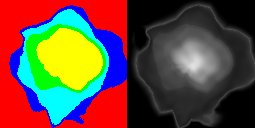
\includegraphics[width=0.6\linewidth]{terrainGAN.png}
	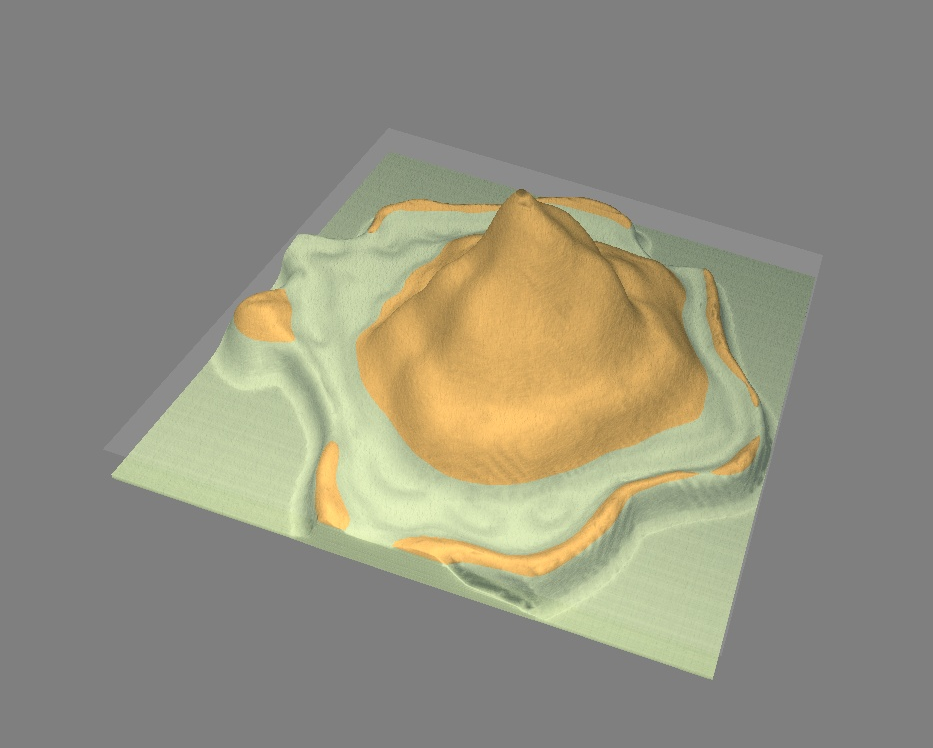
\includegraphics[width=0.3\linewidth]{terrainGAN_result.png}
	\caption{Caption.}
	\label{fig:teaser_cGAN}
}

\abstract 
In this chapter, we propose a procedural method for generating single circular volcanic islands using user sketching from two perspectives: a top view, which defines the island's shape (horizontal dimensions), and a profile view, which outlines its elevation and terrain (vertical dimensions). These perspectives, commonly used in geological and remote sensing domains, are complemented by a user-defined wind field, applied as a distortion field to deform the island's shape, mimicking the effects of wind and waves. Based on these inputs, our method generates a height field of the island. This algorithm is capable of creating many different island models, and we have generated thousands of exemplars to compose the dataset used for training a conditional Generative Adversarial Network (cGAN). By applying data augmentation, the cGAN allows for even greater variety in the generated islands, providing users with more control over the shape and structure of the final output.
\pagebreak 

\minitoc

\section{Introduction}
\label{sec:coral-island_introduction}

Coral reef islands are formed through a dynamic interplay of volcanic activity, coral growth, and long-term geological processes. These islands begin as volcanic landmasses, created when magma from the Earth's mantle erupts through the ocean floor and builds up layers of volcanic rock, eventually rising above sea level. In tropical waters, these volcanic islands create ideal conditions for coral reefs to develop. Corals, thriving in the shallow, sunlit waters around the island, initially form fringing reefs attached to the island's coastline.

As time passes, the volcanic island undergoes subsidence, a slow sinking process caused by the cooling and contraction of the Earth's crust beneath the island. In response to this subsidence, corals continue to grow upward, maintaining their position within the photic zone, where sunlight supports their survival. This upward growth leads to the formation of barrier reefs, which become separated from the island by a lagoon as the island sinks further.

Eventually, the volcanic island may submerge completely beneath the ocean's surface, leaving only the coral structure visible above water. This process results in the formation of atolls, which are ring-shaped reefs encircling a central lagoon. Over geological time, the physical structure of the island evolves from a prominent volcanic peak to a coral-dominated reef system, shaped by the combined forces of subsidence, coral growth, and erosion.

% 
Charles Darwin's subsidence theory, developed from his observations during the voyage of the HMS Beagle, remains one of the most widely accepted explanations for the formation of coral reef islands. Darwin proposed that coral reefs form around volcanic islands that slowly subside over time due to geological processes. As the volcanic island sinks, coral reefs grow upward, maintaining their position near the surface of the ocean. This theory explains the transition from fringing reefs attached to the island's coast, to barrier reefs separated by a lagoon, and finally to atolls, where the volcanic island has completely submerged, leaving only the coral structure visible above water.

While other theories, such as John Murray's growth on submerged mountains and Reginald Daly's sea level change theory, have also been proposed to explain coral reef formation, Darwin's subsidence theory remains the most widely supported due to its ability to account for the full evolution of coral islands, from volcanic landmasses to atolls. Its simplicity and focus on the relationship between subsidence and coral growth make it especially well-suited for computational modeling.

In our approach, we translate the core principles of Darwin's theory into a procedural generation model, simulating the gradual sinking of volcanic islands while coral reefs grow to keep pace with changing sea levels. This allows us to realistically model the transformation of islands from volcanic landmasses to coral-dominated atolls. By capturing this interplay, we can procedurally generate a wide variety of island structures that reflect real-world geological processes.

%

Simulating the formation of coral reef islands presents significant challenges due to the complex interplay of geological, environmental, and biological factors. One major difficulty lies in capturing the long-term subsidence of volcanic islands, which occurs over millions of years, while simultaneously modeling the upward growth of coral reefs that rely on environmental conditions such as water depth, temperature, and sunlight. This combination of slow geological processes and dynamic biological growth is difficult to replicate in a computational model.

Additionally, the biological aspects of coral growth are inherently tied to environmental factors. Coral reefs grow only within a specific range of water depth and sunlight, and their growth patterns are affected by the health of the reef ecosystem and the availability of resources. Accurately modeling these biological dependencies in a procedural system is challenging, as the factors governing coral reef development are difficult to generalize.

Existing terrain generation methods, such as Perlin noise-based algorithms or uplift-erosion models, are often ill-suited for these processes. While they can generate natural-looking landscapes, they do not account for the unique geological and biological interactions that govern coral island formation. Capturing these dynamics requires a balance between realism and procedural flexibility, allowing for both accurate simulation of natural processes and intuitive user control.

%

To address these challenges, we present a procedural generation tool that simulates the formation and evolution of coral reef islands by integrating both geological and biological processes. Our approach allows users to control the island's shape and structure through intuitive sketching interfaces, while the tool handles the complex dynamics of subsidence, coral growth, and environmental deformation.

The generation process begins with two user-defined inputs: a top view to outline the island's overall shape and a profile view to define its elevation and terrain contours. These inputs serve as the foundation for creating a height field of the island. Additionally, a wind deformation field allows the user to simulate the effects of wind and waves, reshaping the island's structure in a way that mimics natural erosion processes.

To enhance flexibility and allow for more complex, non-circular island structures, we incorporate a conditional Generative Adversarial Network (cGAN) into the generation process. The cGAN is trained on a dataset of islands generated by the initial algorithm, augmented to introduce a wider variety of shapes and features. This machine learning component allows for the automatic generation of diverse island models, removing some of the constraints of the initial procedural algorithm such as strictly radial symmetry while maintaining user control over key aspects of the design.

By combining user input with the adaptive power of the cGAN, our tool generates realistic coral islands that evolve from volcanic landmasses to coral-dominated atolls, capturing both geological and environmental processes.



\section{Overview}
Our system for generating coral reef islands combines user-driven sketching, procedural techniques, and deep learning to create realistic and varied island terrains. The process begins with the user sketching key features of the island, such as its overall shape and profile. This sketching process allows the user to define the layout of the island in an intuitive way, providing control over the placement of important elements like the island borders, beaches, lagoons, and coral reefs.

Once the user's sketch is complete, the system converts these high-level features into a labeled map, where each pixel is assigned to a specific region of the island. This map serves as the input to a conditional Generative Adversarial Network (cGAN), which is responsible for generating the fine details of the terrain. The cGAN has been trained on a dataset of island examples generated by the initial procedural algorithm, allowing it to produce realistic terrains that reflect the user's design while introducing natural variation and complexity.

By conditioning the cGAN on the user-defined map, the system maintains the overall structure and regions specified in the sketch, while generating realistic transitions between different areas (such as beaches, lagoons, and the island's interior). The use of deep learning, in combination with procedural techniques, allows the system to create coral islands that are both geologically plausible and tailored to the user's input.

This method provides a flexible yet powerful approach to island generation, enabling the creation of diverse island structures that reflect real-world geological processes, such as volcanic subsidence and coral reef growth.



\section{Related works}
Procedural generation of terrain has been a well-researched area in computer graphics and simulations, where the goal is to create large, realistic landscapes with minimal manual input. Various methods have been developed over the years to generate terrains automatically, from noise-based approaches to physically-based erosion simulations, sketch-driven methods, and more recently, deep learning techniques.

However, each of these techniques has its strengths and limitations, particularly when it comes to modeling coral reef islands. Coral islands present unique challenges due to the combination of long-term geological processes (such as subsidence and coral reef growth) and environmental interactions (like erosion caused by wind and waves). In this section, we review the key techniques that have been applied to terrain generation, highlight their limitations for coral island formation, and position our work as an approach that addresses these challenges.

\subsection{Noise functions}
% Noise functions
Noise-based procedural generation remains one of the most widely used techniques for creating natural-looking terrains. Introduced by Ken Perlin, the Perlin noise and Simplex noise are foundational algorithms that generates pseudo-random yet continuous variations across a grid, producing terrain features that resemble organic landscapes \cite{Perlin1985,Perlin2001}.

Beyond basic noise functions, more advanced techniques, such as Fractal Brownian Motion (FBM), are commonly used to add additional detail to terrains. FBM combines multiple layers, or "octaves," of noise at different frequencies, creating terrains with finer details and more realistic features. Noise functions are often paired with falloff maps to generate island-like terrains, where the height of the terrain gradually decreases toward the edges, mimicking the appearance of coastlines and providing a simple way to create basic island shapes.

Despite their widespread use, noise-based methods have significant limitations when applied to the simulation of coral reef islands. While these techniques excel at producing large, varied landscapes quickly, they lack the geological accuracy needed to model real-world processes like volcanic subsidence and coral growth. These approaches generate random patterns, but are disconnected from the actual physical processes that govern coral island formation.

Our approach goes beyond the randomness of noise-based generation by incorporating real-world geological and biological processes into terrain formation. Specifically, we model the gradual subsidence of volcanic islands and the upward growth of coral reefs, which are essential for representing the long-term evolution of coral reef islands. By integrating these processes into the generation algorithm, we create terrains that are not only more realistic but also allow for user control. This blend of user input and geological grounding provides a more accurate and flexible approach to modeling coral reef islands, addressing the limitations inherent in traditional noise-based techniques.

\subsection{Erosion simulation}
% Erosion simulation
While noise functions generate random, natural-looking terrain, they often fail to capture the physical processes that shape real landscapes over time. To address this limitation, erosion simulations model how natural forces such as water flow and gravity wear down terrain features, creating valleys, river networks, and other detailed landforms. These simulations are particularly effective at representing mountainous landscapes, where erosion gradually sculpts the terrain over long periods of time, typically on the scale of thousands to millions of years.

Erosion simulations often use models like the Stream Power Law to describe how water erodes higher elevations and deposits sediment in lower areas. The rate of erosion depends on factors such as slope steepness and water flow, with steeper slopes and greater water volumes leading to faster erosion. Over time, these processes create detailed and realistic terrain features like river valleys and erosion channels. Erosion models are iterative, simulating the gradual shaping of landscapes by continuously balancing forces like erosion and uplift, as seen in the work of \cite{Cordonnier2016,Cordonnier2017a}. Their model simulates how tectonic forces uplift terrain, which is then eroded away over thousands of years. Similarly, \cite{Schott2023} and \cite{Tzathas2024} refined the Stream Power Law to generate realistic slopes and ridges through these long-term geological processes.

Despite their effectiveness in modeling large-scale terrain evolution, erosion simulations are limited when it comes to representing environments that are shaped by dynamic biological processes. Coral reefs, for instance, grow and adapt to changing environmental conditions on a much shorter timescale than geological erosion. While erosion models simulate terrain changes over millennia, coral growth responds more dynamically to factors like water depth, light availability, and temperature on scales ranging from years to decades. These biological factors are difficult to incorporate into traditional erosion models, which are designed to simulate the slow, steady forces of water and gravity.

Our approach builds on the concept of terrain evolution by integrating the geological and biological dynamics that shape coral reef islands. Instead of focusing solely on erosion, which is primarily a surface-level process, we model the subsidence of volcanic islands over geological time and the simultaneous growth of coral reefs that adapt to the changing sea levels. Coral reefs must grow upward to remain within the photic zone, a process that unfolds on shorter timescales than those captured by standard erosion simulations. Furthermore, we introduce wind deformation to simulate the effects of environmental forces like wind and waves, which dynamically reshape the island's structure over time. This combination of long-term geological processes and short-term biological responses provides a more comprehensive simulation of coral reef island formation, capturing both the slow subsidence of volcanic landmasses and the rapid adaptability of coral ecosystems.

\subsection{Sketching}
% Sketching

In procedural terrain generation, sketch-based approaches allow users to directly interact with and shape landscapes through intuitive sketching interfaces. These methods enable users to define key terrain features such as mountains, valleys, and coastlines by drawing them in a two-dimensional canvas, which are then translated into 2.5D terrains. Sketching provides a high level of artistic control, making it especially popular in creative applications such as video games and simulations, where user-defined terrain features are prioritized.

Sketch-based systems offer great flexibility, allowing users to directly define specific elements of the landscape according to their needs or preferences. For instance, \citep{Gain2009} introduced a multi-perspective sketching system that allows users to generate detailed landscapes by sketching from different angles. This method provides more control over the terrain's shape than traditional noise-based generation methods. Similarly, \citep{Tasse2014} explored sketching from the player's viewpoint, allowing users to dynamically define height information from within the virtual environment, creating an interactive terrain design experience.

Sketching has also been extended to geological modeling. \citep{Patel2021} proposed a system where users can interactively model underground layers by sketching subsurface structures. This provides a powerful tool for geologists and designers who need to model complex, multi-layered terrains, offering more control over both the surface and the subsurface.

In our work, we leverage the flexibility of sketching to define the key features of coral reef islands, such as the island shape, lagoons, and coral reefs, in a vectorized format. This is particularly important for modeling underwater and island landscapes, where these features are not simply surface elements but part of an evolving geological structure. By using sketches, we retain the semantic information of where the island and coral regions are located, which allows us to later apply our simplified model of Darwin's subsidence theory.

Rather than focusing on detailed long-term or short-term evolution, our method adapts sketching to the unique requirements of island and underwater landscapes. Once the user defines the terrain layout through sketching, we apply a simplified subsidence model, where the volcanic island gradually sinks and coral reefs grow in response, remaining close to the water surface. This process provides a framework for simulating the evolution of the landscape in a geologically plausible manner.

The key advantage of sketching in our system is that it combines the artistic control provided by traditional sketching methods with the ability to handle the geological processes specific to coral reef islands. By preserving the vectorized information from the sketch, we can accurately place and evolve features like lagoons and coral reefs, ensuring that the resulting terrain reflects both the user's design intent and the geological dynamics at play.

\subsection{Deep learning}
% cGAN

In recent years, deep learning has become a transformative tool in computer graphics, image processing, and procedural content generation. Deep learning refers to a class of machine learning techniques that use artificial neural networks with multiple layers to model complex patterns in data. By training these networks on large datasets, deep learning models can learn to generate new, realistic data by identifying the underlying relationships between inputs and outputs.

In terrain generation, deep learning is particularly well-suited to tasks that require the creation of complex, natural-looking landscapes. Traditional procedural generation techniques like noise functions and erosion simulations can be powerful, but they often struggle to produce the complexity and realism of natural terrains due to their reliance on predefined rules and algorithms. In contrast, deep learning models, especially Generative Adversarial Networks (GANs), can learn from data, enabling them to generate realistic terrains that mimic the diversity and complexity found in nature.

GANs are a particularly effective deep learning architecture for terrain generation. A GAN consists of two neural networks: a generator, which creates new data samples, and a discriminator, which evaluates whether the generated samples are real or fake compared to a set of training data. Through this adversarial process, the generator gradually improves its ability to produce realistic examples, while the discriminator becomes better at distinguishing real from fake data. This feedback loop allows GANs to generate highly realistic and detailed terrain features by learning from large datasets of existing terrains.

In terrain generation, GANs have been applied to generate diverse landscapes by learning the patterns and features found in real-world terrains. For example, \citep{Guerin2017} demonstrated how GANs can be used to transform 2D sketches into 3D terrains by training the network on a dataset of terrain features, allowing the system to generate new landscapes based on simple user input. GANs are particularly well-suited for this task because they can capture the subtle details of terrain that would be difficult to model explicitly, such as the natural flow of elevation or the transitions between different terrain types.

A variant of GANs, known as Conditional Generative Adversarial Networks (cGANs), takes the power of GANs one step further by allowing the generated data to be conditioned on additional inputs. In a cGAN, both the generator and the discriminator receive additional information such as a class label, a sketch, or an image, that guides the generation process. This makes cGANs particularly useful for terrain generation tasks where users want to control specific aspects of the output while still relying on the model to generate realistic details.

In the case of terrain generation, a cGAN allows the user to specify high-level constraints (such as the outline of an island or the regions where different terrain types should be) while the generator fills in the finer details based on what it has learned from the training data. This makes cGANs particularly effective in applications where a mix of user input and data-driven generation is required, as the user can control the broad layout of the terrain while the model ensures that the resulting terrain looks natural and plausible.

In our approach, we use a cGAN to generate coral reef islands, providing a balance between user control and realistic terrain generation. After the initial algorithm outlines the regions of the island such as the island itself, beaches, and lagoons, these regions are transformed into a single image, where each pixel represents a different region ID. This image is used as the input for the cGAN, which conditions the generation process on this initial layout.

The cGAN is trained on a dataset of island examples, which are created by the initial procedural generation algorithm and further augmented to introduce a wide variety of shapes and features. This training allows the cGAN to generate coral reef islands that follow the high-level layout provided by the user while introducing natural variations and details that reflect real-world island characteristics. By conditioning the cGAN on the user-defined region map, we ensure that the generated islands maintain structural coherence while still exhibiting realistic features like smooth transitions between regions, varied terrain, and non-circular shapes.

One of the key advantages of using a cGAN in our system is its ability to overcome procedural constraints. Traditional procedural generation methods often impose limitations like radial symmetry or require islands to follow overly simplified geometries. With the cGAN, these constraints are lifted. The model can generate irregular, non-circular islands that adhere to the user's input but introduce a level of complexity and realism that would be difficult to achieve with purely procedural methods.

Additionally, the cGAN ensures that the generated island terrain aligns with the geological processes modeled in the system, such as subsidence and coral reef growth. By training the cGAN on thousands of examples that reflect these processes, we ensure that the final generated island models are both flexible and geologically plausible. The combination of user-driven design and data-driven generation through the cGAN allows for the creation of coral reef islands that are not only tailored to the user's input but also realistic in their form and structure.



\section{Example generation}
\label{sec:coral-island_example-generation}

Generating synthetic coral reef island terrains involves a combination of user input, procedural techniques, and simplified geological simulations. The process begins with the creation of a base terrain using user-defined sketches, followed by a simulation of coral reef growth and subsidence. These two steps, although interconnected, can also be used independently, providing flexibility in how the system is applied. In this section, we describe the example generation process in detail.

\subsection{Assumptions}
In generating synthetic coral reef islands, we adopt a set of simplifying assumptions that are grounded in geological and biological observations. These assumptions streamline the process while producing plausible terrains. Below, we outline the key characteristics of our model:

% \begin{itemize}
    \textit{Radial symmetry:} Volcanic islands often begin as circular landmasses due to the radial uplift of magma from beneath the Earth's mantle. Erosion processes further smooth out sharp edges over time, reinforcing this initial symmetry. In our approach, we assume islands start with an approximately circular shape, providing a straightforward basis for terrain generation.
% This assumption reflects real-world volcanic islands, such as those in the Pacific, where erosion gradually shapes the initial circular form. Starting with a radial structure simplifies the generation and serves as a solid foundation for further deformation.

    \textit{Coral growth at constant depth:} Coral reefs require sunlight to thrive, which limits their growth to depths where light penetrates the water. In our model, coral growth is constrained to this depth range, with corals maintaining their proximity to the water surface as the volcanic island subsides.
% Coral growth follows biological principles, growing upward in shallow waters. This assumption simplifies the process of modeling coral features and reflects the observed behavior of real coral reefs.

    \textit{Radial arrangement of features:} The key island features like the island body, beaches, lagoons, and coral reefs, are arranged in concentric regions around the island center. This radial arrangement aligns with natural geological progression from the island to the surrounding reef.
% This simplifies the generation process by organizing features in a predictable order, similar to coral atolls where lagoons and reefs form protective rings around the island.

    \textit{Wind and wave deformation:} Over time, wind and wave forces shape islands by introducing concave regions, carving out lagoons, and deforming coastlines. To simulate these effects, we apply a wind deformation field that allows users to introduce natural variations that break the radial symmetry, resulting in more realistic island shapes.
% Wind and wave erosion play a significant role in shaping real coral islands, and simulating this erosion adds natural-looking variation. The wind field gives the user control over how much deformation is applied, creating non-uniform, dynamic island coastlines.

    \textit{Independence of islands:} In this model, each island is treated as an independent entity, meaning its terrain does not influence neighboring islands. This allows multiple islands to be generated and placed freely without concern for terrain overlap or interaction. 
% This assumption reflects the typical formation of islands in archipelagos, where individual islands are geographically separate. It simplifies the generation of multi-island scenes by avoiding unnecessary inter-island interactions.

    \textit{Uniform profile shape:} We assume that the vertical profile of the island remains relatively uniform, meaning that the terrain's cross-section from the center outward is similar in every direction. This allows for consistent scaling of the profile in all directions, ensuring that the island's shape remains coherent and plausible.
% Although real-world islands can have local variations in their profile, this uniformity makes the generation process more manageable and produces consistent terrain features.

    \textit{Subsidence and coral growth:} As the volcanic island subsides, coral reefs grow to keep pace with the sinking landmass, maintaining their height near the water surface. In our model, the island subsides as a whole, while coral features are preserved by growing vertically. This separation allows the coral regions to remain unaffected by the subsidence of the island itself.
% This assumption is based on Darwin's subsidence theory, which explains the formation of coral atolls. Modeling coral growth independently of the island's subsidence ensures the coral regions stay at the water surface as the island sinks.
% \end{itemize}

These assumptions, while simplified, provide an effective foundation for generating coral reef islands. They balance computational efficiency with geological plausibility, ensuring that the generated terrains are both flexible and realistic. Furthermore, the system allows users to break the radial symmetry and introduce more natural variations through wind deformation, adding another layer of flexibility to the model.


\subsection{User Input}

The generation of coral reef islands in this system begins with two intuitive sketch-based inputs from the user: a top-view sketch and a profile-view sketch, which define the islands horizontal layout and vertical elevation profile. In addition to these sketches, the user can further refine the terrain by applying wind deformation strokes, which simulate the effects of wind and waves on the islands shape. This combination of sketches and wind inputs gives users precise control over both the islands structure and its natural variations, such as irregular coastlines or concave features.

\subsubsection{Top-view Sketch}

The top-view sketch defines the islands outline as seen from above. Using a simple drawing interface, the user can delineate the boundaries between key regions of the island, including the island itself, the beaches, the lagoon, and the surrounding abyss. The system assumes that these regions are arranged concentrically around the center of the island, with each boundary defined by a radial distance from the center.

Each region's boundary is represented in polar coordinates, with $\radius_\p$ indicating the radial distance from the islands center and $\theta_\p$ representing the angular position. This polar representation allows the system to map the users sketch onto a circular framework, ensuring smooth transitions between regions and maintaining a coherent layout for the island.

In this sketch, the user defines the overall horizontal layout of the island, including the size and shape of each feature. Variations in the outline can be introduced by allowing the radial distances to vary with angle, ensuring that the island is not strictly symmetrical and introducing more natural, irregular shapes.

\subsubsection{Profile-view sketch}

The profile-view sketch defines the vertical elevation profile of the island along any radial direction, offering control over the islands height. In this view, the user specifies the elevation of different regions of the island, such as the island peak, beach, lagoon, and abyss, by marking a set of milestones along the profile.

These milestones correspond to key terrain transitions: the highest point of the island (center), the island border, the beach, the lagoon, and the deep-sea abyss. The system uses these milestones to interpolate a continuous 1D height function $\heightProfile(x)$, where $x \in [0,1]$ represents the normalized radial distance from the islands center, and $h = \heightProfile(x)$ gives the height at each point. This continuous profile ensures smooth elevation transitions across the island.

By combining the top-view and profile-view sketches, the system can generate a full 3D terrain model that accurately reflects the users design.

\subsubsection{Wind velocity field}
In addition to the sketches, the user can influence the shape of the island by defining a wind velocity field. This field simulates the effects of wind and wave erosion on the island's surface, introducing natural deformations such as coastline indentations, concave features, or variable lagoon shapes.

The wind field is represented as a series of wind strokes drawn by the user on a 2D canvas. Each stroke represents a parametric curve, where the direction and strength of the wind are encoded as a vector field. The user controls the wind's direction by drawing these curves, and the system interprets the strokes to create a velocity field that defines how the terrain should be deformed.

As the user draws a wind stroke, the system generates a set of control points along the curve, with the option to adjust the stroke's width. The width of each stroke determines the area of influence around the curve, where wider strokes result in broader deformations of the terrain.
The deformation strength decreases with distance from the wind curve using a Gaussian falloff function using the stroke width as standard deviation, ensuring that the terrain transitions smoothly from deformed regions to non-deformed areas.
Once the wind strokes are applied, the system processes the wind velocity field by displacing the terrain points accordingly. The height field, originally generated from the user's sketches, is modified by the wind field to create non-radial features, breaking the initial radial symmetry and producing a more organic island shape.

\subsubsection{User interaction}

As users draw the top-view and profile-view sketches, the system provides real-time feedback on the resulting terrain. The top-view sketch influences the horizontal layout of the island, while the profile-view sketch defines its vertical structure. These sketches can be adjusted independently, allowing the user to fine-tune both the outline and elevation of the island.

After sketching the basic shape, users can apply wind deformation strokes to modify the island's features further. These strokes represent wind and wave influences, distorting the island's shape to introduce more natural, non-radial features such as indentations along the coastline, variable lagoon shapes, or concave formations. The system automatically applies these deformations, providing real-time feedback as the user interacts with the terrain.

This interactive process, combining sketches and wind deformation, allows users to quickly iterate on their designs, refining the terrain to meet specific aesthetic or functional goals.




\subsection{Generation process}
The generation of coral reef island terrains involves a structured process that takes the user's sketches and produces a complete 3D terrain model. This process begins with the creation of the initial height field based on the user's input, followed by the application of wind deformation to introduce natural variations, and concludes with the integration of coral reef features through subsidence and coral growth modeling.

\subsubsection{Initial height field generation}
The generation of the coral reef island terrain begins by transforming the user-defined top-view and profile-view sketches into a coherent 3D height field. This process combines the radial layout of the top-view sketch with the elevation information provided by the profile-view sketch, creating a terrain that accurately represents the desired features, such as the island, beaches, lagoons, and abyss.

For any point $\p$ on the terrain, the system first computes the polar coordinates $(\radius_\p, \theta_p)$, where $\radius_\p$ is the radial distance from the island's center, and $\theta_p$ is the angular component. The radial distance $\radius_\p$ is used to determine which region the point belongs to (island border, beach, lagoon, or abyss). The user-defined milestones in the profile sketch specify the radial boundaries between these regions.

Each point's height is determined by the profile function $\heightProfile(x)$, where $x$ represents the normalized radial distance from the island's center. The function $\heightProfile(x)$ is continuous and defines the height of the terrain at any point along the profile, from the island's center (at $x = 0$) to the outer boundary of the abyss (at $x = 1$).

The system first identifies which region the point $\p$ falls into by comparing $\radius_\p$ with the radial boundaries defined by the milestones. These milestones divide the terrain into sections, such as:
\begin{itemize}
    \item Island: $\radius_\p \leq \radius_{\text{island}}$,
    \item Beach: $\radius_{\text{island}} < \radius_\p \leq \radius_{\text{beach}}$,
    \item Lagoon: $\radius_{\text{beach}} < \radius_\p \leq \radius_{\text{lagoon}}$,
    \item Abyss: $\radius_{\text{lagoon}} < \radius_\p \leq \radius_{\text{max}}$
\end{itemize}

For any point between two milestones (e.g., between the island border and the beach), the system computes the normalized distance $x_\p$ using linear interpolation between the radial distances of the two milestones. For example, if $\radius_\p$ is between the beach boundary $\radius_{\text{beach}}$ and the lagoon boundary $\radius_{\text{lagoon}}$, the value of $x_\p$ is computed as:

\begin{align}
    x_\p = \frac{\radius_\p - \radius_{\text{beach}}}{\radius_{\text{lagoon}} - \radius_{\text{beach}}}
\end{align}

This normalized distance $x_\p$ represents the position of point $\p$ relative to the region's boundaries.

Once the correct value of $x_\p$ is determined, the height of the point $h(\p)$ is computed directly using the profile function $\heightProfile(x)$, which smoothly defines the height for any given value of $x$. The height function $\heightProfile(x)$ is continuous across all regions, ensuring that transitions between the island, beach, lagoon, and abyss are smooth.

For any point $\p$, the height is computed as:
\begin{align}
    h(\p) = \heightProfile(x_\p)
\end{align}

This approach ensures that the height field accurately follows the elevation profile specified by the user while maintaining smooth transitions between different regions of the island.

By using the profile function $\heightProfile(x)$ to directly compute the height for any point on the terrain, the system guarantees smooth transitions between regions (e.g., from the island to the beach or from the lagoon to the abyss). This method eliminates the need for separate interpolation between regions, as the function $\heightProfile(x)$ is defined continuously across all regions of the island.

The result is a height field that captures both the radial structure of the island (from the top-view sketch) and the vertical elevation profile (from the profile-view sketch), producing a realistic representation of coral reef islands with smooth transitions between the key terrain features.



\subsection{Wind deformation}

After generating the initial height field based on the top-view and profile-view sketches, the next step in the process introduces wind deformation. This step simulates the long-term effects of wind and wave erosion, breaking the radial symmetry of the terrain and adding natural variations such as concave coastlines and irregular island shapes.

% \subsubsection{User-defined wind field}

The wind deformation can be controlled through a user-defined vector field, which represents the direction and strength of wind flows across the terrain. Users interact with the system by drawing strokes on a 2D canvas, which are then interpreted as parametric curves $\curve$ representing wind patterns. Each stroke defines a wind flow in the curve's direction $\curve'$ and an effect width $\std$, and these wind flows are used to displace the terrain, simulating the gradual reshaping of the island due to wind and wave erosion.

The strokes are represented as Catmull-Rom splines, a type of parametric curve that allows for smooth, continuous wind paths. For any point $\p$ on the terrain, the deformation vector $\warp(\p)$ is calculated based on the proximity of $\p$ to the nearest wind strokes. The strength of the displacement is controlled by a Gaussian scaling function, which ensures that points closer to the wind strokes experience stronger displacement, while points farther away are less affected.

The displacement $\warp(\p)$ is computed as a sum of the influences from all nearby wind strokes. For each stroke, the deformation vector is scaled by a Gaussian function that decreases with the distance from the closest point $\q$ on the parametric curve $\curve$, as follows:

\begin{align}
    \warp(\p) = \sum_{\curve \in \text{curves}} \curve'(\q) \cdot e^{-\frac{\norm{\p - \q}^2}{2 \std^2}}
\end{align}


% \subsubsection{Deformation process}
Once the deformation vector $\warp(\p)$ is computed, the terrain height at point $\p$ is adjusted by displacing $\p$ to a new point $\warp(\p)$.
We can then compute the final height $h(\warp \circ \p) = \heightProfile(t_{\p})$, or, as the implicit modeling community would write it, 
\begin{align}
    \Tilde{h}(\p) = \warp^{-1} \circ h
\end{align}

This process introduces variations in the terrain, distorting the coastline, creating concave regions, and breaking the original radial symmetry defined by the top-view and profile-view sketches.

\subsubsection{Resistance to deformation}

To ensure that certain regions of the terrain, such as deep-water areas, remain relatively unaffected by the wind, a resistance function $\rho(x)$ is applied. The resistance function modulates the effect of the wind deformation based on the radial distance $\radius_\p$ from the island's center, which is normalized to a value $x \in [0, 1]$.

The resistance function $\rho(x)$ is defined similarly to the profile function, and it controls the magnitude of the displacement at each point. For example, regions near the coastline (such as the beach and lagoon) might have lower resistance, allowing for more significant deformation, while regions farther away (such as the abyss) have higher resistance, limiting the wind's impact.

The deformation vector is scaled by the resistance function at each point $\p$, such that the final deformation vector becomes:

\begin{align}
    \Tilde{\warp}(\p) = \rho(x_\p) \cdot \warp(\p)
\end{align}

Where $\rho(x_\p)$ is the resistance value corresponding to the point's normalized distance $x_\p$. This ensures that the wind deformation has the greatest impact on areas like the coastline and beach, where erosion naturally plays a larger role, while deeper regions like the abyss remain stable and relatively unchanged.

\subsubsection{Deformation and height field update}

The wind deformation process results in a modified height field where the terrain has been warped according to the user-defined wind strokes. This deformation introduces non-radial features, such as concave coastlines or irregularities along the beach and lagoon, making the island appear more natural and varied.

Both the height field and the labeled map (which tracks the terrain regions like island, beach, and lagoon) are updated to reflect the wind deformation. This ensures that the semantic information of the terrain remains consistent even after the terrain has been warped. The labeled map is deformed in the same way as the height field, preserving the logical structure of the island for further post-processing, such as texturing.

For instance, consider a simple circular island generated from the initial height field. By applying wind strokes along one side of the island, the deformation process can create concave regions along the coastline, making the shape more irregular and mimicking the effects of real-world wind and wave erosion. The resistance function ensures that while the beach and lagoon areas are deformed, the abyss remains largely unaffected as they are far from the wind and wave effective areas, preserving the island's overall structure.




\subsection{Coral reef modeling}

Once the terrain has been generated and deformed by the wind, the system simulates the subsidence of the volcanic island and the growth of coral reefs. These processes reflect the long-term geological evolution of coral reef islands, where the volcanic island gradually sinks (subsides) while coral reefs grow upward to keep pace with the sinking landmass.

\subsubsection{Subsidence}

The subsidence of the island is modeled by scaling the initial height field downward, simulating the effect of the volcanic island slowly sinking into the ocean. The user provides a subsidence rate $\lambda$, which represents the proportion by which the island has sunk over time. The subsidence is applied uniformly to the terrain, meaning all points on the island sink by the same factor.

The subsided height field $h_{\text{subsided}}(\p)$ is computed by scaling the original height field $h_0(\p)$ with the subsidence factor $\lambda$:

\begin{align}
h_{\text{subsided}}(\p) = (1 - \lambda) \cdot h_0(\p)
\end{align}

Where:
- $\lambda \in [0, 1]$ is the subsidence rate (e.g., $\lambda = 0.2$ means the island has subsided by 20% of its original height),
- $h_0(\p)$ is the height at point $\p$ from the initial height field.

This scaling reduces the overall height of the island, simulating how volcanic islands sink over time due to tectonic activity and erosion. The subsidence factor $\lambda$ is applied uniformly across the terrain, meaning that all points on the island experience the same degree of subsidence, regardless of their original height or location.

\subsubsection{Coral reef growth}

As the volcanic island subsides, coral reefs grow upward to remain close to the water surface, following the “keep-up” strategy observed in real-world coral formations. Coral growth is restricted to regions where the depth is within the optimal range for coral development, typically from the water surface to around 30 meters below.

The coral reef features (reef crest, back reef, and fore reef) are modeled separately from the subsidence process. The system generates a coral feature height field $h_{\text{coral}}(\p)$, which remains unaffected by the island's subsidence. This height field ensures that coral regions remain near the water surface, even as the island sinks.

Coral reef growth is entirely independent of the subsided terrain. Even as the volcanic island sinks, coral growth is driven only by the proximity of terrain to the water surface, ensuring that coral features always remain near the surface, irrespective of how much the island subsides.

The coral reef height field is generated using predefined depth values for the various coral regions:
- The reef crest is modeled near the water surface, typically just below sea level,
- The back reef and lagoon are slightly deeper but remain within the range where corals can grow,
- The fore reef slopes downward into the deep ocean, transitioning into the abyss.

The system uses these predefined regions to assign heights to coral reef points based on their proximity to the reef crest. For example, the height of a point in the fore reef is interpolated between the reef crest height and the deeper abyss regions.

\subsubsection{Blending the height fields}

The final step is to blend the subsided height field $h_{\text{subsided}}(\p)$ with the coral feature height field $h_{\text{coral}}(\p)$ to produce the final terrain. The goal is to ensure that coral features remain near the water surface while allowing the rest of the island to subside.

To achieve this, the system uses a smooth max function, which smoothly blends the two height fields. The smooth max function ensures that the coral regions dominate where coral growth is present, while the subsided island terrain dominates in other regions. This blending method ensures that the transition between the coral and subsided regions is smooth and visually consistent.

The smooth max function adapted from Ingo Quilez's smooth min function is defined as:

\begin{align}
    \smoothmax(a, b, k) = a + \frac{(b - a)}{1 + \exp\left(-k \cdot (b - a)\right)}
\end{align}

Here, $a = \heightSubsid(\p)$ is the height from the subsided island, $b = \heightCoral(\p)$ is the height from the coral reef feature, and $k$ controls the smoothness of the transition.

This smooth max function guarantees visual continuity by preventing abrupt height differences between the coral regions and the subsided terrain, creating a smooth, gradual transition that mimics the natural blending of coral reefs with deeper areas. The coral feature height field takes precedence where coral can grow, typically in shallow regions up to around 30 meters below the water surface. In deeper regions, such as the abyss, the subsided height field naturally dominates, ensuring that the final terrain accurately reflects both subsidence and coral growth processes.

\subsubsection{Output}

The resulting terrain represents a realistic coral reef island, where the volcanic island has subsided, and coral reefs have grown upward to keep pace with the water level. The smooth blending between the subsided terrain and the coral features ensures a natural transition between regions like the island, lagoon, and coral reefs.

One of the key strengths of this method is its flexibility: 
- The subsidence and coral reef growth processes are modeled independently, allowing for a wide range of configurations. Users can generate plausible island terrains with or without coral features, or apply the coral reef growth simulation to existing height fields from other sources.
- Additionally, the coral reef growth simulation can be fine-tuned by adjusting the predefined depth values for different coral regions, allowing for further customization of the terrain's appearance.





\section{Conditional Generative Adversarial Networks}

In this section, we introduce the use of a Conditional Generative Adversarial Network (cGAN), specifically the pix2pix model, to enhance the island generation process by increasing the variety and flexibility of terrains. While the initial procedural algorithm can create numerous island examples, cGAN provides additional flexibility in generating more complex terrain without the rigid constraints of the first algorithm.

\subsection{Introduction to cGAN}

A Generative Adversarial Network (GAN) consists of two competing neural networks: a generator that attempts to produce realistic data, and a discriminator that tries to distinguish between real and generated data. In the conditional GAN (cGAN) variant, both the generator and discriminator are conditioned on some input, meaning the generated output is influenced by additional information, such as a labeled map or image.

For island generation, we use the pix2pix model, a specific cGAN designed for image-to-image translation. In this case, the input to the generator is a labeled map which is a 2D image where each pixel is assigned an ID representing a different region of the island (e.g., island body, beach, lagoon, coral reef). The output is an image where each pixel corresponds to the elevation of the terrain at that point, ie. a height field.

\subsection{cGAN for island generation}

The cGAN model was chosen for this task because it allows us to overcome some of the constraints of the initial procedural algorithm. While the first algorithm generates island terrains based on radial symmetry and a limited set of input parameters, cGAN can generate more complex and varied terrains by learning from a large dataset of examples. Specifically, the use of cGAN addresses the following challenges:

1. Increased Variety: The cGAN model can generate a wide range of island shapes and terrains by learning from the dataset. This allows for the creation of terrains that go beyond the predefined structures of the initial algorithm, introducing more natural variation in island features.

2. Overcoming Constraints: In the initial algorithm, islands are always centered in the image and adhere to a radial symmetry. Using cGAN, we apply data augmentation (translation, scaling, and combining multiple islands in one sample) to remove these constraints, allowing islands to take more irregular shapes and positions.

3. Flexibility: Once trained, the cGAN model acts as a black box that generates island terrains based on the labeled input. While this limits user control during the generation process, the model can produce a variety of terrains that still respect the underlying structure of the labeled map. This enables a flexible, rapid generation process without requiring the user to fine-tune parameters manually.

\subsection{Training}

The cGAN model is trained using a dataset of island terrains generated by the initial algorithm. To create this dataset, the algorithm randomly generates top-view shapes for the island's features, adds noise (such as fractional Brownian motion, or fBm), and introduces random wind velocity fields. The profile function remains consistent in determining the relative positions of the island, beach, and lagoon, but the top-view shapes vary through noise and deformation.

\subsubsection{Data augmentation}

To enhance the variety of the dataset and improve the model's ability to generalize, we apply several data augmentation techniques:
- Translation: Since the original algorithm always centers the island, we translate the islands within the image to remove this constraint. This ensures that the cGAN can generate islands in any position within the frame.
- Directional Scaling: By scaling the terrain in one direction, we create elongated islands that resemble corridors or archipelagos, adding another layer of diversity to the dataset.
- Multiple Islands per Sample: In some cases, we combine multiple islands into a single sample, ensuring they do not overlap. The regions not covered by any island are assigned the abyss ID. Although this approach ensures non-overlapping regions, future work could explore using blending techniques to position islands more closely without the risk of overlap.

All augmentation techniques are applied both to the height field and the labeled map simultaneously to ensure consistency between the input (labeled map) and the output (height field).

\subsection{Model output}

Once trained, the cGAN model generates a height field from a given labeled map. The output is a complete 2D height map representing the terrain's elevation at each point. Although the cGAN works as a black box, the labeled map remains available after inference and retains valuable information for the user.

The labeled map can be used for post-processing tasks, such as:
\begin{itemize}
    \item Texturing: Different regions of the terrain (e.g., beach, lagoon, coral reef) can be textured based on their region ID from the labeled map, allowing for detailed terrain decoration.
    \item Material Information: The labeled map can provide cues about the underlying ground material in each region, which can be useful for additional simulations, such as erosion or weathering.
\end{itemize}

However, it's important to note that the current implementation of the cGAN does not allow for user control during the generation process itself. The model takes the labeled map as input and outputs a height field without any additional parameters that the user can adjust in real-time. While this limits user interaction, the resulting terrains are still varied and flexible thanks to the data diversity learned during training.

\subsection{Limitations}

While the cGAN model provides increased flexibility and variety in island generation, it does come with certain limitations:

\begin{itemize}
    \item Biases from the synthetic dataset: Since the cGAN model is trained entirely on a procedurally generated dataset, it inherits the biases present in the initial algorithm. For example, while the model can break free from the radial symmetry constraint and center positioning, it still relies on the synthetic data's structure and patterns. This can limit the true diversity of the generated terrains, as the cGAN cannot generate terrains that deviate too far from the examples in the training set.
    \item Lack of user control: Another limitation of using cGAN in this context is the lack of real-time user control during terrain generation. While traditional procedural generation methods allow users to tweak parameters (e.g., island size, beach width) during the generation process, the cGAN model operates as a black box, providing no mechanism for direct user interaction beyond the initial labeled map. This reduces the level of customization available to the user.
    \item Data-driven dependence: The quality of the generated terrain depends entirely on the quality and variety of the training dataset. Since the dataset is synthetically generated, any limitations or biases in the initial dataset directly affect the cGAN's output. This dependence on data quality makes it crucial to design a well-augmented and varied dataset to ensure diverse and realistic outputs.
\end{itemize}



\section{Conclusion}

This work has presented a novel approach to generating coral reef island terrains by combining traditional procedural methods with deep learning techniques. We first developed a procedural generation algorithm capable of creating a wide variety of island terrains through a combination of top-view and profile-view sketches, wind deformation, and subsidence and coral reef growth simulation. By applying these methods, we were able to produce realistic terrains based on geological processes, capturing key features of coral reef islands such as beaches, lagoons, and coral reefs.

To further enhance flexibility and realism in the generation process, we incorporated a Conditional Generative Adversarial Network (cGAN), using the pix2pix model to generate height maps from labeled maps of island features. The cGAN model allowed us to overcome some of the constraints inherent in the procedural algorithm, such as radial symmetry and fixed island positioning. With data augmentation techniques, we were able to train the cGAN on a synthetic dataset, generating varied and realistic island terrains.

\subsection{Advantages of the approach}

One of the main strengths of this approach is its ability to produce a wide variety of island terrains, even in the absence of real-world data. The procedural generation methods allow for high flexibility in designing both the shape and features of the island, while the use of cGAN enables further refinement and the generation of terrains that are not bound by the original constraints of the procedural model. By combining these two methods, we leverage the advantages of both: the structured control of procedural techniques and the pattern-learning capabilities of deep learning.

A key advantage of this approach is the retention of semantic information about the terrain throughout the generation process. The labeled map, which serves as the input to the cGAN, can also be used after terrain generation to provide a detailed representation of the different regions of the island (such as the beach, lagoon, coral reef, and island body). This labeled map can guide post-processing operations, such as applying different textures based on terrain features or adding other environmental elements like vegetation. The preservation of semantic information provides a useful connection to the next stage of terrain manipulation, making the process more versatile and adaptable to different use cases.

Furthermore, the use of an out-of-the-box cGAN model highlights the feasibility of employing existing neural network architectures with minimal modifications in the field of procedural generation. This is particularly important in domains where real-world data is scarce, such as coral reef islands, allowing synthetic data to be effectively used for training purposes.

\subsection{Limitations}

While this approach brings significant advantages, there are also some limitations to consider. The reliance on a synthetic dataset means that the cGAN inherits the biases and limitations of the original procedural algorithm. This could limit the true diversity of the terrains that the model can generate, as the output is confined by the patterns present in the training data. Additionally, the cGAN model functions as a black box, offering limited user control over the generation process once the model has been trained. This contrasts with traditional procedural methods, which typically allow for real-time tweaking of parameters.

\subsection{Future works}

There are several directions for future research and improvements. One promising avenue is to incorporate the wind velocity field more directly into the cGAN training process, potentially as an additional input condition. This would allow the model to better capture wind-driven terrain features such as cliffs or other deformations influenced by wind patterns.

Another area for exploration is improving user interaction during the terrain generation process. While the current model allows for rapid terrain generation, adding more options for users to interact with the cGAN, such as tweaking parameters like wind strength or island size, could enhance the flexibility of the system.

Finally, further improvements could be made to the synthetic dataset. Incorporating more complex geological processes, such as wave erosion or tidal influences, could lead to even more realistic terrains. Additionally, refining the way islands are blended in multi-island samples, or adding more diverse input conditions (e.g., different geological settings), could help the model generalize better and produce more varied and dynamic landscapes.


One possible future improvement could involve incorporating the wind velocity field into the cGAN training process. While the labeled map is the only input used in the current implementation, the wind field could be added as an additional condition. This would be especially useful if the initial algorithm were augmented to include wind-driven features, such as cliffs or specific terrain deformations influenced by wind patterns. Adding the wind field as an input could help the cGAN generate more realistic terrains that better reflect the influence of wind on the landscape.

Additionally, further development could explore improving how multiple islands are combined in a single sample. For example, using blending techniques to handle overlapping regions could allow islands to be positioned closer together, enabling the generation of more complex archipelagos without sacrificing the integrity of the height field.


\graphicspath{{"./Chapter 2/Figures/"}}

\chapter{Generation of karst networks}
\label{chap:karsts}
\minitoc

- ...

\section{Introduction}
\label{sec:karst_introduction}
- Definition: Complex subterranean systems formed primarily in soluble rocks like limestone, dolomite, and gypsum. \\
- Importance: Significant for water resources, unique ecosystems, and land use management. \\
- Formation and Development \\
** Chemical Weathering \\
*** Study the role of rainwater acidity (carbonic acid) in dissolving carbonate minerals. \\
** Underground Drainage \\
*** Analyze the development of subterranean drainage systems, including caves, tunnels, and sinkholes. \\
** Speleogenesis \\
*** Examine the process of cave formation, especially at or below the water table. \\
- Key Features of Karst Networks \\
** Caves and Caverns \\
*** Document major cave systems and their formation processes. \\
** Sinkholes (Dolines) \\
*** Identify areas prone to sinkhole formation and study their causes. \\
** Disappearing Streams and Springs \\
*** Trace the path of streams that vanish into the ground and re-emerge. \\
** Karst Valleys \\
*** Investigate valleys formed by the collapse of underground voids. \\
** Stalactites and Stalagmites \\
*** Study the formation of these features within caves. \\
- Hydrology of Karst Networks \\
** Aquifers \\
*** Assess the productivity and structure of karst aquifers. \\
** Groundwater Flow \\
*** Model the rapid and turbulent flow of water through karst systems. \\
** Vulnerability to Contamination \\
*** Evaluate the risks and sources of contamination in karst aquifers. \\
- Ecology of Karst Environments \\
** Unique Habitats \\
*** Research cave-dwelling species (troglobites) and their adaptations. \\
** Biodiversity Hotspots \\
*** Identify and document biodiversity hotspots in karst regions. \\
- Human Interaction with Karst Networks \\
** Water Resources \\
*** Study the dependence of regions on karst aquifers for freshwater. \\
** Tourism \\
*** Assess the impact of tourism on karst landscapes and caves. \\
** Land Use Challenges \\
*** Develop guidelines for construction and land use planning in karst regions. \\
** Environmental Concerns \\
*** Identify and mitigate pollution and land degradation impacts. \\
- Examples of Significant Karst Regions \\
** The Mammoth Cave System (USA): Explore and document the world's longest cave system. \\
** The Guilin Karst (China): Study the unique limestone peaks and river systems. \\
** The Dinaric Karst (Balkans): Investigate extensive cave systems and karst phenomena. \\
- Research and Study in Karst Science \\
** Speleology \\
*** Promote the scientific study of caves and karst features. \\
** Geohydrology \\
*** Conduct studies on water flow in karst systems for resource management. \\
** Geomorphology \\
*** Research the development of karst landforms over geological timescales. \\
- Action Steps \\
** Field Surveys and Mapping \\
*** Conduct detailed field surveys and create maps of karst features. \\
** Hydrological Studies \\
*** Implement hydrological modeling and water quality testing. \\
** Ecological Research \\
*** Carry out biodiversity assessments and ecological studies in karst habitats. \\
** Human Impact Analysis \\
*** Study the impact of human activities on karst systems and develop mitigation strategies. \\
** Education and Outreach \\
*** Educate local communities and stakeholders about the importance of karst networks and sustainable practices. \\
- Goals \\
** Conservation \\
*** Preserve unique karst ecosystems and landscapes. \\
** Sustainable Development \\
*** Ensure that human activities in karst regions are sustainable and minimize environmental impacts. \\
** Scientific Advancement \\
*** Promote research and understanding of karst processes and features.

\section{Related works}
\label{sec:karsts_related-works}
- State of the art: \\
** \cite{Paris2021} \\
*** In our case, we do not rely on a graph and path finder, which allows us to compute sections of the karst on the fly (no need to know the whole network to find paths) \\
** \cite{Pytel2015} \\
*** Based on voxels, looks plausible, with a low number of parameters, but take way too long (\~10 to 20 minutes per generation) \\
*** Which makes it unfit for user interaction \\
** \cite{Collon2015,Collon2017} \\
- With some imagination, we can see the shape of trees: \\
** [Prusinkiewicz : ANY] \\
** \cite{Runions2008} \\
- Or miscelleanous networks: \\
** \cite{Galin2010, DiasFernandes2018} \\
- Maybe even look for Lychen or ant colonies \\
- ...

\section{Space colonization}
\label{sec:karsts_space-colonization}
- Not really a tree, but... \\
** Some networks are branching \\
** Some have low number of cycles \\
- SC is easy to manipulate for an user \\
- For these reasons, we will consider the use of SC. \\
- Description of the algorithm: \\
** Definition of a root and sinks \\
** Evolution from the root toward closest sinks \\
** Branching [WHEN NEEDED] \\
- ...

\section{Our method}
\label{sec:karsts_our-method}
- Based on classic SC \\
** Merging branches \\
** Closing paths based on angle and distances to create cycles \\
- Adding width to the branches \\
** Destroying paths when width too small \\
- Leaves as chambers/cavities \\
- ... 

\section{Modeling}
\label{sec:karsts_modeling}
- Tunnels: \\
** The output of SC is a set of paths \\
** \cite{Paris2021} provides a classification of tunnel shapes (\ref{fig:karsts_tunnel-classif}). \\
- ...

\begin{figure}
    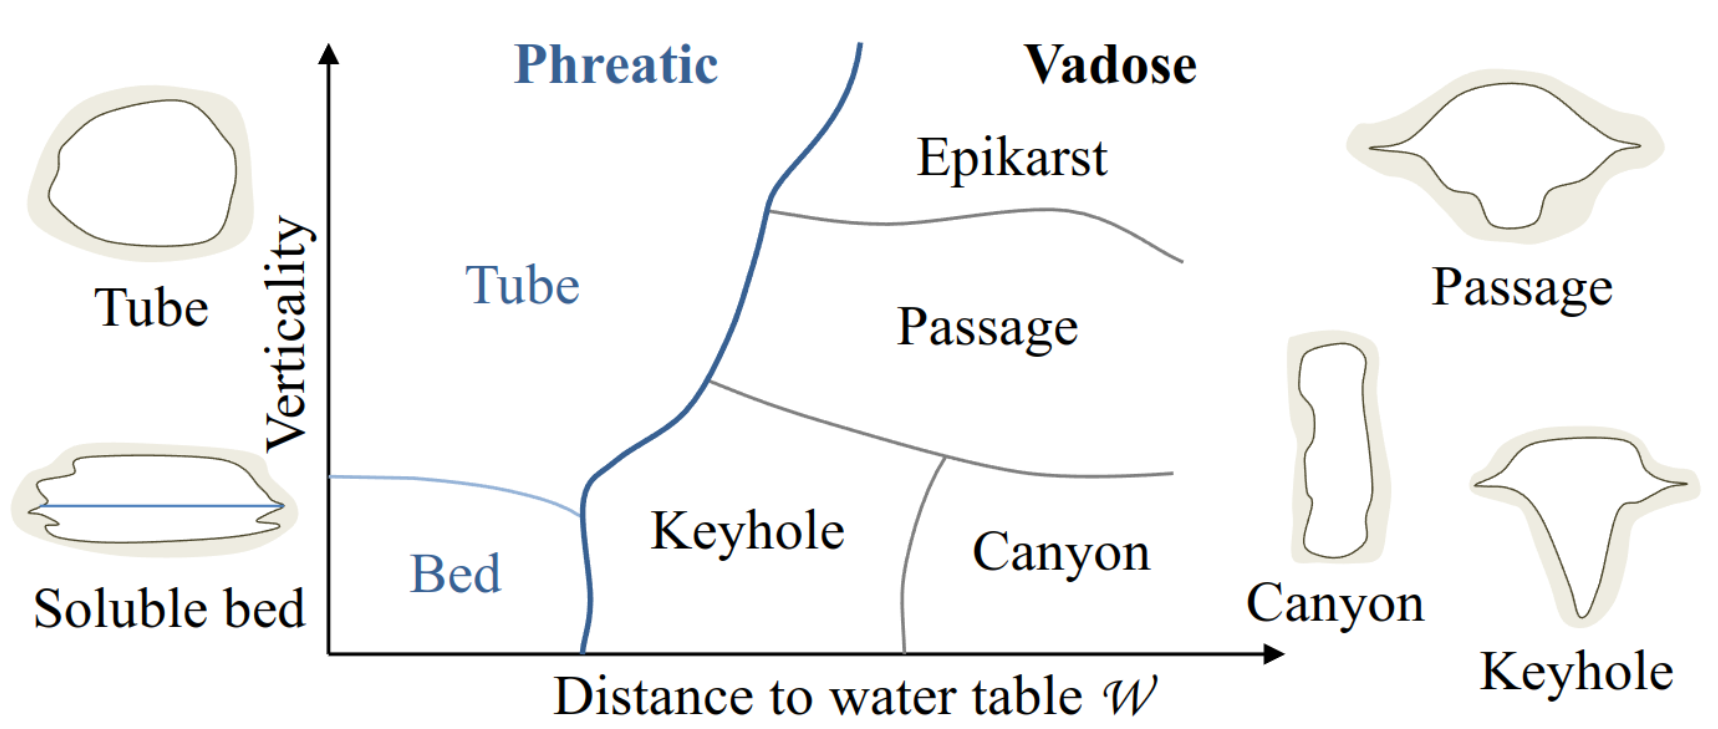
\includegraphics{KarstClassificationParis}
    \caption{Classification of tunnel shapes}
    \label{fig:karsts_tunnel-classif}
\end{figure}

\section{User Control}
\label{sec:karsts_user-control}
- Importance of keeping user control \\
** Shape of a karst is close to randomness \\
** Want to be predictible \\
- Manipulation of control points \\
** Source \\
** Sink \\
- Paths tortuosity \\
- Inclusion of soil properties in the formation of paths, using the gradient of: \\
** Humidity, \\
** Porosity \\
- Real-time editing \\
** Allows for precise manipulation \\
- ...

\section{Results}
\label{sec:karsts_results}
- ... 

\section{Conclusion}
\label{sec:karsts_conclusion}
- ...

\part{Erosion Simulation}

\chapter*{Abstract}
- Work carried out at the beginning of the thesis \\
- Representation choice still uncertain \\
- Search for abstraction of the representation \\
** Drives the generalization of the erosion system


\graphicspath{ {./Chapter 3/figures/erosion/}{./Chapter 3/figures/terrain_representations/}{./Chapter 3/results/}{./Chapter 3/otherPapersRepro/} {./Chapter 3/images/erosion_processes/}}

\newcommand{\referenceExemple}[1] {\textit{\cref{tab:erosion-result_figures}: #1}}
\newcommand{\addingFiguresToCell}[4]{%
        \autofitgraphics[width=0.2\textwidth]{#1}
        \autofitgraphics[width=0.2\textwidth]{#2}
        \ifx\relax#3\relax
        \else
            \autofitgraphics[width=0.2\textwidth]{#3}
        \fi
        \ifx\relax#4\relax
        \else
            \autofitgraphics[width=0.2\textwidth]{#4}
        \fi
}

% The columns :
% Name & Results & Terrain representation & Dimensions & particles / iteration & iterations & particle radius & coefficient of restitution & particle density & capacity factor & erosion factor & deposition factor & Velocity field & computation time
\newcommand{\exampleCoastal}{
Coastal & \addingFiguresToCell{Coastal_1.png}{Coastal_2.png}{Coastal_3.png}{} & \densityVox & 100x100x30 & 10 & 80 & 3 & 5 & 0.1 & 500 & 10.0 & 5.0 & 0.5 & Uniform & 0.5
}
\newcommand{\exampleGlacier}{
Glacier & \addingFiguresToCell{Glacier1.png}{Glacier2.png}{Glacier3.png}{Glacier4.png} & \heightmap & 100x100 & 20 & 80 & 3 & 10 & 0.1 & 500 & 1.0 & 1.0 & 1.0 & None & 0.8
}
\newcommand{\exampleLandslide}{
Landslide & \addingFiguresToCell{Glacier_2_1.png}{Glacier_2_2.png}{Glacier_2_3.png}{Glacier_2_4.png} & \heightmap & 100x100 & 20 & 200 & 10 & 2.5 & 0.2 & 500 & 0.1 & 1.0 & 1.0 & None & 4
}
\newcommand{\exampleHydraulic}{
Rain & \addingFiguresToCell{Hydraulic1.png}{Hydraulic3.png}{Hydraulic5.png}{Hydraulic7.png} & \heightmap & 100x100 & 20 & 100 & 10 & 1.0 & 1.0 & 1000 & 10.0 & 2.5 & 0.3 & None & 4.0
}
\newcommand{\exampleKarstBinary}{
Karst & \addingFiguresToCell{KarstBinaryWithMarchingCubes1.png}{KarstBinaryWithMarchingCubes2.png}{KarstBinaryWithMarchingCubes3.png}{KarstBinaryWithMarchingCubes5.png} & \binaryVox & 100x100x50 & 2 & 1000 & 40 & 5 & 0.5 & 500 & 10.0 & 5.0 & 0.5 & Uniform & 20
}
\newcommand{\exampleKarstBinaryStrata}{
Karst & \addingFiguresToCell{KarstWithStrataNoise1.png}{KarstWithStrataNoise2.png}{KarstWithStrataNoise3.png}{KarstWithStrataNoise4.png} & \binaryVox & 100x100x50 & 2 & 80 & 3 & 10 & 0.1 & 500 & 10.0 & 5.0 & 1.0 & Uniform & 0.8
}
\newcommand{\exampleLabyrinthOF}{
Glacier & \addingFiguresToCell{LabyrinthOpenFOAM1.png}{LabyrinthOpenFOAM2.png}{LabyrinthOpenFOAM3.png}{LabyrinthOpenFOAM4.png} & \densityVox & 100x100x40 & 2 & 80 & 3 & 10 & 0.1 & 500 & 1.0 & 1.0 & 1.0 & SIMPLE\cite{Caretto1973} & 0.8
}
\newcommand{\examplePipes}{
Tunnel & \addingFiguresToCell{Pipes01.png}{Pipes05.png}{Pipes09.png}{Pipes11.png} & \densityVox & 100x100x50 & 1 & 100 & 100 & 2.5 & 0.1 & 500 & 1.0 & 1.0 & 1.0 & None & 0.8
}
\newcommand{\exampleRiver}{
River & \addingFiguresToCell{River1.png}{River2.png}{River3.png}{River4.png} & \heightmap & 100x100 & 5 & 100 & 50 & 1.5-5 & 0.5 & 900 & 0.1 & 1.0 & 1.0 & None & 2.5
}
\newcommand{\exampleRiverTwo}{
River & \addingFiguresToCell{River_2_1.png}{River_2_2.png}{River_2_3.png}{River_2_4.png} & \heightmap & 100x100 & 5 & 100 & 50 & 1.5-5 & 0.5 & 900 & 0.1 & 1.0 & 1.0 & None & 2.5
}
\newcommand{\exampleRiverWater}{
\makecell{River
(with water
level)} & \addingFiguresToCell{RiverWater1.png}{RiverWater2.png}{RiverWater3.png}{RiverWater4.png} & \heightmap & 100x100 & 5 & 100 & 50 & 1.5-5 & 0.5 & 900 & 0.1 & 1.0 & 1.0 & None & 2.5
}
\newcommand{\exampleRiverObstacle}{
\makecell{River 
with obstacle} & \addingFiguresToCell{RiverWithObstacle1.png}{RiverWithObstacle2.png}{RiverWithObstacle4.png}{RiverWithObstacle6.png} & \heightmap & 100x100 & 5 & 100 & 50 & 1.5-5 & 0.5 & 900 & 0.1 & 1.0 & 1.0 & None & 2.5
}
% \newcommand{\exampleWaterCurrents}{
% Underwater & \addingFiguresToCell{WaterCurrent1.png}{WaterCurrent2.png}{WaterCurrent4.png}{WaterCurrent6.png} & \heightmap & 100x100 & 10 & 100 & 50 & 2.5 & 0.9 & 1000 & 1.0 & 1.0 & 1.0 & \cite{Stam2003} & 4
% }
\newcommand{\exampleWaterCurrents}{
Underwater & \addingFiguresToCell{WaterCurrent1.png}{WaterCurrent2.png}{WaterCurrent4.png}{WaterCurrent6.png} & \heightmap & 100x100 & 10 & 100 & 50 & 2.5 & 0.9 & 1000 & 1.0 & 1.0 & 1.0 & [Stam2003] & 4
}
% \newcommand{\exampleWindErosion}{
% Wind & \addingFiguresToCell{WindErosion1.png}{WindErosion2.png}{WindErosion4.png}{WindErosion5.png} & \densityVox & 100x100x50 & 0.2 & 100 & 10 & 1.5 & 0.9 & 1.5 & 1.0 & 1.0 & 1.0 & \cite{Paris2019b} & 0.5
% }
\newcommand{\exampleWindErosion}{
Wind & \addingFiguresToCell{WindErosion1.png}{WindErosion2.png}{WindErosion4.png}{WindErosion5.png} & \densityVox & 100x100x50 & 0.2 & 100 & 10 & 1.5 & 0.9 & 1.5 & 1.0 & 1.0 & 1.0 & [Paris2019] & 0.5
}
\newcommand{\exampleVolcano}{
Volcano & \addingFiguresToCell{Volcano_2_1.png}{Volcano_2_2.png}{Volcano_2_3.png}{Volcano_2_4.png} & \densityVox & 100x100x40 & 50 & 150 & 30 & 1.0 & 5.0 & 2000 & 1.0 & 1.0 & 5.0 & None & 0.8
}
\newcommand{\exampleMeanders}{
Meanders & \addingFiguresToCell{meanders_base.png}{meanders_fin.png}{}{} & \implicit & N/A & N/A & 10 & 20 & 5.0 & 1.0 & 1000 & 1.0 & 1.0 & 1.0 & $^{(1)}$ & 1
}


\chapter{Erosion simulation}
\label{chap:erosion}

\teaser {
	\autofitgraphics{teaser.pdf}
	\centering
	\caption{Applying shading and textures on the generated geometry can produce a plausible aspect of a coast eroded by waves on a long timespan, or a desertic landscape eroded by wind, or a mountainous area flatten by thermal erosion.}
	\label{fig:erosion-closerImage}
}

\abstract
% - Work carried out at the beginning of the thesis 

% - Representation choice still uncertain 

% - Search for abstraction of the representation 

% ** Drives the generalization of the erosion system

In this chapter, we present a novel particle-based method for simulating erosion on various terrain representations, including height fields, voxel grids, material layers, and implicit terrains. Our approach breaks down erosion into two key processes (terrain alteration and material transport) allowing for flexibility in simulation. We utilise independent particles governed by basic particle physics principles, enabling efficient parallel computation. For increased precision, a vector field can adjust particle speed, adaptable for realistic fluid simulations or user-defined control. We address material alteration in 3D terrains with a set of equations applicable across diverse models, requiring only per-particle specifications for size, density, coefficient of restitution, and sediment capacity. Our modular algorithm is versatile for real-time and offline use, suitable for both 2.5D and 3D terrains.
\pagebreak

\minitoc

\section{Introduction}
Automated terrain generation is a key component of natural scene digital modelling for animated movies and video games. A standard approach is to first generate a base terrain geometry using noise to define the height on the input domain \cite{Musgrave1989, Olsen2004, Roudier1993}, the result will most likely lack realism and feel synthetic. Erosion simulation algorithms are applied, to simulate thousands of years of ageing by reproducing physical phenomena (i.e. effects of the rain, wind, and running water erosion agents) affecting the terrain making it more believable \cite{Stachniak2005, Smelik2009, Galin2019}.

The process of terrain alteration caused by the effect of water, air, or any other element, natural or not, over time is usually performed in three steps \cite{Neidhold2005}: \textbf{detachment} (pieces of the ground of variable dimensions, ranging from complete ledges to grains of sand, are removed from the terrain depending on the simulated meteorological phenomenon), \textbf{transport} (pieces of ground fallen from their initial position are moved to a different one such as a cornice falling down a slope or a grain of sand thrown into the air), and \textbf{deposition} (transported pieces of land are accumulated at a new part of the landscape). Various phenomena can cause these alterations: \textbf{thermal erosion} (bursting of rocks caused by expansion of water under frost, then falling of debris to the bottom of a slope), \textbf{hydraulic erosion} (detachment caused by the impact of water particles on surfaces and the transport of sediments by the flow of runoff), \textbf{wind erosion} (fine particles carried away in the wind and hit surfaces on their way, creating new fine particles which then also fly away), \textbf{chemical erosion} (chemical decomposition of rocks caused by rainwater or other fluids), other exceptional phenomena such as avalanches, animals, lightning, etc... modify the terrain \cite{Cordonnier2017a, Argudo2020, Cordonnier2018, Cordonnier2017b,Cordonnier2023}.

\begin{figure*}
\centering
\autofitgraphics{pipeline.png}
\caption{Our method requires a base geometry, a small number of parameters for the particles and the medium used for the erosion simulation. It can be easily adapted to be compatible with different mediums and terrain representations.}
\label{fig:erosion-pipeline}
\end{figure*}

In practice, the core idea to simulate erosion is to add or remove material from the terrain at given positions on the interface between the terrain and fluid eroding it (e.g. air or water). Hence, the two major problems to tackle are: how to locally alter the terrain geometry for material detachment and deposition and where to perform these alterations given the properties of the environment (terrain slope, fluid density and velocity).
A terrain is more than often represented in 2.5D using a 2D image called a heightmap whose greyscale values define terrain elevation. While being the major terrain representation, only a limited number of environments can be modelled. Indeed, natural landscapes are intrinsically 3D (overhangs, cavities or geological structures such as arches or goblins), this is particularly true for underwater environments generation. Alternate representations such as voxel grids, material layers or implicit surfaces can be used. A wide variety of methods have been proposed to simulate natural erosion phenomena on heightmaps as the partial differential equations to model erosion can be discretised and solved in 2D and the material detachment and deposition at a given point of the terrain surface can be easily performed by elevating or lowering the ground level i.e. changing locally pixel intensities.
For volumetric representations, the alteration of the terrain is not as trivial.
To define where to perform the erosion process, the local slope variations are more than often used combined with eroding medium information. This fluid can be simulated using particle systems, Smoothed Particle Hydrodynamics (SPH) \cite{Kristof2009} or approximated using a simple vector field.
Proposed methods offer a specific erosion effect tailored to a single terrain representation and fluid simulation.

In this work, we propose an approach to simulate a large part of the geomorphological and meteorological phenomena present in the literature of terrain generation (including 3D and volumetric effects). We introduce a generalised algorithm performing the three stages of erosion on surface and volume representations alike, and expose very few intuitive parameters to be adjusted by the user (\cref{fig:erosion-pipeline}).
We propose to tackle separately the material variation and the fluid simulation. Our method relies on a particle system to simulate eroding agents, each thrown particle will collide with the terrain, perform terrain alteration at the collision point and transport material along its path.
Their motion is computed using simple particle physics accounting for the medium density and particle properties (buoyancy and gravity forces). We consider each particle as independent, hence, they do not interact with each other, no collision detection or response. This simplification allows for efficient parallel computation.
When more accuracy or control is needed, we propose to provide a vector field used to modify the particle speed at each time step. The nature of this vector field is flexible, it can be computed using a more or less accurate fluid simulation (SPH, FLIP,...) or be manually defined by the user. We propose a particle-based strategy for material alteration that can be applied on surface and volumetric representations.

The main contributions of this chapter are:
\begin{Itemize}
\Item{} a generalised particle-based algorithm performing the three
stages of erosion on surface and volume representations,
\Item{} decoupling the erosion system from the fluid simulation, making the process more flexible in its usage and implementation and opening the door for richer effects that can easily be produced.
\end{Itemize}
% -----------------------------------------------------------------

% \section{Erosion}
% Erosion is the complex, gradual process through which natural forces such as water, wind, ice, and gravity wear away soil, rock, and sediment, transporting these materials across the landscape and leading to significant changes in topography and landform structure over time. This process, fundamental to both natural and human-modified environments, involves several interacting factors, including the type and composition of surface material, climate conditions (such as precipitation, temperature fluctuations, and wind intensity), topography (including slope steepness and aspect), and the presence of vegetation.

% Studying erosion is essential across numerous fields due to its impact on landscapes, ecosystems, infrastructure, and resource sustainability. In agriculture, for example, erosion poses a direct threat to soil fertility and crop productivity, driving the need for conservation practices that retain topsoil and prevent land degradation. In civil and environmental engineering, erosion control measures are fundamental to maintaining the stability of roads, bridges, and coastal structures, safeguarding both urban and rural infrastructure. Similarly, urban planning incorporates erosion management into green infrastructure and stormwater systems to protect densely populated areas from soil loss and water damage. Ecologically, erosion shapes habitat stability and biodiversity, affecting riverine, forest, and coastal ecosystems; as a result, restoration efforts are vital to sustain healthy landscapes and support species diversity. In water resource management, erosion control is integral to preventing sedimentation, preserving water quality, and managing flood risks, which are essential for both environmental health and human safety. Within climate science, erosion is studied for its role in the carbon cycle, land degradation, and desertification, as it influences carbon release and soil loss in vulnerable areas. Erosion is also a key focus in natural disaster risk assessment, where slope stability and riverbank management are crucial for preventing landslides and floods that could endanger communities. Furthermore, in mining and resource extraction, erosion control mitigates environmental damage by supporting ecosystem recovery and reducing sediment pollution in surrounding areas. [ADD CITATIONS FOR EACH FIELD].

% The effects of erosion extend beyond simple landscape alteration. They play a central role in soil formation, nutrient cycling, and the distribution of sediments in various ecosystems.

% The main problem with studying erosion is the large amount of factors to take into account in the process. When studying erosion, a range of interconnected properties must be considered to understand its causes, rates, and impacts. Soil and rock characteristics such as texture, structure, cohesion, permeability, and organic matter content influence how easily soil and sediment detach and are transported. Climate factors like rainfall intensity, temperature fluctuations, wind speed, and seasonal changes impact erosion by affecting soil moisture and stability. Slope gradient, river length, elevation, and drainage patterns affects how water flows and gathers momentum, directly influencing erosion potential. Hydrological factors like surface runoff, infiltration rate, groundwater flow, and wave action are critical in understanding how water drives erosion in riverine and coastal environments.

% Biological influences include vegetation cover, root density, and plant types, which stabilize soil, while animal activities like burrowing can increase erosion susceptibility. Human activity, such as agriculture, deforestation, urbanization, and mining, significantly accelerates erosion by disturbing soil and removing natural vegetation. Geological properties like soil depth, rock layering, and prior erosion events, along with chemical characteristics such as mineral composition and soil acidity, also shape erosion patterns, influencing how landscapes respond to environmental forces. Temporal factors, including the duration of exposure, rate of soil formation, seasonal cycles, and the frequency of intense weather events affect erosion rates over time, leading to varying erosion impacts across regions and ecosystems. These properties collectively provide a comprehensive foundation for understanding and managing erosion processes across diverse landscapes.

% Due to the large amount of properties to take into account, each domain uses a subset of the factors, with more or less simplifications in the erosion model. Depending on the use case, the analysis of erosion effects may vary largely. [ADD EXAMPLE OF FIELDS THAT STUDY EROSION THAT HAVE INSTANTANEOUS EFFECTS LIKE LANDSLIDES AND FIELDS THAT USE MILLIONS OF YEARS LIKE TECTONIC ACTIVITY].

% In procedural terrain generation, simulating erosion based on soil and rock characteristics (like texture, cohesion, and permeability) allows the algorithm to mimic how different materials break down and redistribute under various conditions. For example, regions with sandy or loosely cohesive soils can be programmed to erode more rapidly, while rocky, cohesive areas remain more stable.

% Incorporating climate factors (rainfall, wind, and temperature) helps to model how landscapes evolve in different biomes such as dry, windy deserts versus lush, wet valleys. Simulating topographic influences like slope gradient and drainage patterns enables the formation of natural-looking valleys, cliffs, and river networks, while accounting for hydrological factors like runoff and groundwater flow creates realistic water paths and sediment deposits.

% Procedural algorithms can also use biological factors to define erosion resistance based on vegetation cover, with densely vegetated areas exhibiting slower erosion rates and barren regions eroding faster. Including human activity effects, such as altered runoff or deforestation, allows for terrain that mirrors landscapes influenced by development or agriculture, adding further realism. Finally, using temporal properties to simulate seasonal erosion and landscape changes enables the terrain to evolve naturally over time, creating dynamic environments where erosion patterns shift as weather and vegetation change.





\section{State of the art}
\label{sec:erosion-state_of_the_art}
In this section, we first a subset of the major simulated phenomena used to erode terrains, then we will cover the different fluid simulation algorithms used in procedural terrain generation. We highlight the fact that, in the literature, a specific erosion method tailored to a given terrain representation is proposed for given phenomena which might lead to limitation in term of terrain modeling. Indeed, changing representation costs information and precision loss.

% \subsection{Terrain representations}

% Terrain refers to the physical features and configuration of a specific area of land. It includes the elevation, slope, and the overall topography, such as mountains, valleys, and plains. Terrain is often used to describe the surface characteristics of the land, focusing on the natural contours and the geographical aspects that define a region's physical form.

% While the term "terrain" describes the physical characteristics of land, it does not include the natural elements that shape an area's identity. Elements like vegetation, water bodies, and climatic conditions, such as snow cover, are essential to how we perceive and understand a landscape. Therefore, when discussing procedural generation in virtual environments, "landscape generation" is a more fitting term, as it integrates these natural elements along with the topographical features.

% In addition to "terrain generation," other terms such as "landscape generation," "world generation," and "environment generation" can be used to describe the creation of virtual landscapes. These terms are interchangeable and can all refer to the process of generating physical terrain along with natural and artificial elements. However, by convention and for simplicity, the term "terrain generation" is most commonly used in the field. Despite its original focus on the physical features of the land, "terrain generation" has evolved to encompass a broader range of environmental elements, making it a convenient and widely accepted term for describing the comprehensive process of creating virtual environments.

% A terrain can be represented in various ways, each of them suited for a given application of which we give an brief overview, more details can be found in \cite{Galin2019}.

% \subsubsection{Elevation models}

% \begin{figure}
%     \centering
%     \autofitgraphics[width = 0.8 \linewidth]{elevation_representation.png}
%     \caption{Elevation functions}
%     \label{fig:erosion-elevation-representation}
% \end{figure}

% Elevation models are a fundamental approach in terrain representation, widely used in procedural generation due to their simplicity and efficiency. These models define the terrain as a function $h : \R^2 \to \R$, where each point in a 2D plane is mapped to an elevation value. This approach is particularly effective for representing terrains where the elevation is the only varying factor, such as hills, valleys, and plateaus, and it is best suited for terrains without complex 3D features like overhangs or caves. While we visualize elevation models in three dimensions, they are mathematically considered two-dimensional functions. In the domain of terrain generation, we will name them 2.5D models.

% Elevation models are widely used in industries where large-scale terrain representation is crucial. In video games, they provide the foundation for creating vast open-world environments. In geographic information systems (GIS) and remote sensing, height fields are used to represent real-world terrain data, offering a practical means of visualizing and analyzing geographical features. The ability to manipulate and control terrain features procedurally makes elevation models a common choice for applications that require efficient terrain generation and rendering.

% They offer a powerful method for representing terrains in procedural generation, combining simplicity with flexibility. While they have limitations in representing complex 3D structures, their efficiency and compatibility with existing algorithms make them indispensable in a variety of applications.

% \subsubsubsection{Implicit height fields}

% \begin{wrapfigure}{L}{0.4\textwidth}
%     \autofitgraphics[width=\linewidth]{primitives_representation.png}
%     \caption{Primitives composition}
%     \label{fig:erosion-primitives-representation}
% \end{wrapfigure}

% Implicit height fields represent the terrain as a mathematical function that provides a height value at any given point in the domain. These functions can be procedural or closed-form expressions, allowing for compact storage and infinite precision in theory. The elevation function allows for easy manipulation of terrain features, making it ideal for generating terrains that require smooth, continuous surfaces. However, the primary disadvantage is the computational complexity involved in evaluating the function, especially for large or highly detailed terrains. The challenge lies in constructing functions that can realistically represent large-scale terrains with complex landforms.

% \subsubsubsection{Discrete height fields}
% Discrete height fields, or explicit height fields, are one of the most prevalent methods for terrain representation. These models consist of a 2D grid where each cell contains a height value, representing the elevation at that point. Height fields are particularly advantageous because they are simple to implement and are directly compatible with many rendering techniques and hardware, but also due to their closeness with image processing, a domain studied for many decades now.

% The main advantage of height fields is their ability to handle large datasets efficiently, providing a balance between memory usage and detail. However, they are limited by their inability to represent terrains with overhangs or caves, as each point on the grid can only hold a single elevation value. Additionally, height fields often require interpolation methods, such as bi-linear or bi-cubic interpolation, to reconstruct a continuous surface from the discrete grid points. 

% \subsubsection{Volumetric models}

% \begin{figure}
%     \centering
%     \autofitgraphics[width = 0.8 \linewidth]{volumetric_representation.png}
%     \caption{Volumetric functions}
%     \label{fig:erosion-volume-representation}
% \end{figure}

% Volumetric models represent a more complex approach to terrain modeling, allowing for the depiction of 3D features that go beyond the simple surface-based representation provided by elevation models. These models capture not only the surface of the terrain but also its internal structure, making them ideal for representing terrains with overhangs, caves, and other subsurface features. 

% Volumetric models, including layered materials, voxel grids, and implicit models, are essential in applications where terrain complexity and detail are primordial. In geological simulations, these models allow for accurate representation of subsurface structures and processes. Voxel models are widely used in games that require dynamic terrain deformation, providing a rich interactive environment for players. Implicit models are favored in situations where smooth, continuous surfaces are needed [FIND OTHER USE CASES].

% \subsubsubsection{Implicit volumetric models}
% Implicit volumetric models describe the terrain's shape and features using an implicit function. The terrain is represented by a mathematical function $f: \R^3 \to \R$ that determines the terrain surface by evaluating to an isovalue, often zero. This function provides a continuous representation of the terrain, with points inside the terrain returning positive values and while points in the air evaluate to negative values. It allows for the seamless representation of complex terrain features, including caves, overhangs, and varying geological structures, which are impossible to represent with  elevation models.

% One of the key advantages of implicit models is their ability to produce smooth surfaces without the need for discrete polygonal meshes, which can result in realistic and natural-looking terrains. However, the computational complexity of evaluating the implicit function, especially for large terrains, can be a significant drawback. Additionally, converting an implicit surface into a mesh for rendering can be challenging and resource-intensive. \cite{Araujo2015} 

% \subsubsubsection{Layered models}
% Layered models are a type of volumetric representation that encode different material layers within the terrain and are defined by a function $\mu : \R^3 \to \material$, where $\material$ denotes the material type at any given point in 3D space. This allows for a detailed representation of the terrain's internal composition, which can be crucial for applications requiring realistic geological simulations. Each layer is defined by its thickness or elevation, and multiple layers can be stacked to represent complex geological formations. These layers might include materials like bedrock, sand, soil, or water, each contributing to the overall structure of the terrain. Layered models are particularly useful in simulations that involve processes like erosion or sedimentation, where the interaction between different material layers affects the physical process.

% The primary advantage of layered models is their ability to represent a stratified terrain with distinct material properties, which can be manipulated individually. This makes them well-suited for simulations that require detailed geological accuracy. However, they are more complex to implement than simple elevation models and require additional computational resources to manage the interactions between layers. 


% \subsubsubsection{Voxel grid models}
% Voxel grids are a common method for representing 3D terrains in procedural generation, offering the ability to capture complex internal structures and features that are difficult or impossible to represent with surface-based models. In a voxel grid, the 3D space is divided into a regular grid of small, cube-shaped elements called voxels (volumetric pixels). Each voxel holds information about the material or properties of the terrain at that specific point in space. This approach allows for detailed modeling of features such as caves, tunnels, overhangs, and intricate underground networks. The regular grid structure allows for the use of image processing-oriented algorithms.

% There are three primary types of voxel grids used in terrain representation: binary voxel grids, material voxel grids and density voxel grids. Each has distinct characteristics, advantages, and limitations, making them suitable for different applications. 

% \subsubsubsubsection{Binary voxel grids}
% Binary voxel grids are the simplest form of voxel representation. In these grids, defined $f: \R^3 \to [0, 1]$, each voxel is either "filled" or "empty," representing the presence or absence of material. This binary state is typically represented by a 1 (filled) or 0 (empty). Binary voxel grids are straightforward to implement and require much less memory compared to more complex voxel representations, making them ideal for applications where the primary concern is whether a space is occupied or not.

% The simplicity of binary voxel grids is one of their main advantages. They are easy to understand and visualize, with each voxel requiring only a single bit of information to represent its state. Additionally, because only a binary state is stored, these grids can be memory-efficient when combined with compression techniques like Sparse Voxel Octrees (SVOs) \cite{Laine2010} or voxel Directed Acyclic Graphs (DAG) \cite{Villanueva2017,Careil2020}. The simplicity of the data structure also allows for quick processing, making binary voxel grids suitable for real-time applications where performance is required. However, the binary nature of these grids limits their ability to represent variations in material density or properties, or even smoothness, resulting in less detailed terrain models. This can lead to hard, blocky edges in the terrain, which may appear unnatural without additional smoothing or processing.

% \subsubsubsubsection{Material voxel grids}
% Material voxel grids, defined as $\mu: \R^3 \to \material$, are commonly used in applications where simple occupancy information is sufficient. For example, voxel-based games like Minecraft utilize material grids to create terrains composed of solid blocks with clear boundaries. These grids are also employed in scientific simulations where the primary concern is the presence or absence of materials, rather than detailed material properties.

% \subsubsubsubsection{Density voxel grids}
% Finally, density voxel grids allow each voxel to store a range of values, representing varying degrees of material presence with $f: \R^3 \to \R$. Instead of a simple discrete state, a density voxel grid assigns a continuous value to each voxel, which can represent material density, opacity, or other properties. This added complexity enables density voxel grids to represent subtle variations in terrain, such as gradual changes in material density or smooth transitions between solid and empty spaces, allowing for more realistic and natural-looking terrain models.

% % The use of density voxel grids results in soft transitions and smooth surfaces, reducing the blockiness typically associated with binary voxel grids. They are versatile and can represent not only solid terrain but also phenomena like fog, fluid densities, or temperature gradients. However, the increased detail and realism come at the cost of greater complexity. Density voxel grids require more memory and computational power, making them more challenging to implement and manage. The additional data and processing required can also lead to slower performance, particularly in real-time applications.

% Density voxel grids are often used in high-fidelity simulations where detail and realism are essential. They are found in applications such as medical imaging, scientific visualizations, and advanced terrain modeling for films and visual effects. These grids are also employed in procedural terrain generation systems that require smooth and natural transitions between different terrain features, such as caves, cliffs, and eroded landscapes.



\subsection{Erosion processes}
Driven by an array of natural forces and processes, erosion varies significantly across environments, from the intense carving of river valleys to the subtle reshaping of slopes in arctic regions. In this section, we present the primary types of erosion (thermal, hydraulic, and wind erosion) alongside other significant processes that contribute to landscape change.  
Each erosion type not only influences distinct terrain forms but also varies in applicability depending on terrain representation in simulations. Notably, not all erosion types are easily adaptable to all forms of terrain representation due to inherent limitations in data resolution and computational methods.

\subsubsection{Gravity-driven erosion}
Gravity-driven erosion encompasses processes that involve the downslope movement of soil, rock, or debris due to the force of gravity. These processes, including landslides and talus slope formation, play a crucial role in reshaping landscapes by redistributing materials across slopes, valleys, and cliffs, influencing terrain stability and morphology.


\subsubsubsection{Thermal erosion}
\AltTextImage{
    % \wrapFig{freeze-thaw.jpg}{0.25.}{fig:erosion-freeze_thaw}{Freeze-thaw process from \cite{Wang2017}}

    Freeze-thaw weathering, also known as frost wedging, frost shattering, or more simply thermal erosion in Computer Graphics, is a process that occurs when water infiltrates cracks and pores within rocks and then freezes (\cref{fig:erosion-freeze-thaw-example}). As the water freezes, it expands and exerts pressure on the rock, causing it to fracture and break apart over time. This cycle of freezing and thawing is especially prevalent in regions with large temperature variations between day and night or between seasons, such as alpine and polar climates. Over time, freeze-thaw weathering contributes to the breakdown of large rocks into smaller fragments, creating loose rock material that can accumulate and gradually move downslope.
}{freeze-thaw.jpg}{Freeze-thaw process \cite{Wang2017}.}{fig:erosion-freeze-thaw-example}{Freeze-thaw process}

Freeze-thaw weathering plays an important role in shaping landscapes, as it weakens rock faces and cliff edges, contributing to the formation of loose rock debris that eventually becomes part of other erosive processes, such as the development of talus slopes. This process, involving freeze-thaw cycles, can quickly fragment rock surfaces, with cumulative landscape impacts such as the formation of talus slopes observable over decades to centuries.

% \wrapFigR{talus.png}{}{}{} % {Mark A. Wilson (Department of Geology, The College of Wooster)}{fig:erosion-talus}
\AltTextImage{
    \subsubsubsection{Talus slopes}
    Talus slopes, also known as scree slopes, are accumulations of loose, angular rock debris at the base of cliffs, steep slopes, or mountainous areas. These slopes form as fragments of rock break off due to weathering processes such as freeze-thaw, and gravity pulls them downslope, where they accumulate in a cone-shaped deposit (\cref{fig:erosion-talus-example}). Talus slopes are common in high-altitude or cold regions where physical weathering of rock faces is intense, and they contribute to the visual ruggedness of mountainous landscapes. Formed by the accumulation of rock debris from higher elevations, talus slopes develop gradually as materials accumulate, influencing terrain over centuries.
}{talus.png}{Talus cones on north shore of Isfjord, Svalbard, Norway - Photo credit: Mark A. Wilson.}{fig:erosion-talus-example}{Talus cones on north shore of Isfjord, Svalbard, Norway}

% The procedural terrain generation domain blurs the definition of thermal erosion introduced by \cite{Musgrave1989}, simplifying it to a material stabilisation problem. 

\subsubsubsection{Landslides}
Landslides encompass a range of processes where rock, soil, or debris moves downslope due to gravity. These events vary in scale and speed, ranging from rapid, sudden rockfalls to slow, gradual soil creep (\cref{fig:erosion-landslides-processes} illustrate different landslide processes). They can be triggered by factors such as heavy rainfall, seismic activity, or thawing permafrost, which destabilise slopes and initiate movement. Key types of landslides include:

\AltTextImage{
    \begin{Itemize}
        \Item{} \textbf{Rockfalls:} Sudden detachment of rock from steep faces, often triggered by weathering, freeze-thaw cycles, or seismic activity, leading to rapid downslope movement. 
        \Item{} \textbf{Soil creep:} Slow, continuous downslope movement of soil and rock, caused by repeated cycles of expansion and contraction due to changes in moisture and temperature, often imperceptible over short timescales.
        \Item{} \textbf{Mudflows and debris flows:} Rapid flows of water-saturated soil and debris, typically triggered by heavy rainfall or snowmelt, which transport large volumes of material downslope in a short period.
    \end{Itemize}
}{earthflow-erosions.jpg}{Different landslide processes: soil creep, slump, lahar, mudflow, and rockfall. }{fig:erosion-landslides-processes}{Different landslide processes}

Landslides are a major force in landscape evolution, rapidly reshaping terrain and redistributing materials across slopes and valleys. Triggered by factors such as heavy rain or seismic activity, landslides can reshape landscapes almost instantaneously, though their frequency and impact may vary widely.

\smallConclusion

Realistic simulation of these effects can be achieved by applying multi-flow Computational Fluid Dynamics on the internal rock fragments or sediments, considering them as fluid particles with an evaporating viscosity \cite{Feng2024,Harmon2001,Lenaerts2009} or as inelastic frictional spheres \cite{Walton1993}, but at the cost of very high computation times.

\AltTextImage{
    In procedural terrain generation, however, freeze-thaw, talus slopes, and landslides are all similarly considered and generalised as "thermal erosion". The use of "thermal erosion" or "thermal weathering" in procedural generation, introduced by \cite{Musgrave1989}, is a misnomer initially used in opposition to "hydraulic erosion". However, the effect of freeze-thaw can be seen as a reduction in the ground resistance to detachment, as the critical shear stress is highly reduced in cold weather regions, while talus slopes and landslides involve finer soil particles or the mixing of liquid fluids, introducing viscosity into the system, resulting in a quite similar output \cite{Hudak2011}.
}{thermal-erosion-Olsen2004.png}{Left: initial fractal terrain; right: thermal erosion simulation from \cite{Olsen2004}.}{fig:erosion-thermal-Olsen2004}{\cite{Olsen2004}'s thermal erosion simulation}

\AltTextImage{
    Thermal erosion can be simulated by redistributing rock fragments or particles to accumulate at the base of cliffs or steep inclines, taking into account only the surface of the terrain. This effect can be achieved by applying gravity-based algorithms that allow loose materials to fall and settle, forming natural slopes of debris at the base of rocky terrain \cite{Musgrave1989,Jones2010}. Initially proposed for discrete height field terrain representations, the thermal erosion simulation proposed by \cite{Musgrave1989} and improved for GPUs by \cite{Jako2011} iteratively displaces a small amount of the height at each cell of the terrain and redistributes it to its direct neighbours if a repose angle is not satisfied (see \cref{fig:erosion-thermal-explained-Galin2019}, used in \cref{fig:erosion-thermal-Olsen2004}). 
    }{thermal-erosion-explained-Galin2019.png}{Layered terrain thermal erosion simulation iteratively distributeunstable material from a cell to its neighbours until all slopes satisfy a maximum repose angle $\theta$ \cite{Galin2019}.}{fig:erosion-thermal-explained-Galin2019}{Illustration of thermal erosion simulation on layered terrains}

\AltTextImage{
    \cite{Jones2010} adapts this definition of thermal erosion for density-voxel representations, and \cite{Benes2001} for layered representations. 
    The importance of keeping track of scree areas allows for more detailed modelling such as the addition of geometry of rock piles illustrated in \cref{fig:erosion-aperiodic-rocks-Peytavie2009a}, mimicking talus blocks at the bottom of a canyon \cite{Peytavie2009a,Paris2020}.
}{aperiodic-rocks-Peytavie2009a-s.png}{Procedural rock piles from \cite{Peytavie2009a}. }{fig:erosion-aperiodic-rocks-Peytavie2009a}{Procedural rock piles}

\subsubsection{Hydraulic erosion}
\begin{figure}
    \autofitgraphics[width = 0.8 \linewidth]{hydraulic_erosion.pdf}
    \caption[Hydraulic erosion is caused by the friction of water displacing sediments on a slope from intense water flow regions to calmer downstream areas]{Hydraulic erosion is caused by the friction of water displacing sediments on a slope from intense water flow regions to calmer downstream areas.}
    \label{fig:erosion-hydraulic-erosion}
\end{figure}

\AltTextImage{
    Hydraulic erosion is the process by which moving water dislodges and transports soil, sediment, and rock from the Earth's surface (\cref{fig:erosion-hydraulic-illustrated-Galin2019}). Occurring in multiple forms, including river-based, rainfall-induced, and coastal erosion, hydraulic erosion is driven by factors such as water velocity, volume, and surface composition. 
    }{hydraulic-process-Galin2019.png}{Hydraulic erosion  simulations uses water as a medium to move sediments from one position to another. }{fig:erosion-hydraulic-illustrated-Galin2019}{Illustration of hydraulic erosion simulation}

This process plays a primary role in reshaping landforms, forming valleys, river channels, and coastlines, and significantly contributes to sediment redistribution in terrestrial and coastal environments.

% \AltTextImage{
    \subsubsubsection{Fluvial erosion}

    Fluvial erosion is the process by which rivers and streams reshape the landscape by eroding, transporting, and depositing sediment. This phenomenon occurs as the kinetic energy of moving water exerts mechanical forces on the riverbed and banks, dislodging soil, rock, and sediment particles (\cref{fig:erosion-hydraulic-erosion}). The intensity of fluvial erosion is influenced by factors such as water velocity, discharge (volume of water flowing per unit time), channel slope, and the composition of the riverbed and banks.
% }{river_erosion.pdf}{The erosion on the river bank is the combination of two processes: the detachment of the bottom of the sides, then the break of the upper coasts.}{fig:erosion-river-erosion-profile}

In steep, fast-flowing sections of a river, higher water velocities generate turbulent flow, which increases the river's capacity to dislodge and carry large particles. These particles, including gravel and pebbles, collide with the riverbed in a process called abrasion, grinding and wearing down the bedrock over time. Additionally, water exerts direct hydraulic pressure, especially in areas where currents are swift, prying apart rocks and sediment through hydraulic action. This is especially effective in widening channels and undercutting banks.

Fluvial erosion processes contribute to the dynamic reshaping of river channels, forming distinct landforms such as V-shaped valleys, canyons, and river meanders. Over time, rivers naturally balance their erosive energy with sediment transport and deposition, forming floodplains where sediment is deposited during seasonal overflows. In meandering rivers, erosion typically occurs on the outer curves of bends, where flow velocity is highest, while sediment deposition takes place on the inner curves, forming point bars. This continual interaction between erosion and deposition drives the lateral migration of meanders, altering the river's course across the landscape. The river's competence, or its ability to transport particles of a certain size, depends on the flow's velocity and discharge. During periods of high flow, such as after heavy rainfall or snowmelt, rivers gain greater erosive power, enabling them to transport larger particles and increase their erosion rates. River systems reshape landscapes methodically over years to millennia, deeply engraving river paths and altering regional topographies.



\AltTextImage{
    \subsubsubsection{Rainfalls}
    % \wrapFig{rillsGullies.jpg}{0.25.}{fig:erosion-rills_gullies}{From \cite{Geertsema2010}}

    Rainfall-induced hydraulic erosion begins as raindrops strike exposed soil surfaces, causing splash erosion, where particles are dislodged and displaced by the impact of individual raindrops, creating tiny craters \cite{Valette2005,Li2024}. As rainfall accumulates and flows overland, it transitions into sheet erosion, where a thin layer of water, known as sheet flow, moves across the land surface. This process is often intensified on sloped terrain, where the water gains momentum as it descends, picking up and carrying loose particles downslope. Sheet erosion can remove a uniform layer of soil across a large area, gradually depleting soil fertility and weakening the structure of the soil surface.
}{rillsGullies.jpg}{Rill and gully erosion along the Chilcotin River \cite{Geertsema2010}.}{fig:erosion-rills_gullies}{Rill and gully erosion along the Chilcotin River}

On steep or prolonged slopes, sheet flow may concentrate into small channels, initiating rill erosion \cite{Gatto2000}. Rills are narrow, shallow channels that cut into the soil as water flow converges, carving miniature stream-like paths down the slope visible in \cref{fig:erosion-rills_gullies}. As rills deepen and widen, they can evolve into larger channels in a process called gully erosion, where channels become deep and wide enough that normal agricultural or natural processes cannot easily repair them. Gullies disrupt the landscape, fragmenting ecosystems, and accelerating the removal of topsoil.

The extent of erosion depends on factors such as rainfall intensity and duration, soil type, vegetation cover, and slope steepness. Sandy soils, for instance, are more prone to erosion due to their low cohesion, whereas clay-rich soils, while more resistant to initial splash erosion, are highly susceptible to rill and gully formation once water begins to concentrate. Splash erosion and sheet erosion can cause significant soil degradation and landscape changes over months to decades.

\smallConclusion

Hydraulic erosion simulation dominates procedural terrain work because it produces large, coherent landforms and can be simulated efficiently with surface-based models using simple rainfall fields.
% Hydraulic erosion is the main focus of study in terms of erosion for terrain generation as its effects on the surface of terrains are visible on a large scale and are the most stable as we consider a constant amount of rain at every point.

In procedural terrain generation, fluvial erosion is focused on the generation of rivers and cascades defined as feature-curves \cite{Emilien2015}. First, the path of the river is drawn either by the user \cite{Hnaidi2010} or through simulation \cite{ParisThesis}. Second, the shape of the rivers' beds are modelled \cite{Genevaux2013}. It is then finally possible to provide a geometric representation of the water surface to take into account flow rate, depth, obstacles, and user-defined details \cite{Peytavie2019}.

The computation of rivers' properties is defined by understanding the flow of water, which is directly related to the amount of rainfall at each point of the terrain \cite{Kelley1988}, then approximated by simplified Shallow Water modelling \cite{Mei2007}, but is mainly achieved in acceptable computation time by considering all rivers as a drainage network, an oriented graph of rivers as introduced in \cite{Roudier1993}. Recent works focus on the acceleration of the computation of these graphs and the drainage area associated at each point \cite{Cordonnier2016,Schott2023}.

In most works, the amount of water falling at each point of the terrain can be taken into account. However, this strategy is divided among works that consider that rain falls uniformly on the whole terrain or using a random noise function, that rain is more present in regions of high altitude \cite{Neidhold2005}, or can use a more accurate weather simulation to define areas more prone to rainfall \cite{Wojtek2022}.

As the motion of water is easier to model on the surface of the terrain, almost all algorithms consider the terrain with a 2.5D representation. On a large scale, this assumption is beneficial but limits their scope to this type of representation, making them unavailable to volumetric models. Particle-based methods are then proposed to overcome this issue for smaller-scale terrains, using 3D Eulerian fluid simulations on voxel terrain representations \cite{Benes2006} or Lagrangian simulations on TIN terrains \cite{Kristof2009}, at the expense of much higher computational time.

\AltTextImage{
    \subsubsection{Chemical erosion and caves}

    Chemical erosion, also known as chemical weathering, involves the chemical reactions between water and rock that lead to the dissolution and alteration of minerals within the rock. This process is especially significant in river and coastal environments, where water, often containing dissolved carbon dioxide, interacts with rocks such as limestone and dolostone to form weak carbonic acid. This acid reacts with carbonate minerals, gradually breaking down the rock structure through a process called dissolution. Over time, this breakdown weakens rock formations, making them more susceptible to mechanical erosion by water.
}{seaCaveArch.jpg}{Akun Island basalt sea cave - Photo credit: Steve Hillebrand.}{fig:erosion-corrosion-erosion}{Akun Island basalt sea cave}

Chemical erosion is particularly influential in the formation of karst landscapes, where the dissolution of carbonate rocks creates unique features such as caves, sinkholes, and underground drainage systems. As acidic water seeps into fractures within the rock, it slowly enlarges these cracks, leading to the creation of hollow spaces and intricate cave networks. In addition to carbonic acid, other dissolved ions, such as sulphur and organic acids, can also contribute to the chemical weathering of rocks in various environments. The dissolution of soluble rocks such as limestone forms extensive karst landscapes, including networks of underground caves, over thousands to millions of years.

Sea caves can form through the mechanical force of hydraulic action as waves continuously impact the shore. These sea caves develop along coastlines with cliffs, where wave energy focuses on weak points in the rock, such as fractures or softer rock layers. Over time, the pressure from waves and tides pries apart rock fragments, carving out hollow spaces within the cliffside or even a whole arch as presented in \cref{fig:erosion-corrosion-erosion}. Formed by the erosive power of waves against rock cliffs containing zones of weakness, development can be observed over hundreds to thousands of years.

% This hydraulic action often works in conjunction with other processes, such as abrasion, where sediment carried by waves further grinds down the rock surfaces. Sea caves are commonly found in areas with high tidal energy, with examples such as the Blue Grotto in Malta and the sea caves along California's coastline.
In desert environments, caves can also form through aeolian erosion, where wind-driven sand particles abrade rock surfaces. These aeolian caves are typically found in sandstone or other softer rocks, where strong, consistent winds gradually wear away the rock. Unlike chemical or hydraulic caves, aeolian caves are usually shallower and smaller, as the erosive force of wind is less powerful than water or acid-driven processes. However, these caves add unique features to desert landscapes, creating sheltered hollows that sometimes serve as habitats for desert wildlife. Created by wind erosion primarily in softer rock formations, these caves can develop over centuries, depending on the consistency and strength of wind.

% An example of aeolian caves can be seen in the Navajo Sandstone formations of the southwestern United States, where wind erosion has carved intricate cave-like recesses and arches.
\smallConclusion

\AltTextImage{
    In procedural terrain generation, chemical erosion has been rarely studied, as this interaction mostly occurs in shallow to deep waters and requires a volumetric representation, while most terrain generation algorithms are tailored to aerial landscapes and are limited by 2.5D representations. However, as visible in \cref{fig:erosion-corrosion-Wojtan2007}, using 3D cellular automata can provide an explicit representation of this effect \cite{Menshutina2020,Wojtan2007} (and can be extended to a simulation of coastal erosion \cite{Hawick2014}). 
}{corrosion-Wojtan2007.png}{\cite{Wojtan2007} simulates chemical erosion on a regular grid. }{fig:erosion-corrosion-Wojtan2007}{\cite{Wojtan2007}'s corrosion simulation}

\AltTextImage{
    An approximation of this phenomenon is proposed in \cite{Beardall2007,Jones2010} on voxel grids by considering that the most vulnerable voxels of the terrain are the ones that have the most neighbours with air voxels, in a very similar manner to the computation of voxel-grid ambient occlusion (\cref{fig:erosion-spheroidal-weathering-Jones2010}). The simulation of sea caves for implicit terrains has been proposed by \cite{Paris2018} by considering a resistance function in the bedrock, usually a function of height, and adding spherical holes in the construction tree at the least resistant areas of the terrain. The inverse percolation method enables the simulation to dig longer cavities, resembling coastal karsts.
}{spheroidal-weathering-Jones2010.png,spheroidal-weathering-result-Jones2010.png}{Top: spheroidal weathering proposed in \cite{Jones2010} on voxel grids iteratively removes most exposed voxels (red). Bottom: modulating exposition with a resistance map (red/green curve) creates specific weathering patterns. }{fig:erosion-spheroidal-weathering-Jones2010}{\cite{Jones2010}'s spheroidal weathering}

% \AltTextImage{
%     The generation of complete karst networks has been studied in different domains, such as hydrogeology, where the generation of conduits based on the hydrologic network and soil properties allowed the generation of the first examples of karst systems \cite{Jaquet2004,Pardo2012,Pytel2015}. However, these methods do not allow user control and the computation time is unfit for terrain generation. More recently, \cite{Paris2021} proposed to describe the karst network as a graph whose nodes are sampled points in the terrain and for which the shortest path (using soil resistance as the metric) between each point provides the path of each tunnel in the network. An improved algorithm, with more geological parameters, proposes more geological plausibility \cite{Gouy2024}.
% }{karst-simulation-Guoy2024.png,caves-spheres-tubes.png}{\cite{Gouy2024} generates karst networks by computing the shortest path from sinks to springs, using soil features in the edge costs computations. The 3D shape of the conduits can be obtain by }{fig:erosion-karst-simulation}


\subsubsection{Wind erosion}

\begin{figure}
    \autofitgraphics[width = 0.8 \linewidth]{wind_process.png}
    \caption[Wind erosion includes the lifting of the sand, the transport through the wind, and its deposition]{Wind erosion includes the lifting of the sand, the transport through the wind, and its deposition \cite{Paris2019b}.}
    \label{fig:erosion-wind-erosion}
\end{figure}

Aeolian erosion, also known as wind erosion, is the process by which wind transports, dislodges, and deposits particles of soil, sand, and rock, particularly in arid and semi-arid regions where vegetation is sparse. This form of erosion is driven by the movement of loose particles across the surface and the abrasive impact of wind-driven sand. Aeolian erosion leads to distinctive landforms that shape desert landscapes, coastal areas, and regions downwind of deserts. Wind erosion typically occurs through three main processes illustrated in \cref{fig:erosion-wind-erosion}: deflation (removal of fine particles), saltation (bouncing movement of medium-sized particles), and abrasion (wearing down of rock surfaces by wind-driven particles).

\AltTextImage{
    \subsubsubsection{Sand dunes}
    One such feature is sand dunes, mounds or ridges of sand formed by the accumulation of wind-transported particles (\cref{fig:erosion-sand-dunes}). As wind moves sand across a surface, obstacles such as rocks or vegetation can slow the particles, causing them to settle and accumulate into dunes. The shape and type of dune depend on wind direction, strength, sand availability, and landscape features \cite{Paris2019b}. Common types of dunes include barchan dunes, which are crescent-shaped with tips pointing downwind; transverse dunes, long ridges perpendicular to the wind; and star dunes, which have multiple arms formed by shifting winds. These dunes are dynamic, migrating over time as wind continues to move sand particles, contributing to the constantly evolving desert landscape.
}{sandDunes.jpg}{Sand dunes \cite{Sun2006}.}{fig:erosion-sand-dunes}{Sand dunes}

\AltTextImage{
    \subsubsubsection{Yardangs}
    Yardangs are elongated ridges formed where softer material is eroded faster than more resistant rock. The wind-carved ridges align with the prevailing wind direction, creating streamlined shapes with steep sides facing into the wind and gentler slopes on the leeward side as visible in \cref{fig:erosion-yardang}. Yardangs vary widely in size, from small ridges a few metres long to massive formations stretching for kilometres, as seen in desert regions of Iran and Egypt. They illustrate the power of wind erosion in shaping landscapes over long periods, with their formation largely dependent on rock hardness, wind intensity, and particle size. These streamlined rock formations are carved by persistent wind eroding softer material faster than harder material, typically forming over centuries.
}{Yardang.jpg}{A yardang near Meadow, Texas - Photo credit: U.S. Departement of Agriculture.}{fig:erosion-yardang}{Yardangs}

\AltTextImage{
    \subsubsubsection{Ventifacts}
    Ventifacts are rocks that have been shaped and polished by the abrasive action of wind-driven sand. These rocks typically exhibit flat, smooth surfaces that are often oriented in the same direction as the prevailing winds. Their formation occurs predominantly in arid environments where loose sand is available to act as a natural sandblasting tool. This erosive process highlights the power of wind as a geomorphic agent, capable of sculpting rocks into distinctive shapes over time as illustrated in \cref{fig:erosion-ventifact}. Rocks shaped by wind-driven sand, ventifacts can take decades to centuries to form, depending on local wind conditions and rock exposure.
}{ventifact.jpg}{Ventifact at White Desert National Park, Egypt - Photo credit: Christine Schultz.}{fig:erosion-ventifact}{Ventifact at White Desert National Park, Egypt}

\smallConclusion

Wind erosion shifts material through wind force, notably impacting areas with fine surface particles such as deserts.  
Sand dune generation has been modelled on discrete height fields \cite{Roa2004} by mimicking sand's wind-driven trajectory and using thermal erosion to correct the slope. These algorithms consider the wind coming from a unique direction, but with a little more complexity in the wind simulation, new dune formations can emerge. \cite{Paris2019b}, adapted for layer-based representations in which the layers of sand and the layers of bedrock are defined, includes the definition of a wind simulation consisting of warping a uniform flow with the terrain slopes. This allows for the fast generation of large-scale desertic landscapes. More recently, \cite{Rosset2024} associated a fine-resolution 3D fluid simulation for wind modelling, enabling the simulation of dune formation at a small scale with high fidelity, albeit at a higher computational cost due to fluid dynamics.

% While the presented methods take into account the effect of an obstacle on a grain of sand, few consider the effect of the sand on obstacles. For the same reasons as in the simulation of chemical erosion, the abrasive factor of sand and wind is left behind. The formation of yardangs has not been studied to the best of my knowledge. 
% Although not exactly targeted at ventifacts, but at the generation of hoodoos, \cite{Beardall2007} and \cite{Jones2010} propose a density-voxel-based method for computing the weathering of rocks while taking the voxel exposure to air and resistance into account. The inclusion of an additional force field for computing the displacement of the detached matter could be the only missing feature for ventifact generation.
While most aeolian terrain models account for the effect of wind on sand transport, far fewer simulate the feedback of transported material abrading obstacles. Early voxel-based approaches such as \cite{Beardall2007} and \cite{Jones2010} applied analytical heuristics (respectively spheroidal weathering and curvature-driven removal) to progressively reshape volumetric rock, in the spirit of exposure-based methods on voxels and implicit fields \cite{Paris2019a}. By contrast, \cite{Krs2020} adopt a physics-inspired formulation: they convert polygonal meshes into a layered-terrain representation, erode its layer stacks when flow stresses exceed material resistance, advect the detached mass as particles within an SPH fluid, and finally redeposit it into the volume. This particle-fluid coupling parallels hydraulic erosion work \cite{Kristof2009}, but targets wind-driven abrasion and deposition. Despite their different strategies (analytic voxel criteria versus particle-fluid transport) all three approaches ultimately rely on volumetric discretizations to modify geometry. Taken together, they outline a design space where voxel analytics offer controllable stylization, while physics-based enables obstacle-sand interactions. %; yet comprehensive models of aeolian landforms such as yardangs remain largely unexplored in computer graphics.



% In multiple works, the simulation of sand and snow is interchangeable as both are considered small particles whose density varies slightly.

\subsubsection{Glacial erosion}
Glacial erosion is a dominant geomorphic force in cold regions, characterised by massive ice sheets and glaciers that sculpt the Earth's surface over thousands of years. As glaciers advance and retreat, they transform landscapes through two primary mechanisms: plucking and abrasion.

Plucking occurs when glaciers freeze to the bedrock and, as they move, exert tremendous force that tears away blocks of rock. This process is facilitated by water that infiltrates cracks in the rock, freezes, and expands, helping to dislodge rock pieces as the glacier flows. Abrasion happens concurrently as rocks and debris embedded in the ice act as sandpaper, grinding and smoothing the rock surface beneath the glacier. This abrasion not only polishes the rock but also carves deep grooves and striations (linear marks that align with the direction of ice movement).

These erosive processes give rise to distinctive glacial landforms. U-shaped valleys, unlike the V-shaped valleys formed by river erosion, are wide and deep with a flat bottom, shaped by the broad, sweeping movement of glacier ice. Fjords are deep, narrow inlets of the sea set between high cliffs, created by the deepening of U-shaped valleys by glaciers that then become submerged as sea levels rise. Cirques are amphitheatre-like hollows situated at the heads of glacial valleys, formed by the erosion caused by the rotational movement of ice within them. Moraines are accumulations of dirt and rocks scraped up and deposited by moving glaciers, typically appearing as ridges along the sides of glaciers or as mounds of debris left behind after a glacier retreats.

The timescale of glacial processes spans over thousands to millions of years, allowing glaciers to leave a lasting impact on the landscape.

\AltTextImage{
    Few works have focused their effort on the understanding and modelling of glacial erosion phenomena. In these conditions, \cite{Argudo2020} consider the glacier as a fluid with no inertia, called the Shallow-Ice Approximation, taking only the terrain surface gradient and ice thickness to deduce the velocity of an ice column. The shear stress applied beneath the ice sheet is directly computed by the estimation of the ice column and its velocity. This method results in V-shaped valleys, but when integrating more factors into the simulation, such as debris flow, fluvial erosion and talus slopes, the improved method presented in \cite{Cordonnier2023} generates a large variety of features present in glacial landscapes as presented in \cref{fig:erosion-glacial-erosion-Cordonnier2023}.
}{Glacial-Cordonnier2023-2.png}{Glacial erosion from \cite{Cordonnier2023} erodes smoothly valleys, shaping the terrain with natural looking valleys and mountain peaks. }{fig:erosion-glacial-erosion-Cordonnier2023}{\cite{Cordonnier2023}'s glacial erosion}

\subsubsection{Volcanic activity}
Volcanic activity is a powerful tectonic process that alters landscapes by creating new landforms through the eruption of magma from the Earth's mantle \cite{Ramalho2013}. Volcanoes form primarily at tectonic boundary zones, either where plates diverge, allowing magma to rise and fill the gaps, or where one plate subducts beneath another, melting into magma due to high pressure and temperature.

The surface changes caused by volcanic activity are substantial and varied. When a volcano erupts, it deposits layers of lava that solidify into new rock formations, gradually building the volcanic cones and mountainous structures that are characteristic of volcanic islands and mountain ranges \cite{Woodroffe2003}.

\AltTextImage{
    Pyroclastic flows are another aspect of volcanic activity that dramatically changes the terrain. These fast-moving currents of hot gas and volcanic matter can race down the sides of a volcano, destroying everything in their path and laying down thick deposits that can form natural barriers or change drainage patterns by damming rivers and creating lakes almost instantaneously (see \cref{fig:erosion-volcano-python-fournaise}).

    Volcanic activity also leads to the formation of calderas, large depressions that occur when the summit of a volcano collapses into the emptied magma chamber below after an eruption. Calderas can be several kilometres in diameter and significantly alter the local landscape.
}{Python-fournaise-erupt.jpg}{Piton de la Fournaise, Réunion Island, in eruption - Photo credit: Richard Roquejoffre.}{fig:erosion-volcano-python-fournaise}{Piton de la Fournaise, Réunion Island, in eruption}

Although lava and pyroclastic flows have been studied in Computer Graphics, resulting in realistic eruption simulations in recent works, these simulations are not used in the case of procedural terrain modelling but focused on rendering and animation \cite{Zhang2017,Chang2009,Stora1999,LasticThesis}. 



\subsubsection{Biological processes}
Biological processes play a crucial role in shaping terrestrial and aquatic environments through mechanisms that either promote or inhibit erosion. Known collectively as bioerosion, the activities of various organisms have significant impacts on the stability and durability of habitats.

% \subsubsubsection{Animals}
In terrestrial ecosystems, animals contribute to erosion. Burrowing animals, such as rodents, moles, and earthworms, play a significant role by disturbing soil structures. Their burrowing actions create tunnels and voids in the soil, increasing porosity and altering water infiltration rates, which can accelerate soil erosion under certain conditions. These disturbances also bring subsurface soils to the surface, making them more vulnerable to wind and water erosion. 

Grazing animals including deer, cattle, and sheep can have dual effects on the landscape. Indeed, these animals reduce vegetation cover, which increase the soil's exposure to erosive forces such as rain splash and surface runoff. Additionally, their trampling compacts the soil, reducing its porosity and permeability, which increases runoff and potential erosion. 

Very few mathods have focused on the effects of desire paths from human trailing and vehicle paths \cite{Cordonnier2018,Jaiswal2019}, human footsteps \cite{Alvarado2024} or animal paths \cite{Ecormier-Nocca2021} as the resulting spatial scale may become very small in comparison to other types of erosion previously cited.

In coastal and marine environments, bioerosion is a significant force affecting rocky shores and coral reefs. Organisms such as barnacles, sea urchins, and various molluscs attach to rocks and coral structures, physically breaking down these materials as they feed. Parrotfish, for example, erode coral structures by scraping off coral polyps to ingest the algae living on them. Over years, this contributes to the gradual wearing down of coral reefs, influencing the structural complexity and ecological dynamics of these habitats.

% \subsubsubsection{Vegetation}
Vegetation profoundly influences erosion control, hydrological cycles, and soil stability across diverse landscapes. The mechanisms through which plants impact erosion are varied and complex, ranging from the stabilisation provided by root systems to the protection offered by canopy cover.

Root systems form the foundation of soil stability. Deep-rooted plants, including many trees and shrubs, secure themselves deep within the soil, anchoring it firmly and preventing landslides and soil slips on slopes. These roots extend into subsoil layers, binding the soil particles together and maintaining the integrity of the slope beneath the surface. In contrast, grasses with fibrous root systems spread a dense network of fine roots through the topsoil, effectively creating a mat that holds the soil in place. This root mat not only prevents topsoil erosion but also enhances soil structure, promoting water infiltration and reducing runoff.

The canopy of vegetation acts as a first line of defence against the erosive force of rain. By intercepting raindrops, tree canopies distribute the water's impact over a wider area and decrease the velocity at which water hits the ground. This dispersion reduces the kinetic energy of raindrops, which lessens their ability to dislodge soil particles. Beneath the main canopy, smaller shrubs and herbaceous plants catch residual droplets, providing a secondary layer of protection that minimises splash erosion and soil displacement.

The presence of vegetative cover significantly modifies surface runoff dynamics. Dense plant life adds physical barriers that increase the land's surface roughness and impede the flow of runoff water. This roughness slows down water movement, allowing more time for the water to seep into the soil rather than washing it away. Additionally, the process of transpiration, where plants absorb water from the ground and release it into the atmosphere, reduces the soil's moisture level, thereby increasing its capacity to absorb further rainfall. This cycle plays a critical role in maintaining soil hydration balance and reducing the volume of runoff during precipitation events.


\begin{table}
    \centering
    \begin{tabular}{|l|c|c|c|c|c|}
        \hline
        \thead{Process} & \thead{Height field} & \thead{Layered} & \thead{Voxels} & \thead{3D implicit} & \thead{Specific \\representation} \\
        \hline
        Thermal & \cite{Musgrave1989} & \cite{Benes2001} & \cite{Jones2010} &  &  \\
        \hline
        Landslide & \cite{Cordonnier2018} &  &  &  & \cite{Hudak2011} \\
        \hline
        Hydraulic & \cite{Kelley1988,Genevaux2013} & \cite{Stava2008} & \cite{Benes2006} &  & \cite{Kristof2009} \\
        \hline
        Chemical &  &  & \cite{Wojtan2007} & \cite{Paris2019a} &  \\
        \hline
        Aeolian & \cite{Paris2019b} &  &  &  &  \\
        \hline
        Glacial & \cite{Cordonnier2023,Argudo2020} &  &  &  &  \\
        \hline
        Volcanic &  &  &  &  &  \\
        \hline
        Biological & \cite{Ecormier-Nocca2021,Alvarado2024} &  &  &  &  \\
        \hline
    \end{tabular}
    \caption[Mapping of erosion processes with terrain representations]{Mapping of erosion processes with terrain representations. Most works target height fields; volumetric and implicit approaches exist but are rarer and typically more computationally demanding. }
    \label{tab:erosion-processes-representations}
\end{table}

\midConclusion

In conclusion, various erosion processes occur on terrains over very different timescales. However, each procedural generation algorithm is mimicking a small number of these processes at once. The choice of the terrain representation is a limiting factor in the possibilities offered to the developer. \cref{tab:erosion-processes-representations} lists different erosion processes applicable on different terrain representation; we note that height fields have received the most attention but many processes are not proposed for all representations. However most of the erosion processes are very similar and are composed of three main steps, even if their names differ depending on the phenomenon: the detachment of matter, its displacement, and the deposition in smaller sediments. The displacement is guided by the environment in which the erosion occurs. It may be only the force of gravity, the trajectories of glaciers, the water flow, or the wind. Water and wind forces require fluid simulations to simulate accurately. 



\subsection{Fluid simulations}

Fluid simulation constitutes an important aspect in Computer Graphics and in terrain generation, providing a physical basis for modelling water behaviour and dynamics for real-time applications and offline rendering \cite{Wang2024}. The mathematical foundations of fluid simulations lie in the Navier-Stokes equations, or in the case of hydrodynamics, the incompressible Navier-Stokes equations. An accurate computation of these dynamics implies an expensive computational cost; thus, multiple solver variants have been proposed, relying on grid-based, particle, or hybrid frameworks, each balancing trade-offs between simulation stability, dissipation control, computational scalability, and user control. In this section we will overview the different solvers and their characteristics.


% Fluid simulation constitutes a foundational component in computer graphics and interactive terrain-related applications, providing a physically grounded basis for modeling water behavior, free-surface dynamics, and flow-driven visual effects in both offline rendering and real-time systems ([link.springer.com][1], [today.ucsd.edu][2]). The underlying mathematical framework derives from the incompressible Navier-Stokes equations, often supplemented by depth-averaged approximations such as the shallow water equations when vertical variations are negligible, and various interface-tracking or interface-capturing techniques are employed to represent free surfaces accurately ([link.springer.com][1], [research.rug.nl][3]). This section examines numerical solver categories-including Eulerian grid-based methods, Lagrangian particle-based schemes, and hybrid approaches-alongside considerations of stability, dissipation control, boundary handling, and computational scalability, as well as emerging machine learning-assisted and differentiable frameworks for fluid simulation ([link.springer.com][1], [arxiv.org][4]). By focusing exclusively on fluid dynamics methods and omitting erosion coupling, the discussion clarifies modeling assumptions, highlights trade-offs among solver designs, and establishes a structured foundation for selecting or extending fluid simulation techniques suited to the specific requirements of terrain-related or visual-effect applications.

% [1]: https://link.springer.com/article/10.1007/s41095-023-0368-y "Physics-based fluid simulation in computer graphics"
% [2]: https://today.ucsd.edu/story/this-new-advanced-method-produces-highly-realistic-simulations-of-fluid-dynamics "This New Advanced Method Produces Highly Realistic Simulations ..."
% [3]: https://research.rug.nl/en/publications/physics-based-fluid-simulation-in-computer-graphics-survey-resear "Physics-based fluid simulation in computer graphics"
% [4]: https://arxiv.org/abs/2408.12171 "Recent Advances on Machine Learning for Computational Fluid ..."


\subsubsection{Governing equations}
The governing equations for fluid simulation are rooted in the conservation laws of mass and momentum for an incompressible Newtonian fluid. In three dimensions, these are expressed by the incompressible Navier-Stokes equations, which consist of the momentum equation

$$
\rho \left(\frac{\partial \mathbf{u}}{\partial t} + \mathbf{u}\cdot\nabla\mathbf{u}\right) = -\nabla p + \mu \nabla^2 \mathbf{u} + \rho \mathbf{g},
$$

and the incompressibility constraint

$$
\nabla\cdot\mathbf{u} = 0.
$$

Here $\mathbf{u}(\mathbf{x},t)$ denotes the velocity field, $p(\mathbf{x},t)$ the pressure field, $\rho$ the fluid density, $\mu$ the dynamic viscosity, and $\mathbf{g}$ the gravitational acceleration vector. The momentum equation enforces conservation of momentum under advective transport, pressure gradient forces, viscous diffusion, and body forces; the divergence-free condition enforces mass conservation by ensuring volume preservation of fluid elements. In computer graphics contexts, these equations form the basis for physically grounded fluid behaviour, although various approximations or discretisation strategies are typically applied to achieve stability, efficiency, or control in practice.

When altitude variations are negligible compared to horizontal scales, a depth-averaged approximation known as the shallow water equations (SWE) is often employed \cite{Parna2019}. Under the assumption that the fluid column height $\eta(x,y,t)$ varies slowly in the vertical direction, the (non-conservative) SWE take the form

$$
\frac{\partial \eta}{\partial t} + \nabla\cdot(\eta \mathbf{u}) = 0, 
\quad
\frac{\partial \mathbf{u}}{\partial t} + \mathbf{u} \cdot \nabla \mathbf{u} = - g \nabla \eta
% \frac{\partial (\eta \mathbf{u})}{\partial t} + \nabla\cdot\Bigl(\eta\,\mathbf{u}\otimes\mathbf{u} + \tfrac12 g\,\eta^2 I\Bigr) = \mathbf{S},
$$

where $\mathbf{u}(x,y,t)$ is the horizontal velocity at the surface, and $g$ denotes gravitational acceleration. %, and $\mathbf{S}$ represents source or sink terms such as bottom friction or external inflows. 
The first equation enforces conservation of mass in the depth-integrated sense, and the momentum equation balances advective transport and pressure forces arising from fluid depth. %, and any additional forcing. 
This model offers substantial computational savings and is widely used for real-time or large-domain simulations when three-dimensional effects such as vertical vortices and breaking waves are not critical \cite{Parna2019}. % ([rke.abertay.ac.uk][3], [en.wikipedia.org][4]).

Modelling assumptions are made explicit in selecting the governing equations. The fluid is typically assumed to be Newtonian and incompressible, with constant density and viscosity. Body forces are often limited to gravity, and surface tension is neglected. % Commonly, the fluid domain is bounded by solid geometry (terrain or obstacles) and a free surface whose motion must be tracked or captured. 
The incompressibility assumption simplifies the mathematical treatment and enhances numerical stability; its enforcement commonly involves a pressure projection step that ensures the velocity field remains divergence-free. Viscosity may be incorporated implicitly or explicitly depending on stability requirements, and external forces or boundary conditions are specified to match the intended scenario. %These assumptions underpin both full three-dimensional solvers and reduced models, providing a clear framework for subsequent discretisation and algorithmic design ([cs.ubc.ca][5], [digipen.edu][1]).


% Accurate representation of the free surface (interface between two fluids) is crucial for visually plausible fluid behaviour. In Eulerian approaches, interface-capturing methods such as the volume-of-fluid technique track a scalar field representing fluid fraction in each cell, whereas level-set methods represent the surface implicitly as the zero contour of a signed-distance function and evolve it via advection and reinitialization procedures. Level-set approaches can yield smooth surfaces but may suffer volume loss without corrective measures. Particle-based surface tracking augments Eulerian fields by introducing Lagrangian markers near the interface to preserve detail. In purely Lagrangian schemes, such as Smoothed Particle Hydrodynamics (SPH), the fluid is represented entirely by particles, and the free surface emerges naturally from the particle distribution, though additional reconstruction is needed for rendering. Hybrid methods combine grid-based pressure solves with particle advection to enforce incompressibility while retaining interface fidelity. The choice among interface tracking or capturing strategies influences numerical stability, computational cost, and ease of coupling with boundary conditions and velocity solvers ([arxiv.org][6], [en.wikipedia.org][7]).

% Overall, the governing-equation stage establishes the physical and mathematical foundation for fluid simulation. It clarifies the assumptions regarding fluid properties, dimensionality reduction when applicable, and the requirements for free-surface representation. This foundation informs the design of discretization schemes, pressure-projection algorithms, advection treatments, and boundary-handling mechanisms that follow in numerical solver discussions.

% [1]: https://www.digipen.edu/sites/default/files/public/docs/theses/brian-trevethan-digipen-master-of-science-in-computer-science-thesis-physically-based-fluid-simulation-for-computer-graphics.pdf "[PDF] Physically-Based Fluid Simulation for Computer Graphics - DigiPen"
% [2]: https://cg.informatik.uni-freiburg.de/intern/seminar/gridFluids_fluid-EulerParticle.pdf "[PDF] Fluid Simulation For Computer Graphics: A Tutorial in Grid Based ..."
% [3]: https://rke.abertay.ac.uk/files/65237873/Parna_ShallowWaterEquations_PhD_2020_Redacted.pdf "[PDF] Shallow Water Equations in Real-Time Computer Graphics"
% [4]: https://en.wikipedia.org/wiki/Shallow_water_equations "Shallow water equations"
% [5]: https://www.cs.ubc.ca/~rbridson/fluidsimulation/fluids_notes.pdf "[PDF] FLUID SIMULATION - UBC Computer Science"
% [6]: https://arxiv.org/html/2405.20958v2 "Enhanced Level-Set Method for free surface flow applications - arXiv"
% [7]: https://en.wikipedia.org/wiki/Volume_of_fluid_method "Volume of fluid method"

\subsubsection{Numerical solvers}

Hydrodynamics are continuous but numerical solvers are commonly organised according to their discretisation paradigm, with each category offering different trade-offs in stability, adaptivity, and computational cost. The principal families comprise grid-based Eulerian methods, particle-based Lagrangian techniques, hybrid schemes that combine grid and particle representations, and reduced models tailored for simplified scenarios or interactive control.

On one hand, grid-based Eulerian methods discretise the fluid domain on a fixed grid and approximate the incompressible Navier-Stokes equations via operator splitting or projection schemes. Historically, the Marker-and-Cell (MAC) approach established the staggered-grid representation \cite{Harlow1965}, storing velocities on cell faces and pressure at cell centres to enforce divergence-free constraints accurately in free-surface flows. Subsequent developments in graphics introduced semi-Lagrangian advection with implicit viscosity integration \cite{Stam1999}, which achieves unconditional stability permitting large time steps at the expense of increased numerical dissipation. Lattice Boltzmann methods (LBM) offer a mesoscopic viewpoint on fluid dynamics, leveraging local collision and streaming operations on a lattice to recover macroscopic behaviour \cite{Chen1998}; they are notable for parallel efficiency and natural handling of moderate boundary complexity, though three-dimensional or highly irregular domains carry significant computational overhead. Finite-volume or finite-element variants appear in engineering CFD frameworks like OpenFOAM and can be adapted for graphics applications, but typically require careful optimisation to remain feasible for large-domain or interactive contexts. % Free-surface representation in Eulerian solvers often relies on level-set or volume-of-fluid techniques, with volume loss and interface sharpness requiring corrective measures or hybrid augmentation.

On the other hand, particle-based Lagrangian methods represent fluid as discrete particles carrying mass, momentum, and other properties. Smoothed Particle Hydrodynamics (SPH) discretises the continuum via kernel-weighted interactions among particles \cite{Monaghan2005}, naturally handling free surfaces and complex boundaries without explicit interface tracking; however, SPH demands high particle counts for fidelity, and stability challenges (e.g., tensile instability, pressure oscillations) necessitate specialised corrective formulations \cite{Monaghan2005,Koschier2022}. Pure Particle-In-Cell (PIC) schemes map particle information to a grid for pressure projection but tend to introduce substantial numerical dissipation through frequent interpolation \cite{Harlow1962}. The Fluid-Implicit Particle (FLIP) method mitigates dissipation by updating particle velocities using grid-derived increments rather than full replacements, thereby preserving kinetic energy and small-scale turbulence \cite{Brackbill1988}; FLIP is well suited for detailed free-surface phenomena such as splashes yet requires careful tuning near boundaries to avoid instability. Other particle variants, including Moving Particle Semi-implicit (MPS) methods, extend the Lagrangian paradigm with implicit pressure solves, but share similar demands for neighbour search and stabilisation \cite{Koshizuka1996}.

Hybrid approaches aim to combine the stability and incompressibility enforcement of grid-based solvers with the adaptivity and natural boundary handling of particles. In common hybrid pipelines, particles carry momentum and advect passive quantities, while a background grid enforces the divergence-free condition via projection. Affine Particle-in-Cell (APIC) refines the transfer between particles and grid by representing particle velocity fields affinely, improving momentum conservation and reducing dissipation relative to FLIP \cite{Jiang2015}. Such hybrids leverage the strengths of each paradigm but introduce overhead in particle-grid transfers and require careful design to maintain consistency and numerical robustness in dynamic domains.

Reduced fluid models are employed when full three-dimensional simulation is unnecessary or prohibitively expensive. Depth-averaged shallow water equations capture large-scale horizontal flows over terrain under the assumption of negligible vertical variations; their lower-dimensional form yields significant computational savings and is widely used in real-time or large-domain scenarios where vertical vortices or breaking waves are not critical \cite{Vreugdenhil1994,Pan2012}. Potential flow approximations or other simplified models may be invoked for wave-like phenomena where vorticity and viscous effects can be ignored. Procedural or heuristic approximations, such as cellular automata-based flow or ad hoc velocity fields, support highly interactive or stylised effects by sidestepping full PDE solves, at the cost of physical fidelity. These reduced methods serve both as initial terrain-shaping tools and as fallback options for real-time applications where performance constraints dominate.

\subsubsection{Solver characteristics}

Across all solver categories, certain numerical characteristics critically influence the realism, stability, and performance of fluid simulation. These include time integration and stability properties, treatment of free surfaces and boundary conditions, control of numerical dissipation to preserve detail, and computational efficiency and scalability strategies.

Time integration schemes must balance stability and accuracy. Explicit methods compute updates directly from known states but impose restrictive time-step limits proportional to grid spacing ($\Delta x, \Delta y, \Delta z$) or particle spacing in relation with the computed velocity, rendering fine resolutions costly. The CFL condition states that the dimensionless Courant number $C$ should not exceed a maximal value $C_{max}$ given depending on the PDE to solve (typically $C_{max} = 1$ for explicit integrations):
\begin{align}
    C = \Delta t \left( \sum_{i=1}^{n}{\frac{u_i}{\Delta x_i}} \right) \leq C_{max} \nonumber
\end{align}
Thus, we have for 2D and 3D explicit methods, greatly restricting the valid time-step $\Delta t$:
\begin{align}
    \Delta t_{\text{2D}} \leq \left( \frac{\Delta x}{u_x} + \frac{\Delta y}{u_y} \right) C_{max}
    \quad
    \Delta t_{\text{3D}} \leq \left( \frac{\Delta x}{u_x} + \frac{\Delta y}{u_y} + \frac{\Delta z}{u_z} \right) C_{max}
\end{align}

Implicit or semi-implicit treatments of diffusion or pressure terms permit larger time steps by solving linear or nonlinear systems ($C_{max} > 1$), as exemplified by semi-Lagrangian advection with implicit viscosity in Stable Fluids. Pressure projection typically entails solving a Poisson equation, for which direct solvers offer accuracy but scale poorly to large grids, while iterative solvers (e.g., conjugate gradient, multigrid) afford scalability at the expense of convergence concerns that must be managed via preconditioning or adaptive tolerance. Time-stepping strategies may incorporate adaptive substepping or projection frequency adjustments to maintain stability without excessive computation.

Accurate handling of free surfaces and boundary conditions is essential for plausible fluid behaviour. Interface-capturing methods in Eulerian solvers, such as level-set or volume-of-fluid, track the free surface implicitly but can suffer volume loss or smearing; corrective reinitialisation or particle-based markers near the interface often mitigate these deficits. Particle-based schemes represent the free surface naturally through particle distribution but require surface reconstruction for rendering and may exhibit clumping or void regions without density control. 

Solid boundary conditions in both paradigms demand robust collision and pressure treatment: Eulerian grids enforce no-slip or free-slip via ghost cells or immersed boundary techniques, while particles interact with geometry via repulsion forces or dynamic boundary particles. Hybrid methods must synchronise interface representation between particles and grid, ensuring that evolving boundaries remain consistent with divergence-free constraints. Dynamic domains, such as moving obstacles or adaptive meshes, necessitate regridding or particle reseeding procedures that preserve mass and momentum.

% \comment{Here, have the obstacle/terrain refining}

Numerical dissipation and detail preservation influence the visual richness of simulated flows. Semi-Lagrangian advection and grid-particle interpolation in PIC introduce artificial smoothing that dampens small-scale vortices and surface detail. Techniques to mitigate dissipation include the FLIP update, which applies only the change in grid velocity to particles, and higher-order advection schemes that reduce numerical diffusion. Vorticity confinement or turbulence-enhancement terms may reintroduce fine-scale structures lost to dissipation. In Eulerian solvers, divergence-free interpolation schemes and improved projection methods help maintain kinetic energy. SPH and other particle methods can preserve detail inherently but may suffer from noise or instability if neighbour sampling is irregular; stabilisation strategies, such as density reinitialisation, kernel correction, or pressure regularisation, seek to retain fidelity without sacrificing stability. Machine learning-based super-resolution methods have recently emerged to reconstruct fine details atop coarse simulation outputs, however, care must be taken when applying them to simulations that differ significantly from the data they were trained on, as they may not produce reliable results.


% Computational efficiency and scalability determine the practicality of fluid simulation for large domains or high resolutions. Parallelization on modern hardware, especially GPUs, accelerates key operations such as advection, kernel evaluation in particle methods, and sparse linear solves in pressure projection. Adaptive or multi-resolution structures-octrees, quadtree grids, wavelet-based refinement-allocate computational resources to regions of interest (e.g., near free surfaces or obstacles) while coarsening elsewhere. Data structures like sparse voxel grids or tiled streaming support large-scale terrain scenarios by limiting memory footprints and enabling out-of-core processing. Hybrid CPU/GPU pipelines orchestrate workload distribution: the GPU handles intensive per-element computations, while the CPU manages dynamic data structures, I/O, and high-level control. Solver implementations often exploit asynchronous compute and memory transfers to hide latency. Precomputation or reduced-order surrogate models may be employed when repeated simulation is needed for interactive parameter tuning or inverse design tasks.

% Collectively, these numerical characteristics inform the design and selection of fluid solvers. Stability and time integration choices affect allowable time steps and influence dissipation; interface and boundary treatments impact visual fidelity and robustness; dissipation control methods preserve small-scale phenomena critical for realism; and efficiency strategies enable simulation at scales and resolutions aligned with application requirements. A thorough understanding of these attributes supports informed trade-offs when choosing between grid-based, particle-based, hybrid, or reduced models in terrain-related or visual-effect contexts.



% [1]: https://en.wikipedia.org/wiki/Fluid_animation "Fluid animation"
% [2]: https://pages.cs.wisc.edu/~chaol/data/cs777/stam-stable_fluids.pdf "[PDF] Stable Fluids - cs.wisc.edu"
% [3]: https://www.researchgate.net/publication/2486965_Stable_Fluids "(PDF) Stable Fluids - ResearchGate"
% [4]: https://dl.acm.org/doi/10.1145/311535.311548 "Stable fluids | Proceedings of the 26th annual conference on ..."
% [5]: https://www.scirp.org/reference/referencespapers?referenceid=2052162 "Chen, S. and Doolen, G.D. (1998) Lattice Boltzmann Method for ..."
% [6]: https://www.annualreviews.org/content/journals/10.1146/annurev.fluid.30.1.329 "LATTICE BOLTZMANN METHOD FOR FLUID FLOWS"
% [7]: https://cg.informatik.uni-freiburg.de/intern/seminar/animation%20-%20SPH%20survey%20-%202005.pdf "[PDF] Smoothed particle hydrodynamics"
% [8]: https://onlinelibrary.wiley.com/doi/abs/10.1111/cgf.14508 "A Survey on SPH Methods in Computer Graphics - Koschier - 2022"
% [9]: https://www.sciencedirect.com/science/article/abs/pii/0010465588900203 "Flip: A low-dissipation, particle-in-cell method for fluid flow"
% [10]: https://www.math.ucla.edu/~cffjiang/research/apic/paper.pdf "[PDF] The Affine Particle-In-Cell Method"
% [11]: https://www.researchgate.net/profile/Hadi_Muhammed/post/Any_suggestion_for_references_on_boundary_conditions_for_shallow_water_equations/attachment/59d63c9479197b80779998c3/AS%3A416283125403650%401476261039179/download/%5BC._B._Vreugdenhil.Numerical_Methods.pdf "[PDF] NUMERICAL METHODS FOR SHALLOW-WATER FLOW"
% [12]: https://en.wikipedia.org/wiki/Shallow_water_equations "Shallow water equations"


\subsubsection{Non-physical fluid simulations}

Recent advances in fluid simulation increasingly integrate machine learning techniques to accelerate or augment traditional numerical methods. Surveys of machine learning applications in computational fluid dynamics identify roles for data-driven methods, physics-informed models, and ML-assisted numerical solvers that improve convergence or predict intermediate quantities such as pressure fields and subgrid turbulence closures \cite{Huang2022NN}. Neural surrogates have been proposed to approximate costly components of the solver, yielding substantial speed-ups while maintaining acceptable fidelity in graphics contexts; such approaches often leverage convolutional networks for pressure projection or learn residual corrections to coarse simulations \cite{Tompson2017,Sousa2024}. Physics-informed neural networks and related frameworks enable embedding governing equations into the learning process, facilitating generalisation and adherence to conservation laws, though their applicability to large-scale, real-time graphics remains an active research area \cite{Brunton2025}.

% Differentiable fluid simulation frameworks allow computation of gradients through the simulation pipeline, enabling inverse design and optimisation of boundary conditions or initial configurations. Early work demonstrates the feasibility of training convolutional networks to solve pressure Poisson equations within an operator-splitting scheme, thereby accelerating Eulerian solvers while preserving incompressibility constraints ([arxiv.org][3], [en.wikipedia.org][5]). More recent efforts explore end-to-end differentiable pipelines that support gradient-based control of fluid features in animations or interactive tools. Challenges include maintaining stability of backpropagation through long time horizons and scaling differentiable components to three-dimensional domains with complex boundaries ([link.springer.com][7], [sciopen.com][8]).

Procedural or artistic fluid control has been an emerging topic for the last few decades, striking a balance between user interaction and plausibility of the fluid behaviour without full PDE solving. \cref{chap:semantic-representation} used the Kelvinlet paradigm \cite{DeGoes2017}, an analytic formulation for material deformation derived from Kelvin's state using Green's function of linear elasticity of material, providing more control types than the fluid-specific Stokelets \cite{Chwang1976}. \citep{Wejchert1991} shows that these analytic fluid primitives are an efficient and lightweight approximation of highly controlled fluid simulations. Stroke-based fluid models are closer to the storyboard design of animation artists, making them intuitive to use, but are usually for subsets of frames of an animation, which become time-consuming for the price of high-level control \cite{Xing2016,Patel2005,Yan2020b,Pan2013}. 

Procedural fluids are usually defined by noise functions to artificially introduce motion \cite{Bridson2007c}, but may also be added after computing an accurate fluid simulation to introduce more vortices \cite{Wang2025}. Vortices are usually too small for Eulerian simulations as the grid's cell width used may be larger than a vortex, and the dissipation can remove their presence. Editing velocity fields procedurally may also come through the use of frequency-domain editing of forces \cite{Forootaninia2020, Tang2021}, blending and interpolation techniques to merge a predefined fluid with another \cite{Raveendran2014}, or even morphing techniques to deform a velocity or force field \cite{Lu2019,Raveendran2012,Flynn2019}.

Procedural and artistic fluids can be included during or after a more computationally expensive simulation, as they introduce variation on many levels: force field and velocity field of Eulerian simulation methods, or the force, velocity, and even position of simulation particles of Lagrangian methods \cite{Sims1990}.




% Procedural and artist-controlled methods continue to evolve, offering intuitive interfaces for shaping fluid behaviour without full PDE solves. Techniques based on primitive velocity fields, stokelets, or cellular automata provide stylized motion and rapid feedback suitable for interactive editing. These methods often embed simplified heuristics or small-scale physics-inspired adjustments to enhance plausibility while preserving responsiveness ([sciopen.com][8], [link.springer.com][7]). Hybrid pipelines that combine coarse fluid solves with procedural detail insertion or post-processing via neural super-resolution strike a balance between physical grounding and artistic control. The procedural layer may guide the large-scale flow pattern, after which a reduced or learned model infers fine-scale vortical structures consistent with the coarse simulation ([sciopen.com][8], [animation.rwth-aachen.de][9]).

% Multi-physics coupling beyond erosion remains a fertile area of research in graphics-oriented fluid simulation. Fluid-structure interaction methods enable simulation of fluid flows interacting with deformable or rigid bodies, supporting effects such as floating objects, cloth in water, or compliant obstacles. Thermal effects and buoyancy-driven flows are relevant for applications involving smoke or hot fluids, requiring coupling between temperature fields and momentum equations. Multiphase flows, including air-water interactions and bubbly phenomena, pose additional challenges in interface tracking and stability; recent works propose hybrid Eulerian-Lagrangian schemes or improved interface-capturing methods to handle such complexities in real-time or offline rendering contexts ([link.springer.com][7], [sciopen.com][8]). Advances in GPU hardware and parallel algorithms facilitate the implementation of these coupled simulations at higher fidelity, though achieving robust and efficient coupling across diverse phenomena continues to demand novel algorithmic designs.

% High-fidelity real-time fluid simulation benefits from hardware trends and algorithmic innovations aimed at reducing computational overhead while retaining visual richness. Sparse data structures, such as adaptive octrees or wavelet-based representations, concentrate computation near free surfaces or regions of interest, reducing overall workload. Asynchronous CPU/GPU pipelines and efficient memory streaming permit large-domain simulations with dynamic level-of-detail. Machine learning techniques further contribute by providing learned accelerations or detail synthesis, but their integration must be carefully managed to avoid artifacts outside training regimes. Emerging specialized accelerators and heterogeneous computing platforms offer new opportunities for real-time, high-resolution fluid simulation, motivating continued exploration of scalable algorithms and system-level optimizations ([link.springer.com][7], [arxiv.org][1]).


% [1]: https://arxiv.org/abs/2408.12171 "Recent Advances on Machine Learning for Computational Fluid Dynamics: A Survey"
% [2]: https://www.researchgate.net/publication/383308099_Recent_Advances_on_Machine_Learning_for_Computational_Fluid_Dynamics_A_Survey "Recent Advances on Machine Learning for Computational Fluid ..."
% [3]: https://arxiv.org/abs/1607.03597 "Accelerating Eulerian Fluid Simulation With Convolutional Networks"
% [4]: https://www.sciencedirect.com/science/article/pii/S004578252400389X "Enhancing CFD solver with Machine Learning techniques"
% [5]: https://en.wikipedia.org/wiki/Physics-informed_neural_networks "Physics-informed neural networks"
% [6]: https://www.annualreviews.org/doi/10.1146/annurev-fluid-010719-060214 "Machine Learning for Fluid Mechanics - Annual Reviews"
% [7]: https://link.springer.com/article/10.1007/s41095-023-0368-y "Physics-based fluid simulation in computer graphics"
% [8]: https://www.sciopen.com/article/10.1007/s41095-023-0368-y "Physics-based fluid simulation in computer graphics - SciOpen"
% [9]: https://animation.rwth-aachen.de/publication/0577/ "A Survey on SPH Methods in Computer Graphics"

% \subsubsection{Quality metrics and trade-offs}

% Evaluation of fluid simulation methods relies on both quantitative metrics and qualitative assessments of visual plausibility. Standard numerical benchmarks include scenarios such as dam break, vortex preservation, and flow around obstacles, which test the solver's ability to conserve mass, maintain stability, and capture transient phenomena accurately ([link.springer.com][7], [sciopen.com][8]). Quantitative measures often track divergence error, volume conservation over time, energy behavior (e.g., kinetic energy decay or preservation), and error relative to reference solutions or high-fidelity simulations. In particle-based methods, additional diagnostics such as particle density variation and neighbor distribution metrics inform stability and uniformity. Performance benchmarks measure time per simulation step or frame at varying resolutions and hardware configurations, comparing CPU, GPU, and hybrid implementations ([link.springer.com][7], [animation.rwth-aachen.de][9]). Reproducible benchmarking protocols are critical for fair comparison and for guiding optimization efforts.

% Trade-offs among stability, detail preservation, computational cost, and implementation complexity underpin the selection of a fluid solver for a given application. Explicit integration schemes offer simplicity but restrict time-step size due to CFL constraints; implicit or semi-implicit schemes allow larger steps but require solving linear or nonlinear systems, which may incur significant overhead. Semi-Lagrangian advection enhances stability yet introduces numerical dissipation that blurs fine-scale features; FLIP and affine-transfer variants mitigate dissipation but involve additional complexity in particle-grid coupling. Eulerian methods enforce mass conservation robustly but may struggle with intricate boundaries without sophisticated interface treatments; particle-based methods handle free surfaces naturally yet demand high particle counts for fidelity and may exhibit noise without stabilization. Reduced or analytical models deliver computational efficiency for large or interactive scenarios but sacrifice full three-dimensional effects. Machine learning-based accelerations can improve performance or enhance detail but necessitate careful validation to ensure generalization beyond training data. The choice of solver must align with application requirements: whether the priority is offline high-fidelity simulation, real-time responsiveness, or interactive control, and whether resources such as GPU hardware and development effort permit complex implementations. A clear understanding of these trade-offs, informed by quantitative benchmarks and qualitative evaluation, is essential for selecting or designing fluid simulation techniques suited to specific terrain-related or visual-effect contexts ([link.springer.com][7], [researchgate.net][2]).

\midConclusion

% Fluid simulation methods encompass a spectrum from fully three-dimensional Navier-Stokes solvers to reduced shallow-water or procedural models, each presenting distinct advantages and limitations. Classical grid-based Eulerian approaches provide robust enforcement of incompressibility and stable behaviour but may incur numerical dissipation and require elaborate interface treatments. Particle-based and hybrid schemes offer natural boundary handling and enhanced detail preservation, particularly for free-surface phenomena, yet demand careful stabilization and higher computational resources. Machine learning-assisted techniques and differentiable frameworks present promising avenues for accelerating simulations, enabling inverse design, and synthesizing fine-scale detail, but their reliability depends on training data quality and embedding of physical constraints. Procedural and heuristic methods support interactive or stylized applications where responsiveness supersedes full physical fidelity. Evaluation through standardized benchmarks and quantitative metrics is indispensable for understanding solver performance and guiding optimization.

% Looking ahead, continued integration of machine learning with fluid solvers is expected to yield more efficient and adaptive methods, provided that physics-informed architectures and rigorous validation guard against artifacts. Differentiable simulation pipelines will facilitate automated control and optimization workflows, fostering new interactive design paradigms. Advances in hardware, including GPUs and specialized accelerators, coupled with sparse and adaptive data structures, will enable high-fidelity real-time simulations on increasingly large domains. Improved interface-capturing and multiphase coupling techniques will extend the realism of complex phenomena such as fluid-structure interactions and multiphase flows. Finally, robust strategies for managing uncertainty and ensuring generalization of learned components are essential to deploy ML-augmented solvers in diverse scenarios. By synthesizing these developments and balancing trade-offs among stability, detail, efficiency, and control, researchers and practitioners can select or design fluid simulation techniques that meet the evolving demands of terrain-related applications and visual-effect pipelines, while also charting pathways for future innovation.

% \midConclusion

Fluid simulations come in a large variety of forms, each with advantages and inconveniences: accuracy, energy preservation, user control, and boundary representations. Erosion on terrains, and more importantly submerged terrains, has to compute the motion of fluid in the environment, whether it represents air for wind-driven phenomena or water for hydraulic erosions. Erosion simulation algorithms proposed in literature do not offer alternatives to the method-specific fluid simulation, constraining the user to only a subset of possibilities for a given terrain representation.


%--------------------------------------------------------------------------
% \section{Technical background}
\section{Particle erosion}
\label{sec:erosion-method}
Erosion occurs in three stages: material detachment, transport and deposition (respectively in red, black and green in \cref{fig:erosion-ablation_erosion}). In our approach, particles move through the medium following its flow (i.e. wind in air or currents in water) and then absorb or deposit a small amount of material upon contact with the land surface, effectively fulfilling the three stages of erosion.
\begin{figure}
\centering
\autofitgraphics[width=0.95\linewidth]{ablation_erosion.pdf}
\caption{Three steps of the erosion process from the sediment point of view: detachment from its original location (dotted red circle), transport in a fluid (dotted black circle), deposition at a new location (dotted green circle).}
\label{fig:erosion-ablation_erosion}

\end{figure}
\subsection{Overview}
Particles are transported through the medium and can pass through several different media. Each medium is defined by a density and a flow. Consider, for example, water density to be \SI{1000}{\kilogram \per \cubic \meter} and that of air to be \SI{1}{\kilogram \per \cubic \meter}. The gravity applied to the particles is then very different between open and submerged environments due to the difference in buoyancy, while the process remains similar.
Using a pre-calculated flow field to guide particle movement simplifies the simulation by treating particles as independent entities, eliminating the need for inter-particle calculations. This not only significantly reduces the overall execution time but also offers users high flexibility over the quality of the simulation and simplifies the implementation. Moreover, we consider that particles in a fluid do not influence the flow as it would become "overkill" for such lightweight objects \cite{Wei2003}.

\subsection{Erosion process}

\AltTextImageR{
    Every time the particle hits the ground, a given amount $\erosionAmount$ of sediment is detached from the ground (red arrows) while another amount $\depositAmount$ of sediment is deposited at this location (green arrows). Our erosion model is based on the work of Wojtan et al. where regular 3D grids are used to estimate the fluid velocity and sediment transport \cite{Wojtan2007}. In the spirit of \cite{Kristof2009}, we transposed their method into a particle-based erosion simulation, but in our proposition, we decouple the particle system from the fluid simulation, making the process more flexible and opening the door for richer effects that can easily be produced. 
}{erosion_deposition.pdf}{}{}

\subsubsection{Detachment}
As a particle approaches the surface of the terrain, its motion applies friction at the interface between fluid and ground, causing bedrock to dislocate microscopic parts, which we call abrasion. We use pseudoplastic models to approximate the amount of matter removed due to the shear forces while considering the physical properties of the fluid and the ground \cite{Wojtan2007}. 

The shear rate $\shearRate$ is approximated by the relative velocity of the fluid to the solid boundary $\velocity_{rel}$ over a short distance $l$.
We approximate the shear stress $\shearStress$ at the solid boundary by a power law:

\begin{align}\label{eq:erosion-shearStress}
    \shearStress = \shearStressConstant \shearRate^n
\end{align}

where $\shearRate = \velocity_{rel}/l$, $\shearStressConstant$ is the shear stress constant (often set to $1$), and $n \in [0,1]$ is the flow behaviour index. Shear-thinning models typically assume $n$ close to $\frac{1}{2}$, which is why we used this value as a constant.  

We can then compute the erosion rate $\erosionRate$ at any contact point between a fluid and a solid boundary using \eqref{eq:erosion-shearStress} by 

\begin{align}\label{eq:erosion-erosionRate}
    \erosionRate = \erosionStrength (\shearStress - \criticalShearStress)^a
\end{align}

with $\erosionStrength \in [0,1]$ a user-defined erosion constant, $\criticalShearStress$ the critical shear stress value for which the matter starts to behave like a fluid, and $a$ a power-law constant, typically considered as $a = 1$. 

In our method, the eroded quantity is approximated as the material contained in the hemisphere of radius $\particleSize$, in the normal opposite direction at the particle impact point (\cref{fig:erosion-erosion-heightfield}). We then use \eqref{eq:erosion-erosionRate}: 

\begin{align}
    \label{eq:erosion-erosionAmount} 
    \erosionAmount = \erosionRate \frac{ 2 \pi \particleSize^3 }{ 3 }
\end{align}

to get the final eroded amount $\erosionAmount$. The particle is also defined by a maximal amount of sediment that can be contained in its volume before being saturated, noted $\maxCapacity$. Note that this constant will be used for the settling velocity computation \eqref{eq:erosion-initialSettlingVelocity}.

\subsubsection{Deposition}
The eroded sediment is considered to be in suspension in a fluid and is affected by its velocity. A fluid particle then transports the sediment in its flow until gravity settles it onto the ground again. The effect of gravity is modelled by a settling velocity $\settlingVelocity$ defined in Eq~\eqref{eq:erosion-initialSettlingVelocity}. We consider that the amount of sediment settled is proportional to the norm of the settling velocity as proposed in \cite{Wojtan2007}, with $\depositionRate \in [0,1]$: 

\begin{align}
    \label{eq:erosion-deltaDepositon}
    \depositAmount = \depositionRate ||\settlingVelocity||.
\end{align}
% The corrosion simulation can be performed by setting $\lambda_{deposit} = 0$.

\subsection{Transport}
Our simulation is computed by integrating the full trajectory of multiple particles at each iteration, unlike most other erosion methods. This allows us to constantly have a terrain in a plausible state, while giving the possibility to increase the ageing effect by running more iterations. 
Note that progressively reducing the overall erosion strength can be used as a strategy to adapt the computation time to a chosen level of detail.

We first present how to compute the particle speed using particle physics, then how to add an optional medium velocity field to add a fluid simulation or user control.

\subsubsection{Particle physics}
Due to their independence from other particles, we consider each particle to follow Newton's laws of motion.

First, we define the external forces $\extForce$ applied to each particle. We consider gravity and buoyancy.
We calculate the buoyancy force $\buoyancyForce = -\fluidDensity \volume \gravity$, with $\fluidDensity$ the density of the fluid, $\volume$ the volume of the particle, and $\gravity$ the gravitational acceleration. We can also calculate the force of gravity $\gravityForce = \particleMass \gravity$, with $\particleMass$ the mass of the particle. We then have the final external force $\extForce = \gravityForce + \buoyancyForce = \particleMass \gravity - \fluidVelocity \volume \gravity$. Knowing the density of an object $\particleDensity = \frac{\particleMass}{\volume}$, we have:

\begin{align}
    \label{eq:erosion-gravity}
    \extForce = \volume \gravity (\particleDensity - \fluidDensity ).
\end{align}

The particle velocity $\velocity$ can be integrated from \eqref{eq:erosion-gravity} by: 

\begin{align}
    \label{eq:erosion-velocity-computation}
    \velocity = \int{ \extForce \, dt} + \settlingVelocity + \velocity_0,
\end{align}

with $\settlingVelocity$ the settling speed of sediment in a fluid with a viscosity $\viscosity$ given by Stokes' Law \cite{Stokes1850}: 

\begin{align} 
    \label{eq:erosion-initialSettlingVelocity}
    \settlingVelocity = \frac{ 2 }{ 9 }  \gravity \particleSize^2 \frac{(\particleDensity - \fluidDensity)}{\viscosity } f(\capacity).
\end{align} 

We use the Richardson-Zaki relation as the hindered settling coefficient $f(\capacity)$: 
\begin{align}
    \label{eq:erosion-Richardson}
    f(\capacity) = \left( 1 - \frac{\capacity}{ \maxCapacity } \right)^{n}
\end{align}

with $\capacity$ and $\maxCapacity$ respectively the fraction of volume of sediment contained and the maximal fraction of sediment the particle can contain, and $n$ an exponent typically 4-5.5, which we set to 5 \cite{Richardson1954, Wojtan2007}.

Finally, the particle position can be integrated as: 

\begin{align*}
    \p = \int{ \velocity \, dt} + \p_0.
\end{align*}

When the particle hits the ground, a coefficient of restitution affects its behaviour by reducing its velocity post-collision. This value depends on the ground material as it is influenced mainly by the material's particle shape, coefficient of friction and density \cite{Yan2020}. Less bouncy particles lose speed quickly and settle down sooner, forming a steeper pile (\cref{fig:erosion-coefficient of restitution-diagram} blue), or a higher talus angle like chalk. On the other hand, more bouncy particles disperse more widely upon hitting a surface, resulting in a gentler accumulation like clay (\cref{fig:erosion-coefficient of restitution-diagram} red).


\begin{figure}
    \centering
    \autofitgraphics{bounciness.pdf}
    \caption{The coefficient of restitution affects the amount of energy absorbed from the particle when hitting the ground. Here, rain is applied on an initial slope (yellow). Only two particles are displayed, with a high (blue) and low (red) coefficient of restitution. The resulting slope after erosion is displayed in blue and red (right).}
    \label{fig:erosion-coefficient of restitution-diagram}
\end{figure}

\subsubsection{Velocity field}
\label{sec:erosion-velocity_field_refinement}

In our model, we allow the user to add a velocity field to the environment that influences particle motion. This velocity field can be the result of a complex fluid simulation, a uniform vector field, or an artistic motion field.
We modify Equation \eqref{eq:erosion-velocity-computation} such that the particle's speed will be influenced by the velocity field as follows:

\begin{align}
    \label{eq:erosion-velocity-computation-final}
    \velocity = \int{ \extForce \, dt} + \settlingVelocity + \alpha \fluidVelocity + \velocity_0,
\end{align}

with $\fluidVelocity$ the medium velocity field modulated by $\alpha \in [0,1]$. 

Our particle system can model intricate scenarios, like the erosion caused by water currents on the seabed or aeolian erosion. The velocity field remains static during the erosion, which may cause inconsistencies in the fluid velocity field. However, minor changes can be overlooked to maintain a balance between realism and computational efficiency \cite{Tychonievich2010}. We offer several velocity improvement methods: 
\begin{Itemize}
    \Item{Fluid simulation refinement:} Many erosion systems incorporate fluid simulation, requiring regular updates for erosion and velocity \cite{Kristof2009, Wojtan2007}. Our method can use fluid simulations with multi-resolution refinement, with the possibility to focus the velocity field adjustments near the updated boundaries of the surface \cite{Roose2011}. 
    
    \Item{Particle velocities in fluid simulation:} With a Lagrangian fluid simulation relying on particle systems \cite{Koschier2022}, our particle velocities can be incorporated into its computation. This approach is only a provisional solution due to potential parameter mismatches with the main fluid simulation. 

    \Item{Velocity field diffusion:} Given the minor changes to the surface level at each erosion iteration, which reflect the gradual alterations in terrain surface, we can estimate that the velocity at a fixed point transitioning between the inside and outside of the terrain closely mirrors the velocities observed in its surrounding area. In this context, we can simply interpolate the velocity field at any transitioning point. This simple method, as used in \cref{fig:erosion-underwater_result}, allows us to find a balance between achieving realistic flow simulations and maintaining computational efficiency.
\end{Itemize}

% Our contribution part
% ------------------------------------------------------------
\section{Our erosion method}
\label{sec:erosion-application_on_representations}

\begin{figure}
    \centering
    \autofitgraphics{figure_pipeline.pdf}
    \caption{Our overall pipeline: our erosion process computes matter displacement of a terrain using an arbitrary representation as long as intersections between particles and the ground can be detected. An optional velocity field, provided by the user, guides the particle trajectories. We propose surface alteration methods to apply the erosion to the terrain in a coherent way between possible representations.}
    \label{fig:erosion-figure_pipeline}
\end{figure}

In this section, we describe how to apply detachment and deposition to different terrain representations with our method (\cref{fig:erosion-figure_pipeline}). We cover the most commonly used representations, namely height fields, layered terrains, voxel grids and implicit surfaces. Note that our work could be extended to additional representations. Two conditions need to be satisfied for a representation to be eligible for our erosion method: the ability to evaluate the intersection of a particle with the ground and to compute the normal of the terrain at this point. To the best of our knowledge, all representations do.

We use Verlet integration for the particle physics \cite{Verlet1967}, with low error rate and stability even for high $dt$, reducing computation time for negligible imprecision \cite{Baraff1998, Swope1982}.

For all the representations, the amount of material absorbed by the particle, i.e. the erosion value $\erosionAmount$ from \eqref{eq:erosion-erosionAmount}, is taken around the particle at a radius $\particleSize$, meaning that the modification of the terrain by a particle at position $c$ will only occur for the positions $\p$ satisfying $||\p - c|| < \particleSize$. At the same time, the amount $\depositAmount$ from \eqref{eq:erosion-deltaDepositon} is deposited, resulting in a change $\totalErosion = \depositAmount - \erosionAmount$.

In our simulation, while the dynamics are informed by physical principles, the particle size is conceptualised within a dimensionless framework. This provides the flexibility to adapt our results to various real-world scales, ensuring the applicability of our model across diverse scenarios.  
Note that, for a 2.5D terrain, we can consider that half of the sphere surrounding the particle is affected, which has a volume of $V_{2.5D} = \frac{2 \pi \particleSize^3}{3}$, while a 3D terrain is affected by the full sphere $V_{3D} = \frac{4 \pi \particleSize^3}{3}$ (as illustrated in \cref{fig:erosion-erosion-heightfield}). In the following sections, we will describe the strategies used to modify the amount of matter for different representations. 

\begin{figure}
    \centering
    \autofitgraphics{a_erosion_deposition.pdf}
    \caption{Illustration of the material detachment in the (half-)sphere at contact point $C$ (cross) on different representations. (height field) When $\totalErosion < 0$, material detachment happens in the bottom scaled half-sphere of the particle's contact with the ground, while the deposition is applied on the upper half-sphere of volume when $\totalErosion > 0$. Unlike the height field, for 3D terrains detachment and deposition are applied in the full sphere around the contact point.}
    \label{fig:erosion-erosion-heightfield}
\end{figure}

\subsection{Application on height fields}
\label{sec:erosion-application_on_heightmaps}

On a height field defined by $h(\p) = z$, the intersection point with the surface is verified at $\p_z = h(\p)$, and the normal can be computed at the intersection point. 

For this representation, the half-sphere is scaled in the $z$ direction to fit $\alpha \volume = \totalErosion$ using $\alpha = \frac{\totalErosion}{\volume}$. We then decrease the height $h'(\p)$ at all points $\p$ by the height of the scaled half-sphere at position $\p$. Given the height of the scaled half-sphere of centre $c$ and the distance of the particle to the centre $d = ||\p - c||$ by $h_\text{half sphere}(\p) = \alpha \sqrt{\particleSize^2 - d^2}$ for all $\p$ such that $d \leq \particleSize$, the radius around a particle.

This change of height can be sampled at all points of the 2D grid by reducing the height by 

\begin{align} 
    \label{eq:erosion-erosionHeightfield}
    \Delta h(\p) &= \frac{\sqrt{\particleSize^2 - d^2}}{\alpha} = \frac{\totalErosion}{\frac{2}{3} \pi \particleSize^3} \sqrt{\particleSize^2 - d^2}
\end{align}

The height at each point after an erosion is then computed as $\Tilde{h}(\p) = h(\p) + \Delta h(\p)$.


\subsection{Application on layered terrains}
\label{sec:erosion-application_on_layers}

Layered terrains are defined as $\mu: \R^3 \to \N$, assigning a discrete material index $\mu$ for any point in space \cite{Benes2001, Peytavie2009b}. In the original work, outer borders stack elements of the terrain are transformed into density voxels to enable global erosion through height changes. We enable the erosion/deposition process directly on the layers, hence removing the need for representation changes.

When intersecting the terrain, the amount eroded for each material stack should be the integration of the volume of the intersection between the sphere surrounding the particle and the cubicle represented by the stack. Since there is no easy solution \cite{Jones2017}, we approximate the volume of the stack we need to alter using the previously defined height field equation \eqref{eq:erosion-erosionHeightfield}.  
At a distance $d$ from the particle, the height is defined as:

\begin{align}
    \label{eq:erosion-erosionLayers}
    H(d) = \frac{|\totalErosion|}{\frac{2}{3} \pi \particleSize^3} \sqrt{\particleSize^2 - d^2}.
\end{align}

If $\totalErosion > 0$ (more deposition is applied than detachment), then we transform the materials in the stack contained in the sphere to become ground material. For $\totalErosion < 0$, the materials are transformed into background material.

\subsection{Application on implicit terrains}
\label{sec:erosion-application_on_implicit}

Implicit terrains are defined using a function $f(\p)$ and its variation resulting from the erosion process using $\Delta f(\p)$.  
We propose a strategy to compute $\Delta f(\p)$ at any point of the sphere surrounding the erosion point based on metaball primitives. At each contact point, a metaball is added to create a hole or a bump in the terrain. A metaball is defined as: 

\begin{align}
    \label{eq:erosion-erosionMetaball}
    \Delta f(\p) = \frac{3 \totalErosion}{\pi} \frac{(1 - d)}{\particleSize}
\end{align}

with $d$ the distance of the point $\p$ to the sphere centre. For all points $\p$ for which $d \geq \particleSize$, $\Delta f(\p) = 0$ (see \cref{sec:erosion-appendix_metaball}).

As they are the most commonly used representations, we propose a formulation to erode implicit terrains defined by Signed Distance Functions (SDFs) and by gradient or vector fields.

\subsubsection{Signed Distance Functions}
\label{sec:erosion-application_on_sdf}

Considering SDFs, the terrain is defined as the 0-set of the signed distance function $f: \R^3 \to \R$, hence, for $f(\p) = 0$, the inside is $f(\p) < 0$ and the outer part (i.e. air or water) is $f(\p) > 0$. 

The particle erosion applies at impact points at discrete positions, so we propose to add or subtract metaballs defined using equation~\eqref{eq:erosion-erosionMetaball} to respectively deposit or erode material using a composition tree:
 $metaball(\p) = -\Delta f(\p)$.

Now the eroded terrain function $\Tilde{f}(\p)$ will be evaluated at each point $\p$ from the initial terrain value $f(\p)$, the erosion function $metaball(\p)$ and the composition function $g(f_1, f_2)$:

\begin{align}
    % \label{eq:erosion-final-metaball}
    \Tilde{f}(\p) = g(f(\p), metaball(\p)).  \nonumber
\end{align}

As a metaball is added for each particle bounce on the terrain, space partitioning optimisation algorithms such as k-d trees, BSP trees or BVH can easily be used to improve performance.

\subsubsection{Other implicit terrains}
\label{sec:erosion-application_on_other_implicit}
Other implicit terrain models are present in the literature, notably a 2.5D representation based on the surface gradient \cite{Guerin2022} and a 3D representation based on curves \cite{Becher2017}, for which the trajectory of each particle projected to the closest surface could be used to define the alteration of the terrain.

In the case of gradient-based representation, we propose to use the partial derivative from the equation of the 2D scalar fields \eqref{eq:erosion-erosionHeightfield}, which gives:

\begin{align}
    \label{eq:erosion-erosion-gradients}
    \nabla h' = - \frac{\totalErosion}{\frac{2}{3}\particleSize^3} \frac{1}{\sqrt{\particleSize^2 - d^2} } \vec{CP}
\end{align}

with $\vec{CP}$ the vector from the position $\p$ to evaluate to the centre of the erosion point $c$.
Now the new gradient field can be computed as: 

\begin{align*}
    \nabla \Tilde{h}(\p) = \nabla h(\p) + \nabla h'(\p).
\end{align*}

\begin{figure*}
    \centering
    \autofitgraphics{new_continuous_erosion2.png}
    \caption{Our erosion method is applied iteratively on a completely synthetic island; the terrain is altered to obtain a plausible shape by forming rills. The use of particles with hydraulic densities dropped from the sky results in strong erosion on the sides of the mountains, and the particles that slide to the sea mainly drift offshore, resulting in the formation of small beaches and weaker erosion on the bottom of the water body. Repeating the process causes the island height to decrease progressively, up to the point where only the submerged part of the terrain is sheltered from erosion.}
    \label{fig:erosion-continuous-erosion}
\end{figure*}

\subsection{Application on voxel grids}
\label{sec:erosion-application_on_voxels}
% \subsubsection{Density-voxels}

We consider two of the voxel grid representations: density-voxel grids and binary voxel grids, for which we present our material alteration strategy.

\subsubsection{Density voxels}
\label{sec:erosion-application_on_density_voxels}

We consider "density-voxel" grids defined on $f: \Z^3 \to [-1, 1]$, for which a voxel is full for $f(\p) = 1$, partially full for $-1 < f(\p) < 1$, or empty for $f(\p) \leq -1$.  
This definition allows us to erode them smoothly.  
Since this kind of grid is a discretisation of a scalar function, we could directly use \eqref{eq:erosion-erosionMetaball}, as described previously, but we take advantage of the discrete nature of the representation to avoid expensive computation. 

We apply the erosion from a particle at position $c$ on all points $\p$ in the volume, proportionally to the distance from the centre of the sphere $d = ||\p - c||$, to find an approximation to the real erosion value per voxel $\totalErosion_{approx} = \totalErosion \frac{1 - d}{\particleSize}$.  
Using their discrete nature, we rectify this value to sum up the total erosion value to $\totalErosion$ by dividing each value by the sum of the distances. We now consider eroding the "empty" voxels since their density can drop to $-1$. We then have for all surrounding voxels: 

\begin{align}
    \label{eq:erosion-erosionVoxels}
    \Delta f(\p) = \totalErosion \frac{ (1 - \frac{d}{\particleSize} )}{ \sum {(1 - \frac{d}{\particleSize})}}.
\end{align}

The resulting voxel value is computed as $\Tilde{f}(\p) = f(\p) + \Delta f(\p)$.  
In our implementation, when $f(\p) > 1$, we simply transport the density excess to the voxel above, giving it a very close analogy to height fields as long as $|\Delta f| < 1$. 

\subsubsection{Binary voxels}
\label{sec:erosion-application_on_binary_voxels}

The terrain can be represented using an occupancy function as $f: \Z^3 \to \{0, 1\}$, where a voxel $f = 1$ defines the ground and $f = 0$ the background. 

We propose to apply particle erosion by assigning voxels a number of hits, and transforming them into air or ground when this number reaches a critical value $C$ that is proportional to the particle's strength parameter $\erosionStrength$ \cite{Jones2010}. 

On a hit, all voxels in a radius $\particleSize$ receive a hit number: 

\begin{align}
    \label{eq:erosion-erosionDiscreteVoxels}
    \Delta hits = \lfloor \alpha \Delta f \rfloor
\end{align}

with $\Delta f$ the erosion per voxel computed using \eqref{eq:erosion-erosionVoxels} and $\alpha$ a coefficient high enough to obtain values above 1. 

All voxels with $\# hits > C$ are transformed into background, and voxels with $\# hits < -C$ are transformed into ground.

Note that a binary voxel grid can also be transformed into a density-voxel grid to be eroded smoothly.

Our formulation for height fields \eqref{eq:erosion-erosionHeightfield} can be used to erode 2D scalar field-based representations. Similarly,  
our proposition for SDFs \eqref{eq:erosion-erosionMetaball} enables erosion for continuous 3D scalar fields, and voxels \eqref{eq:erosion-erosionVoxels} for discrete 3D scalar fields, respectively.


% -----------------------------------------------------------
\section{Results}
\label{sec:erosion-erosion-examples}
% \begin{wrapfigure}{r}{3,5cm}
% \centering
% \autofitgraphics{multi_representations.pdf}
% \label{fig:erosion-comparison-representations}
% \end{wrapfigure}

Our erosion process enables the simulation of a wide range of erosion effects on the major terrain representations alike. In this section, we present applications that demonstrate the versatility of our method by changing the particle's effect size, quantity, density, maximum capacity, deposition factor, and the velocity fields. The results of each process are presented in \cref{tab:erosion-result_figures}; parameters used are available in \cref{tab:erosion-result_parameters}.  
It is important to note that all erosion examples presented in this section are available for any 3D terrain representation. However, we cannot create volumetric structures, such as overhangs, using 2.5D representations (height fields).

Environment density $\fluidDensity$ is set to \SI{1}{\kilogram\per\cubic\meter} above water level (terrain blue part) and to \SI{1000}{\kilogram\per\cubic\meter} below it.  
Velocity field refinement is done using the presented diffusion strategy.

\afterpage{
\begin{landscape}
\begin{table}%[htbp]
    % \centering
        \begin{tabular}{|lHlllllllllllll|}
            \hline \\
            \thead{Name} & \thead{Results} & \thead{Rep.} & \thead{Dimensions} & \thead{Res} & \thead{$\#P$} & \thead{$\#N$} & \thead{$\particleSize$} & \thead{$COR$} & \thead{$\particleDensity$} & \thead{$\capacityFactor$} & \thead{$\erosionRate$} & \thead{$\depositionRate$} & \thead{Vel field} & \thead{$t$} \\
            \hline \\
            \exampleHydraulic \\
            \exampleCoastal \\
            \exampleMeanders \\
            \exampleRiverTwo \\
            \exampleLandslide \\
            \exampleVolcano \\
            \exampleKarstBinary \\
            \examplePipes \\
            \exampleWindErosion \\
            \exampleWaterCurrents \\
            \hline
        \end{tabular}
        \caption{Parameters used for the generation of the terrains presented in \cref{tab:erosion-result_figures}, with "Rep" the representation  (\heightmap: Height field, \densityVox: Density voxels, \binaryVox: Binary voxels, \implicit: Implicit), "Res" the resolution in metre per voxel or cell, $\#P$ the number of particles per iteration, $\#N$ the number of iterations, $\particleSize$ the particle radius (in voxel or cell unit), $COR$ the coefficient of restitution, $\particleDensity$ the particle density in \SI{}{\kilogram\per\cubic\meter}, $\capacityFactor$, $\erosionRate$ and $\depositionRate$ respectively the capacity, erosion and deposition factors, "Vel field" the type of velocity field used, and $t$ the computation time of the simulation in seconds on CPU.  
         $^{(1)}$ The velocity field is a vector field defined as $\fluidVelocity(\p) = [0 ~ \sin(\p_x) ~ 0]^\intercal$.}
        \label{tab:erosion-result_parameters}
\end{table}
\end{landscape}
}

\subsection{Rain}

Hydraulic erosion from rain is the most common process used in terrain generation. In this case, particles are seen as water droplets falling from the sky and rolling downhill due to Earth's gravitational force. No velocity field is required from fluid simulation. These parameters result in detailed geometry of the rills on the sides of mountains that quickly emerge and deposit many sediments in the valley.  
We demonstrate the result of rain erosion in \referenceExemple{Rain} with a computation time of 4 seconds.  

Using these erosion parameters in combination with water bodies results in different outcomes (\cref{fig:erosion-continuous-erosion}). The terrain above water is directly affected by the erosion process, while particles colliding with the underwater part of the terrain are slowed down and filled with sediment, leading mainly to deposition. The result is typical hydraulic erosion on mountains and the formation of slopes and beaches near the water level.

\subsection{Coastal erosion}

The repeated motion of waves creates coastal erosion, which can be seen as cliffs with holes at the water level.

We apply a uniform velocity field in the water pointing towards the coast to simulate waves and emit particles from the water area with a large size, a density between air and water densities, a high capacity factor, and a low deposition factor $\depositionRate$. Using these parameters, the erosion process is focused at the interface of air and water, applying coarse detachment while depositing a very small quantity of sediment, simulating the corrosive effect of water on limestone. 

This effect can only be simulated on 3D terrain representations, but will create cliffs on a 2D representation.  
\referenceExemple{Coastal} presents the result of coastal erosion on a density-voxel grid that creates overhangs around sea level using a small number of particles. Note that the same effect using an alternate implicit representation based on SDF is displayed in \cref{fig:erosion-screen-paris2019-1}.  
A shaded version of this effect is presented in \cref{fig:erosion-closerImage}.

\subsection{Rivers}

Given a source point, we generate particles that run downhill, simulating the formation of a river. More complex erosion simulations using fluid simulations like SPH \cite{Kristof2009} would create realistic results at the cost of high processing time. Our method offers the flexibility to be applied either with a velocity field (simple, user-given, or resulting from a fluid simulation) or without, allowing for simplicity and efficiency.

When provided with a hand-made or procedural velocity field, our particle system can reproduce simple river meanders (\referenceExemple{Meanders}). 

\referenceExemple{River} presents a river that has been modelled by emitting water particles with different sizes ranging from \SI{1.5}{\meter} to \SI{5}{\meter}, a high coefficient of restitution, and a low capacity factor. Random sizes are used to simulate a river for which the flow rate fluctuated over formation time, while the low capacity ensures that the banks of the river stay smooth. A high coefficient of restitution is a strategy that lets the particles flow with low friction, approaching water-like behaviour. Our particles are affected only by gravity, without fluid simulation.

\subsection{Landslide}

Landslides are mainly caused by large amounts of water saturating the ground and flowing downhill, transporting matter in its path.

By using water particles with a medium size, a low coefficient of restitution, a low capacity factor, and a high deposition factor $\depositionRate$, they transport sediment over short distances as the velocity quickly drops to 0, and ground material is completely spread along the path, since it is easier to deposit the same amount of sediment as the eroded amount at each collision point. Reducing the density of the particle simulates a rise in viscosity in the settling velocity formula, again increasing the quantity of matter to deposit at contact with the ground. By this means, we can simulate landslides as illustrated in \referenceExemple{Landslide}. A smoother surface results compared to rain erosion, as the rills are filled with sediment as soon as they begin to form.  
By setting the initial capacity of the particle equal to 10\% of its max capacity, the mass of the terrain increases, simulating a volcanic eruption as illustrated in \referenceExemple{Volcano}.

\subsection{Karsts} 

Karst networks are created over hundreds of years from the corrosion of water on the limestone in the ground. A limited number of methods have been proposed for the procedural generation of karsts \cite{Paris2021}.

By reducing the deposition factor $\depositionRate$, the particles simulate corrosion (without mass conservation). We can use the same particle parameters as in coastal erosion (large size, a density between air and water densities, a high capacity factor, and a low $\depositionRate$) and optionally provide a 3D shear stress map. The karst will automatically follow the softest materials, which is geologically coherent, as given in the example in \referenceExemple{Karst}, where we can observe a "pillar" formed in the centre, and thus the karst forms two corridors that finally merge partially. 

Underground results are only available for representations allowing 3D structures. Another underground terrain simulation is shown in \referenceExemple{Tunnel}, in which a water runoff is eroding a tunnel without the use of a fluid simulation. Here, when particles bounce frequently on the terrain surface, the coefficient of restitution may be interpreted as a viscosity parameter.

\subsection{Wind}

Wind erosion is a significant process in desertscape shaping, since there are no obstacles in the airflow path. Air particles can reach high velocities, transporting sand over long distances, forming either dunes or blasting into rocks, eroding them into goblins. 

By setting the density of our particles close to \SI{1}{\kilogram\per\cubic\meter}, two erosion simulations can be applied at once. Air particles follow closely the flow field given by the user. This flow field can be provided by a complex simulation, a user-defined wind rose \cite{Paris2019b}, or a random flow field with a general direction. 

The generation of different sand structures depends on the velocity field provided, and a simple field will easily generate linear dunes. On contact with a rock block, the simulation will automatically erode block borders, creating shapes resembling goblins. 

\referenceExemple{Wind} gives an example of wind erosion on a flat surface with rock columns being eroded. Given a strong 2D velocity field computed by the high wind simulation proposed in \cite{Paris2019b} and used on light particles, the simulation is fast thanks to the low number of collisions each particle has with the ground. 

\subsection{Underwater currents}

Procedural generation of underwater 3D terrains has received little attention. The difference between underwater and surface environments lies in the buoyancy force, which is much stronger, meaning that water flow has a much more significant effect on erosion than wind. Taking into account the density of the environment and the velocity field of water in our formulas is key to being able to apply erosion in this environment.  
Our method works in a water environment by assigning at least water density to particles. Given a velocity field describing underwater currents from a complex simulation or from a sketch, the particle system erodes the terrain. 

In the example presented in \referenceExemple{Underwater}, the velocity field is given by a simple 3D fluid simulation \cite{Stam1999} applied to the terrain.

A complex water flow simulation is computed using SIMPLE \cite{Caretto1973} fluid simulation with OpenFOAM. The resulting erosion can then follow complex water movement and erode the terrain at the most affected parts of the 3D terrain, as the trajectories of the particles (green) are highly affected by the fluid velocity (blue). The densities of the particles and the environment being close, the buoyancy cancels most of the gravity force, leaving the velocity of the particles computed by the fluid velocity $\fluidVelocity$ and settling velocity $\settlingVelocity$ from \eqref{eq:erosion-velocity-computation-final} (\cref{fig:erosion-underwater_result}).

\begin{figure}
    % \centering
    \autofitgraphics{flowfield.pdf}
    \caption{A complex water flow simulation is computed using OpenFOAM. Particle trajectories (green) are highly affected by the fluid velocity (blue). Most of the terrain’s exposed surfaces are eroded (bottom).}
    \label{fig:erosion-underwater_result}
\end{figure}



\subsection{Multiple phenomena} 

A terrain eroded with multiple erosion phenomena applied on a 500x500x50 density-voxel grid is illustrated in \cref{fig:erosion-multiErosions}. Here, water-density particles apply rain on the terrain while the coasts of the river are eroded due to a velocity field defined at the water level. The velocity field defined in the air mainly affects particles with air density, allowing wind erosion to be applied at the same time. The computation of these effects took 7 seconds on CPU.

\begin{figure}
    % \centering
    \autofitgraphics[]{MultiEffects_base.png, MultiEffects.png}
    % \autofitgraphics[width=0.49\linewidth]{MultiEffects_base.png}
    % \autofitgraphics[width=0.49\linewidth]{MultiEffects.png}
    \caption{Multiple erosion types can be combined. On an initial synthetic 500x500x50 density voxel grid, wind erosion is applied on the surface of the terrain while hydraulic erosion shapes the rills and the base of the mountains. A water current digs its borders and spreads sediment at the bottom.}
    \label{fig:erosion-multiErosions}
\end{figure}

\section{Comparisons}

In the following section, we compare our method with existing ones to show that while we are versatile on terrain representation, we are also able to reproduce various effects without applying specific algorithms. The other works are displayed in blue to distinguish them from ours.

\subsection{Coastal erosion on implicit terrain representation}

\citep{Paris2019b} present an erosion simulation method applied to implicit terrains able to create coastal erosion, karsts and caves by adding negative sphere primitives in the terrain's construction tree. The positions of the spheres are determined using Poisson disk sampling at the weakest terrain areas defined by the Geology tree of their model. They simulate the corrosion effect of water on rocks. Our work is also able to approximate this phenomenon by defining the position of these sphere primitives at the locations where the water particles hit the surface. While the computation time for the positions of the spheres is higher due to the fact that we evaluate the position of our particles at every time step in the implicit model (which could be improved by triangulation of the implicit surface, or better, a dynamic triangulation), the distribution of our erosion primitives is based on a physical model instead of a mathematical one. This means we can more easily integrate the direction and strength of waves, for example. The management of their sphere primitives can be replicated with our method by considering that a particle exists until a collision occurs, at which point it disappears. Their method does not conserve the mass of the terrain, which is acceptable for corrosion simulation but limits its validity for other erosion simulations. In our method, the particle can be tracked until it settles, ensuring mass conservation (\cref{fig:erosion-screen-paris2019-1}).

\begin{figure}
    \centering
    \autofitgraphics{costal.pdf}
    \caption{The algorithm proposed by \cite{Paris2019b} allows for the simulation of coastal erosion (left), which we can reproduce almost identically by allowing our particles to collide only once with the ground and applying only erosion (centre). If we apply our erosion with full tracking of our particles and using deposition, we can achieve more diverse results (right).}
    \label{fig:erosion-screen-paris2019-1}
\end{figure}

\subsection{Weathering on voxel grid representation}

\citep{Jones2010} propose a weathering erosion on voxel grids by approximating and eroding continuously the most exposed voxels. When a solid voxel is decimated, it is considered deposited and is displaced down the slope until a minimal talus angle in the terrain is reached. If the deposition is eroded again, it disappears. Our work is able to reproduce their algorithm by sending our particles from a close distance to the terrain surface. By doing so, we reproduce both the erosion and the deposition processes since the air particles, filled with sediment, fall automatically towards the local minimum of the erosion point. Just like in their work, we can easily define the resistance value of materials to add diversity in the results. By adding the possibility of a wind field—even a very simple uniform vector field—to the simulation, we naturally add the wind shadowing effect that protects a goblin surrounded by larger goblins and also allows the deposit slope to align more closely with the wind direction (\cref{fig:erosion-screen-jones2010}).

\begin{figure}
    \centering
    \autofitgraphics{gobelins2.png}
    \caption{The algorithm proposed by \cite{Jones2010} allows for an efficient simulation of spheroidal erosion, making the creation of goblins on voxel grids in a plausible way (left). Our algorithm naturally erodes the most exposed areas of the terrain when particles are affected by wind (right).}
    \label{fig:erosion-screen-jones2010}
\end{figure}

\subsection{Hydraulic erosion on height field representation}

\citep{Mei2007} integrate and adapt to the GPU the pipe model proposed in \cite{OBrien1995} for fluid simulation. This simulation is simple but efficient enough to approximate the Shallow Water Equations in real time and uses the speed of columns of water to compute the erosion and deposition rate on the 2D grid of the terrain at each time step. Using columns of water even allows the flow to overpass small bumps on the terrain over time. Our method initially relies on a stable fluid flow that is consistent throughout the lifetime of a particle, but by refining the simulation at each time step instead of at the end of the particle’s lifetime, our erosion model is able to reproduce this effect, allowing the terrain to have a single batch of fluid moving through it. Our method can be seen as a generalisation of Mei et al., which can then be used on more than just discrete 2D grids (\cref{fig:erosion-screen-mei2007-1}). 

\begin{figure}
    \centering
    \autofitgraphics{Chapter 3/otherPapersRepro/hydro.pdf} 
    \caption{While our resulting geometry for hydraulic erosion (bottom) is less smoothed than that proposed by \cite{Mei2007} (top), our method allows for application on more terrain representations than just height fields.}
    \label{fig:erosion-screen-mei2007-1}
\end{figure}

\subsection{Wind erosion on stacked materials representation}

\citep{Paris2019b} simulate the effect of wind over sand fields defined on stacked materials, creating dune structures, even taking into account obstacles like \cite{Roa2004} and different material layers such as vegetation \cite{Cordonnier2017a}, which are not affected by abrasion \cite{Paris2019b}. A wind field simulation is required to produce results, and while \cite{Roa2004} and \cite{Onoue2000} consider a uniform vector field, this work considers a dynamic vector multi-scaled warped field derived from terrain height. The sand grains then apply multiple moves: sand lift, bounces, reptation and avalanching. Once the sand is lifted by the wind, the trajectory of the grains can be seen as the displacement of particles, fitting completely with our model, as illustrated in \cref{fig:erosion-screen-paris2020}.

\begin{figure}
    \centering
    \autofitgraphics{desert.pdf}
    \caption{The algorithm from Paris 2020 allows for the generation of desertscapes (top), which we can (at least partially) reproduce with our erosion simulation (bottom). The different effects are achieved by altering the wind direction and strength.}
    \label{fig:erosion-screen-paris2020}
\end{figure}




\section{Discussion}
This work is a generalisation of erosion that is applicable to any terrain representation. In practice, while similar particle physics is used on different terrain representations, using similar parameters does not ensure the same eroded terrain. Surfaces and normals being approximated differently have a rippling effect on particle trajectories.  
Note that not all effects can be applied to all representations, for instance, karst generation on 2.5D data structures.

\subsection{Realism}
The realism of the erosion simulation is highly correlated to the size and quantity of particles used and their distribution. Using too few or distributing them too sparsely will result in a terrain that is unrealistic, since the alteration will have localised effects, breaking process homogeneity.

The resolution is also limited by the number and size of the particles, which can be problematic on implicit terrains that can theoretically have infinite resolution.

Our method allows erosion on implicit terrains. However, in its current form, our algorithm is time-expensive on implicit representations, since a large number of primitives are added to the composition tree. Using skeleton-defined primitives \cite{Hong2013, Rigaudiere2000} from particle trajectories and erosion/deposition values could be a solution to optimise computation time.

\subsection{Usage of velocity fields}
In our erosion algorithm, we simplify particle physics to enhance computational efficiency and facilitate parameterisation. We use the velocity field from fluid simulations to approximate particle velocities. Sediment mass is harnessed to compensate for this approximation, allowing compatibility with various fluid simulation algorithms. Velocity fields can be recomputed at a frequency that meets the application's needs, ranging from "classic erosion simulation" (recomputed at each time step) to "simple simulation" (never recomputed). We addressed provisional adjustments to mitigate discrepancies when terrain changes due to erosion are not reflected in a static velocity field in section “3.3 Transport”. However, it is important to note that these are expedient solutions and may not fully capture the precise dynamics of an evolving terrain.

\subsection{Performances}
To facilitate parallelisation, we intentionally overlook particle interactions and sediment exchanges, albeit at the expense of achieving smoother results. Surface collisions are simplified to basic bounces with a damping parameter instead of relying on complex particle and ground properties (Young's modulus, friction, material, ...) \cite{Yan2020}, further easing the parameterisation process. However, these simplifications, combined with the inherent discrete nature of particles, as opposed to the continuous nature of erosion, result in a correlation between realism and particle count.

The performance of our method is influenced by the time required for collision detection. Consequently, we mainly observe better performance with explicit terrain models than with implicit models.

\subsubsection{Particle's atomicity}
While we can replicate various effects, the "fan" shape commonly observed in natural erosion patterns is not perfectly represented. This limitation arises because we do not account for the splitting of a particle, a process that significantly influences the multidirectional dislocation and trajectory of individual particles \cite{Ranz1960}. Additionally, we acknowledge an issue where particles may collide with the ceiling and the deposition becomes stuck. While a potential resolution involves splitting particles upon impact rather than simply depositing sediment, this introduces complexities to the parallelisation layer of the method. Allowing particles to split introduces unpredictability in the total number of particles that will exist in the simulation. This unpredictability can complicate the use of multi-threading. Future work includes finding a data structure allowing this splitting efficiently, leading to more realistic erosion patterns.

\subsubsection{Simulation with multiple materials}
One aspect we have not addressed is a layered terrain with multiple materials. In the native form of our method, we do not consider the transport of different materials (all sediment is considered as sand), but by storing a list of the different materials and the quantity transported by each particle, the same simulation process could be done at the cost of some memory and performance overhead.

Another possible adaptation of the erosion strategy for material voxels is to extend the erosion computation from binary voxels by defining transformation rules from one material to another when a voxel is eroded a number of times $\#hits < -C$ or $\#hits > C$. For example, the material "clay" may transform to "sand" when eroded, or to "rock" when many depositions occur.

\section{Conclusion}
\label{sec:erosion-conclusion}
We introduced a flexible particle-based erosion system that is easy to use and simple to implement. We presented how to adapt the process for various terrain representations and generate a variety of erosion phenomena due to rain, wind, water bodies, etc., by adjusting intuitive parameters, hence generating automatically realistic 2.5D and 3D terrains. The use of external velocity fields provides high flexibility, i.e. using the simulations that best fit the user's needs (precision, control, implementation efficiency, etc.).  
Our method can also be applied to underwater environments with identical physics simulation, since our erosion method can be applied to 3D representations.  
Erosion algorithms are often limited to the use of height fields, but by finding more generalised methods, we can move towards a global use of 3D terrains, which can offer richer and more diverse landscapes.

\clearpage
\begin{figure*}
	\centering
    \autofitgraphics{results.pdf}
	\caption{Erosion processes results on various representations presented in section \cref{sec:erosion-erosion-examples}. Parameters used are detailed in \cref{tab:erosion-result_parameters}.}
	\label{tab:erosion-result_figures}
\end{figure*}



%\chapter{Continuous Erosion}
\label{chap:continuous-erosion}
\minitoc

- ...

\section{Problem Description}
\label{sec:continuous-erosion_problematic}
- Erosion process is a dynamic system \\
- Large number of variables \\
- Impossible to simulate at different time steps and/or at different scales/resolutions

\section{Proposed Solutions}
\label{sec:continuous-erosion_solutions}
- ...

\subsection{Use of Deep Learning}
- ...


\backmatter

\renewcommand\thechapter{\Roman{chapter}}
% \pagenumbering{Roman}
\part{}
% \addcontentsline{toc}{part}{}

\chapter*{Conclusion}
\addcontentsline{toc}{chapter}{Conclusion}
- ...


%\bibliographystyle{eg-alpha-doi}
%\bibliographystyle{siam}
% \nocite{*}

\addcontentsline{toc}{chapter}{References}
\printbibliography[title=References]

\glsaddallunused
\printglossary
% \printglossary[type=\acronymtype]
%\bibliography{../references_terrain}

\renewcommand\thechapter{\Roman{chapter}}
\setcounter{chapter}{0}
% \begin{appendices}

    \chapter{Data structures}
- ...

\section{3D grids}
- In this manuscript, all 3D grids are defined as signed float32. \\
- Not optimal, especially for representing binary voxels (uses 32x more memory and computation than necessary), but flexible... \\
- Voxel grids stored as lists of sub-grids ("local modifications") to navigate undo-redo. Cell evaluation by summing sub-grids. \\
- ...


    \chapter{Geometry}
- ...

\section{Points}
- Defined in 3D space as $\left( x, y, z \right)^\intercal$. \\
- When projected in 2D, $z = 0$ is implicit. \\
- Represented in the manuscript as: $\p \in \R^3$ \\
- ...

\section{Curves}
- Parametric function $\curve: [0, 1] \to \R^3$. \\
- Unless otherwise specified, use of Centripetal Catmull–Rom spline [CITE CATMULL 1974]: \\
** Let $\p_i$ denote a point. For a curve segment $\curve$ defined by points $\p_0$, $\p_1$, $\p_2$, $\p_3$ and knot sequence $t_0$, $t_1$, $t_2$, $t_3$, the centripetal Catmull-Rom spline can be produced by:
\begin{align}
    \curve(t) = \frac{t_2 - t}{t_2 - t_1} B_1 + \frac{t - t_1}{t_2 - t_1} B_2
\end{align}
where
\begin{align}
    B_1(t) &= \frac {t_2 - t}{t_2 - t_0} A_1(t) + \frac{t - t_0}{t_2 - t_0} A_2(t) \\
    B_2(t) &= \frac{t_3 - t}{t_3 - t_1} A_2(t) + \frac{t - t_1}{t_3 - t_1} A_3(t) \\
    A_1(t) &= \frac{t_1 - t}{t_1 - t_0} \p_0 + \frac{t - t_0}{t_1 - t_0} \p_1 \\
    A_2(t) &= \frac{t_2 - t}{t_2 - t_1} \p_1 + \frac{t - t_1}{t_2 - t_1} \p_2 \\
    A_3(t) &= \frac{t_3 - t}{t_3 - t_2} \p_2 + \frac{t - t_2}{t_3 - t_2} \p_3
\end{align}
and
\begin{align}
    t_{i + 1} = \sqrt{ \left(x_{i+1} - x_i \right)^2 + \left(y_{i+1} - y_i \right)^2 +  \left(z_{i+1} - z_i \right)^2 }^\alpha + t_i
\end{align}
where $\alpha$ ranges from 0 to 1 for knot parameterization, and $i = 0, 1, 2, 3$ with $t_0 = 0$. For centripetal Catmull-Rom spline, the value of $\alpha$ is 
0.5. When $\alpha = 0$, the resulting curve is the standard uniform Catmull-Rom spline; when $\alpha = 1$, the result is a chordal Catmull-Rom spline. \\
** We will keep $\alpha = 0.5$ for all the work in this manuscript, as it felt like a good compromise between smoothness and control on the curve. The value of $\alpha$ has not been studied deeply. \\
- Advantages: Centripetal Catmull-Rom spline has several desirable mathematical properties compared to the original and other types of Catmull-Rom formulations. First, it will not form loops or self-intersections within a curve segment. Second, cusps will never occur within a curve segment. Third, it follows the control points more tightly. [COPY PASTE WIKIPEDIA] \\
- Additionally, we do not use "handles" (invisible control points) like for Bézier curves. At the cost of a little user control, I feel the use is simplified. \\
- The calculation of first and second derivatives (tangent and normal) is quick. \\
- ...

    \chapter{Snake - Active Contour Model}

We want to symbolize a dead coral area as a \gloss{EnvObj} "reef." To do this, the coral objects continuously deposit a quantity of "dead coral" material. This material, stored in a discrete scalar field, contains high intensities where a reef should supposedly exist. 
We need to draw a curve to represent this new object. The constraints of this curve are that it must pass through the points of highest intensity while maintaining a given length.

The Snake algorithm, or Active Contour Model, approaches this application. The algorithm proposes to give an energy to the curve, which then tries to minimize it through gradient descent.

The energy, in the initial paper, is defined by
\begin{align}
    \Esnake^{*} = \int \limits _{0}^{1} { \Esnake(\mathbf {v} (s))\,ds } = \int \limits _{0}^{1} { \Einternal (\mathbf {v} (s)) + \Eexternal (\mathbf {v} (s)) } \,ds
\end{align}

The internal energy represents the properties of the curve while the external energy represents properties of the field it lies in. In the original paper they are described as: 
\begin{align}
    \Einternal &= \alpha \Econt + \beta \Ecurv \\
    \Eexternal &= \gamma \Eimage
\end{align}

The continuity cost $\Econt$, originally defined as the minimization of the spacing between the points $\left\|{\frac {d{\bar {v}}}{ds}}(s)\right\| ^{2}$, does not make much sense in the discrete form of the algorithm. In its discrete form, we seek to maintain a regular interval between the points by applying $\Econt = \left(\tilde{d} - \left\|p_i - p_{i-1} \right\| \right)^2$ with $\tilde{d}$ being the average distance between each point.

The curvature cost $\Ecurv$ seeks to minimize the oscillations of the curve and can thus be defined as the squared second derivative $\left\|{\frac {d^{2}{\bar {v}}}{ds^{2}}}(s)\right\| ^{2}$.

The discrete form $\Ecurv^{*} = \left\| p_{i-1} - 2 p_i + p_{i+1} \right\| ^2$ is not necessary with splines, due to their closed form.

The image cost $\Eimage$ tries to attract the points of the curve to a local maximum of the image gradient. It is defined as $\Eimage = - \left\| \nabla I \right\| $.

We want to see our curve maintain a given length $L$. We then modify the formulation of the continuity cost to become $\Econt = \left(\tilde{l} - \left\|p_i - p_{p-1} \right\| \right)^2$ with $l = \frac{L}{n - 1}$, knowing $n$ is the number of vertices of the curve. Additionally, we want a curve that follows points of high intensity rather than the gradient, which leads to modifying the image cost $\Eimage = -I$.

The calculation of the gradient $\nabla \Esnake$ remains trivial in parts:
\begin{align}
    \frac{\partial \Eimage}{\partial p_i} &= - \nabla I(p_i) \\
    \frac{\partial \Ecurv^{*}}{\partial p_i} &= -\frac{2 \left( p_{i-1} - 2 p_i + p_{i+1} \right) }{ \left\| p_{i-1} - 2 p_i + p_{i+1} \right\| } \\
    \frac{\partial \Econt^{*}}{\partial p_i} &= 2 \left(l - \left\|p_i - p_{i-1} \right\| \right) \cdot \frac{p_i - p_{i-1}}{ \left\| p_i - p_{i-1} \right\| }
\end{align}

We then have
\begin{align}
    \Esnake &= \alpha \left(l - \left\|p_i - p_{i-1} \right\| \right)^2 + \beta \left\| p_{i-1} - 2 p_i + p_{i+1} \right\| ^2 - \gamma I \\
    \nabla \Esnake &= 2 \alpha \left(l - \left\|p_i - p_{i-1} \right\| \right) \cdot \frac{p_i - p_{i-1}}{ \left\| p_i - p_{i-1} \right\| } - \beta \frac{2 \left( p_{i-1} - 2 p_i + p_{i+1} \right) }{ \left\| p_{i-1} - 2 p_i + p_{i+1} \right\| } - \gamma \nabla I(p_i)
\end{align}

It should be noted that the calculation of $\Econt^{*}$ uses the distance $\left\|p_i - p_{i - 1} \right\|$. For $i = 0$, the distance $\left\| p_i - p_{i + 1} \right\|$ is used.

If all the points of the curve are at a distance greater than $l$, the optimization will push each of these points to get closer to its predecessor. Point $p_0$, itself, will move very little, so the entire curve aligns towards point $p_0$. By using the distance to the successor $\left\| p_i - p_{i+1} \right\|$, the curve moves towards point $p_N$.
It is then possible to converge towards the median point by alternating the use of the distance with the predecessor and with the successor, at the cost of slower convergence.

The active contour model algorithm is highly sensitive to the initial curve placement. In cases where a portion of the curve is in an area with a very low gradient on $\Eimage$, the vertices of the curve will simply optimize $\Einternal$, resulting in a straight segment in a low-intensity area, while the rest of the curve optimizes correctly.

To mitigate this problem, we propose adapting the Snake algorithm into Caterpillar: throughout the gradient descent, the target length $L$ is artificially reduced and then increased. In this way, a portion of the curve blocked in a region without possible optimization on external energy will be attracted by the optimized curve until it falls on a strong gradient. The dead portion can take the place of optimized vertices. By returning the target length $L$ to its initial value, the optimization continues with fewer vertices in the dead zone. Repeating this process gradually brings all points into an optimizable area. However, a too-rapid change in the target length can prevent the vertices from optimizing $\Eexternal$ by amplifying $\Einternal$ too much. Additionally, this algorithm can lead to numerical errors and slower convergence.


    \chapter{Computation of a metaball}
\label{sec:erosion-appendix_metaball}

\shortAbstract{
    In this section we develop in more detail the formulation used for metaballs used in \cref{chap:erosion} for the simulation of particle erosion on implicit terrains.
}

We use the following formula to evaluate a metaball in space with a center $c$ and of radius $\Radius$:
$$ g(\p) = 1 - \frac{||\p - c||}{\Radius} $$
using the euclidean distance.

We have a total amount $\totalErosion$ to define in this space, so the final metaball function $f$ needs to satisfy the equations \eqref{eq:erosion-function_f_is_metaball} and \eqref{eq:erosion-int_function_f_is_erosion}:
\begin{align}
\label{eq:erosion-function_f_is_metaball}
f(\p) &= \lambda g(\p) \\
\label{eq:erosion-int_function_f_is_erosion}
\int_{\p \in V_{3D}}{f \, dp} &= \totalErosion
\end{align}

First, let's exploit the radial symmetry of the metaball and rewrite $g(\p) = 1 - r$ by using the polar coordinates of the point $\p - c$.

We can then integrate $g$ over the volume $V_{3D}$ as 
\begin{align}
&\int_{0}^{1}{ \int_{0}^{\pi}{ \int_{0}^{2\pi}{ g(r) r^2 \sin(\angl)\, dr} \, d\angl} \, d\anglTwo} \nonumber \\
= &\int_{0}^{1}{ \int_{0}^{\pi}{ \int_{0}^{2\pi}{ (1 - r) r^2 \sin(\angl)\, dr} \, d\angl} \, d\anglTwo} \nonumber \\
&= \int_{0}^{1}{ (1 - r)r^2 \, dr} \times \int_{0}^{\pi}{ \sin{\angl} \, d\angl } \times \int_{0}^{2\pi}{ 1 \, d\anglTwo} \nonumber
\end{align}

We then break down the integrals one by one such that 
$$ \int_{0}^{1}{ (1 - r)r^2 \, dr} = \frac{1}{12} \nonumber$$ 
$$ \int_{0}^{\pi}{ \sin{\angl} \, d\angl } = 2 \nonumber$$ 
$$ \int_{0}^{2\pi}{ 1 \, d\anglTwo} = 2 \pi \nonumber$$

By combining all these integrals, we get $\int{g} = \frac{1}{12} \times 2 \times 2\pi = \frac{\pi}{3}$.

So given $\int{f} = \erosionAmount$ and $\int{f} = \lambda \int{g}$, we can deduce that $\lambda = \frac{\totalErosion}{\int{g}} = \frac{3}{\pi}\totalErosion$.

From \eqref{eq:erosion-function_f_is_metaball} we finally get 
\begin{align} 
\label{eq:erosion-proofErosionMetaball}
f(\p) = \frac{3 \totalErosion}{\pi} \left(1 - \frac{||\p - c||}{\Radius} \right)
\end{align}
, representing the rate of change on the evaluation function of the terrain surface.

The integration in the voxel space is out of the scope of this paper and a numerical solution is instead proposed in \cref{sec:erosion-application_on_voxels}.

    
\chapter{Implicit terrains with materials}
\label{sec:state-of-the-art_implicit-terrain-with-materials}
- Volumetric modeling is important for representing 3D structures \\
- Allows for the representation of cavities, arches, overlays, etc. \\
- The concept of materials allows for including much more information for the following parts: amplification and rendering \\
** Amplification (e.g., erosion) needs to know the type of soil at the surface and subsurface to be realistic \\
** Rendering needs to know the material at the surface to correctly display textures \\
- ...

\subsection{Material density}
- ...

\subsubsection{Material granularity}
- ...

\subsubsection{Soil triangle}
- ...

\subsection{Scalar functions}
- ...

\subsection{Blending functions}
- ...

\subsection{Placement functions}
- ...

\subsection{Material usage}
- ...

\subsubsection{Defining the final material}
- ...

\subsubsection{Post-processing: material transformation}
- ...


\end{appendices}

% \backmatter

%%%%%%%%%%%%%%%%%%%%%%%%%%%%%%%%%%%%%%%%%%%%%%%%%%%%%%%%%%%%%%%
\end{document}